\documentclass[12pt]{report}
\usepackage[utf8]{inputenc}
\usepackage[spanish]{babel}
\usepackage[T1]{fontenc}
\usepackage{geometry}
\geometry{a4paper, margin=3cm}

\usepackage{setspace}
\onehalfspacing
\usepackage{graphicx}
\usepackage{float}
\usepackage{caption}
\usepackage{subcaption}
\usepackage{amsmath, amssymb}
\usepackage{array}
\usepackage{tabularx}
\usepackage{multirow}
\usepackage{booktabs}
\usepackage[table,xcdraw]{xcolor}
\usepackage[most]{tcolorbox}
\usepackage{verbatim}
\usepackage{placeins}
\usepackage{longtable}

% ####################################
\usepackage[absolute,overlay]{textpos}
\usepackage{lmodern}
\usepackage{iflang}
\usepackage{xspace}

\usepackage{titlesec}
\usepackage{eso-pic}

% ####################################
% Citas
\usepackage[round]{natbib}


% Hyperlinks: siempre debe ir antes de acronym
\usepackage{hyperref}

% Encabezados y pies de página personalizados
\usepackage{fancyhdr}

% Acrónimos (Después de hyperref)
\usepackage[printonlyused]{acronym}


% #### Nuevos paquetes #######
%
\usepackage{enumitem}
\usepackage{minted}
\usepackage{tikz}
\usetikzlibrary{calc}

\usepackage[absolute,overlay]{textpos}
\usepackage{babel}
\usepackage{lmodern}
\usepackage{iflang}
\usepackage{xspace}
\usepackage[table,xcdraw]{xcolor}
\usepackage{hyperref}
\usepackage{tabularx}
\usepackage{array}
\usepackage{titlesec}
\usepackage{eso-pic}

% Configuración del tamaño de secciones y subsecciones
\titleformat{\section}
  {\large\bfseries}{\thesection}{1em}{}
\titleformat{\subsection}
  {\normalsize\bfseries}{\thesubsection}{1em}{}
\titleformat{\subsubsection}
  {\normalsize\bfseries}{\thesubsubsection}{1em}{}

\newcommand{\mytype}{Tesis de pregrado}
\newcommand{\myname}{José Alejandro Arias Pinzón}
\newcommand{\matricle}{1002652342}
\newcommand{\mytitlea}{Solución arquitectónica de}
\newcommand{\mytitleb}{tecnologías de virtualización basada en }
\newcommand{\mytitlec}{contenedores para el grupo de investigación}
\newcommand{\mytitled}{ en redes, información y distribución}
\newcommand{\reviewerone}{Dra. Diana Marcela Rivera Valencia}
\newcommand{\advisor}{Ph.D. Luis Eduardo Sepúlveda Rodríguez}
\newcommand{\timeend}{Colombia, 2025}
\newcommand{\submissiontime}{16.07.2025}
\newcommand{\mynameb}{Anubis Haxard Correa Urbano}
\newcommand{\matricleb}{1004871385} 

% Configuración de encabezados y pies de página
\pagestyle{fancy}
\fancyhf{} % Limpia todos los encabezados y pies
\renewcommand{\headrulewidth}{0pt} % Sin línea en el encabezado
\renewcommand{\footrulewidth}{0pt} % Sin línea en el pie

% Configuración del banner inferior desde la página 1
% Ajustes de posición en puntos (1pt ≈ 1 pixel a 72 DPI)
\newcommand{\bannerHeight}{68.16pt} % 2.4cm = 68.16pt
\newcommand{\bannerXOffset}{0pt} % Desplazamiento horizontal del banner
\newcommand{\bannerYOffset}{0pt} % Desplazamiento vertical del banner
\newcommand{\pageNumXOffset}{28.35pt} % 1cm = 28.35pt - posición X del número
\newcommand{\pageNumYOffset}{35.05pt} % 3cm = 85.05pt - posición Y del número

\fancyfoot[C]{%
  \begin{tikzpicture}[remember picture, overlay]
    % Banner que ocupa todo el ancho de la página
    \node[anchor=south, inner sep=0pt] at ([xshift=\bannerXOffset, yshift=\bannerYOffset]current page.south) {%
      
\includegraphics[width=\paperwidth, height=\bannerHeight]{./images/banner-inferior.png}%
    };
    % Número de página sobre la imagen en la esquina inferior izquierda
    \node[anchor=south west, text=black, font=\bfseries] 
      at ([xshift=\pageNumXOffset, yshift=\pageNumYOffset]current page.south west) {\thepage};
  \end{tikzpicture}%
}


% Marcador para la sección de Siglas
\newcommand{\siglaref}{\hyperref[cap:siglas]{\nameref{cap:siglas}}}

% Ahora definimos cada sigla con enlace hacia la lista
\newcommand{\HTC}{\hyperref[cap:siglas]{HTC}\xspace}
\newcommand{\CMMI}{\hyperref[cap:siglas]{CMMI}\xspace}
\newcommand{\CPU}{\hyperref[cap:siglas]{CPU}\xspace}
\newcommand{\DAR}{\hyperref[cap:siglas]{DAR}\xspace}
\newcommand{\GRID}{\hyperref[cap:siglas]{GRID}\xspace}
\newcommand{\IT}{\hyperref[cap:siglas]{IT}\xspace}
\newcommand{\SMS}{\hyperref[cap:siglas]{SMS}\xspace}
\newcommand{\VBC}{\hyperref[cap:siglas]{VBC}\xspace}
\newcommand{\TI}{\hyperref[cap:siglas]{TI}\xspace}
\newcommand{\PMV}{\hyperref[cap:siglas]{PMV}\xspace}
\newcommand{\PMBOK}{\hyperref[cap:siglas]{PMBOK}\xspace}
\newcommand{\ISO}{\hyperref[cap:siglas]{ISO}\xspace}
\newcommand{\CNCF}{\hyperref[cap:siglas]{CNCF}\xspace}
\newcommand{\TOGAF}{\hyperref[cap:siglas]{TOGAF}\xspace}
\newcommand{\IEC}{\hyperref[cap:siglas]{IEC}\xspace}
\newcommand{\CS}{\hyperref[cap:siglas]{CS}\xspace}
\newcommand{\CLI}{\hyperref[cap:siglas]{CLI}\xspace}
\newcommand{\UI}{\hyperref[cap:siglas]{UI}\xspace}
\newcommand{\HPC}{\hyperref[cap:siglas]{HPC}\xspace}
\newcommand{\AWS}{\hyperref[cap:siglas]{AWS}\xspace}
\newcommand{\OCI}{\hyperref[cap:siglas]{OCI}\xspace}
\newcommand{\VM}{\hyperref[cap:siglas]{VM}\xspace}
\newcommand{\OS}{\hyperref[cap:siglas]{OS}\xspace}
\newcommand{\PMI}{\hyperref[cap:siglas]{PMI}\xspace}
\newcommand{\CPD}{\hyperref[cap:siglas]{CPD}\xspace}

% Comando para capítulos SIN numeración de página (páginas especiales)
\newcommand{\ChapterImageEmpty}[3][]{%
  \cleardoublepage
  \thispagestyle{fancy}%
  \refstepcounter{chapter}%
  \AddToShipoutPictureBG*{%
    \begin{tikzpicture}[remember picture,overlay]
      % Imagen de fondo al ancho de la página
      \node[inner sep=0pt, anchor=north west] at (current page.north west)
        {\includegraphics[width=\paperwidth]{#3}};
      % Caja blanca que se adapta al ancho del texto
      \node[
        anchor=north west,
        xshift=1.5cm, yshift=-1.0cm,
        text=black,
        fill=white, fill opacity=0.8,
        rounded corners=6pt,
        inner xsep=10pt, inner ysep=6pt
      ] at (current page.north west)
        {\Large\bfseries \thechapter\quad #2\strut};
    \end{tikzpicture}
  }%
}

% Comando para secciones preliminares (sin numeración pero en índice)
\newcommand{\ChapterImagePrelim}[3][]{%
  \cleardoublepage%
  \phantomsection%
  \addcontentsline{toc}{chapter}{#2}%
  \AddToShipoutPictureBG*{%
    \begin{tikzpicture}[remember picture,overlay]
      % Imagen de fondo al ancho de la página
      \node[inner sep=0pt, anchor=north west] at (current page.north west)
        {\includegraphics[width=\paperwidth]{#3}};
      % Caja blanca que se adapta al ancho del texto
      \node[
        anchor=north west,
        xshift=1.5cm, yshift=-1.0cm,
        text=black,
        fill=white, fill opacity=0.8,
        rounded corners=6pt,
        inner xsep=10pt, inner ysep=6pt
      ] at (current page.north west)
        {\Large\bfseries #2\strut};
    \end{tikzpicture}
  }%
}

% Comando para capítulos CON numeración de página (capítulos normales)
\newcommand{\ChapterImageStar}[3][]{%
  \cleardoublepage%
  \refstepcounter{chapter}%
  \addcontentsline{toc}{chapter}{\protect\numberline{\thechapter}#2}%
  \AddToShipoutPictureBG*{%
    \begin{tikzpicture}[remember picture,overlay]
      % Imagen de fondo al ancho de la página
      \node[inner sep=0pt, anchor=north west] at (current page.north west)
        {\includegraphics[width=\paperwidth]{#3}};
      % Caja blanca que se adapta al ancho del texto
      \node[
        anchor=north west,
        xshift=1.5cm, yshift=-1.0cm,
        text=black,
        fill=white, fill opacity=0.8,
        rounded corners=6pt,
        inner xsep=10pt, inner ysep=6pt
      ] at (current page.north west)
        {\Large\bfseries \thechapter\quad #2\strut};
    \end{tikzpicture}
  }%
}

\newcommand\BackgroundPic{%
    \put(-25,-2){%
        \parbox[b][\paperheight]{\paperwidth}{%
            \vfill
            \centering
            
\includegraphics[scale=1,height=\paperheight]{./images/fondo-anteportada.png}%
            \vfill
}}}

\newcommand\PortadaPic{%
    \put(0,0){%
        \parbox[b][\paperheight]{\paperwidth}{%
            \vfill
            \centering
            
\includegraphics[width=\paperwidth,height=\paperheight]{images/portada.png}%
            \vfill
}}}

\begin{document}


\AddToShipoutPicture*{\BackgroundPic}
\begin{titlepage}
    \thispagestyle{empty} % quita encabezados/pies de página

    % Aquí sí usamos TikZ correctamente
    \begin{tikzpicture}[remember picture,overlay]
        \node[anchor=west] at ([xshift=6cm,yshift=-5cm]current page.north west)
            {\LARGE\bfseries \mytitlea};
    \end{tikzpicture}
    \begin{tikzpicture}[remember picture,overlay]
        \node[anchor=west] at ([xshift=3.5cm,yshift=-5.7cm]current page.north west)
            {\LARGE\bfseries \mytitleb};
    \end{tikzpicture}
    \begin{tikzpicture}[remember picture,overlay]
        \node[anchor=west] at ([xshift=2.8cm,yshift=-6.4cm]current page.north west)
            {\LARGE\bfseries \mytitlec};
    \end{tikzpicture}
    \begin{tikzpicture}[remember picture,overlay]
        \node[anchor=west] at ([xshift=4.5cm,yshift=-7.1cm]current page.north west)
            {\LARGE\bfseries \mytitled};
    \end{tikzpicture}

    \begin{tikzpicture}[remember picture,overlay]
        \node[anchor=west] at ([xshift=8cm,yshift=-19cm]current page.north west)
            {\normalsize \myname };
    \end{tikzpicture}
    \begin{tikzpicture}[remember picture,overlay]
        \node[anchor=west] at ([xshift=9cm,yshift=-19.5cm]current page.north west)
            {\small Cc: \matricle};
    \end{tikzpicture}

   \begin{tikzpicture}[remember picture,overlay] 
        \node[anchor=west] at ([xshift=8cm,yshift=-21cm]current page.north west)
            {\normalsize \mynameb};
    \end{tikzpicture}
    
    \begin{tikzpicture}[remember picture,overlay]
        \node[anchor=west] at ([xshift=9cm,yshift=-21.5cm]current page.north west)
            {\small Cc: \matricleb};
    \end{tikzpicture}
    \clearpage % fuerza nueva página después
\end{titlepage}
\ClearShipoutPicture
\AddToShipoutPicture*{\PortadaPic} % agrega la imagen de fondo
\begin{titlepage}
	\thispagestyle{empty} % sin encabezado ni pie

	% Usamos TikZ para colocar texto en posiciones absolutas
	\begin{tikzpicture}[remember picture,overlay]

		% Logo en (x,y) desde esquina superior izquierda

		% Título en coordenadas absolutas


		% Tipo de trabajo
		\node[anchor=west] at ([xshift=14cm,yshift=-6.5cm]current page.north west)
		{\Large \mytype};


		% Revisor y asesor
		\node[anchor=west] at ([xshift=8cm,yshift=-21.5cm]current page.north west)
		{\begin{tabular}{rl}
				Revisor:  & \reviewerone \\
				Director: & \advisor
			\end{tabular}};

		% Fecha
		\node[anchor=west] at ([xshift=11cm,yshift=-24cm]current page.north west)
		{\normalsize \timeend};

	\end{tikzpicture}

\end{titlepage}
\ClearShipoutPicture%


% Página en blanco antes de la dedicatoria
\cleardoublepage%
\thispagestyle{empty}
\vspace*{\fill}
\begin{center}
	\small\textit{Página en blanco intencionalmente}
\end{center}
\vspace*{\fill}
\newpage

\cleardoublepage%
\phantomsection%
\thispagestyle{empty}

%vspace*{\fill}

\begin{center}
	{\Large\bfseries Dedicatoria}
\end{center}


\begin{center}
	\textit{
		A mi madre, Luz Clemencia, por su inquebrantable apoyo y fortaleza ante las dificultades que la vida le presentó en estos últimos, mis años académicos; su ejemplo y cariño siempre me impulsaron a seguir adelante.\\
		A mi hermano, Andrés David, cuya compañía convirtió cada día de estudio en momentos divertidos, alejando la soledad y llenando de alegría este camino.\\
		A Jeff, por allanar el camino de mi familia y ayudarnos a superar grandes obstáculos.\\
		A mi pareja, Tatiana, por hacer más llevaderos los semestres más exigentes y por brindarme siempre comprensión y apoyo, sin juzgarme nunca.\\
		A mis amigos, Juan Esteban Castaño, Alejandro Arias y Anubis Haxard Correa, porque ellos hicieron valioso cada minuto en la universidad, sus risas fueron lo mejor de muchos de mis días.
	}
	\vspace{1cm}

	\hfill \textit{--- Juan Esteban Parra Parra}

	\vspace{2cm}

	\textit{
		A mi madre Andrea Osma Aguirre, por ser un ejemplo de superación, amor y, sobre todo, fortaleza ante las dificultades de la vida.
		\\
		A mi hermana Angelica Maria Herrera Osma (q.e.p.d), por haberme enseñado el verdadero amor fraternal; aunque ya no esté, su recuerdo me da alegria en momentos dificiles.
		\\
		A mi padre Luis Nodier Castaño Osma, por haber sido un ejemplo de disciplina y trabajo duro para lograr resultados.
		\\
		A mi hermana Maria Camila Castaño Osma y mi sobrino, Maximiliamo Hidalgo Castaño, por ser inspiración y motivarme cada día a seguir adelante.
		\\
		A mi abuela Maria Lesbia Aguirre Duque y mi tía Mariana Aguirre Duque, que me ayudaron a culminar mi proceso académico.
		\\
		A mis amigos, de quienes obtuve incontables enseñanzas y que me ayudaron a superar los desafíos académicos.
	}

	\vspace{1cm}

	\hfill \textit{--- Juan Esteban Castaño Osma}
\end{center}


\cleardoublepage%
\phantomsection%
\thispagestyle{empty}

\vspace*{\fill} % Espaciado flexible

\begin{center}
{\Large\bfseries Agradecimientos}
\end{center}

\vspace{2cm}

{\centering
{\itshape
Agradecemos profundamente a la Universidad del Quindío por brindarnos la oportunidad de desarrollar este trabajo de grado y por proporcionarnos las herramientas necesarias para nuestra formación académica.

Al Grupo de Investigación en Redes, Información y Distribución (GRID), por permitirnos contribuir con sus objetivos misionales y por ser el caso de estudio que dio vida a esta investigación.

A nuestro director de trabajo de grado, por su guía, paciencia y dedicación durante todo el proceso de investigación y desarrollo.

A los docentes del programa de Ingeniería de Sistemas y Computación, quienes con su conocimiento y experiencia contribuyeron a nuestra formación profesional.

A nuestras familias, por su apoyo incondicional, comprensión y sacrificios durante esta etapa académica.

A nuestros compañeros de carrera, por compartir conocimientos, experiencias y hacer de este proceso una experiencia enriquecedora.

A todas las personas que de una u otra manera contribuyeron al desarrollo y culminación de este trabajo de grado.
}

\vspace{2cm}

\hfill \textit{--- Los autores}

}

\vspace*{\fill} % Completa el espaciado vertical

% Página en blanco después de agradecimientos
\cleardoublepage%
\thispagestyle{empty}
\vspace*{\fill}
\begin{center}
	\small\textit{Página en blanco intencionalmente}
\end{center}
\vspace*{\fill}
\newpage

% redefinimos temporalmente el nombre del TOC
\renewcommand{\contentsname}{} % sin título automático

% portada bonita sin numeración de página
\ChapterImagePrelim{Índice general}{./images/fondo.png}
\vspace*{-3cm}
% ahora el índice sin entrada ni salto extra
\begingroup
  \renewcommand{\addcontentsline}[3]{} % no añade entrada
  \let\clearpage\relax
  \let\cleardoublepage\relax
  \tableofcontents
\endgroup
\ChapterImagePrelim[cap:resumen]{Resumen}{./images/fondo.png}\label{cap:resumen}
\mbox{}\\

La presente tesis desarrolla los esfuerzos de expansión de un universo (\ie un contexto de ejecución computacional) de la infraestructura HTCondor actual para el Grupo de Investigación en Redes, Información y Distribución (\GRID) de la universidad del Quindío. Este trabajo responde a la necesidad estratégica del grupo \GRID~de fortalecer sus capacidades en computación distribuida y paralela, con el objetivo de incrementar su competitividad académica y científica. La expansión propuesta facilitaría la colaboración con otras universidades y centros de investigación, permitiendo la consolidación de recursos computacionales compartidos que potencien el desarrollo científico y la investigación de alto impacto, lo que a su vez se alinea con los objetivos misionales de \textit{investigación y extensión} de la universidad del Quindío.
\\\\
Metodológicamente, el proyecto comprende: (\textbf{a}) la exploración y documentación de las necesidades, problemas y oportunidades (\NPO) del \GRID, (\textbf{b}) un estudio de mapeo sistemático (\SMS) para la identificación de la literatura relacionada a los universos HTCondor con el fin de propender por la toma de decisiones informadas, (\textbf{c}) la aplicación de la metodología de Análisis de Decisiones y Resolución (\DAR) del modelo \CMMI. Los resultados señalan a los universos \textbf{parallel} y \textbf{GRID} como los más adecuados. Finalmente, se desarrolla un diseño arquitectónico utilizando el framework de modelado ArchiMate, el cual articula la integración entre los universos HTCondor seleccionados y la infraestructura existente del grupo \GRID. Este diseño se complementa con el desarrollo de prototipos funcionales para cada universo seleccionado, implementados bajo el enfoque de producto mínimo viable (\PMV) para validar la viabilidad técnica y funcional de las soluciones propuestas. Considerando que la solución propuesta debe trascender las necesidades específicas del \GRID~y beneficiar a otros grupos de investigación, se desarrolló adicionalmente una aplicación web que funciona como interfaz de usuario intuitiva, facilitando el acceso de los investigadores a la infraestructura computacional sin requerir conocimientos técnicos especializados.






\ChapterImagePrelim[cap:abstract]{Abstract}{./images/fondo.png}\label{cap:abstract}
\mbox{}\\

This thesis develops the expansion efforts of a universe (\ie a computational execution context) of the current HTCondor infrastructure for the Research Group on Networks, Information and Distribution (\GRID) at Universidad del Quindío. This work responds to the strategic need of the \GRID~group to strengthen its capabilities in distributed and parallel computing, with the objective of increasing its academic and scientific competitiveness. The proposed expansion would facilitate collaboration with other universities and research centers, enabling the consolidation of shared computational resources that enhance scientific development and high-impact research, which in turn aligns with the institutional mission objectives of \textit{research and extension} at Universidad del Quindío.
\\\\
Methodologically, the project comprises: (\textbf{a}) the exploration and documentation of the needs, problems and opportunities (\NPO) of \GRID, (\textbf{b}) a systematic mapping study (\SMS) for the identification of literature related to HTCondor universes in order to promote informed decision-making, (\textbf{c}) the application of the Decision Analysis and Resolution (\DAR) methodology from the \CMMI~model. The results indicate the parallel and \GRID~universes as the most suitable. Finally, an architectural design is developed using the ArchiMate modeling framework, which articulates the integration between the selected HTCondor universes and the existing infrastructure of the \GRID~group. This design is complemented by the development of functional prototypes for each selected universe, implemented under the minimum viable product (\PMV) approach to validate the technical and functional viability of the proposed solutions. Considering that the proposed solution must transcend the specific needs of \GRID~and benefit other research groups, a web application was additionally developed that functions as an intuitive user interface, facilitating researchers' access to the computational infrastructure without requiring specialized technical knowledge.

% portada bonita
\ChapterImagePrelim{Índice de figuras}{./images/fondo.png}

\mbox{}\\
% pegamos la lista sin salto extra
\begingroup
\renewcommand{\addcontentsline}[3]{} % no añade entrada
\let\clearpage\relax
\let\cleardoublepage\relax
% Reducir el espacio entre líneas de la lista de figuras
\setlength{\parskip}{0.3em}  % Menos espacio entre párrafos para la lista
\makeatletter
\@starttoc{lof}% genera la lista de figuras directamente
\makeatother
\endgroup

% portada bonita
\ChapterImagePrelim{Índice de tablas}{./images/fondo.png}

\mbox{}\\
% pegamos la lista sin salto extra
\begingroup
  \renewcommand{\addcontentsline}[3]{} % no añade entrada
  \let\clearpage\relax
  \let\cleardoublepage\relax
  \makeatletter
    \@starttoc{lot}% genera la lista de tablas directamente
  \makeatother
\endgroup

% Reiniciar numeración de capítulos para el contenido principal
\setcounter{chapter}{0}
\renewcommand{\thechapter}{\arabic{chapter}}
\ChapterImagePrelim[cap:introduccion]{Introducción}{./images/fondo.png}\label{cap:introduccion}
\mbox{}\\

La computación científica se enfoca en la solución de problemas complejos que, por su naturaleza o escala, desbordan la capacidad de resolución analítica humana~\citep{landau01}. En este campo, el ordenador no es solo una herramienta, sino un recurso indispensable que permite modelar y analizar fenómenos del mundo real que de otro modo serían inaccesibles. La capacidad de procesamiento de las computadoras modernas abre la puerta a la exploración de problemas que, aunque teóricamente solucionables, en la práctica demandan un volumen de cálculo extraordinario \citep{landau01}.

Sin embargo, la potencia de un único equipo es a menudo insuficiente. Ciertos desafíos científicos, caracterizados por conjuntos de datos masivos o una complejidad inherente, hacen inviable su ejecución en una sola máquina. Para superar esta barrera, la comunidad científica recurre a la computación de alto rendimiento (HTC, por sus siglas en inglés: \textit{High-Throughput Computing}), un paradigma de la computación distribuida cuyo objetivo es maximizar el número de tareas completadas en un período determinado \citep{juve-01}. Este enfoque no solo es fundamental para la investigación, sino que también ha despertado un creciente interés en el ámbito educativo como herramienta pedagógica \citep{Senol-01}.

En este ecosistema tecnológico destaca HTCondor, un sistema de gestión de cargas de trabajo desarrollado por la Universidad de Wisconsin–Madison y optimizado para el cómputo intensivo \citep{chang-01, htcondor-description}. HTCondor facilita el envío de trabajos a un clúster de computadoras, administrando de manera autónoma la asignación de recursos, la planificación y la distribución de las tareas entre los nodos disponibles. Su innovador mecanismo de planificación se basa en un modelo de políticas bidireccional, donde tanto los proveedores de recursos como los usuarios pueden definir preferencias y restricciones que rigen la ejecución de los trabajos \citep{htcondor-description}.

Las tareas computacionales en HTCondor se organizan en "universos", que no son más que entornos de ejecución predefinidos para distintos tipos de lenguajes o tecnologías. En el momento de la redacción de este documento, los universos soportados por HTCondor incluyen:~\textit{vanilla, grid, java, scheduler, local, parallel, vm, container y docker.}

\ChapterImagePrelim[cap:glosario]{Glosario}{./images/fondo.png}\label{cap:glosario}
\mbox{}\\
En este apartado se encuentran términos clave y conceptos relevantes utilizados a lo largo de este proyecto.

\section*{A}
\begin{description}
	\item[Asignación de recursos:] También referido en inglés como \textit{resource allocation}, en el contexto del \textit{cloud computing}, la asignación de recursos puede entenderse como el proceso en el cual los recursos adecuados se asignan a las tareas requeridas por el consumidor para que estas sean completadas de manera eficiente \citep{Manzoor2020}. Otro término muy similar cobra relevancia en el contexto de la computación distribuida: la asignación de tareas (en vez de recursos), la cual es definida por \cite{Oldham1995} como aquel proceso cuyo objetivo es la maximización de la utilización de los recursos computacionales al mismo tiempo que se garantiza que el trabajo se ejecute al nivel más productivo posible. Esta relación entre asignación de tareas y asignación de recursos es materializada por el framework ClassAd \citep{Thain2005}.
\end{description}

\section*{C}
\begin{description}
	\item[ClassAd:] Término originado en el trabajo de \cite{Raman1998}. Estos definen los \textit{Classified Advertisement} como un framework para: (\textbf{1}) el anuncio de solicitudes de recursos de cómputo y (\textbf{2}) la disponibilidad de recursos de cómputo, originado para solucionar las problemáticas surgidas en antiguas versiones de Condor.

	\item[Computación científica:] Como lo exponen \cite{Landau2005}, la computación científica es un campo multidisciplinario que combina una disciplina tradicional, como la física o las finanzas, con la ciencia de la computación y la matemática, sin ignorar la rigurosidad de cada una de ellas. El objetivo último de la computación científica es la resolución de problemas complejos para los seres humanos de analizar.

	\item[Computación distribuida:] Según lo expuesto por \cite{Lamport1990}, la computación distribuida es una actividad de un sistema distribuido espacialmente, esto es, la realización de computación extendida a través del espacio.

	\item[Computación de alta productividad (\HTC):] En un artículo publicado por~\cite{Juve2015}, en el cual se encuentra dentro sus autores a Miron Livny, uno de los artífices del software Condor, se define a las aplicaciones \HTC~como aquellas que buscan maximizar la cantidad de resultados producidos en un periodo prolongado de tiempo, como meses o años.

	\item[Computación paralela:] Según \cite{Morgan2009}, la paralelización tiene dos acepciones: el paralelismo ``verdadero'' y ``computación de alto rendimiento''. En otros términos, el concepto de paralelismo se puede dividir en dos categorías: potencial (\textit{capability}) de paralelismo y la capacidad (\textit{capacity}) de paralelismo, donde el potencial de paralelismo vendría siendo paralelismo verdadero, mientras la capacidad de paralelismo representaría la computación de alto rendimiento. En términos prácticos, el paralelismo verdadero sería una única instancia de una aplicación cuya ejecución sucede en varias máquinas al mismo tiempo; en contraste, la capacidad de paralelismo estaría representada por múltiples instancias de una aplicación corriendo en distintas computadoras al mismo tiempo.

	\item[Computación de alto rendimiento (\HPC):] Se refiere a aquella computación dedicada al procesamiento paralelo de cálculos complejos a altas velocidades a través de múltiples servidores usando grandes volúmenes de datos \citep{SK2023}. \HPC~también tiene la particularidad de que usa paralelismo verdadero \citep{Morgan2009}.
\end{description}

\section*{D}
\begin{description}
	\item[Distribución de tareas:] En el trabajo de \cite{Oldham1995} se nos brinda una contextualización en la distribución de tareas en el entorno de los sistemas de computación distribuida. Para estos autores, un sistema de computación distribuido está definido por un conjunto de nodos (o procesadores) ubicados en distintos lugares y conectados por una red. En este sentido, las tareas para un ambiente de computación distribuida están definidas como llamados a procedimientos que pueden ser ejecutados de manera remota o local.
\end{description}

\section*{E}
\begin{description}
	\item[Estudio de mapeo sistemático (\SMS):] Un estudio de mapeo sistemático es el proceso de identificar, categorizar y analizar la bibliografía existente relevante para un determinado tema de investigación. El objetivo de un \SMS~es obtener una visión global de un tema de investigación concreto, presentar una evaluación imparcial de la bibliografía actual, identificar las lagunas en la investigación y recopilar pruebas para futuras investigaciones \citep{Salama2017}.
\end{description}

\section*{G}
\begin{description}
	\item[Gestión de recursos:] \cite{Tanenbaum2015} ofrecen una definición clara de este proceso, señalándole como la multiplexación de recursos, la cual puede realizarse de dos maneras distintas: en el tiempo y en el espacio. Los autores explican que cuando un recurso es multiplexado en el tiempo, múltiples programas pueden acceder a él de manera secuencial, tomando turnos para su uso. Asimismo, destacan la multiplexación en el espacio, que se refiere a la coexistencia simultánea de múltiples programas en memoria.
\end{description}

\section*{H}
\begin{description}
	\item[HTCondor:] Como está expuesto en su página web \citep{HTCondor}, este es un sistema especializado de gestión de cargas de trabajo para tareas de cómputo intensivo. Al igual que otros sistemas de procesamiento por lotes completos, HTCondor proporciona un mecanismo de encolado de trabajos, una política de planificación, un esquema de prioridades, monitoreo de recursos y gestión de recursos. Los usuarios envían sus trabajos, ya sean seriales o paralelos, a HTCondor; HTCondor los coloca en una cola, elige cuándo y dónde ejecutarlos según una política, monitorea cuidadosamente su progreso y, finalmente, informa al usuario una vez que se han completado.
\end{description}

\section*{M}
\begin{description}
	\item[\textit{Message Passing Interface} (MPI):] Según \cite{Nielsen2016}, \MPI es una interfaz de programación de aplicaciones (API) estandarizada que proporciona rutinas básicas para construir programas paralelos mediante el intercambio de datos a través del envío y recepción de mensajes entre procesos. De acuerdo al autor, esta interfaz abstrae los detalles complejos de implementación de procedimientos de red, permitiendo a los programadores desarrollar código paralelo de manera más sencilla y portable, siendo independiente del lenguaje de programación utilizado, por lo que puede emplearse con C, C++, Java, Fortran, Python, entre otros. Su principal ventaja es garantizar la interoperabilidad y portabilidad del código fuente entre diferentes sistemas y plataformas de cómputo paralelo.
\end{description}

\section*{S}
\begin{description}
	\item[\textit{Stakeholder}:] Según el \cite{PMI2019}, un \textit{stakeholder} es todo aquel individuo, grupo u organización que puede afectar, verse afectado por, o percibir que es afectado por una decisión, actividad o resultado de un proyecto, programa o portafolio.
\end{description}


\section*{T}
\begin{description}
	\item [Trabajo:] En el contexto de HTCondor, un trabajo (referido originalmente como \textit{job} en inglés) constituye la unidad atómica de trabajo computacional \citep{HTCondor-what-is-a-job}. Un trabajo puede utilizar uno o múltiples núcleos de una sola máquina, o uno o múltiples núcleos de diversas maquinas como en el caso del universo \textit{parallel}. El trabajo se ve en todos los casos como un programa que bien puede ser compilado (como por ejemplo binarios del lenguaje C o C++) o interpretado (como un archivo python o incluso un shell script). La naturaleza de cada trabajo viene dada por el universo y las preferencia de los usuarios.
\end{description}


\section*{U}
\begin{description}
	\item[Universo:] Así como está expresado en su página oficial \citep{HTCondor}, un universo HTCondor está definido como aquel ambiente de ejecución en el cual una tarea es procesada. Los universos existentes a la fecha son los siguientes: \textit{vanilla}, \textit{grid}, \textit{java}, \textit{scheduler}, \textit{local}, \textit{parallel}, \textit{vm}, \textit{container} y \textit{Docker}.
\end{description}

\ChapterImagePrelim[cap:siglas]{Siglas y Abreviaturas}{./images/fondo.png}\label{cap:siglas}
\mbox{}\\
A continuación, se presentan las siglas y abreviaturas utilizadas en este documento, junto con su significado completo para facilitar la comprensión.
\begin{description}
	\item[HTC] Computación de Alta Productividad (\textit{High Throughput Computing})
	\item[CMMI] \textit{Capability Maturity Model Integration}
	\item[DAR] \textit{Decision Analysis and Resolution}
	\item[GRID] Grupo de Investigación en Redes, Información y Distribución
	\item[HPC] Computación de Alto Rendimiento (\textit{High Performance Computing})
	\item[PMBOK] Project Management Body of Knowledge
	\item[PMI] Instituto de Gestión de Proyectos (\textit{Project Management Institute})
	\item[SMS] Systematic Mapping Study
	\item[TI] Tecnologías de la Información
	\item[NPO] Necesidades, Problemas y Oportunidades
	\item[PVM] Producto Minimo Viable
	\item[MPI] Messsage Passing Interface
\end{description}

\ChapterImageStar[cap:objetivos]{Objetivos}{./images/fondo.png}\label{cap:objetivos}
\mbox{}\\
En este capítulo se establece un conjunto de objetivos que orientan el desarrollo del trabajo, articulando el propósito general con metas específicas que permiten su cumplimiento de manera sistemática. Estos objetivos se centran en la definición, análisis y validación de una arquitectura basada en tecnologías de virtualización con contenedores (\VBC), con el fin de responder a las necesidades y oportunidades del Grupo de Investigación en Redes, Información y Distribución (\GRID). 

\section{Objetivo general}\label{cap:objetivoGeneral}

Especificar una arquitectura de tecnologías de virtualización basadas en contenedores (\VBC), evaluando sus características a través de un benchmarking, seleccionando la que mejor se adapte a la necesidad, problema y oportunidad del \GRID\ (Grupo de Investigación en Redes, Información y Distribución), haciendo un análisis \DAR\ e implementando un producto mínimo viable (\PMV).

\section{Objetivos específicos}\label{cap:objetivosEspecificos}
\begin{itemize}
    \item Reconocer necesidades del \GRID\ con relación a las tecnologías de virtualización basadas en contenedores.
    \item Identificar las tecnologías de virtualización basadas en contenedores.
    \item Caracterizar tecnologías de virtualización basadas en contenedores.
    \item Seleccionar un conjunto de tecnologías de contenedores para realizar pruebas de concepto.
    \item Diseñar una especificación arquitectónica para las herramientas seleccionadas.
    \item Implementar el prototipo funcional.
    \item Validar casos con relación a la necesidad del cliente.
\end{itemize}
\ChapterImageStar[cap:justificacion]{Justificación}{./images/fondo.png}\label{cap:justificacion}
\mbox{}\\


En la actualidad, según~\cite{Bianchi2013} la computación distribuida prueba ser una herramienta valiosa para la experimentación tanto científica, experimental como práctica, en cualquiera de las especialidades de ciencias donde se las desee enmarcar. Un claro ejemplo es el análisis de grandes cantidades de datos (\textit{Big Data Analytics}), que según~\cite{Tsai2015} puede utilizar modelos de computación distribuida como uno de sus métodos para gestionar enormes cantidades de información. Además, algunas aplicaciones de software modernas dedicadas a la investigación y el \textit{deep learning} requieren más recursos de los que un solo nodo computacional puede proporcionar; en el caso de esta última, como argumentan~\cite{Thomson2023}, si la carga computacional que requiere el \textit{deep learning} continúa, este terminará por volverse técnica y económicamente prohibitivo.
\\
Además de lo anterior, debe tenerse en cuenta que \GRID~realiza investigaciones en temas afines con las redes de computadoras, sistemas distribuidos, seguridad informática, entre otros. La investigación interdisciplinaria y los proyectos con universidades de primer nivel, tanto nacionales como internacionales, son también objetivos alineados con la misión heredada del \GRID~como lo manifiestan sus integrantes. Así, ampliar la infraestructura HTCondor existente para que soporte un universo adicional y de interés para el \GRID~representa un paso estratégico para alcanzar estos objetivos.
\\
En este contexto, surge una pregunta relevante para el entorno de la Universidad del Quindío: ¿Es justificable ampliar la implementación de la infraestructura HTCondor de \GRID? Se considera que la respuesta es afirmativa. Factores como el incremento en la capacidad investigativa, el aprovechamiento de recursos computacionales subutilizados, la colaboración con otros grupos de investigación tanto locales como de otras universidades y la mejora en la competitividad de la Universidad del Quindío son razones alineadas con la misión institucional así como del \GRID.

\ChapterImageStar[cap:metodologia]{Metodología}{./images/fondo.png}\label{cap:metodologia}
\ChapterImageStar[cap:marcoConceptual]{Marco Conceptual}{./images/fondo.png}\label{cap:marcoConceptual}
\mbox{}\\

\noindent
Los conceptos a continuación no solo delimitan el ámbito de estudio, sino que también proporcionan las bases terminológicas y estructurales necesarias para la evaluación, comparación e implementación de las tecnologías consideradas.

\noindent
\section{Computación Distribuida}
\noindent
La computación distribuida es un paradigma computacional que involucra dos o más computadoras conectadas en red que trabajan colaborativamente para compartir y ejecutar las mismas tareas computacionales~\citep{Ali2015}. El objetivo fundamental de este enfoque es distribuir las cargas de trabajo computacionales a través de múltiples nodos en lugar de depender de una sola máquina. Otra definicíon similar es brindada por ~\cite{Lamport1990}, los cuales argumentan que la computación distribuida es una actividad  de un sistema distribuido espacialmente, \ie, computación extendida a través del espacio; así mismo dan una definición~\cite{Chang1995}, los cuales  que un sistema de computación distribuida es aquel definido como un conjunto de nodos (o procesadores) ubicados en distintos lugares y conectados por una red. Según~\cite{AWS01}, existen cuatro tipos principales de arquitecturas basadas en computación distribuida: (\textbf{1}) la \textbf{arquitectura cliente-servidor}, donde un servidor centralizado proporciona servicios a múltiples clientes que realizan solicitudes; (\textbf{2}) la \textbf{arquitectura de tres niveles}, que separa la lógica en capas de presentación, aplicación y datos para mejorar la escalabilidad y mantenibilidad; (\textbf{3}) la \textbf{arquitectura de N niveles}, que extiende el modelo anterior incorporando múltiples capas especializadas para manejar diferentes aspectos del procesamiento; y (\textbf{4}) la \textbf{arquitectura \textit{peer-to-peer}}, donde todos los nodos actúan simultáneamente como clientes y servidores, compartiendo recursos de manera descentralizada sin depender de un servidor central.

\section{High Throughput Computing (\HTC)}
\noindent
Para~\cite{Morgan2009}, la Computación de Alta Productividad o \textit{High Throughput Computing} (\HTC) constituye una categoría específica de paralelismo computacional que se caracteriza por ejecutar múltiples copias idénticas de una aplicación de manera simultánea. Según los autores, a diferencia del paralelismo de capacidad o ``paralelismo verdadero'', donde los componentes paralelos de una aplicación única se comunican entre sí durante la ejecución, las aplicaciones \HTC~funcionan de manera completamente aislada, requiriendo únicamente una configuración inicial y una comunicación final de resultados. Además, los trabajos \HTC~tienen una naturaleza inherentemente independiente (\ie, no requieren colaboración entre sí), pueden ejecutarse en cualquier orden y pueden ser enviados por distintos usuarios, lo que facilita la gestión distribuida de cargas de trabajo computacionales de gran escala.

\section{Computación de alta productividad \textit{High Peformance Computing} \HPC}

\noindent
Según \cite{SK2023}, \HPC~es aquella computación dedicada al procesamiento paralelo de cálculos complejos a altas velocidades a través de múltiples servidores usando grandes volúmenes de datos. Contrario a la filosofía \HTC, en \HPC~se busca maximizar la cantidad de operaciones de punto flotante (\textit{floating point operations per second} o FLOPS) \citep{HTCondor-what-is-htc}. Mientras que \HPC~se concentra en qué tan rápido se completa un trabajo individual, \HTC~se preocupa por cuántos trabajos se pueden ejecutar a lo largo de períodos extendidos de tiempo, como meses o incluso años \citep{Raman1998}. Esta distinción fundamental establece dos paradigmas complementarios: \HPC~busca el rendimiento \textbf{instantáneo}, mientras que \HTC~busca la productividad \textbf{a largo plazo}.

\section{Matchmaking y ClassAds}
Tanto el Matchmaking como el ClassAd son sistemas diseñados por \cite{Raman1998}. Según estos autores, el Matchmaking constituye un paradigma de gestión de recursos distribuidos diseñado específicamente para entornos de computación de alto rendimiento que se caracteriza por la propiedad distribuida de los recursos y la heterogeneidad del sistema. Los autores argumentan que:

\begin{quote}
	Este enfoque se fundamenta en la premisa de que las entidades que proporcionan o requieren servicios anuncian sus características y requisitos mediante anuncios clasificados (\textit{classified advertisements} o ClassAds), los cuales son procesados por un servicio de emparejamiento designado (\textit{matchmaker}) que identifica coincidencias compatibles e informa a las entidades relevantes, cesando posteriormente su responsabilidad en el proceso. La distinción fundamental de este paradigma radica en la separación clara entre las fases de emparejamiento (\textit{matching}) y reclamación (\textit{claiming}), donde el emparejamiento representa una introducción mutua entre entidades compatibles, mientras que la reclamación establece la relación de trabajo efectiva mediante un protocolo independiente que no involucra al \textit{matchmaker} \citep{Raman1998}.
\end{quote}

\noindent
El sistema ClassAd, por su parte, constituye el modelo de datos semi-estructurado que sustenta el framework de matchmaking, caracterizado por su capacidad de representar servicios arbitrarios y restricciones de asignación sin requerir un esquema específico predefinido~\cite{Raman1998}. Según los autores:
\begin{quote}
	Los ClassAds integran el lenguaje de consulta directamente en el modelo de datos, permitiendo que las restricciones y consultas se expresen como atributos de los propios anuncios, lo que facilita la operación en entornos heterogéneos donde tanto los proveedores de recursos como los clientes pueden imponer restricciones mutuas sobre las entidades con las que están dispuestos a interactuar. Esta arquitectura permite la evaluación de expresiones en un entorno donde cada ClassAd puede acceder a los atributos del otro mediante referencias del tipo ``self.attribute'' y ``other.attribute'', facilitando así la especificación de políticas de uso sofisticadas y dinámicas que se adaptan a las condiciones cambiantes del sistema distribuido \cite{Raman1998}.
\end{quote}


\section{HTCondor}
\noindent
HTCondor es un sistema especializado de gestión de cargas de trabajo diseñado específicamente para trabajos computacionalmente intensivos y enfocado en el paradigma \HTC. Como está expuesto en su página web \citep{HTCondor-what-is-HTCondor}, como otros sistemas de procesamiento por lotes completos, HTCondor proporciona un mecanismo de encolado de trabajos, política de programación, esquema de prioridades, monitoreo de recursos y gestión de recursos. Los usuarios envían sus trabajos seriales o paralelos a HTCondor, que los coloca en una cola, decide cuándo y dónde ejecutar los trabajos basándose en una política específica, monitorea cuidadosamente su progreso e informa al usuario una vez completados \citep{HTCondor-what-is-HTCondor}. La arquitectura innovadora de HTCondor le permite tener éxito en áreas donde los sistemas de programación tradicionales fallan, ya que puede gestionar tanto clústeres de nodos de computación dedicados como aprovechar eficazmente la potencia de \CPU~desperdiciada de estaciones de trabajo de escritorio inactivas. Además, HTCondor incorpora el mecanismo ClassAd que proporciona un marco extremadamente flexible y expresivo para emparejar solicitudes de recursos (trabajos) con ofertas de recursos (máquinas), permitiendo que tanto los trabajos como las máquinas especifiquen requisitos y preferencias de manera sofisticada.

\section{Universo}
\noindent
En el contexto del sistema de cómputo distribuido HTCondor, un universo constituye un parámetro de ejecución fundamental que define el entorno operativo y el mecanismo de ejecución específico para una tarea (\textit{job}) enviada al clúster. La documentación oficial del proyecto establece que:

\begin{quote}
	El universo representa el atributo más importante de un trabajo, ya que determina gran parte del comportamiento del sistema HTCondor al gestionar dicho trabajo \citep{HTCondor-what-is-a-job}.
\end{quote}

\noindent
Esta elección configura aspectos críticos como la gestión de procesos, el manejo de archivos, la capacidad de \textit{checkpointing} y migración, e incluso el tipo de aplicación que puede ser ejecutada. Los universos disponibles permiten ejecutar desde binarios estándar y trabajos paralelos MPI hasta máquinas virtuales, contenedores Docker o aplicaciones Java. La diversidad de universos HTCondor incluye opciones como \textit{vanilla} (universo por defecto), \textit{parallel}, \textit{grid}, \textit{container}, \textit{docker}, \textit{java}, \textit{vm}, entre otros, cada uno optimizado para tipos específicos de cargas de trabajo. Por lo tanto, la selección del universo adecuado trasciende la configuración por defecto y constituye un requisito indispensable para garantizar la compatibilidad, eficiencia y éxito en la ejecución de cargas de trabajo heterogéneas en la infraestructura distribuida.

\ChapterImageStar[cap:Marco-Teorico]{Marco Teórico}{./images/fondo.png}\label{cap:marcoTeorico}
\mbox{}\\
En el contexto de la gestión de proyectos tecnológicos y el desarrollo de software, los marcos de referencia resultan fundamentales para afrontar los desafíos actuales con metodologías claras y estructuras probadas. Estos marcos permiten ubicar el proyecto dentro de corrientes de pensamiento aceptadas y, al mismo tiempo, ofrecen herramientas prácticas para su aplicación en contextos reales. Para el Grupo de Investigación en Redes, Información y Distribución (GRID), su utilización busca mejorar la organización, la calidad y la pertinencia de las soluciones tecnológicas, particularmente en el diseño de arquitecturas basadas en contenedores.

\section{PMBOK}
Uno de los referentes más reconocidos en la gestión de proyectos es el \PMBOK\ (\textit{Project Management Body of Knowledge}), establecido por el Project Management Institute. Este estándar reúne un conjunto amplio de buenas prácticas aplicables a la mayoría de los proyectos, organizando el trabajo en áreas clave como el alcance, tiempo, costos, calidad, riesgos y recursos\citep{project2017guia}. La utilización del \PMBOK\ no solo mejora la gestión y control de los proyectos, sino que también permite alinearlos con los objetivos estratégicos de la organización, propendiendo la entrega de valor y la reducción de riesgos durante su ejecución\citep{Monday2022}.

\section{ISO 9000}
Complementariamente, la norma \ISO\ 9000 aporta una perspectiva centrada en la calidad, promoviendo la estandarización de procesos y la mejora continua\citep{ISO9001}. Esta serie de normas internacionales busca garantizar que las organizaciones respondan de manera consistente a las expectativas de los clientes, mediante la implementación de principios que abarcan desde el liderazgo hasta la gestión de la información y el conocimiento. Aplicar este marco no solo mejora la operación, sino que también fortalece la confianza del cliente y asegura la calidad en los productos y servicios ofrecidos\citep{Gray2022}. Así, se establece una conexión directa entre la gestión de proyectos y los sistemas de calidad, lo que resulta especialmente útil cuando se busca garantizar la sostenibilidad de los resultados.

\section{Modelo por capas}
Para abordar la complejidad técnica de los sistemas desarrollados, se recurre al modelo por capas, una arquitectura que permite dividir el sistema en distintos niveles con funciones específicas y autónomas. Esta forma de organización contribuye a una mayor claridad y modularidad, permitiendo que los componentes de una capa puedan ser modificados sin afectar el resto del sistema\citep{Spray2023}. De este modo, se facilita el mantenimiento, la escalabilidad y la gestión de cambios, cualidades esenciales en el desarrollo de software moderno. La interoperabilidad también se ve fortalecida, dado que esta arquitectura permite una integración más fluida entre distintos módulos y servicios.

\section{CNCF}
En ese mismo sentido, la Cloud Native Computing Foundation (\CNCF) introduce un enfoque moderno para el desarrollo de aplicaciones, orientado a tecnologías nativas de la nube. Este marco promueve prácticas como el uso de contenedores, microservicios y la automatización continua, con el objetivo de construir soluciones más eficientes, escalables y resilientes\citep{CNCF2023}. La \CNCF\ también proporciona herramientas que buscan la portabilidad y la interoperabilidad entre diferentes entornos de nube, lo que permite a las organizaciones adaptarse con mayor agilidad a un entorno cambiante y competitivo. Su enfoque abierto e interoperable lo convierte en un aliado clave para iniciativas que busquen aprovechar al máximo las capacidades de la nube.

\section{Design thinking}
Junto a estas herramientas técnicas y de gestión, el Design Thinking aporta una perspectiva centrada en las personas, enfocándose en comprender profundamente las necesidades del usuario para proponer soluciones innovadoras\citep{CombellesC.LucenaP.2020}. Esta metodología fomenta la empatía, la experimentación y la colaboración interdisciplinaria, promoviendo la creación de productos y servicios que se ajusten con mayor precisión a las demandas reales del contexto. Su inclusión en proyectos tecnológicos no solo impulsa la innovación, sino que también fortalece la toma de decisiones ágiles y adaptativas, favoreciendo entornos flexibles en constante evolución.

\section{TOGAF}
Por su parte, \TOGAF\ (The Open Group Architecture Framework) complementa este conjunto de marcos al enfocarse en la alineación entre la estrategia del negocio y los procesos de tecnología de la información. Mediante su enfoque estructurado por fases —que abarca desde la planificación hasta la implementación y el monitoreo— \TOGAF\ permite gestionar arquitecturas empresariales de forma coherente y flexible. Su aplicación ayuda en el uso recursos, integración de sistemas y toma de decisiones estratégicas con una visión holística de la organización\citep{Mumtaza2025}.

\section{ISO/IEC 25010}
Finalmente, la norma \ISO/\IEC\ 25010 establece un modelo integral para la evaluación de la calidad del software, considerando atributos como la funcionalidad, usabilidad, seguridad, mantenibilidad y portabilidad\citep{ISO25010}. Este marco teórico es fundamental para asegurar que los sistemas desarrollados cumplan con los requisitos tanto del negocio como del usuario final, proporcionando un enfoque riguroso que permite identificar áreas de mejora en las distintas etapas del ciclo de vida del software. Su adopción permite fortalecer la confianza en los productos desarrollados y garantizar su robustez en contextos dinámicos.\\

Todos estos marcos, aunque distintos en su enfoque, se complementan entre sí y permiten establecer una base para la formulación y ejecución de proyectos tecnológicos. Su integración permite abordar los retos desde múltiples dimensiones —estratégica, técnica, organizacional y humana—, ayudando al diseño de soluciones innovadoras y sostenibles.
\ChapterImageStar[cap:desarrollo-metodologico]{Desarrollo metodológico}{./images/fondo.png}\label{cap:desarrolloMetodologico}
\mbox{}\\
A continuación, se describe el procedimiento metodológico seguido para alcanzar los objetivos planteados en esta investigación. La metodología se estructuró en fases sucesivas y complementarias que permiten pasar de la caracterización del contexto institucional y tecnológico, hacia la selección, diseño, implementación y validación de una arquitectura basada en tecnologías de virtualización por contenedores (\VBC).

\section{Caracterización del GRID}
El Grupo de Investigación en Redes, Información y Distribución (\GRID) de la Universidad del Quindío desarrolla actividades en los ejes misionales de la institución: educación, investigación y extensión. En el marco de esta investigación, se caracterizó el \GRID\ con el propósito de identificar sus capacidades actuales, necesidades y oportunidades relacionadas con la adopción de tecnologías de virtualización. Este diagnóstico inicial permitió contextualizar la pertinencia de las \VBC\ como una alternativa tecnológica para fortalecer los servicios académicos y de investigación, especialmente en beneficio de los estudiantes de Ingeniería de Sistemas y Computación.

\section{Revisión de la literatura}
Con el fin de fundamentar la investigación, se realizó un mapeo sistemático de estudios (\SMS). Este consistió en la búsqueda, filtrado, selección y análisis de literatura académica, artículos técnicos y reportes de caso relacionados con las \VBC. El objetivo fue obtener una visión global y estructurada sobre las tecnologías disponibles, sus tendencias de adopción y las principales dimensiones de análisis empleadas en la comunidad científica y profesional.

\section{Identificación y caracterización de tecnologías VBC}
A partir de los resultados del \SMS, se seleccionaron las tecnologías de \VBC\ con mayor relevancia e impacto en la literatura y la práctica. Para cada una de ellas se realizó una caracterización técnica, evaluando aspectos como arquitectura interna, facilidad de integración, integración con la nube y comunidad de soporte. Esta fase permitió construir un marco comparativo preliminar que orienta la elección de herramientas candidatas para el \GRID.

\section{Benchmarking de tecnologías VBC}
Posteriormente, se diseñó y ejecutó un proceso de \textit{benchmarking} enfocado en medir y contrastar el desempeño de un conjunto de tecnologías seleccionadas bajo condiciones controladas. Los criterios de evaluación incluyeron consumo de \CPU, uso de memoria, throughput de red y operaciones de entrada/salida (I/O). Los resultados permitieron establecer métricas que evidencian fortalezas y limitaciones de cada tecnología, facilitando la selección informada de la alternativa adecuada para el contexto institucional.

\section{Análisis de Decisión y Resolución (DAR)}
Con base en los resultados del \textit{benchmarking}, se aplicó un análisis de Decisión y Resolución (\DAR). Este método permitió ponderar los beneficios, riesgos y oportunidades asociados con la adopción de las \VBC\ en el \GRID. El \DAR\ integró tanto los criterios técnicos como los organizacionales, priorizando aquellos que propenden por la sostenibilidad de la solución a mediano y largo plazo.

\section{Diseño de la solución arquitectónica}
En esta fase se elaboró la propuesta de arquitectura tecnológica que articula la infraestructura existente en el \GRID\ con las capacidades de la tecnología seleccionada. El diseño incluyó la definición de componentes, interacciones, flujos de información y políticas de gestión, buscando escalabilidad, resiliencia y facilidad de administración de la solución.

\section{Implementación de la solución}
Con el diseño arquitectónico como guía, se procedió a implementar un producto mínimo viable (\PMV) que materializa la adopción de la tecnología seleccionada. La implementación se llevó a cabo en el entorno del \GRID, integrando las configuraciones necesarias y desplegando servicios básicos que permiten evaluar la funcionalidad del sistema en condiciones reales.

\section{Validación de la solución}
Finalmente, se realizó la validación del \PMV\ mediante pruebas de desempeño, disponibilidad y escalabilidad, contrastando los resultados con los requerimientos definidos en la fase de caracterización del \GRID. Adicionalmente, se consideraron percepciones de los usuarios del grupo de investigación como insumo para verificar la pertinencia y aplicabilidad de la solución propuesta.

%\ChapterImageStar[cap:caracterizacionGRID]{Caracterización del GRID}{./images/fondo.png}\label{cap:caracterizacionGRID}
\mbox{}\\
\noindent
El Grupo de Investigación en Redes, Información y Distribución (\GRID) de la Universidad del Quindío se enmarca en los objetivos misionales de la institución: educación, investigación y extensión. Uno del los intereses particulares del \GRID es ofrecer servicios tecnológicos avanzados a la comunidad académica, con énfasis en los estudiantes de Ingeniería de Sistemas y Computación, quienes encuentran en este grupo un espacio de formación e innovación en temas de infraestructura, ingeniería de software y tecnologías emergentes.\\
La caracterización del \GRID\ resulta esencial para comprender su estructura, capacidades y necesidades en relación con la expansión de un nuevo universo HTCondor. A continuación, se presenta un análisis de los diferentes aspectos que definen el contexto institucional y tecnológico del grupo.

\section{Análisis de stakeholders del GRID}
\noindent
Con el fin de identificar los actores internos y externos que influyen en el desarrollo de las actividades del grupo, se realizó un análisis de \textit{stakeholders}. Este ejercicio permitió reconocer los diferentes intereses, roles y niveles de influencia que cada actor tiene en relación con la expansión de un nuevo universo HTCondor. Los principales \textit{stakeholders} identificados incluyen: investigadores del grupo, estudiantes de pregrado y posgrado, docentes de la Facultad de Ingeniería, y en un nivel más amplio, la comunidad académica de la Universidad del Quindío.
\\
\noindent
La tabla~\ref{tab:stakeholders} presenta el análisis de los principales interesados en la expansión de los universos HTCondor dentro del contexto institucional. Se identifican actores internos y externos, especificando su rol, el tipo de relación con el proyecto, el nivel de impacto esperado, así como su poder de influencia, interés y compromiso frente a la iniciativa.

El análisis de interesados revela una estructura compleja de actores con distintos niveles de influencia y compromiso frente al proyecto. El Grupo de Investigación GRID emerge como el interesado crítico, concentrando simultáneamente el mayor impacto, poder de influencia, interés y compromiso. Esta posición central le otorga un rol determinante como beneficiario principal y tomador de decisiones, lo que subraya la necesidad de mantener una comunicación estrecha y continua con este grupo para asegurar la alineación del proyecto con sus expectativas estratégicas y operativas.

Los docentes de Ingeniería de Sistemas y los investigadores locales y externos constituyen el segundo nivel de importancia, caracterizándose por un alto interés en la solución y un potencial significativo como usuarios finales. Aunque su poder de decisión es limitado, su adopción efectiva de la tecnología será fundamental para validar el éxito del proyecto. Este segmento requiere especial atención en términos de usabilidad, documentación y capacitación, dado que su compromiso está condicionado a la utilidad práctica y los beneficios tangibles que puedan obtener. La diferencia principal entre ambos grupos radica en que los investigadores externos representarían el segmento de usuarios más activo e intensivo de la infraestructura.

El Programa de Ingeniería de Sistemas y Computación desempeña un rol estratégico como facilitador institucional con alto poder de influencia, particularmente en la provisión de recursos y la posibilidad de escalar la solución hacia otros programas académicos. Sin embargo, su compromiso relativamente bajo sugiere que será necesario demostrar claramente el valor estratégico e institucional del proyecto para asegurar su respaldo sostenido. Por otro lado, los estudiantes de pregrado presentan bajo impacto, poder e interés debido a la naturaleza especializada de la computación distribuida en el contexto académico de pregrado, lo que los posiciona como beneficiarios secundarios que validarán la solución más por uso ocasional que por dependencia operativa.

Finalmente, la comunidad HTCondor y los investigadores en HTC y HPC representan un interesado externo con una relación simbiótica particular: aunque no tienen poder de decisión sobre el proyecto y su compromiso es bajo, su rol como proveedores de conocimiento técnico es de alto impacto. La documentación y experiencias generadas por el proyecto podrían contribuir al fortalecimiento del ecosistema HTCondor, creando un valor agregado que trasciende los objetivos locales del proyecto. Esta relación sugiere la conveniencia de establecer canales de comunicación con esta comunidad para compartir hallazgos y mejores prácticas.

\begin{table}[H]
	\centering
	\fontsize{7}{7}\selectfont % Cambia el primer número (9) al tamaño deseado, el segundo es el interlineado
	\setlength{\tabcolsep}{3pt} % reduce el espacio horizontal entre columnas
	\renewcommand{\arraystretch}{1.4} % espacio entre filas
	\begin{tabularx}{\textwidth}{%
		>{\raggedright\arraybackslash}p{1.7cm}  % Columna 1: Interesado
		>{\raggedright\arraybackslash}p{1.5cm}    % Columna 2: Rol
		>{\raggedright\arraybackslash}p{2.3cm}  % Columna 3: Relación
		>{\raggedright\arraybackslash}p{1.4cm}  % Columna 4: Impacto
		>{\raggedright\arraybackslash}p{2.0cm}  % Columna 5: Poder de influencia
		>{\raggedright\arraybackslash}p{2.5cm}    % Columna 6: Interés
		>{\raggedright\arraybackslash}p{2.0cm}} % Columna 7: Compromiso
		\toprule
		\textbf{Interesado}                              & \textbf{Rol}                               & \textbf{Relación}                                                                                                                                      & \textbf{Impacto} & \textbf{Poder de influencia}                                                                                            & \textbf{Interés}                                                                                                                          & \textbf{Compromiso}                                                                                \\
		\midrule
		Docentes de Ingeniería de Sistemas               & Usuarios clave                             & Utilizarán los entregables del proyecto en actividades de enseñanza e investigación                                                                    & Medio-Alto       & Medio, pueden proponer mejoras pero no tienen poder de decisión sobre la implementación                                 & Medio-Alto, requieren soliuciones tecnológicas para integrarlas en procesos académicos e investigativos                                   & Medio, condicionado a la utilidad práctica y aplicabilidad de la solución                          \\
		\midrule
		Estudiantes de Ingeniería de Sistemas            & Beneficiarios potenciales                  & Podrían utilizar la infraestructura en proyectos académicos y acceder a información sobre el estudio                                                   & Bajo             & Bajo, carecen de poder de decisión aunque su adopción validará la efectividad de la solución                            & Bajo, dado que la computación distribuida es un área especializada con uso poco frecuente en el contexto académico general                & Bajo                                                                                               \\
		\midrule
		Grupo de Investigación GRID                      & Beneficiario principal                     & Proporciona la infraestructura base, evalúa la solución propuesta y mide su impacto                                                                    & Alto             & Alto, tiene autoridad para decidir la adopción e implementación de la tecnología                                        & Alto, busca optimizar sus servicios y fortalecer su posicionamiento en el ámbito de la investigación y la colaboración interuniversitaria & Alto, la solución potenciará directamente sus capacidades de infraestructura                       \\
		\midrule
		Grupos de Investigación Locales y Externos       & Beneficiarios principales                  & Identificarían oportunidades significativas para potenciar sus líneas de investigación                                                                 & Medio            & Medio-Bajo, pueden influir mediante solicitudes específicas de funcionalidades o mejoras                                & Alto, la solución podría reducir significativamente los tiempos de procesamiento y obtención de resultados en sus proyectos               & Medio-Alto, conformarían uno de los segmentos principales de usuarios finales                      \\
		\midrule
		Programa de Ingeniería de Sistemas y Computación & Facilitador institucional                  & Puede proveer respaldo institucional, recursos y normativas que faciliten la adopción                                                                  & Alto             & Alto, posee autoridad para aprobar asignación de recursos e invitar a otros programas académicos a utilizar la solución & Medio, su interés se centra en aspectos institucionales y estratégicos más que operativos                                                 & Bajo-Medio, especialmente si la solución no impacta directamente sus procesos de gestión académica \\
		\midrule
		Comunidad HTCondor e investigadores en HTC y HPC & Proveedores y consumidores de conocimiento & Suministran documentación técnica esencial para la implementación y se benefician de la documentación generada a partir de la experiencia del proyecto & Alto             & Bajo, no participan en decisiones sobre el proyecto                                                                     & Bajo-Medio, la implementación exitosa fortalecería la adopción de HTCondor y ampliaría el impacto de la tecnología                        & Bajo, sujeto a la alineación de resultados con sus objetivos comunitarios                          \\
		\bottomrule
	\end{tabularx}
	\caption{Análisis de stakeholders}\label{tab:stakeholders}
\end{table}


\section{Priorización de stakeholders}
Una vez realizada la identificación de los \textit{stakeholders}, se emprendió un proceso de priorización para determinar cuáles poseen mayor impacto y poder de decisión en el proyecto. Esta clasificación resulta crucial para establecer estrategias de comunicación, gestión de expectativas y participación activa en la definición de requerimientos. De esta manera, se busca que los actores más influyentes en la toma de decisiones y en la adopción tecnológica sean atendidos de forma prioritaria, aumentando las probabilidades de éxito en la implementación.

\begin{figure}[H]
    \centering
    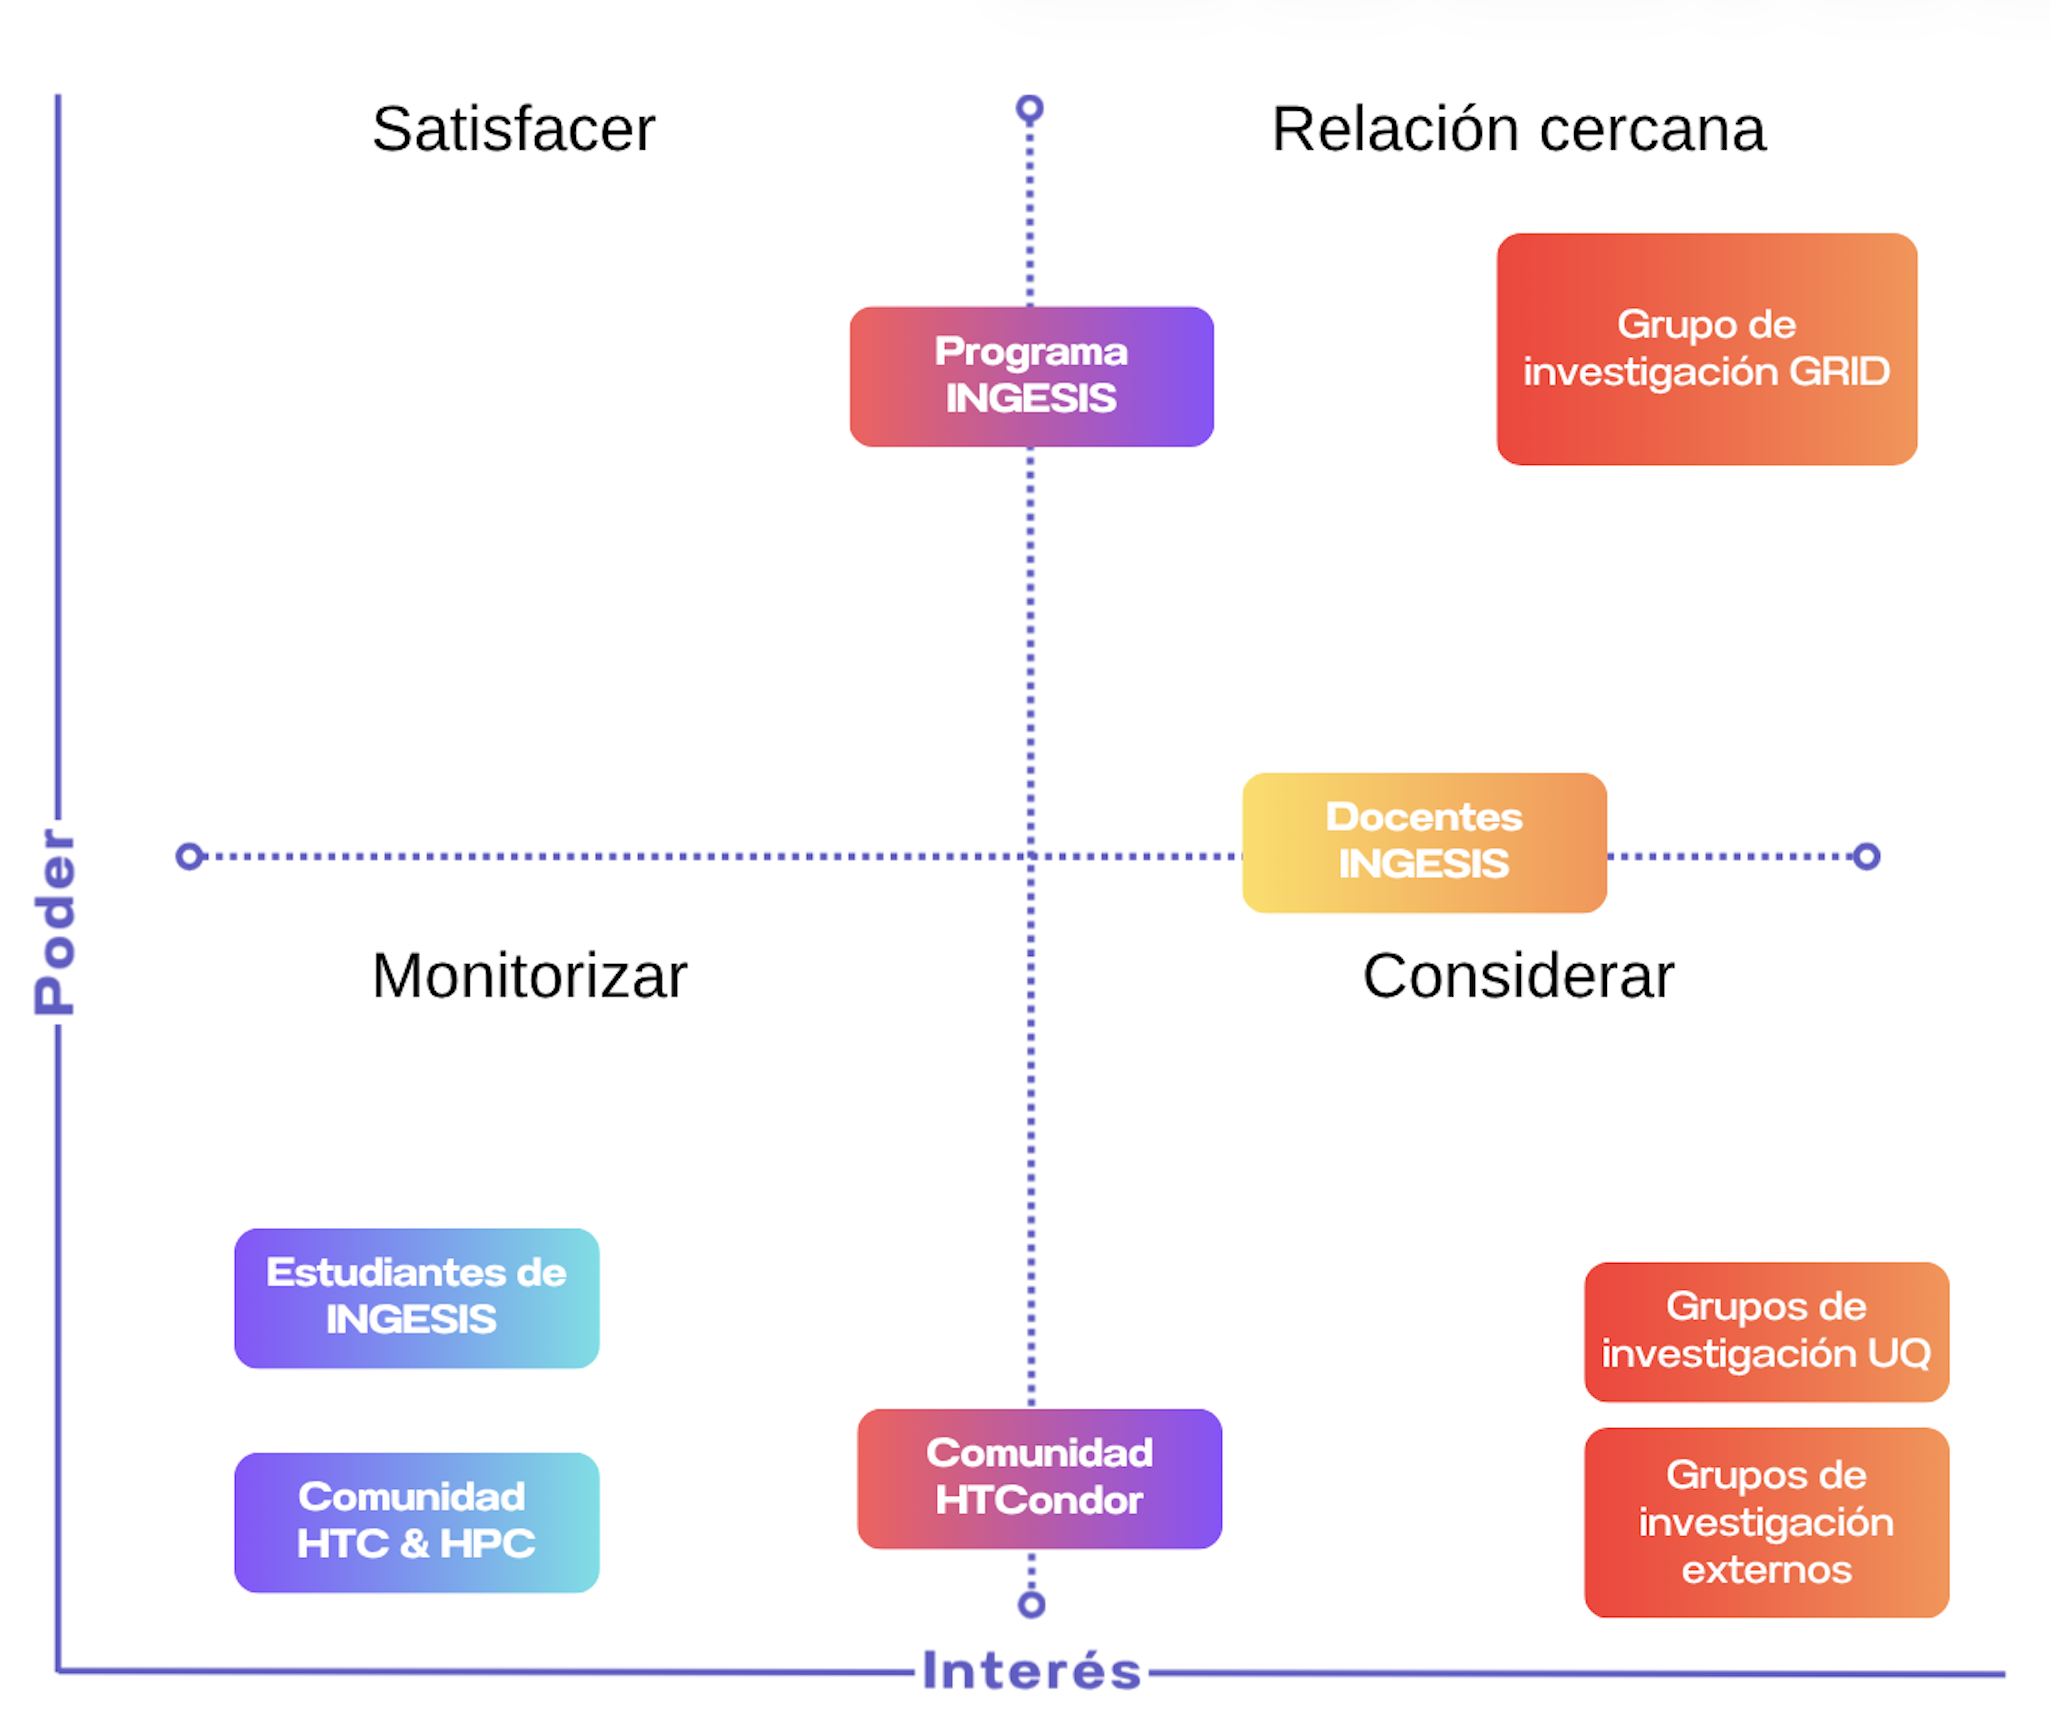
\includegraphics[width=\textwidth] {tablas-images/cp1/priorizacionStakeholders.png}
    \caption{Priorización de stakeholders del proyecto}\label{fig:tabla-priorizacion-stakeholders}
\end{figure}

\section{Integrantes y áreas de trabajo del GRID}
El \GRID\ está conformado por un equipo multidisciplinario de investigadores y profesionales que, desde sus diferentes áreas de experticia, contribuyen al avance en campos como computación de alto rendimiento, \textit{big data}, inteligencia artificial, redes de computadoras y desarrollo de software. A continuación, se presenta una lista de los integrantes actuales del grupo, junto con sus respectivas líneas de trabajo y áreas de especialización:
\begin{itemize}
	\item \href{https://scienti.minciencias.gov.co/cvlac/visualizador/generarCurriculoCv.do?cod_rh=0000210897}{\underline{{\textbf{Christian Andrés Candela Uribe}}}}: Microservicios, desarrollo de software, minería de datos, infraestructura TI.\@
	\item \href{https://scienti.minciencias.gov.co/cvlac/visualizador/generarCurriculoCv.do?cod_rh=0001383939}{\underline{{\textbf{Luis Eduardo Sepúlveda Rodríguez}}}}: Infraestructura de TI, HPC, computación paralela.
	\item \href{https://scienti.minciencias.gov.co/cvlac/visualizador/generarCurriculoCv.do?cod_rh=0001638854}{\underline{{\textbf{Carlos Andrés Flórez Villarraga}}}}: Programación y algoritmia, inteligencia artificial.
	\item \href{https://scienti.minciencias.gov.co/cvlac/visualizador/generarCurriculoCv.do?cod_rh=0001343801}{\underline{{\textbf{Carlos Eduardo Gómez Montoya}}}}: Redes, ingeniería de software, cloud computing.
	\item \href{https://scienti.minciencias.gov.co/cvlac/visualizador/generarCurriculoCv.do?cod_rh=0001398775}{\underline{{\textbf{Sergio Augusto Cardona Torres}}}}: Big data y análisis de datos, ingeniería de software, sistemas adaptativos, informática educativa.
	\item \href{https://scienti.minciencias.gov.co/cvlac/visualizador/generarCurriculoCv.do?cod_rh=0000193550}{\underline{{\textbf{Sonia Jaramillo Valbuena}}}}: Big data, electroquímica, inteligencia artificial.
	\item \href{https://scienti.minciencias.gov.co/cvlac/visualizador/generarCurriculoCv.do?cod_rh=0000283495}{\underline{{\textbf{Julián Esteban Gutiérrez Posada}}}}: Microservicios, desarrollo de software, minería de datos, infraestructura TI, HPC, computación paralela, redes, ingeniería de software.
\end{itemize}

La diversidad de líneas de trabajo de los integrantes fortalece la capacidad del grupo para abordar proyectos de carácter transversal y multidisciplinario, lo cual resulta particularmente relevante para el diseño e implementación de soluciones arquitectónicas soportadas en tecnologías de virtualización.

\section{Misión del GRID}
La misión del GRID es heredada de la Universidad del Quindío. A continuación se presenta la misión del GRID:\@

\begin{quote}
	\textit{La Universidad del Quindío contribuye a la transformación de la sociedad, mediante la formación integral desde el ser, el saber y el hacer, de líderes reflexivos y gestores del cambio; con estándares de calidad, a través de una oferta de formación en diferentes metodologías, que responda a una sociedad basada en el conocimiento; una investigación pertinente, que aporte a la solución de las problemáticas del desarrollo e integrada con la extensión y proyección social; educando en tiempos del posconflicto y de la consolidación de la paz, apoyada en una gestión creativa y con estándares de calidad.}
\end{quote}

A partir de esta misión, se identifican los siguientes pilares fundamentales:

\begin{itemize}
	\item \textbf{Docencia:} La Universidad del Quindío contribuye a la transformación de la sociedad, mediante la formación integral desde el ser, el saber y el hacer, de líderes reflexivos y gestores del cambio; con estándares de calidad, a través de una oferta de formación en diferentes metodologías, que responda a una sociedad basada en el conocimiento.

	\item \textbf{Investigación:} Una investigación pertinente, que aporte a la solución de las problemáticas del desarrollo e integrada con la extensión y proyección social.

	\item \textbf{Extensión y Desarrollo Social:} Apoyada en una gestión creativa y con estándares de calidad.

	\item \textbf{Responsabilidad Social:} Educando en tiempos del posconflicto y de la consolidación de la paz.
\end{itemize}

\section{Visión del GRID}
La misión de la Universidad del Quindío se complementa con su visión institucional, la cual también es adoptada por el \GRID. A continuación se presenta la visión del \GRID:\@

\begin{quote}
	\textit{En el año 2025, la Universidad del Quindío estará consolidada como una institución \textit{Pertinente --- Creativa --- Integradora}, acreditada de alta calidad, con reconocimiento nacional e internacional en sus procesos de formación a través de diferentes metodologías, de investigación, extensión, proyección y responsabilidad social.}
\end{quote}

A partir de esta visión, se destacan los siguientes enfoques estratégicos:

\begin{itemize}
	\item \textbf{Gestión:} La Universidad del Quindío estará consolidada como una institución \textit{Pertinente --- Creativa --- Integradora}.

	\item \textbf{Docencia:} Acreditada de alta calidad en sus procesos de formación a través de diferentes metodologías.

	\item \textbf{Investigación:} Consolidada como pertinente y de alta calidad en sus procesos de investigación.

	\item \textbf{Extensión y Desarrollo Social:} Procesos creativos e integradores en proyección social.

	\item \textbf{Responsabilidad Social:} Reconocimientos en sus procesos de responsabilidad social.
\end{itemize}

\section{Impacto del proyecto en el GRID}
La ampliación de la infraestructura HTCondor mediante la incorporación de un nuevo universo representa un impacto estratégico multidimensional para el Grupo de Investigación GRID. Este proyecto constituye un avance decisivo en la consolidación de una infraestructura de computación distribuida más amplia y capaz, lo que incrementa la competitividad del \GRID en el ámbito de la computación distribuida y de alta productividad. Además, esta expansión podría ayudar a fortalecer el posicionamiento del grupo como referente regional en tecnologías HTC y potenciar su capacidad para establecer colaboraciones interuniversitarias tanto a nivel nacional como internacional.


%%%%% ##############################################################################################################################
%%%%% ##############################################################################################################################
%%%%% ##############################################################################################################################
%%%%% #############################################################################################################################


\section{Caracterización de la infraestructura de computación distribuida del GRID}
\noindent
En la presente sección se especificarán las características técnicas actuales de la infraestructura de computación distribuida HTCondor del grupo \GRID.


% !TODO Verificar el conteo real de la máquinas.
\subsection{Clúster de máquinas Raspberry-Pi}
\noindent

Actualmente, el grupo \GRID cuenta con un clúster compuesto por computadoras Raspberry Pi, distribuidas en nueve torres identificadas como \textbf{Torre 1} a \textbf{Torre 9}. Cada torre contiene siete equipos, con excepción de la Torre 1, que posee únicamente dos: uno opera como nodo maestro y el otro como nodo de envío de tareas. Los equipos restantes de las demás torres funcionan como nodos ejecutores.
\\
Si bien el \GRID posee nueve torres de equipos Raspberry-Pi, la torre novena se encuentra en funcionamiento. \\
%# Tablas de caracterización del GRID 

\begin{table}[h]
	\centering
	\begin{tabular}{|p{6cm}|p{8cm}|}
		\hline
		\multicolumn{2}{|c|}{\textbf{Características las máquinas Raspberry Pi del clúster HTCondor}} \\
		\hline
		Modelo                   & Raspberry Pi 3 Modelo B                                            \\
		\hline
		Versión                  & 1.2                                                                \\
		\hline
		CPU                      & ARMv7 de 1.2GHz                                                    \\
		\hline
		RAM                      & 1 GB                                                               \\
		\hline
		Cantidad de Procesadores & 4                                                                  \\
		\hline
		Sistema Operativo        & Raspbian GNU/Linux 9.1 (stretch) armv7l                            \\
		\hline
		Ubicación                & Oficina tercer piso                                                \\
		\hline
	\end{tabular}
	\caption{Especificaciones de la computadoras Raspberry Pi de GRID}
	\label{table:raspberries-pi-specs}
\end{table}





% Tabla con especificacioens de técnicas de las Raspberry-Pi
En la tabla \ref{table:raspberries-pi-specs} se pueden evidenciar las especificaciones técnicas de las máquinas disponibles para la infraestructura HTCondor del \GRID.
\\


%%#################################  FOTOS TORRES  #########################################
%Image de las Raspberry-Pi
\begin{figure}[H]
	\centering
	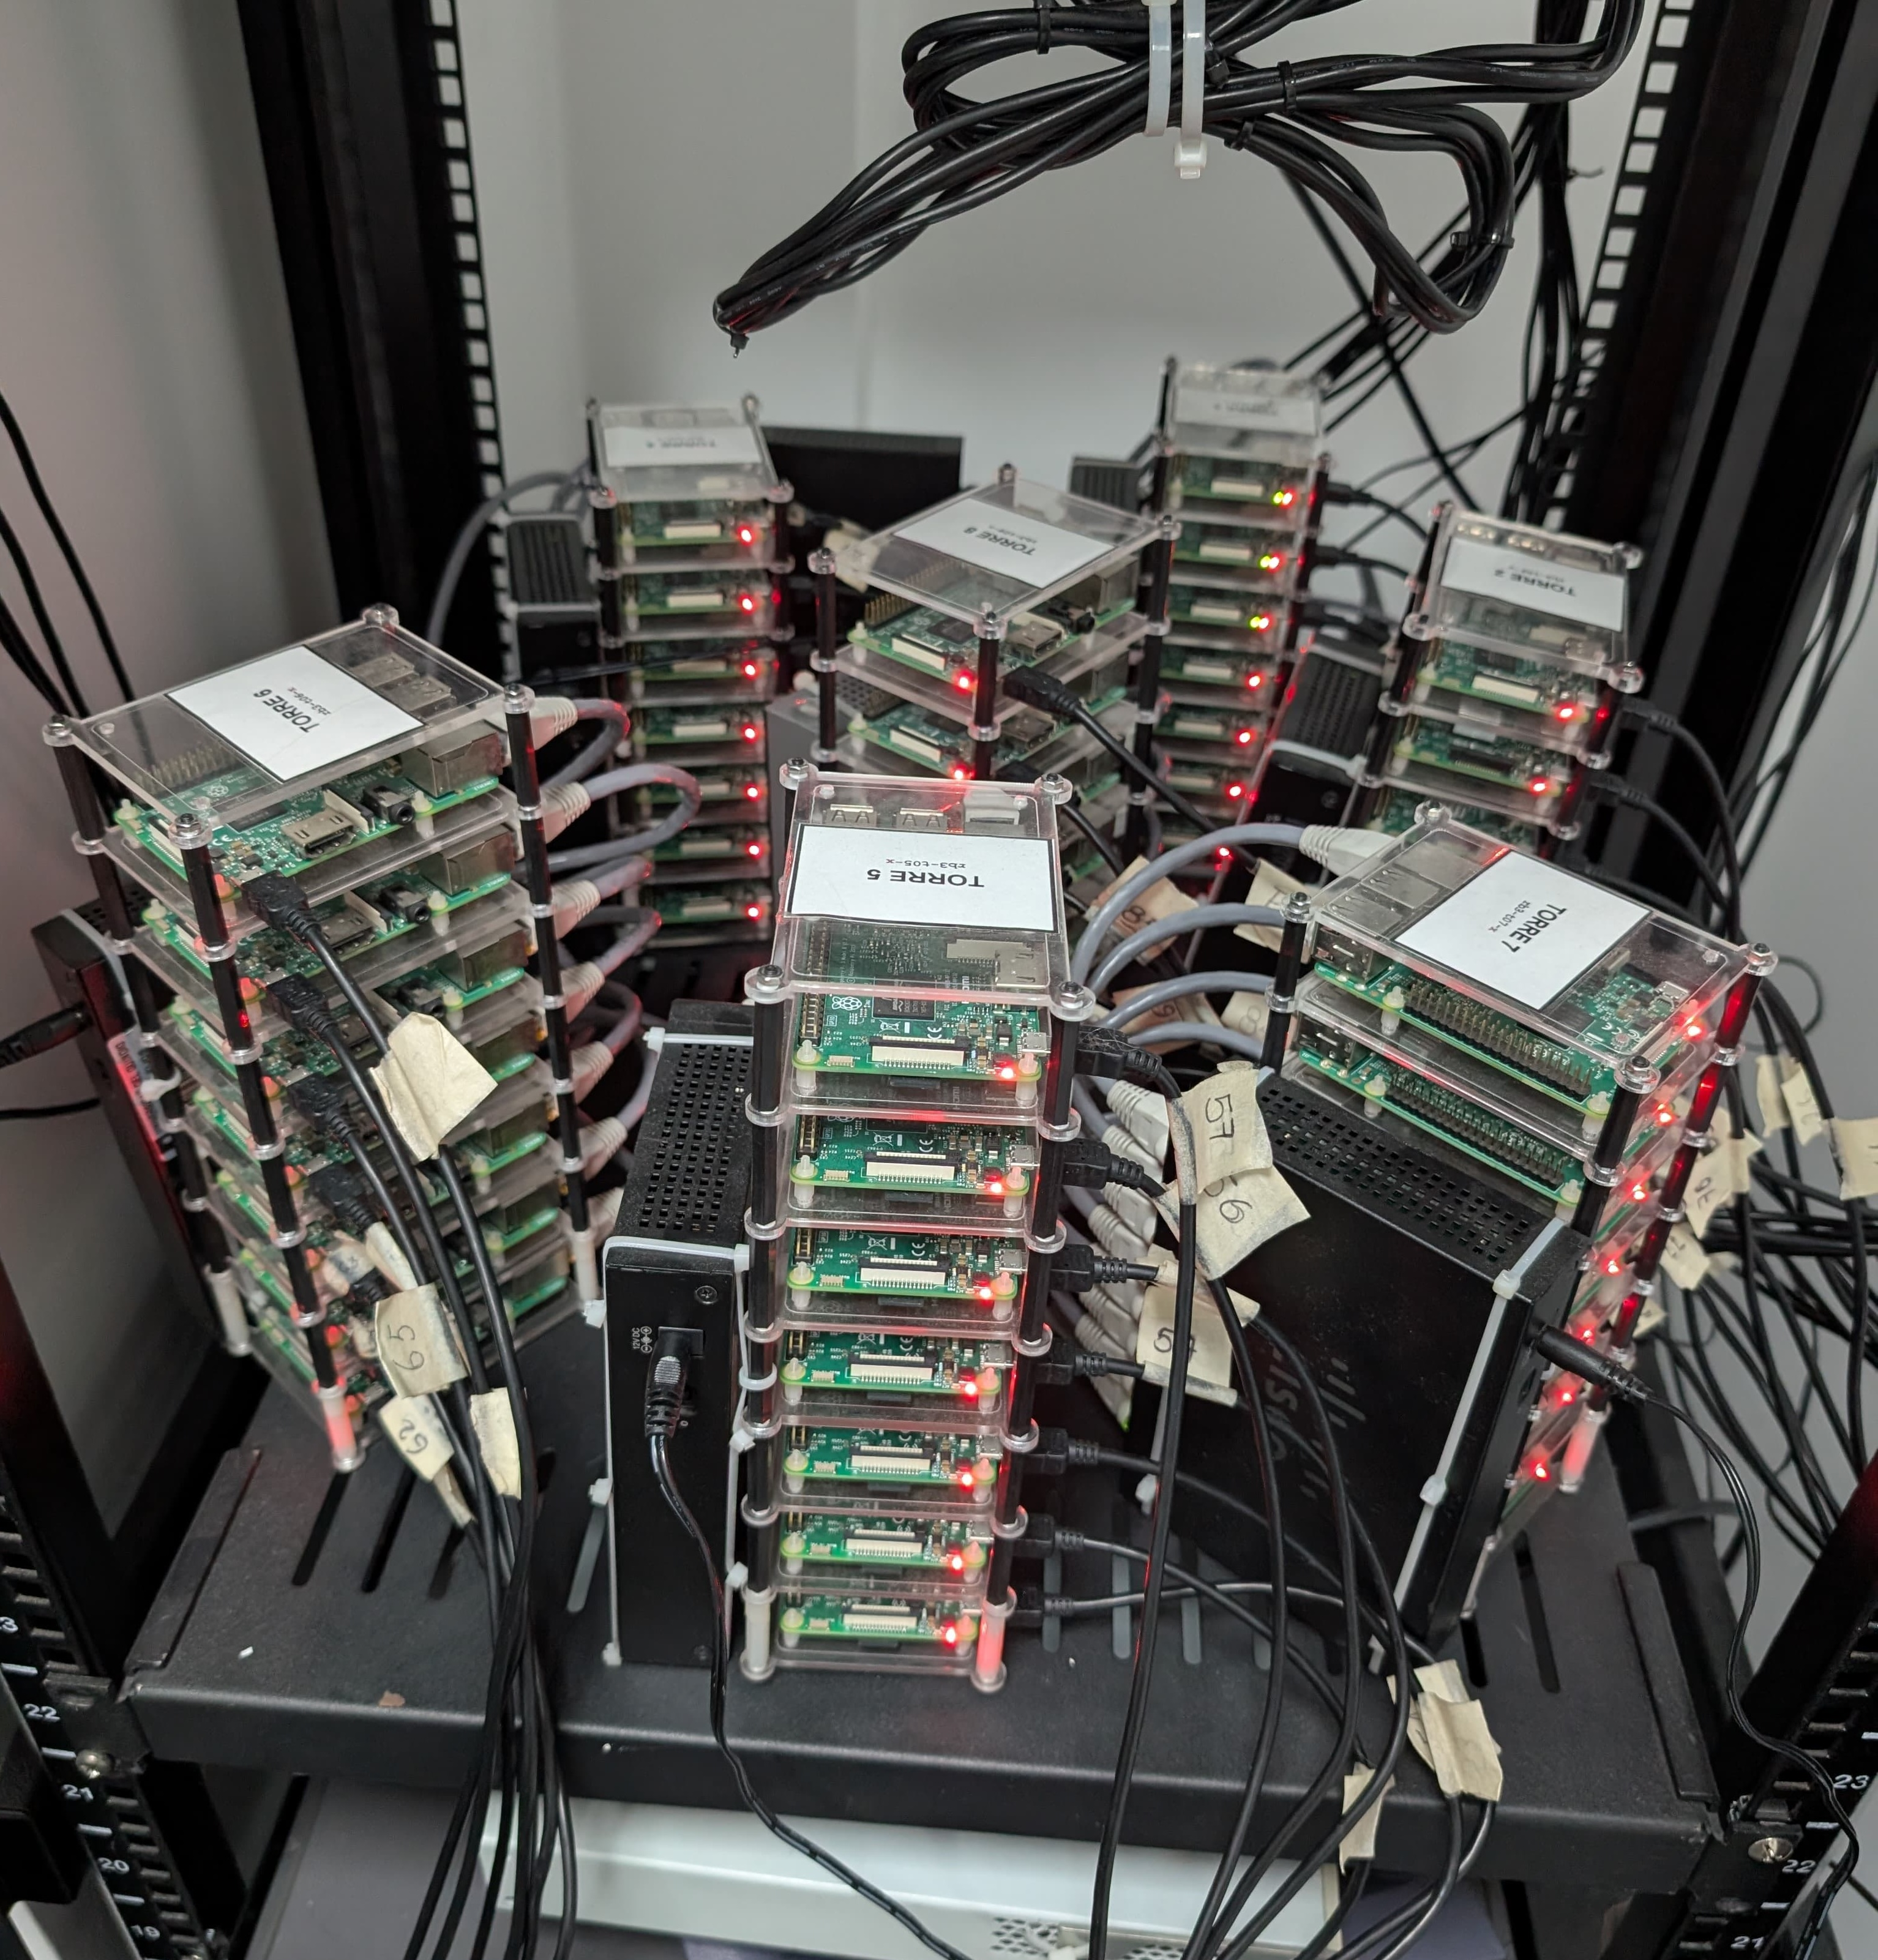
\includegraphics[scale=0.07]{tablas-images/raspberries/torres-raspberries.jpg}
	\caption{Vista general de las maquinas Raspberry-Pi}
	\label{fig:foto-torres-rasp}
\end{figure}


\noindent
En la figura \ref{fig:foto-torres-rasp} se muestra la imagen de las siete torres de Raspberry-Pi localizadas en la oficina del tercer piso de ingeniería. A continuación se muestran las demás torres individualmente.


%Torre BINARIA
\begin{figure}[H]
	\centering
	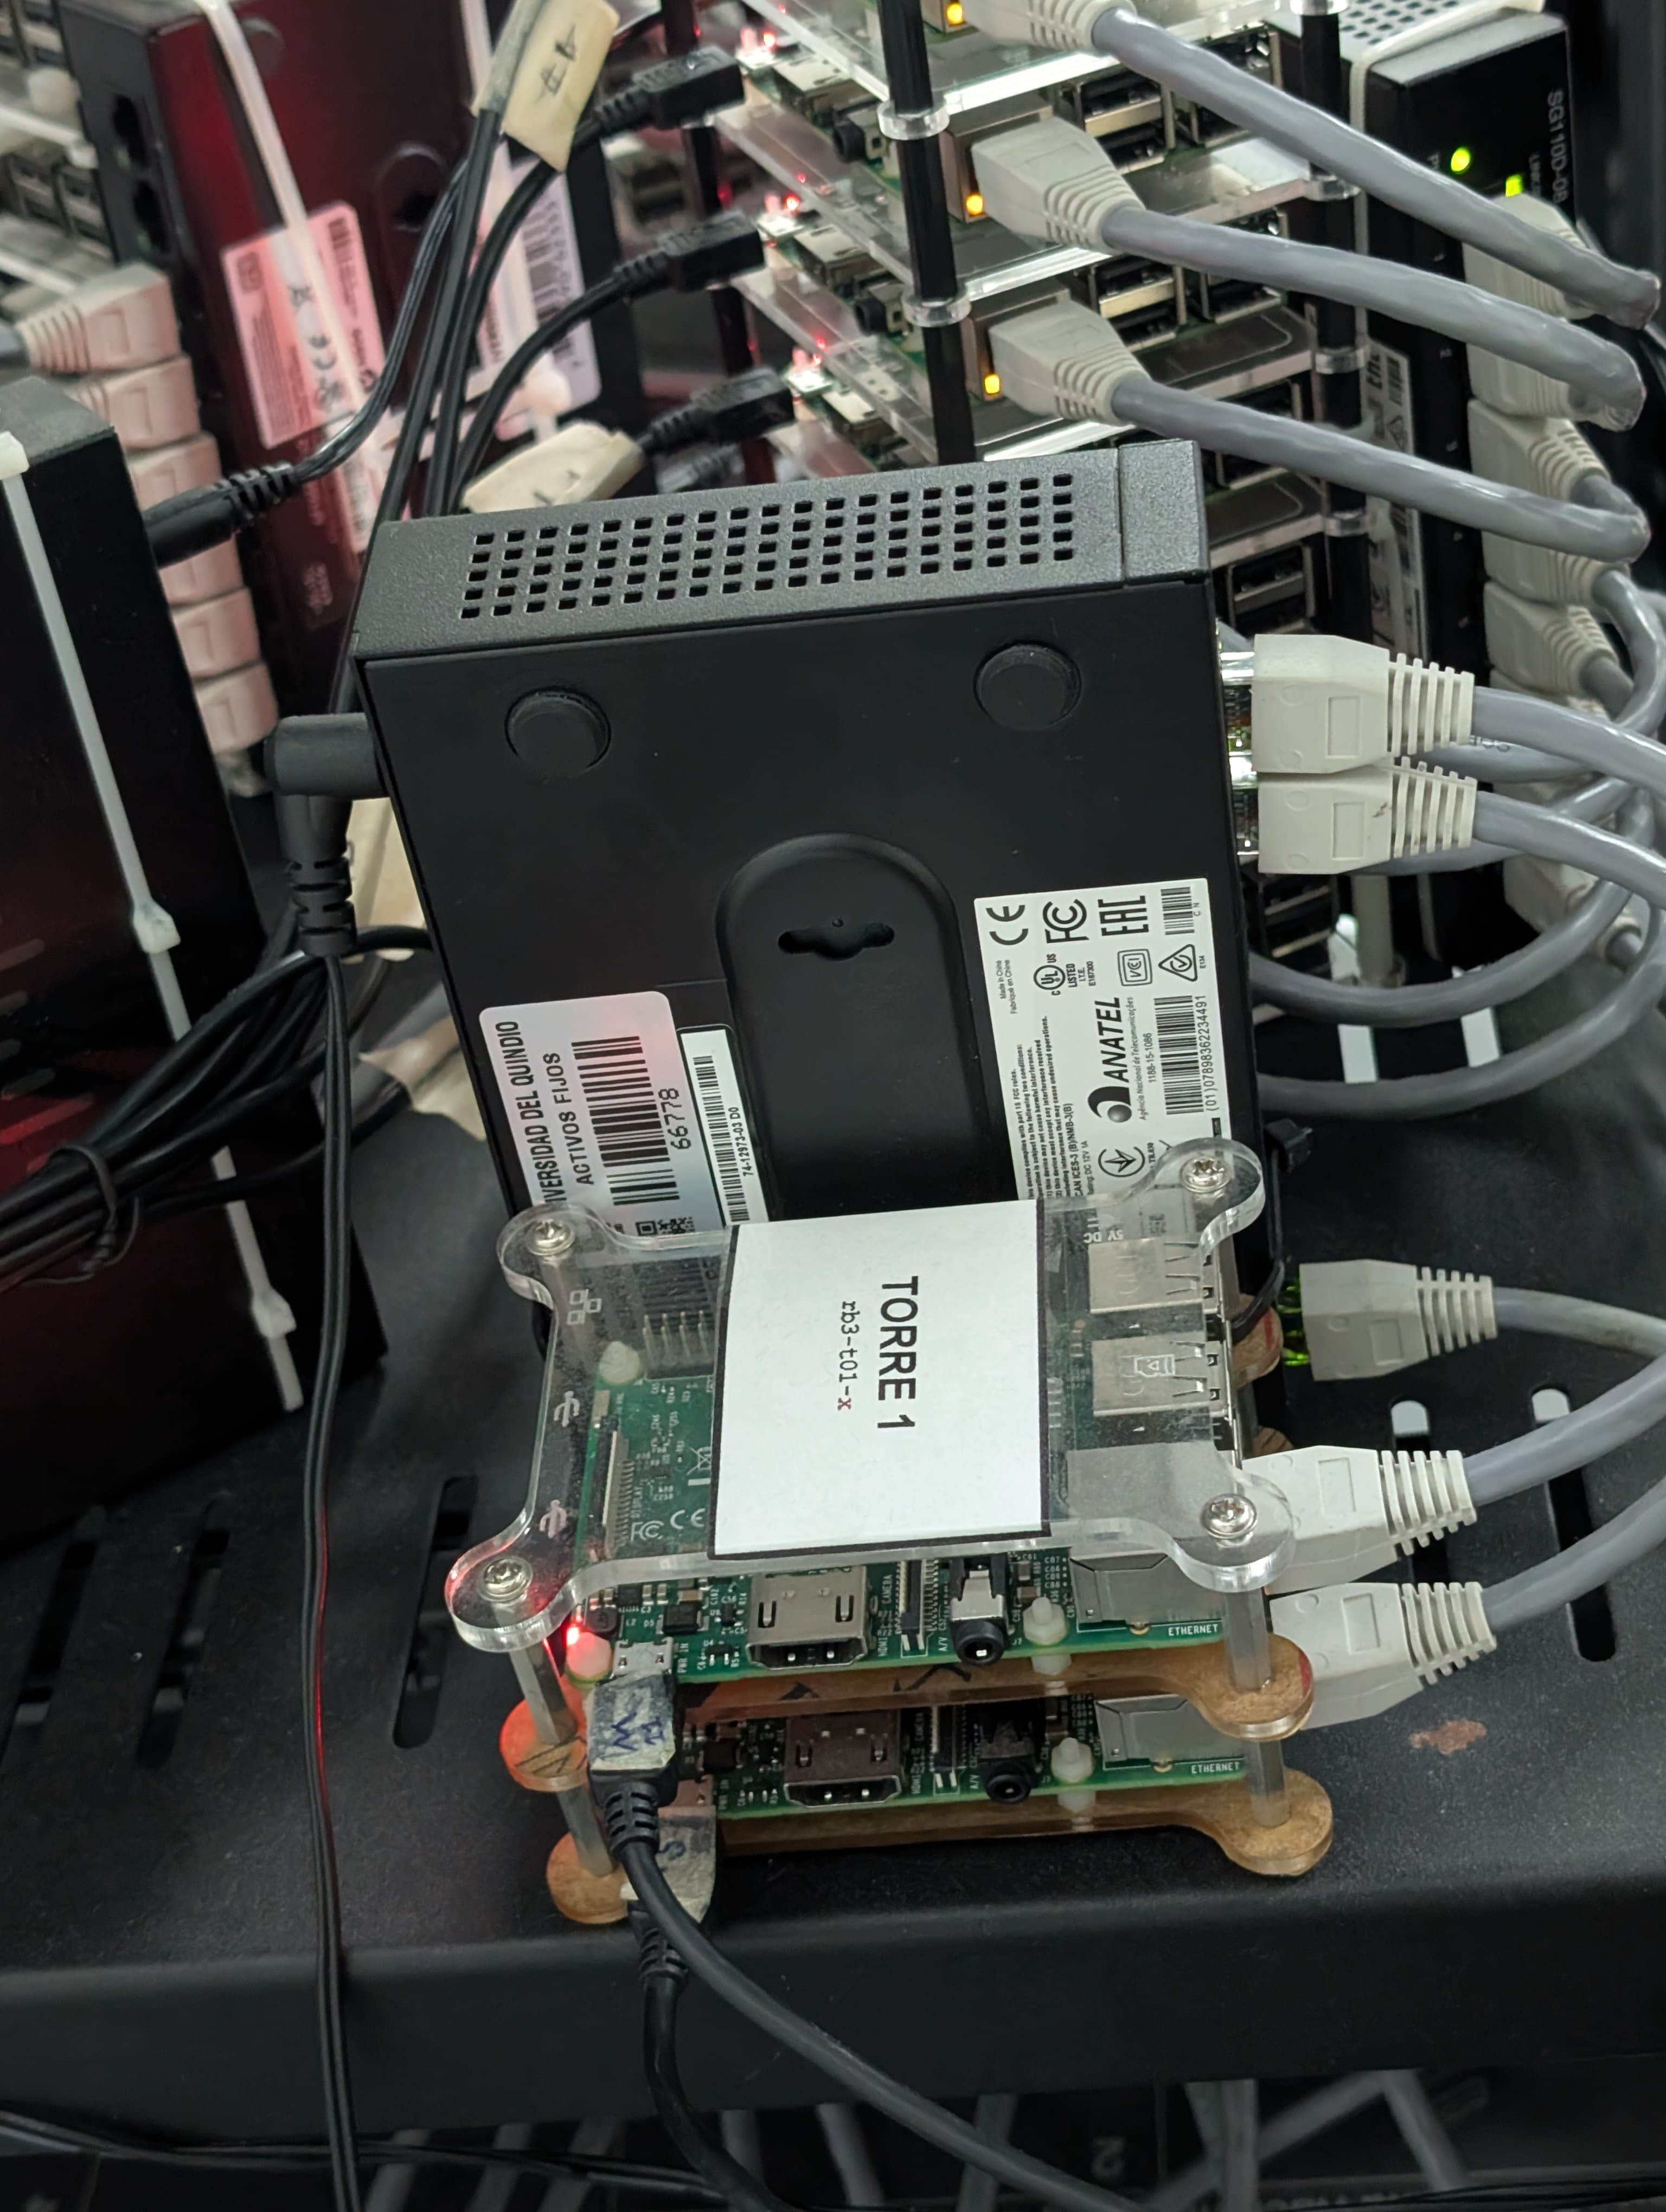
\includegraphics[scale=0.065]{tablas-images/raspberries/torre-binaria.jpeg}
	\caption{Vista general de las máquinas submit y master}
	\label{fig:foto-torre-binaria}
\end{figure}


% ####################################################################################################

\noindent
En la figura \ref{fig:foto-torre-binaria} se muestran las máquinas submit y master de clúster HTCondor.

\noindent
Como se puede evidenciar en las figuras \ref{fig:foto-torres-rasp} y \ref{fig:foto-torre-binaria}, cada máquina perteneciente a una torre está conectada a un switch. Las especificiones de dicho switch se mencionan en la tabla \ref{table:mini-switch}

% filepath: /Users/esteban/git-repos/ht-latex/tablas-images/raspberries/mini-switch.tex
%% Caracteristicas del switch al que están conectadas todas las maquinas HTCondor. 

\begin{table}[H]
	\centering
	\sffamily\scriptsize
	\setlength{\tabcolsep}{4pt}
	\renewcommand{\arraystretch}{1.3}
	\caption{Ficha técnica --- Switch Cisco SF100D-08}\label{table:mini-switch}
	\begin{tabular}{|p{0.25\textwidth}|p{0.6\textwidth}|p{0.12\textwidth}|}
		\hline
		\rowcolor{gray!15} \multicolumn{3}{|c|}{\textbf{DESCRIPCIÓN FÍSICA:} Switch de ocho puertos}                                                                                 \\ \hline

		\textbf{TIPO DE RECURSO:}                    & Switch       & \multirow{3}{*}{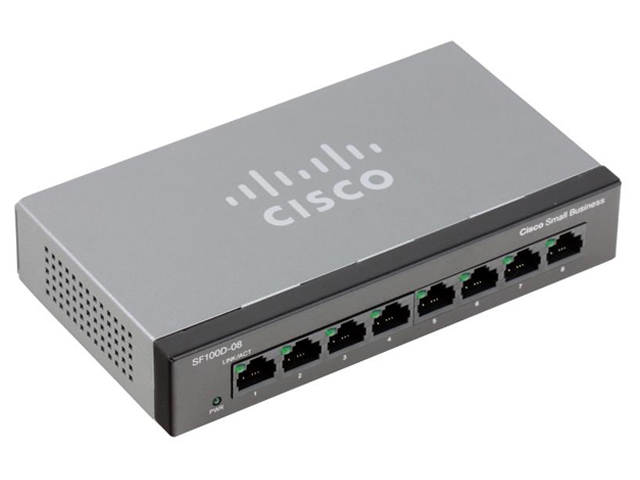
\includegraphics[width=\linewidth,keepaspectratio]{tablas-images/raspberries/mini-switch.jpg}} \\ \cline{1-2}
		\textbf{MODELO:}                             & SF100D-08 V2 &                                                                                                                \\ \cline{1-2}
		\textbf{MARCA:}                              & Cisco        &                                                                                                                \\ \hline

		\rowcolor{gray!15} \multicolumn{3}{|c|}{\textbf{ESPECIFICACIONES TÉCNICAS}}                                                                                                  \\ \hline

		\textbf{Rendimiento}                         &
		\begin{minipage}[t]{\linewidth}
			\vspace{2pt}
			• Capacidad de Conmutación: 1.6 Gbps \\
			• Capacidad de Reenvío: 1.4 mpps \\
			• Prevención de bloqueo HOL \\
			• Jumbo Frames: 9216 bytes
			\vspace{2pt}
		\end{minipage}      &                                                                                                                                         \\ \hline

		\textbf{Interfaces}                          &
		\begin{minipage}[t]{\linewidth}
			\vspace{2pt}
			• 8 puertos RJ-45 10BASE-T/100BASE-TX \\
			• Auto-negociación 10/100 Mbps \\
			• 4 colas de hardware (niveles de prioridad)
			\vspace{2pt}
		\end{minipage} &                                                                                                                                  \\ \hline

		\textbf{Estándares}                          &
		\begin{minipage}[t]{\linewidth}
			\vspace{2pt}
			• 802.3 10BASE-T Ethernet \\
			• 802.3u 100BASE-TX Fast Ethernet \\
			• 802.3x control de flujo \\
			• 802.1p prioridad \\
			• 802.3az Energy Efficient Ethernet
			\vspace{2pt}
		\end{minipage}         &                                                                                                                                           \\ \hline

		\textbf{Características Físicas}             &
		\begin{minipage}[t]{\linewidth}
			\vspace{2pt}
			• Alimentación: DC 12V, 500mA \\
			• Dimensiones: 140 × 33.35 × 140 mm \\
			• Peso: 0.38 kg \\
			• Montaje: Escritorio
			\vspace{2pt}
		\end{minipage}       &                                                                                                                                          \\ \hline

		\textbf{Certificaciones}                     &
		\begin{minipage}[t]{\linewidth}
			\vspace{2pt}
			UL (UL 60950), CSA (CSA 22.2), \\
			CE mark, FCC Part 15 Class A
			\vspace{2pt}
		\end{minipage}            &                                                                                                                                               \\ \hline

		\rowcolor{gray!15} \multicolumn{3}{|l|}{\textbf{PROPÓSITO:} Conexión de red para equipos del cluster HTCondor}                                                               \\ \hline
		\rowcolor{gray!15} \multicolumn{3}{|l|}{\textbf{OPORTUNIDAD DE USO:} Proyectos del \GRID}                                                                                    \\ \hline
		\multicolumn{3}{|p{0.97\textwidth}|}{\textbf{OBSERVACIONES:} Equipo de conectividad que proporciona comunicación entre todos los nodos del cluster HTCondor.}                \\ \hline
	\end{tabular}
\end{table}

\noindent
A su vez, los switch anteriores van conectados a otro switch. Este switch es el Cisco SG200-26. Sus especificaciones pueden verse en la tablas \ref{table:big-switch}

%% Características del switch principal del GRID

\begin{table}[H]
	\centering
	\sffamily\scriptsize
	\setlength{\tabcolsep}{4pt}
	\renewcommand{\arraystretch}{1.3}
	\caption{Ficha técnica --- Switch Cisco SG200-26}
	\label{table:big-switch}
	\begin{tabular}{|p{0.25\textwidth}|p{0.6\textwidth}|p{0.12\textwidth}|}
		\hline
		\rowcolor{gray!15} \multicolumn{3}{|c|}{\textbf{DESCRIPCIÓN FÍSICA:} Switch administrable de 26 puertos}                                                                                                                                 \\ \hline

		\textbf{TIPO DE RECURSO:}                     & Switch Gigabit administrable & \multirow{3}{*}{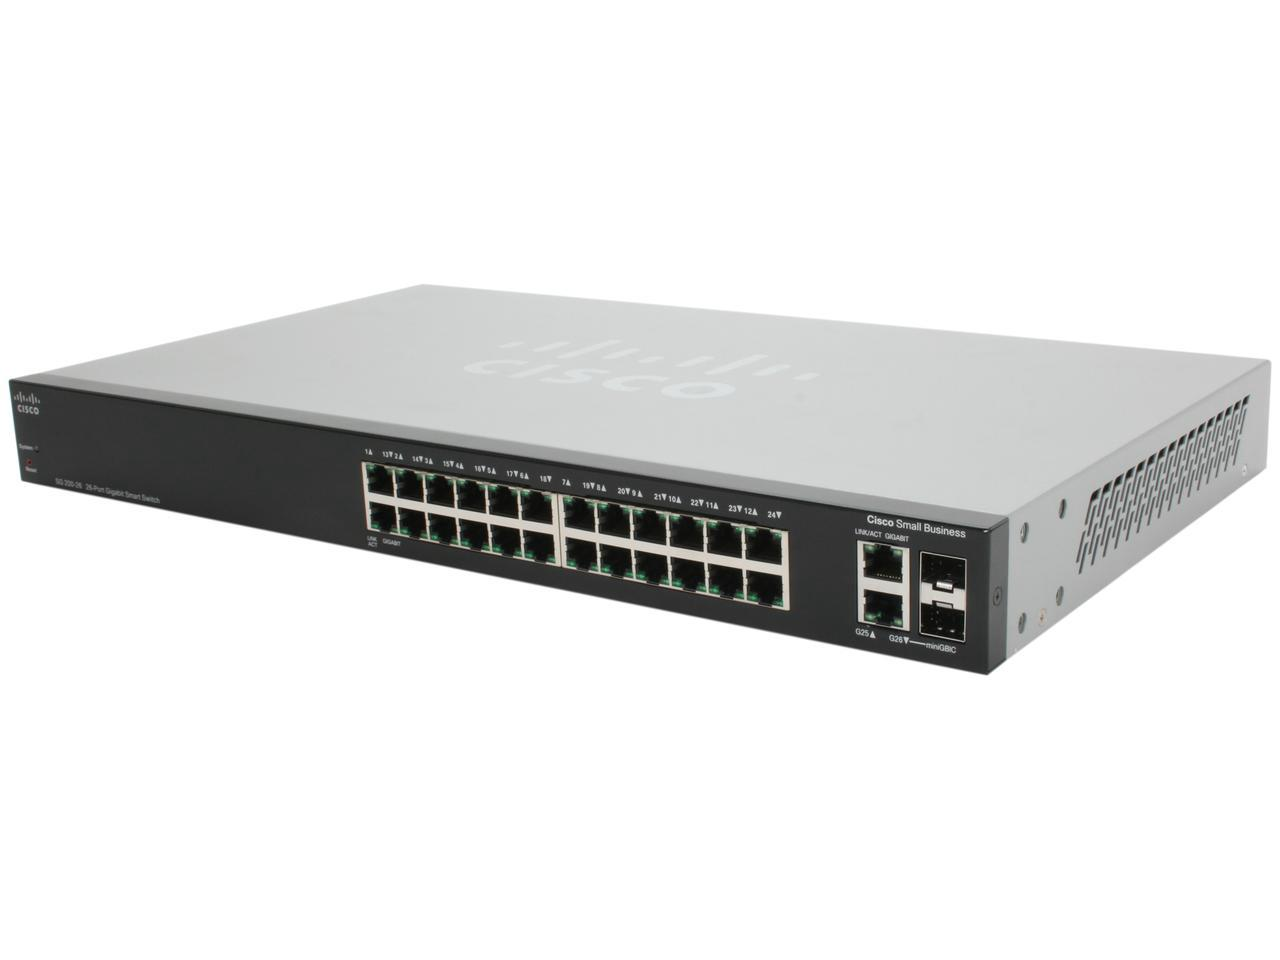
\includegraphics[width=\linewidth,keepaspectratio]{tablas-images/raspberries/big-switch.jpg}}                                             \\ \cline{1-2}
		\textbf{MODELO:}                              & SG200-26                     &                                                                                                                                                           \\ \cline{1-2}
		\textbf{MARCA:}                               & Cisco                        &                                                                                                                                                           \\ \hline

		\rowcolor{gray!15} \multicolumn{3}{|c|}{\textbf{ESPECIFICACIONES TÉCNICAS}}                                                                                                                                                              \\ \hline

		\textbf{Rendimiento}                          &
		\begin{minipage}[t]{\linewidth}
			\vspace{2pt}
			• Capacidad de Conmutación: 52 Gbps \\
			• Capacidad de Reenvío: 38.69 Mpps \\
			• Tabla de direcciones MAC: 8,000 entradas \\
			• Jumbo Frames: Soportado
			\vspace{2pt}
		\end{minipage} &                                                                                                                                                                                               \\ \hline

		\textbf{Interfaces}                           &
		\begin{minipage}[t]{\linewidth}
			\vspace{2pt}
			• 24 puertos RJ-45 10/100/1000 Mbps \\
			• 2 puertos combo Gigabit SFP \\
			• Auto-negociación y auto-MDI/MDIX \\
			• Soporte IEEE 802.3ad (Link Aggregation)
			\vspace{2pt}
		\end{minipage}     &                                                                                                                                                                                                 \\ \hline

		\textbf{Administración}                       &
		\begin{minipage}[t]{\linewidth}
			\vspace{2pt}
			• Interfaz web de administración \\
			• SNMP, RMON, HTTP, TFTP \\
			• Cisco Discovery Protocol \\
			• Auto SmartPorts \\
			• Soporte DHCP y BOOTP
			\vspace{2pt}
		\end{minipage}           &                                                                                                                                                                                                         \\ \hline

		\textbf{Características Avanzadas}            &
		\begin{minipage}[t]{\linewidth}
			\vspace{2pt}
			• VLAN support (IEEE 802.1Q) \\
			• Quality of Service (QoS) \\
			• IGMP/MLD Snooping \\
			• Spanning Tree (STP/RSTP) \\
			• IEEE 802.1x Authentication \\
			• Storm Control (Broadcast/Multicast/Unicast)
			\vspace{2pt}
		\end{minipage} &                                                                                                                                                                                             \\ \hline

		\textbf{Características Físicas}              &
		\begin{minipage}[t]{\linewidth}
			\vspace{2pt}
			• Alimentación: 100-240V AC, 50-60 Hz \\
			• Dimensiones: 439 × 257 × 43 mm \\
			• Peso: 3.3 kg (7.2 lbs) \\
			• Montaje: Rack 1U \\
			• Diseño sin ventiladores
			\vspace{2pt}
		\end{minipage}      &                                                                                                                                                                                                    \\ \hline

		\textbf{Memoria y Estándares}                 &
		\begin{minipage}[t]{\linewidth}
			\vspace{2pt}
			• Flash: 16 MB, RAM: 128 MB \\
			• IEEE 802.3/802.3u/802.3z/802.3ab \\
			• Certificaciones: UL 60950, FCC Part 15A \\
			• MTBF: 194,278 horas
			\vspace{2pt}
		\end{minipage}  &                                                                                                                                                                                                \\ \hline

		\rowcolor{gray!15} \multicolumn{3}{|l|}{\textbf{PROPÓSITO:} Switch principal para interconexión de infraestructura GRID}                                                                                                                 \\ \hline
		\rowcolor{gray!15} \multicolumn{3}{|l|}{\textbf{OPORTUNIDAD DE USO:} Backbone de red para servicios del \GRID}                                                                                                                           \\ \hline
		\multicolumn{3}{|p{0.97\textwidth}|}{\textbf{OBSERVACIONES:} Switch administrable de nivel empresarial que proporciona conectividad Gigabit con funciones avanzadas de gestión, VLAN, QoS y seguridad para la infraestructura del GRID.} \\ \hline
	\end{tabular}
\end{table}


\subsection{Ambientes de ejecución de la infraestructura HTCondor del \GRID}
\noindent{}
De acuerdo con la documentación oficial de HTCondor \citep{HTCondor-choosing-universe}, un universo se define como el ambiente de ejecución en el cual se lleva a cabo un trabajo. Al momento del desarrollo de la presente investigación, HTCondor contempla nueve universos disponibles: \textit{vanilla, grid, java, scheduler, local, parallel, vm, container} y \textit{docker}. Cada trabajo demanda, en función de sus características particulares, condiciones específicas de ejecución. A modo de ejemplo, un trabajo constituido por un programa desarrollado en lenguaje Java puede obtener ventajas significativas mediante la utilización del universo Java, lo cual facilita al usuario la configuración del ambiente de ejecución requerido.

Hasta el momento, la configuración de HTCondor del \GRID únicamente incorpora el universo vanilla, el cual está orientado a la ejecución no especializada de programas. En otras palabras, se trata de un universo de propósito general en el que los scripts de Shell han demostrado ser particularmente efectivos \citep{HTCondor-choosing-universe}.


\subsection{Servicios actuales de computación distribuida}
\noindent
Los servicios actuales del \GRID se orientan principalmente hacia la provisión de infraestructura de \TI, abarcando máquinas virtuales, soluciones de almacenamiento y configuración de redes. No obstante, la computación distribuida constituye un dominio especializado que demanda competencias técnicas avanzadas por parte de los usuarios. En consecuencia, si bien el grupo ha desarrollado capacidades en esta área, aún no se ha consolidado una oferta formal de servicios de computación distribuida de acceso público para la comunidad académica institucional.

% !TODO PREGUNTA PARA EL PROFE: Aquí hago una declaración temeraria sobre la universidad que neceisto confirmar
% Se han ofrecido servicios de computación identifica en el grupo grid que hayan estado disponibles para otros grupos o para 
% los mismo estudiantes de la universidad? 
%
\subsection{Servicios de computación distribuida esperados}
\noindent
Dado que no se ha establecido previamente un servicio de computación distribuida basado en HTCondor con acceso abierto para la comunidad educativa, resulta necesario identificar los potenciales beneficiarios que podrían aprovechar de manera más efectiva esta tecnología. Como señalan \cite{Wilson2016}, la computación se ha consolidado como un componente crítico del proceso científico en prácticamente todas las disciplinas, independientemente de su orientación hacia la experimentación o la simulación computacional. En este contexto, los usuarios que obtendrían mayor beneficio de la implementación de un servicio de computación distribuida serían aquellos cuyas actividades académicas o investigativas demanden capacidades de procesamiento intensivo para la obtención de resultados científicos. Por consiguiente, se estima que los principales beneficiarios de esta infraestructura serían tanto los estudiantes, quienes podrían fortalecer significativamente su proceso formativo mediante el acceso a una ambiente de computación distribuida, como los grupos de investigación institucionales, que verían ampliadas sus capacidades para desarrollar proyectos de mayor envergadura computacional. En la tabla \ref{table:servicio-htcondor} se especifica cómo podría verse un servicio de computación de alta productividad en  basado en HTcondor.

\begin{table}[H]
	\centering
	\sffamily\scriptsize
	\setlength{\tabcolsep}{4pt}
	\renewcommand{\arraystretch}{1.3}
	\caption{Caracterización del servicio de computación distribuida HTCondor esperado para el GRID}
	\label{table:servicio-htcondor}
	\begin{tabular}{|p{0.28\textwidth}|p{0.67\textwidth}|}
		\hline
		\rowcolor{gray!15} \multicolumn{2}{|c|}{\textbf{DESCRIPCIÓN GENERAL DEL SERVICIO}}                                                                                                                                                                                            \\ \hline

		\textbf{NOMBRE DEL SERVICIO}       & Servicio de Computación Distribuida HTCondor                                                                                                                                                                                             \\ \hline
		\textbf{TIPO DE SERVICIO}          & Servicio de educación, investigación y extensión universitaria                                                                                                                                                                           \\ \hline
		\textbf{HORARIO DE DISPONIBILIDAD} & 24/7 (Disponibilidad continua)                                                                                                                                                                                                           \\ \hline

		\rowcolor{gray!15} \multicolumn{2}{|c|}{\textbf{OBJETIVOS Y ALCANCE}}                                                                                                                                                                                                         \\ \hline

		\textbf{PROPÓSITO}                 &
		\begin{minipage}[t]{\linewidth}
			\vspace{2pt}
			Proveer infraestructura de computación de alta productividad (\HTC) para la ejecución de tareas computacionales intensivas y paralelas, facilitando el procesamiento distribuido de cargas de trabajo científicas y académicas
			\vspace{2pt}
		\end{minipage}                                                 \\ \hline

		\textbf{USUARIOS OBJETIVO}         &
		\begin{minipage}[t]{\linewidth}
			\vspace{2pt}
			• Estudiantes de pregrado y posgrado \\
			• Grupos de investigación institucionales \\
			• Docentes investigadores \\
			• Comunidad académica UQ
			\vspace{2pt}
		\end{minipage}                                                                                                                                                                                                                                     \\ \hline

		\rowcolor{gray!15} \multicolumn{2}{|c|}{\textbf{ESPECIFICACIONES TÉCNICAS}}                                                                                                                                                                                                   \\ \hline

		\textbf{RECURSOS DE HARDWARE}      &
		\begin{minipage}[t]{\linewidth}
			\vspace{2pt}
			• Clúster de máquinas Raspberry Pi \\
			• Máquinas virtuales especializadas \\
			• Infraestructura de red dedicada
			\vspace{2pt}
		\end{minipage}                                                                                                                                                                                                                                           \\ \hline

		\textbf{TECNOLOGÍAS}               &
		\begin{minipage}[t]{\linewidth}
			\vspace{2pt}
			• HTCondor (High Throughput Computing) \\
			• Sistemas de virtualización \\
			• Administración de cola de trabajos
			\vspace{2pt}
		\end{minipage}                                                                                                                                                                                                                                        \\ \hline

		\textbf{CAPACIDADES}               &
		\begin{minipage}[t]{\linewidth}
			\vspace{2pt}
			• Procesamiento paralelo de tareas independientes \\
			• Gestión automática de recursos \\
			• Balanceamiento de carga dinámico \\
			• Tolerancia a fallos
			\vspace{2pt}
		\end{minipage}                                                                                                                                                                                                                             \\ \hline

		\rowcolor{gray!15} \multicolumn{2}{|c|}{\textbf{APLICACIONES Y BENEFICIOS}}                                                                                                                                                                                                   \\ \hline

		\textbf{CASOS DE USO}              &
		\begin{minipage}[t]{\linewidth}
			\vspace{2pt}
			• Simulaciones científicas y modelado matemático \\
			• Procesamiento de datos masivos (Big Data) \\
			• Renderización de video y gráficos \\
			• Análisis bioinformático y genómico \\
			\vspace{2pt}
		\end{minipage}                                                                                                                                                                                                                              \\ \hline

		\textbf{IMPACTO ESPERADO}          &
		\begin{minipage}[t]{\linewidth}
			\vspace{2pt}
			• Fortalecimiento de capacidades investigativas \\
			• Democratización del acceso a recursos HTC \\
			• Apoyo a formación en computación distribuida \\
			• Incremento en productividad científica \\
			• Posicionamiento institucional en \HTC
			\vspace{2pt}
		\end{minipage}                                                                                                                                                                                                                               \\ \hline

		\rowcolor{gray!15} \multicolumn{2}{|l|}{\textbf{CONTRIBUCIÓN:} Expansión de universos HTCondor para mayor versatilidad}                                                                                                                                                       \\ \hline
		\multicolumn{2}{|p{0.95\textwidth}|}{\textbf{OBSERVACIONES:} Servicio orientado a democratizar el acceso a recursos de computación de alto rendimiento para la comunidad académica, fortaleciendo las capacidades investigativas y formativas de la Universidad del Quindío.} \\ \hline
	\end{tabular}
\end{table}
\section{Descripción de la oportunidad}
\noindent
La implementación de un nuevo universo HTCondor en la infraestructura del grupo GRID representa una oportunidad estratégica de considerable valor tanto para la comunidad académica de la Universidad del Quindío como para los grupos de investigación locales y externos. En primer lugar, esta ampliación abrirá el paso para que diversos grupos de investigación de la institución accedan a capacidades computacionales especializadas más diversas, democratizando así el uso de tecnologías de computación distribuida para disciplinas que requieren procesamiento intensivo de datos, tales como la bioinformática, el análisis de big data, el aprendizaje profundo y la simulación científica. En segundo lugar, desde una perspectiva formativa, la incorporación de este nuevo universo constituye una oportunidad invaluable para que los estudiantes de pregrado y posgrado adquieran competencias prácticas en computación de alto rendimiento (\HTC), un campo con limitada documentación y experiencias de implementación documentadas en el contexto colombiano. Adicionalmente, esta iniciativa ayudaría al posicionamiento del \GRID como un referente en computación distribuida a nivel nacional, facilitando la colaboración interinstitucional y el desarrollo de proyectos conjuntos con otras universidades e instituciones de investigación. Finalmente, la consolidación de una infraestructura HTCondor más robusta y versátil contribuye directamente a la competitividad investigativa de la Universidad del Quindío, optimizando el aprovechamiento de recursos computacionales disponibles y generando capacidades técnicas diferenciadas que pueden traducirse en publicaciones científicas, proyectos de mayor envergadura y fortalecimiento de las líneas de investigación institucionales.


\section{Resumen de la entrevista con el cliente}

Para comprender mejor las necesidades y expectativas del \GRID\, se realizó una entrevista con el cliente.

%!TODO  Entrevista
\begin{itemize}
	\item \textbf{Entrevistado:} Luis Eduardo Sepúlveda Rodríguez
	\item \textbf{Fecha:} XXXXXXXXX
	\item \textbf{Duración:} XXXXXXXXXXX
	\item \textbf{Link:} \href{https://drive.google.com}{click aquí}
	\item \textbf{Asistentes:} Juan Esteban Castaño Osma, Juan Esteban Parra Parra
\end{itemize}

%\ChapterImageStar[cap:revisionLiteratura]{Revisión sistemática de la literatura}{./images/fondo.png}\label{cap:revisionLiteratura}

\mbox{}\\
\section{Construcción de la bitácora}

En busca de una base teórica sólida para seleccionar un nuevo universo HTCondor y con el objetivo de tomar decisiones informadas, se llevó a cabo una revisión exhaustiva de la literatura existente sobre el tema. Este proceso se desarrolló en varias etapas:


\subsection{Planeación}

Esta etapa consistió en establecer el propósito general que se buscaba alcanzar con el \SMS (\textit{Systematic Mapping Study}).
A su vez, definió aspectos como objetivos ver cuadro ~\ref{tab:metas}, preguntas de investigación ver cuadro~\ref{tab:preguntas} y métricas ver cuadro~\ref{tab:metricas}. Para ello, se siguió el modelo
Objetivo-Pregunta-Métrica (\textit{goal-question-metric}, gqm). A continuación, se definen los objetivos del \SMS\ aplicado
a los universos de HTCondor en el cuadro.

\subsubsection{Definición de metas para el \SMS}

\begin{table}[H]
	\centering
	\renewcommand{\arraystretch}{1.2} % Espaciado reducido
	\footnotesize % Texto más pequeño
	\begin{tabular}{|>{\centering\arraybackslash}p{1.5cm}|p{12.5cm}|}  % Total: 14cm
		\hline
		\textbf{Meta} & \textbf{Descripción}                                                                                                                                                                                                                                                                                                                                         \\ \hline
		G1            & Clasificar trabajos relacionados con los universos de HTCondor según su aplicación e impacto en los dominios de computación distribuida y paralela, HTC, desarrollo de Software, virtualización y microservicios, redes de computadoras, infraestructura computacional, inteligencia artificial, análisis de datos y pensamiento computacional, entre otros. \\ \hline
		G2            & Identificar y categorizar trabajos vinculados con los universos de HTCondor como herramienta para fortalecer funciones esenciales universitarias como: investigación, docencia, extensión e industria.                                                                                                                                                       \\ \hline
	\end{tabular}
	\caption{Definición de metas del SMS}
	\label{tab:metas}
\end{table}

\subsubsection{Definición de preguntas de investigación}
\begin{table}[H]
	\centering
	\renewcommand{\arraystretch}{1.2} % Espaciado reducido
	\scriptsize % Texto más pequeño
	\begin{tabular}{|>{\centering\arraybackslash}p{0.7cm}|>{\centering\arraybackslash}p{1.3cm}|p{5.5cm}|p{6cm}|} % Total: 14cm
		\hline
		\textbf{Meta}                                                                                                                                                                                                                                                                                                                                    & \textbf{Pregunta} & \textbf{Descripción} & \textbf{Motivación}       \\ \hline

		G1                                                                                                                                                                                                                                                                                                                                               & Q1                &
		\textit{¿Qué trabajos relacionados con los universos de HTCondor tienen impacto en los dominios de computación distribuida y paralela, HTC, desarrollo de Software, virtualización y microservicios, redes de computadoras, infraestructura computacional, inteligencia artificial, análisis de datos y pensamiento computacional, entre otros?} &
		Sobre los universos de HTCondor que tienen impacto en los dominios de computación distribuida y paralela, HTC, desarrollo de Software, virtualización y microservicios, redes de computadoras, infraestructura computacional, inteligencia artificial, análisis de datos, pensamiento computacional: 1 - Reconocer cómo están estructurados. 2 - Identificar sus aplicaciones. 3 - Determinar su motivación contextual. \\ \hline

		G2                                                                                                                                                                                                                                                                                                                                               & Q2                &
		\textit{¿Qué trabajos vinculados con los universos de HTCondor potencian las funciones esenciales universitarias como investigación, docencia, extensión e industria?}                                                                                                                                                                           &
		Sobre los universos de HTCondor que potencian las funciones sustantivas universitarias como investigación, docencia, extensión e industria: 1 - Reconocer cómo están estructurados. 2 - Identificar sus aplicaciones. 3 - Determinar su motivación contextual.                                                                                                                                                          \\ \hline
	\end{tabular}
	\caption{Definición de preguntas de investigación del SMS}
	\label{tab:preguntas}
\end{table}

\subsubsection{Definición de métricas}

\begin{table}[H]
	\centering
	\renewcommand{\arraystretch}{1.2} % Menor espaciado entre filas
	\footnotesize % Texto más pequeño
	\begin{tabular}{|c|p{13cm}|} % Total: 14cm
		\hline
		\textbf{Métrica} & \textbf{Descripción}                                                                                                                                                                                                                                                                                                                                                                                                                                                                                           \\ \hline
		M1               & Cantidad de trabajos relacionados con los Universos de HTCondor vinculados con los dominios de: Computación distribuida y paralela, HTC, Desarrollo de software, Tecnologías de virtualización y microservicios, Redes de computadores, Infraestructura computacional, Inteligencia artificial, Análisis de datos, Pensamiento computacional, entre otros. Y que además sean usados como herramienta para fortalecer funciones esenciales universitarias como: Investigación, Docencia, Extensión e Industria. \\ \hline
		M2               & Popularidad de cada Universo en los trabajos seleccionados.                                                                                                                                                                                                                                                                                                                                                                                                                                                    \\ \hline
		M3               & Porcentaje de trabajos seleccionados en la fase final respecto de la cantidad de trabajos iniciales.                                                                                                                                                                                                                                                                                                                                                                                                           \\ \hline
		M4               & Porcentaje de trabajos aportados por cada base de datos en el mapeo que se está desarrollando.                                                                                                                                                                                                                                                                                                                                                                                                                 \\ \hline
	\end{tabular}
	\caption{Definición de métricas del SMS}
	\label{tab:metricas}
\end{table}

\section{Búsqueda de estudios}

Esta etapa comprendió las siguientes secciones:
\begin{enumerate}
	\item Estrategia de búsqueda, ya sea independiente o combinada;
	\item Identificación general de estudios;
	\item Revisión de estudios; y finalmente,
	\item Selección de estudios para incluir en el SMS.\@
\end{enumerate}

\subsection{Estrategia de búsqueda}

Este trabajo combinó las estrategias de búsqueda en bases de datos y búsqueda en bola de nieve.
Para la estrategia de búsqueda en bases de datos, se seleccionaron las siguientes bases de datos: ACM, IEEE Xplore, Springer, Taylor \& Francis y Science Direct.

\subsection{Búsqueda en bases de datos}\label{subsec:busquedaBasesDatos}
Se seleccionaron las siguientes bases de datos para este propósito: ACM, IEEE Xplore, Springer, Taylor \& Francis y Science Direct.

\subsubsection{Identificación de estudios mediante búsqueda en bases de datos}\label{subsubsec:identificacionEstudios}
En esta etapa del proceso fue necesario establecer las palabras clave que serían útiles en las cadenas de búsqueda para cada una de las bases de datos seleccionadas.
Los términos consideran los elementos identificados en la etapa de planificación, para lo cual también se utilizó el modelo PICOC ( \textit{Population}, \textit{Intervention}, \textit{Comparator}, \textit{Outcome}, and \textit{Context} ) como guía metodológica.

\begin{table}[H]
	\centering
	\renewcommand{\arraystretch}{1.2} % Espaciado reducido
	\footnotesize % Texto más pequeño
	\begin{tabular}{|c|p{12cm}|} % Total: 14cm
		\hline
		\textbf{Componente} & \textbf{Descripción}                                                                                                                                                                                                                                                                                                                                                                                                                                                                             \\ \hline

		Población           & Trabajos relacionados con los universos de HTCondor según su aplicación e impacto en los dominios de computación distribuida y paralela, HTC, desarrollo de Software, virtualización y microservicios, redes de computadoras, infraestructura computacional, inteligencia artificial, análisis de datos, pensamiento computacional, entre otros. Que potencian las funciones sustantivas universitarias de investigación, docencia y extensión.                                                  \\ \hline

		Intervención        & Identificación y clasificación de un conjunto de trabajos relacionados con los universos de HTCondor según su aplicación e impacto en los dominios de computación distribuida y paralela, HTC, desarrollo de Software, virtualización y microservicios, redes de computadoras, infraestructura computacional, inteligencia artificial, análisis de datos, pensamiento computacional, entre otros. Que potencian las funciones sustantivas universitarias de investigación, docencia y extensión. \\ \hline

		Comparación         &
		\textbf{1.} Casos de proyecto documentados.
		\textbf{2.} Cumplimiento de criterios de inclusión y exclusión.
		\textbf{3.} Aparición en bases de datos seleccionadas.                                                                                                                                                                                                                                                                                                                                                                                                                                                                 \\ \hline
		Salida              & Taxonomía que organiza los trabajos relacionados con los universos de HTCondor según su aplicación e impacto en los dominios de computación distribuida y paralela, HTC, desarrollo de Software, virtualización y microservicios, redes de computadoras, infraestructura computacional, inteligencia artificial, análisis de datos, pensamiento computacional, entre otros. Que potencian las funciones sustantivas universitarias de investigación, docencia y extensión.                       \\ \hline
		Contexto            & Universos HTCondor en dominios de computación distribuida y paralela, HTC, desarrollo de Software, virtualización y microservicios, redes de computadoras, infraestructura computacional, inteligencia artificial, análisis de datos, pensamiento computacional, entre otros. Que potencian las funciones sustantivas universitarias de investigación, docencia y extensión.                                                                                                                     \\ \hline
	\end{tabular}
	\caption{Modelo PICOC}
\end{table}

\begin{table}[H]
	\centering
	\scriptsize
	\setlength{\tabcolsep}{2pt}
	\renewcommand{\arraystretch}{1.2}
	\fontsize{6}{10}\selectfont
	\begin{tabular}{|p{2.8cm}|p{2.8cm}|p{2.0cm}|p{2.8cm}|p{2.8cm}|} % Total: 14cm
		\hline
		\textbf{Población}            & \textbf{Intervención} & \textbf{Criterios de aceptación} & \textbf{Salidas} & \textbf{Contexto} \\
		\hline
		- Trabajos relacionados \newline
		- Universos \newline
		- HTCondor \newline
		- Computación distribuida y paralela \newline
		- HTC \newline
		- Desarrollo de Software \newline
		- Virtualización y microservicios \newline
		- Redes de computadoras \newline
		- Infraestructura computacional \newline
		- Inteligencia artificial \newline
		- Análisis de datos \newline
		- Pensamiento computacional \newline
		- Investigación \newline
		- Docencia \newline
		- Extensión                   &
		- Identificación \newline
		- Clasificación \newline
		- Universos \newline
		- HTCondor \newline
		- Computación distribuida y paralela \newline
		- HTC \newline
		- Desarrollo de Software \newline
		- Virtualización y microservicios \newline
		- Redes de computadoras \newline
		- Infraestructura computacional \newline
		- Inteligencia artificial \newline
		- Análisis de datos \newline
		- Pensamiento computacional \newline
		- Investigación \newline
		- Docencia \newline
		- Extensión                   &
		- Casos de estudio culminados &
		- Taxonomía \newline
		- Universos \newline
		- HTCondor \newline
		- Computación distribuida y paralela \newline
		- HTC \newline
		- Desarrollo de Software \newline
		- Virtualización y microservicios \newline
		- Redes de computadoras \newline
		- Infraestructura computacional \newline
		- Inteligencia artificial \newline
		- Análisis de datos \newline
		- Pensamiento computacional \newline
		- Investigación \newline
		- Docencia \newline
		- Extensión                   &
		- Universos \newline
		- HTCondor \newline
		- Computación distribuida y paralela \newline
		- HTC \newline
		- Desarrollo de Software \newline
		- Virtualización y microservicios \newline
		- Redes de computadoras \newline
		- Infraestructura computacional \newline
		- Inteligencia artificial \newline
		- Análisis de datos \newline
		- Pensamiento computacional \newline
		- Investigación \newline
		- Docencia \newline
		- Extensión                                                                                                                     \\
		\hline
	\end{tabular}
	\caption{Palabras clave identificadas usando el modelo PICOC}
	\label{tab:picoc}
\end{table}

\begin{table}[H]
	\centering
	\scriptsize
	\setlength{\tabcolsep}{4pt}
	\begin{tabular}{|c|p{11.5cm}|} % Total: 14cm
		\hline
		\textbf{Palabras clave} & \textbf{Sinónimos}                                                             \\
		\hline
		HTCondor                & High Throughput Condor, Distributed Computing Framework, Condor                \\
		\hline
		HTC                     & HPC, High Throughput Computing, High Performance Computing                     \\
		\hline
		Universe                & Execution Environment, Runtime Environment, Cluster                            \\
		\hline
		Project                 & Work, Implementation, Implement, Deployment, Development, Program, Plan, Study \\
		\hline
		Research                & Teaching, Extension, Outreach, Industry                                        \\
		\hline
	\end{tabular}
	\caption{Palabras clave para la búsqueda en base de datos}
	\label{tab:keywords}
\end{table}







\subsubsection{Búsqueda en bases de datos}\label{par:busquedaBasesDatos}
\noindent
Las cadenas de búsqueda específicas para cada base de datos se encuentran en la sección~\ref{sec:cadenas-busqueda} del apéndice.

\subsubsection{Métricas de la búsqueda sin criterios de inclusión/exclusión}\label{subsubsec:resumenBusqueda}
\noindent
La Tabla~\ref{tab:bases-sin-criterio} presenta el número de publicaciones identificadas en las principales bases de datos consultadas durante la revisión inicial de literatura, antes de aplicar los criterios de inclusión y exclusión. En total se recuperaron 6.530 registros, distribuidos de la siguiente manera: ACM (189), IEEE (426), Springer (4.562), Science Direct (353) y Taylor \& Francis (1.000). Estos resultados se evidencian en el apéndice~\ref{sec:busqueda-sin-criterios}.

\begin{table}[H]
\centering
\scriptsize
\setlength{\tabcolsep}{4pt}
\renewcommand{\arraystretch}{1.1}
\begin{tabular}{|l|c|c|c|c|c|c|}
\hline
\textbf{Bases de datos} & \textbf{ACM} & \textbf{IEEE} & \textbf{Springer} & \textbf{Science Direct} & \textbf{Taylor \& Francis} & \textbf{Total} \\
\hline
Sin aplicar criterios & 189 & 426 & 4562 & 353 & 1000 & 6530 \\
\hline
Con criterios aplicados & 48 & 134 & 592 & 46 & 156 & 976 \\
\hline
\end{tabular}
\caption{Resumen de la búsqueda en bases de datos con criterios de inclusión/exclusión}
\label{tab:resumen-busqueda}
\end{table}
\begin{figure}[H]
    \centering
    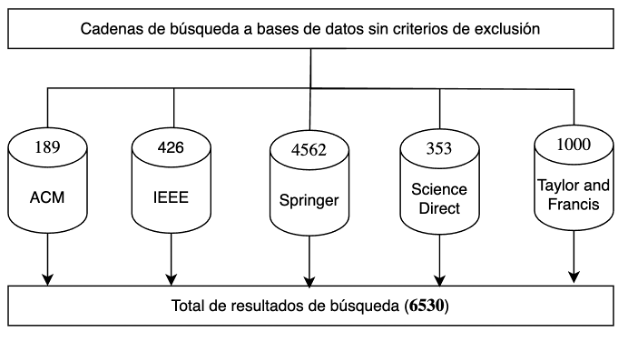
\includegraphics[scale=0.9]{tablas-images/cp2/bases-sin-criterio.png}
    \caption{Resumen de la búsqueda en bases de datos sin criterios de inclusión/exclusión}\label{fig:tabla-resumen-busqueda}
\end{figure}

\subsubsection{Métricas de la búsqueda con criterios de inclusión/exclusión}\label{subsec:resumenBusquedaCriterios}
\noindent
Esta búsqueda se realizó considerando los criterios de exclusión e inclusión definidos previamente. Las cadena de búsqueda son exactamente iguales que antes, este punto se diferencia por la aplicación de filtros. Para ver las capturas de pantalla veáse el apéndice~\ref{sec:busqueda-con-criterios}.
La Tabla~\ref{tab:bases-sin-criterio} muestra los resultados obtenidos tras aplicar los criterios de inclusión y exclusión previamente definidos. A diferencia de la búsqueda inicial, en esta fase se utilizaron filtros específicos que redujeron significativamente la cantidad de publicaciones relevantes. En total se identificaron 976 documentos, distribuidos en las bases de datos de la siguiente manera: ACM (48), IEEE (134), Springer (592), Science Direct (46) y Taylor \& Francis (156).

\begin{table}[H]
\centering
\scriptsize
\setlength{\tabcolsep}{4pt}
\renewcommand{\arraystretch}{1.1}
\begin{tabular}{|l|c|c|c|c|c|c|}
\hline
\textbf{Bases de datos} & \textbf{ACM} & \textbf{IEEE} & \textbf{Springer} & \textbf{Science Direct} & \textbf{Taylor \& Francis} & \textbf{Total} \\
\hline
Sin aplicar criterios & 189 & 426 & 4562 & 353 & 1000 & 6530 \\
\hline
Con criterios aplicados & 48 & 134 & 592 & 46 & 156 & 976 \\
\hline
\end{tabular}
\caption{Resumen de la búsqueda en bases de datos con criterios de inclusión/exclusión}\label{tab:resumen-busqueda}
\end{table}
\begin{figure}[H]
    \centering
    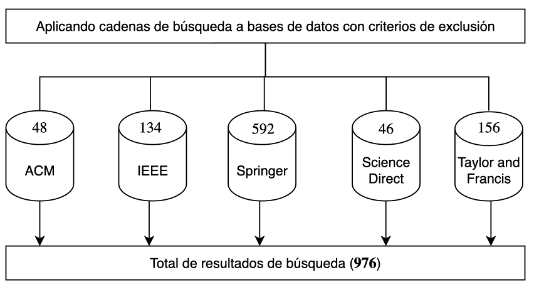
\includegraphics[scale=0.9] {tablas-images/cp2/bases-con-criterio.png}
    \caption{Resumen de la búsqueda en bases de datos con criterios de inclusión/exclusión}\label{fig:tabla-resumen-busqueda-con-criterio}
\end{figure}

\section{Eliminación de duplicados}\label{sec:eliminacionDuplicados}
\noindent
La eliminación de duplicados se realizó haciendo uso de la herramienta de gestión de referencias Mendeley. Luego de obtener los artículos se agregaron a Mendeley y esta herramienta se encargó de eliminar duplicados. En este punto se eliminaron 274 artículos duplicados.

\section{Priorización de estudios}\label{sec:priorizacionEstudios}
\noindent
Luego de la selección inicial de los artículos, se procedió a revisar el \textit{title}, \textit{abstract} y \textit{keywords} de cada uno. Como resultado de esta revisión, se generaron métricas de calidad para cada artículo, con el fin de priorizar aquellos más relevantes para la investigación. Las métricas utilizadas fueron las siguientes:

\begin{itemize}
	\item \textbf{SCI} \textit{(Science Citation Index)}
	\item \textbf{CVI} \textit{(Core Value Index)}
	\item \textbf{IRRQ} \textit{(Index Relation Research Question)}
\end{itemize}
\noindent
Este proceso inició con un total de 771 artículos, los cuales fueron evaluados según su alineamiento con los objetivos de la investigación. La evaluación temática permitió identificar un total de 110 artículos con una relación directa con el enfoque planteado.

\section{Estrategia de búsqueda usando bola de nieve}\label{sec:bolaDeNieve}
\noindent
En esta etapa, se seleccionó el primer cuartil según el índice SCI, lo que resultó en un total de 24 artículos. Adicionalmente, se incluyó un artículo por criterio de inclusión directa, estableciendo así una línea base de 25 artículos.
Partiendo de esta base, se aplicó la estrategia de bola de nieve en dos direcciones: hacia adelante y hacia atrás. Como resultado, se obtuvieron 87 artículos aplicando la técnica hacia atrás y 495 artículos aplicando la técnica hacia adelante.
Esto definió un nuevo conjunto de artículos para un proceso de selección adicional (\textit{screening}). En esta fase, se eliminaron 14 duplicados y 452 artículos fueron descartados por no aportar valor a la investigación.
Finalmente, se obtuvo un total de 116 artículos mediante esta estrategia de búsqueda.

\section{Diagrama de búsqueda}\label{sec:diagramaBusqueda}

\subsection{Usando cadenas de búsqueda}
\noindent
En el diagrama~\ref{tab:tabla-diagrama-cadena-busqueda} se puede apreciar la estrategia de búsqueda de artículos por medio de base de datos, aplicando las cadenas de búsqueda, se consolidaron los resultados de distintas bases de datos para obtener un total de 6530 resultados, posteriormente y aplicando criterios de exclusión se redujo esta cantidad a menos de 1000 resultados. Adicional a los criterios de exclusión, también se hizo eliminación de artículos duplicados, 205 por parte del ~\textit{Reference Manager}, y 69 por parte del ~\textit{SMS-Builder} para un total de 274 artículos removidos. Finalmente, se realiza la etapa de screening, donde se leen las secciones claves de los artículos, como ~\textit{abstract}, ~\textit{keywords} e introducción, a través de esto se pudo descargar 593 artículos que no eran pertinentes para el estudio.
\begin{table}[H]
    \centering
    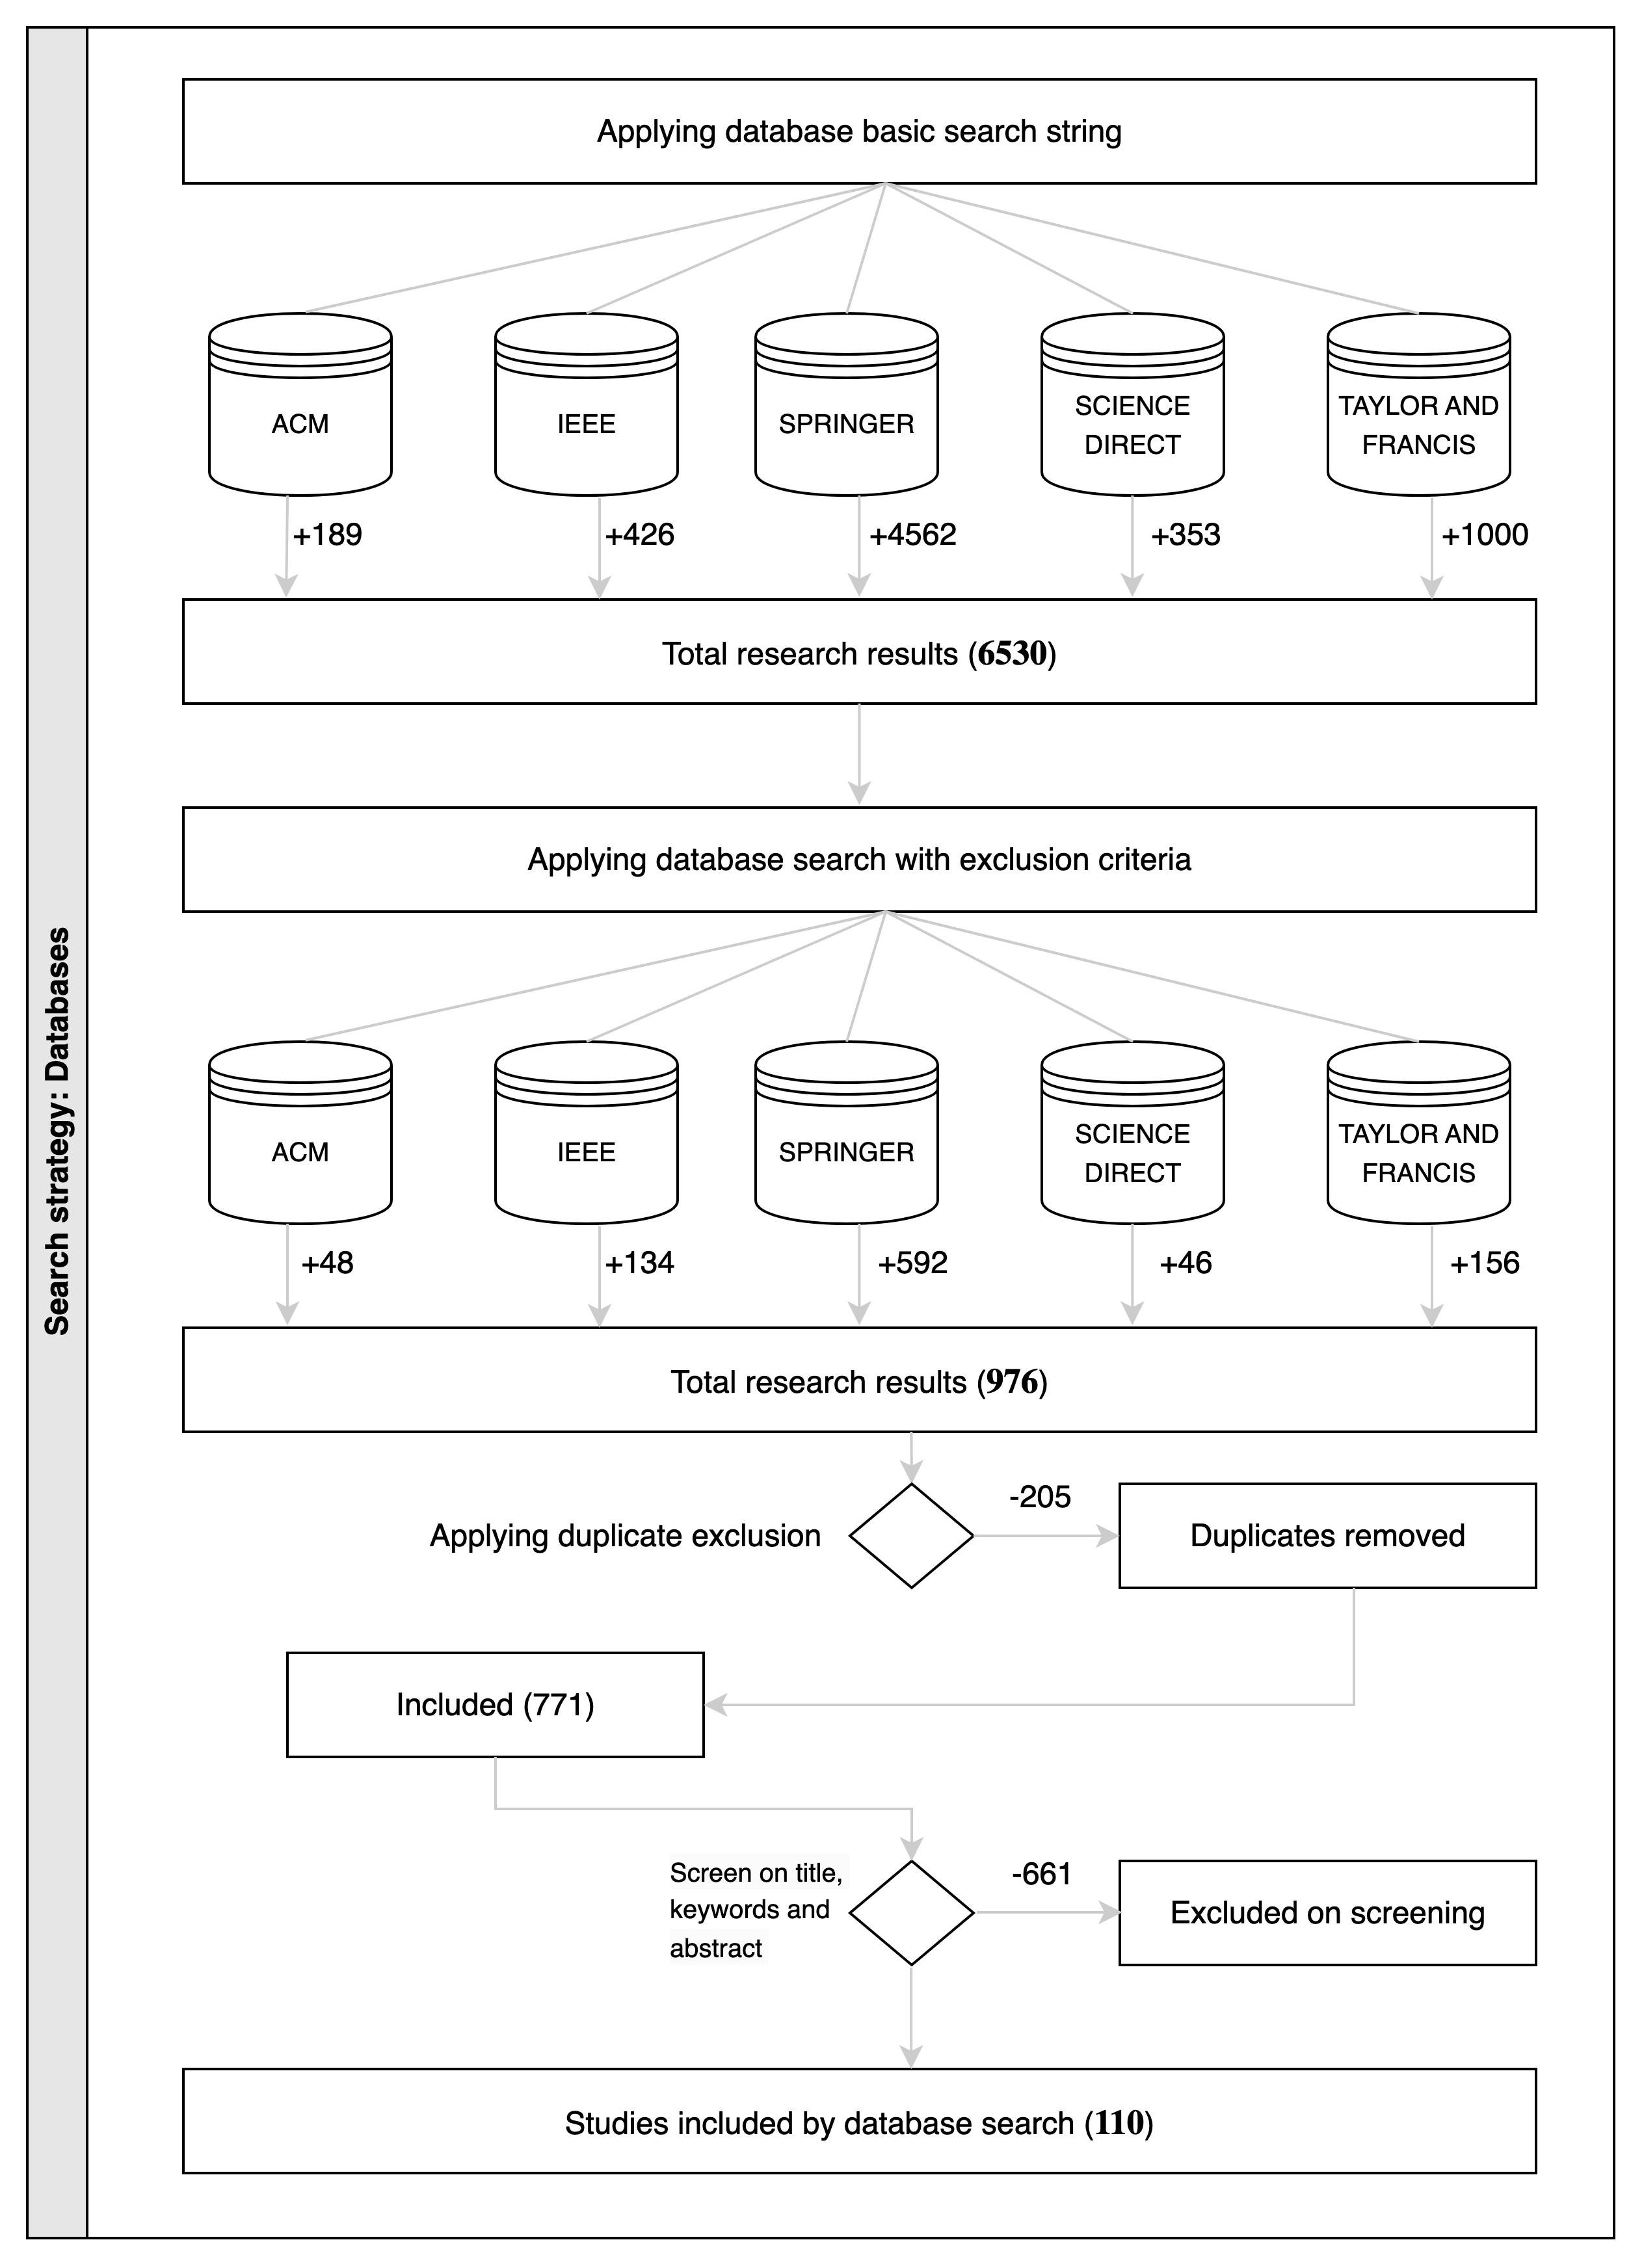
\includegraphics[scale=0.13]{tablas-images/cp2/diagrama-cadena-busqueda.png}
    \caption{Diagrama de la cadena de búsqueda}\label{tab:tabla-diagrama-cadena-busqueda}
\end{table}\label{img:busqueda-bd}

\subsection{Usando bola de nieve}
\noindent
Como segunda estrategia de búsqueda dentro del SMS, se aplicó la técnica de ~\textit{Snowball}, la cual consiste en extraer artículos adicionales a partir de las referencias citadas en los estudios obtenidos en la estrategia anterior y de los estudios que citan a estos. De los 110 estudios del paso anterior, se seleccionan aquellos que tenían un SCI más alto (primer cuartil) y se agrega uno por inclusión directa, con esto se obtiene un total de 25 artículos de línea base. Aplicando la técnica hacia adelante (artículos referenciados) se obtienen 87 nuevos estudios y la misma hacia atrás (artículos que referencian el artículo base) se obtienen 495, para un total de 582. Finalmente, se filtraron duplicados para iniciar la revisión del \textit{screening}. Como resultado 116 artículos fueron incluidos por bola de nieve. Todo este proceso se puede apreciar en la gráfica~\ref{tab:tabla-diagrama-bola-nieve-busqueda}.
\begin{table}[H]
    \centering
    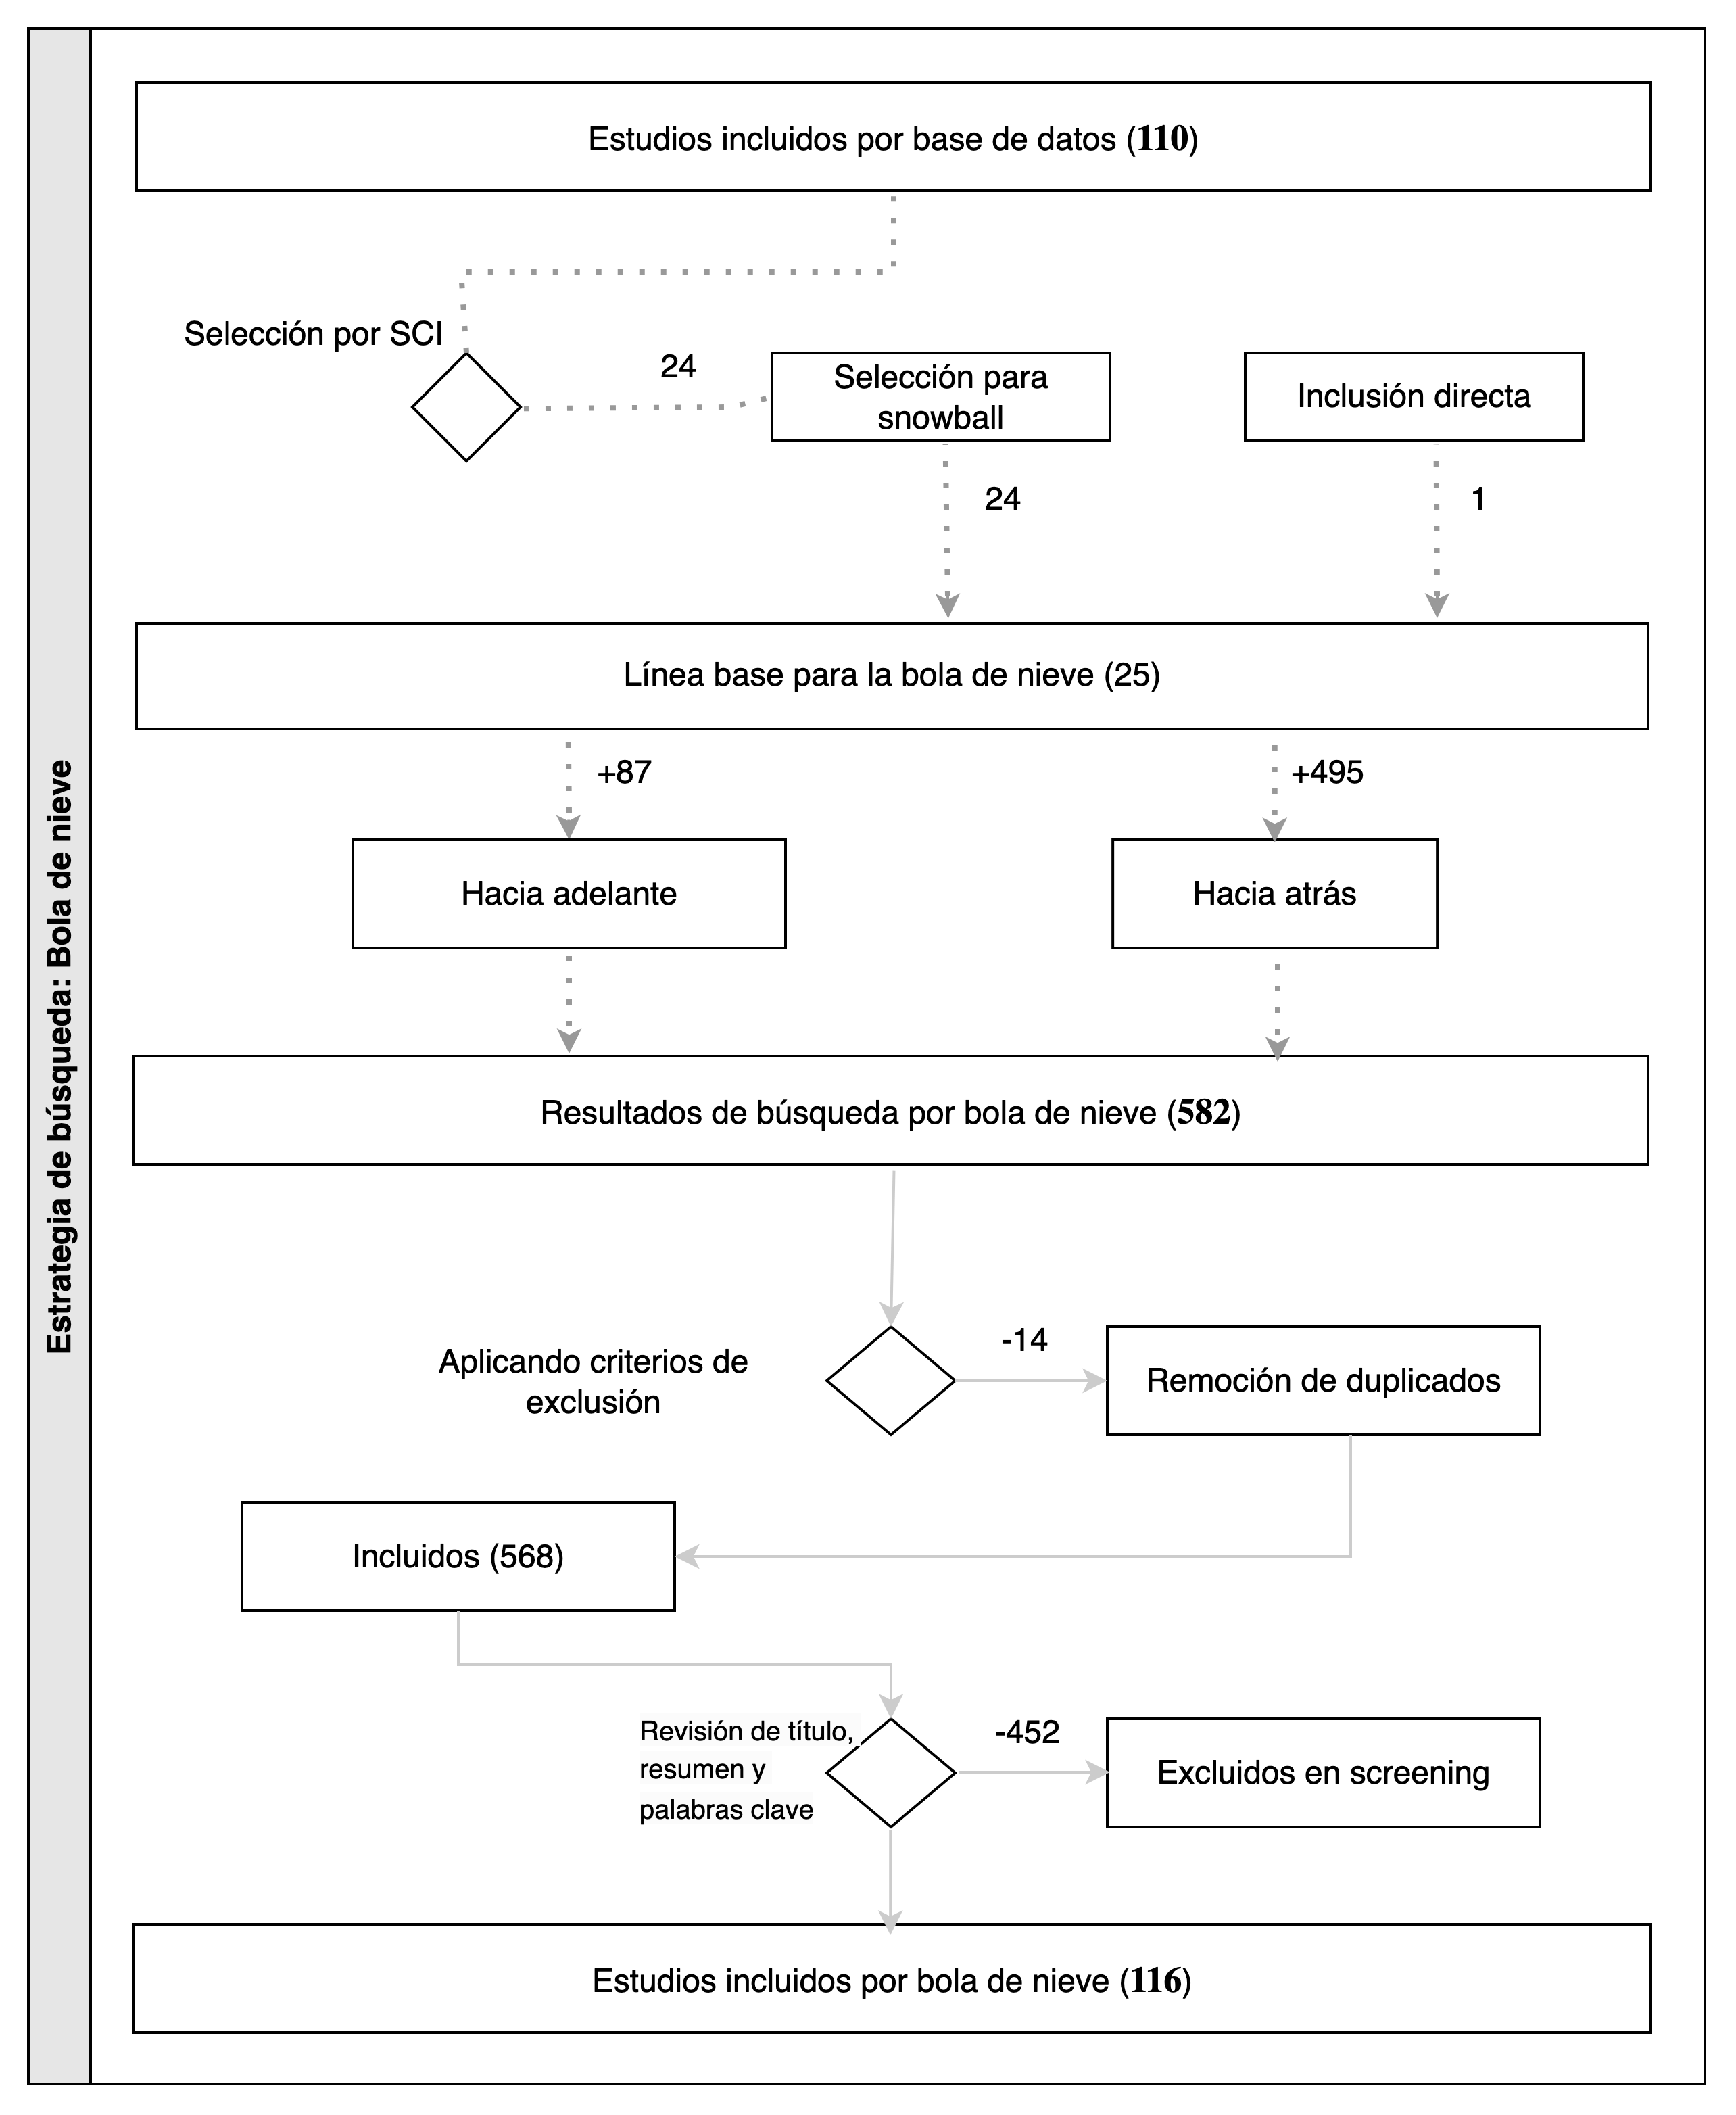
\includegraphics[scale=0.14]{tablas-images/cp2/diagrama-bola-nieve-busqueda.png}
    \caption{Diagrama de la búsqueda en bola de nieve}\label{tab:tabla-diagrama-bola-nieve-busqueda}
\end{table}

\section{Identificación de estudios}

\subsection{Artículos por año y métricas}
\noindent
A continuación se presentan las gráficas de los resultados de la búsqueda.
En la figura~\ref{fig:diagrama-articulos-ano-metrica} se pueden visualizar las métricas de calidad, separadas por los últimos 3 años y mostrando el promedio en cada métrica de los artículos publicados en esos años, así como un apartado donde se calcula la sumatoria de estas métricas por cada año.

\begin{figure}[H]
    \centering
    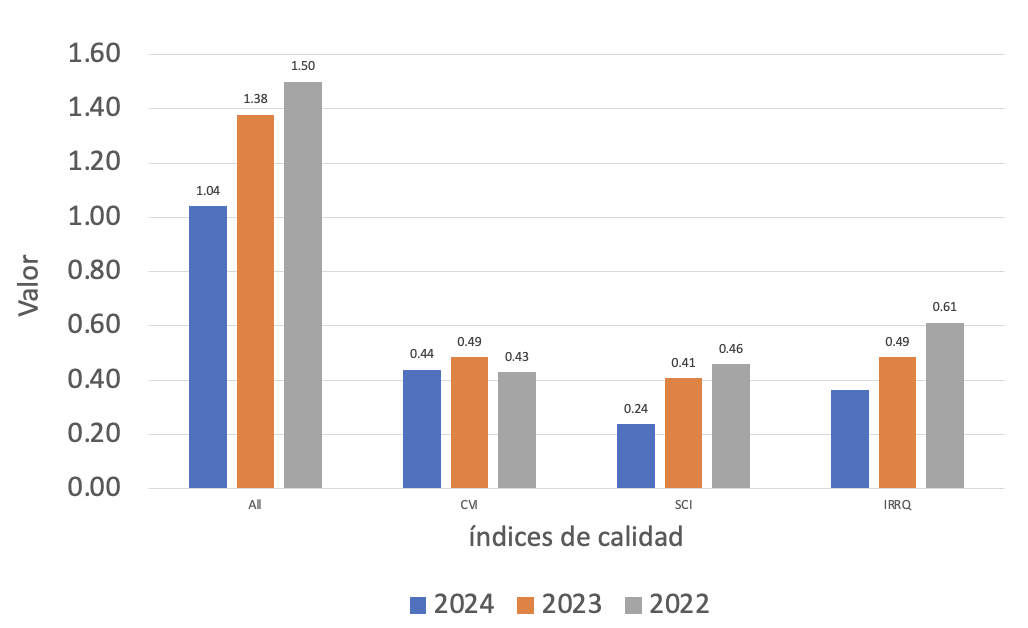
\includegraphics[scale=0.7]{tablas-images/cp2/diagrama-articulos-ano-metrica.png}
    \caption{Artículos por métricas y año}\label{fig:diagrama-articulos-ano-metrica}
\end{figure}

En la figura~\ref{fig:tipos-articulos} se muestra el conteo de artículos por su tipo específico, el cual puede ser uno de 3 opciones: 'Revista', 'Conferencia' o 'Genérico'. Vemos que la mayoría de artículos provienen de revistas.
\begin{figure}[H]
    \centering
    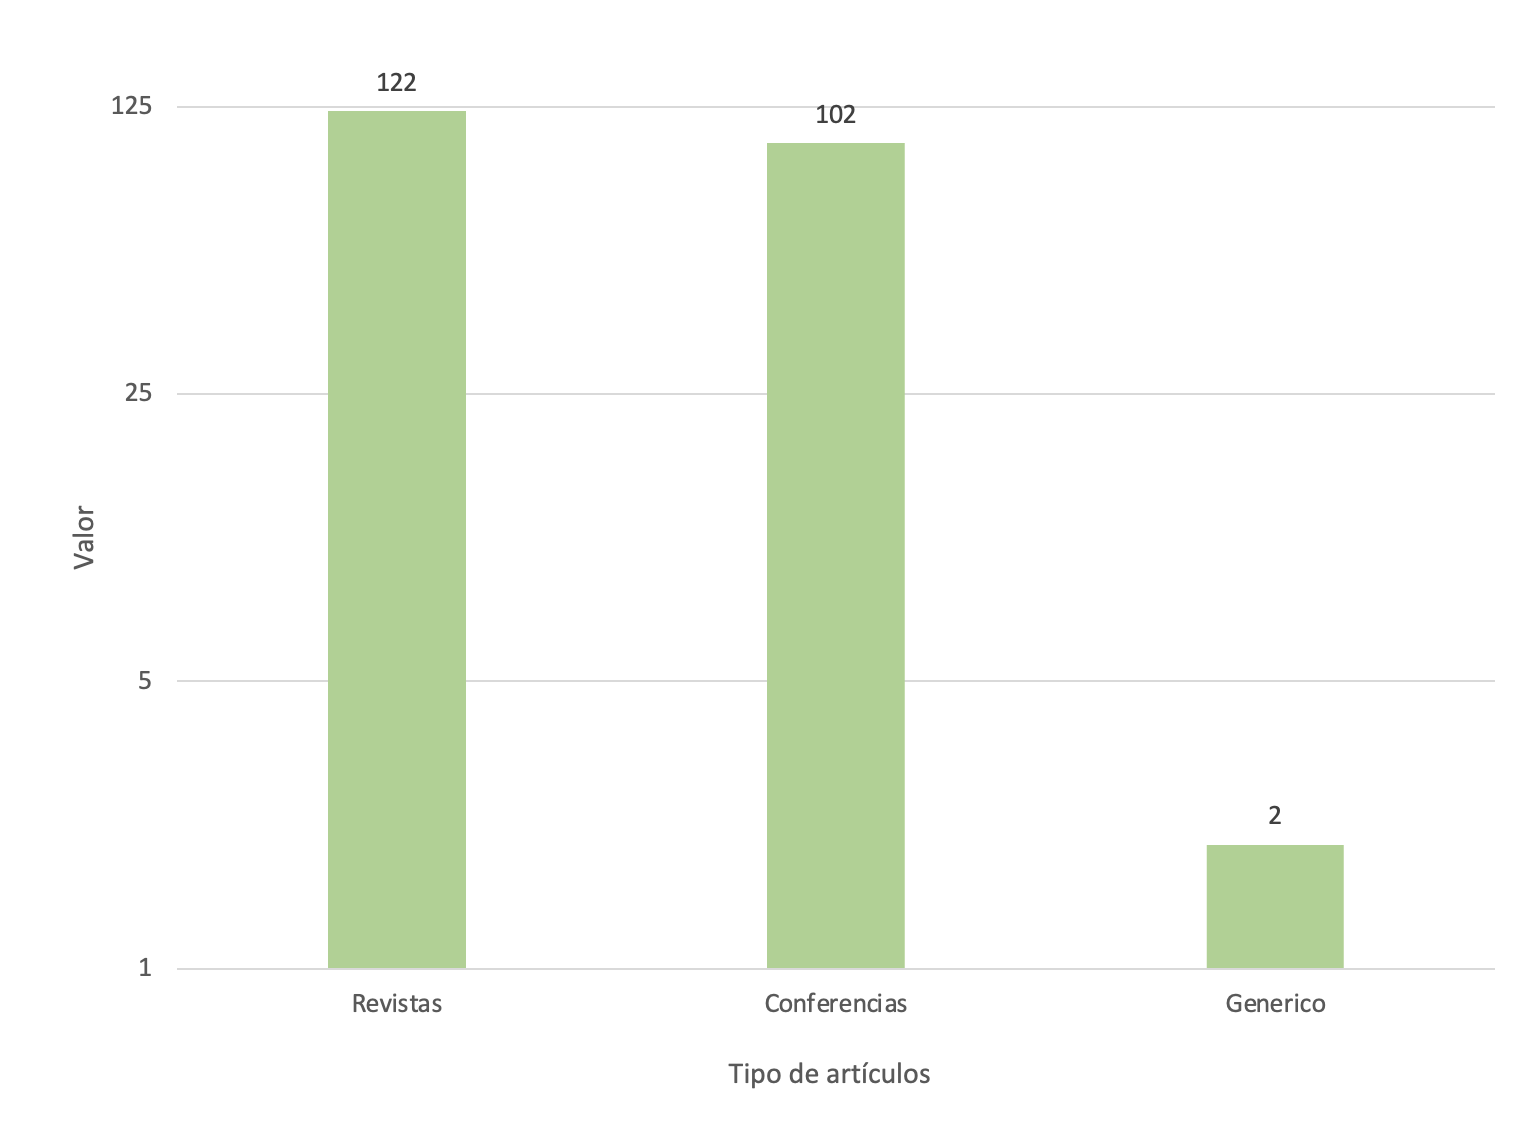
\includegraphics[scale=0.5]{tablas-images/cp2/tipos-articulos.png}
    \caption{Artículos por tipo}\label{fig:tipos-articulos}
\end{figure}

En la figura~\ref{fig:estrategia-busqueda-articulos} se detalla la cantidad de artículos que se extrajeron de cada estrategia. Se puede observar que la estrategia que generó más artículos fue la técnica de ~\textit{Snowball}.
\begin{figure}[H]
    \centering
    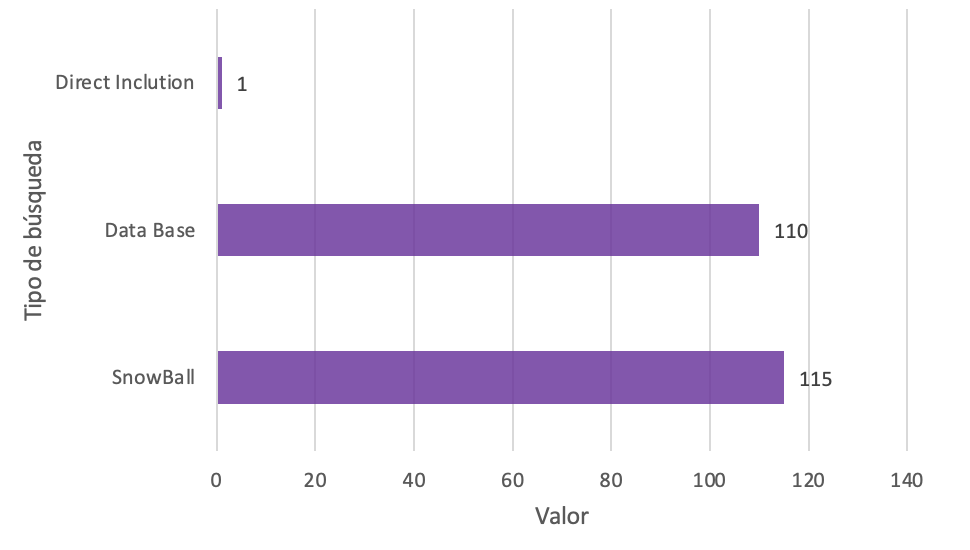
\includegraphics[scale=0.8]{tablas-images/cp2/estrategia-busqueda-articulos.png}
    \caption{Estrategia de búsqueda de artículos}\label{fig:estrategia-busqueda-articulos}
\end{figure}

Finalmente, en la figura~\ref{fig:diagrama-red-articulos} se puede apreciar un diagrama de red, que segrega por colores los tópicos más relacionados entre sí, vemos 4 grandes grupos: IA, cloud computing, virtualización, desarrollo de software.
\begin{figure}[H]
    \centering
    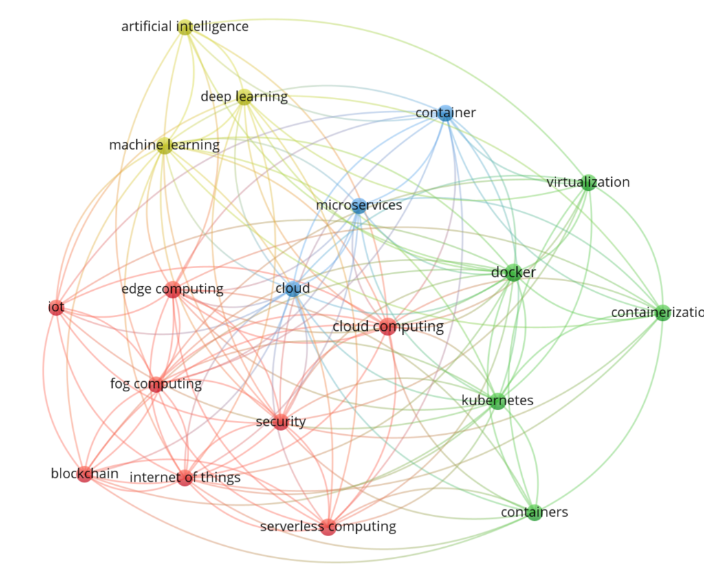
\includegraphics[scale=0.9]{tablas-images/cp2/diagrama-red-busqueda.png}
    \caption{Diagrama de red de los artículos}\label{fig:diagrama-red-articulos}
\end{figure}

\section{Identificación de tecnologías de \VBC}\label{sec:tecnologias-vbc-identificadas}
\noindent
En esta sección se presentan las tecnologías de \VBC\ y las tecnologías de orquestación identificadas en el proceso de revisión sistemática de la literatura. \\
\noindent
El gráfico presentado en la Figura~\ref{fig:tecnologias-vbc} expone la distribución de las tecnologías de \VBC\ identificadas en el estudio de mapeo sistemático. En él se observa que Docker es la tecnología con mayor representación, acumulando 94 menciones, lo que evidencia su posición dominante en el ecosistema. En contraste, alternativas como Podman, LXC y Containerd muestran una presencia moderada, mientras que tecnologías como OpenVZ y Hyper-V containers apenas alcanzan una mención. Este comportamiento refleja tanto la consolidación de Docker como estándar \textit{de facto} en el ámbito de los contenedores, como la coexistencia de múltiples soluciones que, aunque menos extendidas, representan enfoques relevantes para casos de uso específicos. \\
\input{tablas-images/cp2/tecnologias-vbc.tex}
\noindent
La Figura~\ref{fig:tecnologias-orquestacion} muestra la distribución de las tecnologías de orquestación identificadas en el estudio de mapeo sistemático. El gráfico evidencia una clara predominancia de Kubernetes, con 67 menciones, consolidándose como la solución de referencia en la gestión de contenedores. En un segundo nivel, tecnologías como Docker Swarm (9) y Apache Mesos (5) presentan una adopción moderada, mientras que opciones como OpenShift, Docker Compose, Amazon ECS y Amazon EKS aparecen con una menor representación. Estos resultados reflejan la consolidación de Kubernetes como estándar en orquestación, a la vez que destacan la diversidad de alternativas que, aunque menos extendidas, atienden necesidades específicas en determinados contextos.
\input{tablas-images/cp2/tecnologias-orquestacion.tex}

\section{Información de la herramienta}

\noindent
La herramienta utilizada para este proceso de revisión de la literatura fue \textbf{SMS-BUILDER}, la cual se encuentra disponible en \textit{Docker Hub}. La imagen puede consultarse en el siguiente enlace:

\begin{center}
	\href{https://hub.docker.com/r/griduq/sms-builder}{\texttt{https://hub.docker.com/r/griduq/sms-builder}}
\end{center}



\section{Reproducibilidad del método}
\noindent
Con el fin de fomentar la reproducibilidad del método de revisión, se proporcionan dos mecanismos de verificación que permiten a los revisores y lectores acceder de forma transparente a la información utilizada, generada mediante la herramienta SMS-Builder de~\cite{SMSBuilder2020}
\begin{itemize}
	\item Un enlace de acceso público a la instancia de SMS-Builder que contiene todos los datos del proceso de revisión sistemática: \href{https://sms-vbc.iti.grid.uniquindio.edu.co/sms.xhtml}{link}. Las credenciales de acceso son ``invitado'' tanto para el nombre de usuario como para la contraseña.
	\item Una imagen de Docker de acceso público que integra toda la documentación necesaria para crear un contenedor con los datos del proceso: \href{https://hub.docker.com/r/anubis1001/tg-vbc-sms-builder}{link}.
\end{itemize}

\noindent
Adicionalmente, se implementaron procesos de respaldo como medida de seguridad. Estos \textit{backups} fueron almacenados en ubicaciones diferentes, siguiendo la estrategia de respaldo \textbf{3--2--1}.

\section{Conclusiones de la revisión sistemática de la literatura}
\noindent
Esta sección presenta un mapeo sistemático de la literatura sobre tecnologías de virtualización basadas en contenedores, principalmente relacionada con la educación, la investigación y la extensión. Dentro del \SMS, se definió un esquema de clasificación según los temas específicos establecidos durante la fase de planificación. Este esquema proporciona un mapeo de la información en tablas y gráficos estadísticos que ayudan a describir los datos y su relación con las preguntas de investigación. El mapeo sistemático reveló una creciente proliferación de estudios relacionados con las tecnologías de \VBC, incluyendo estudios en diferentes áreas y aplicaciones. Esta proliferación de estudios podría ser contraproducente para ciertas partes interesadas a la hora de implementar arquitecturas con estas tecnologías. Además, puede provocar una saturación de la literatura y dificultar el desarrollo, principalmente debido al abrumador volumen de información disponible. Más allá de los resultados obtenidos en este \SMS, los estudios se analizaron explorando la información subyacente y las tendencias. De este modo, se identificó una creciente adopción de la virtualización ligera en la implementación de soluciones, con especial énfasis en la computación en la nube y orquestadores como Kubernetes. Este liderazgo se ve reforzado por la necesidad de las organizaciones de proporcionar redundancia, fiabilidad y escalabilidad en sus aplicaciones y servicios.

%\section{Nichos de mercado}

\subsection{Docker}
Docker se posiciona principalmente en el nicho de mercado de desarrolladores de software, empresas tecnológicas y proveedores de servicios en la nube que buscan una solución para la creación, implementación y gestión de aplicaciones en contenedores \citep{Hill2025}. Su capacidad de automatizar despliegues y garantizar la portabilidad entre entornos lo convierte en una opción ideal para DevOps y desarrollo ágil \citep{Mag2025}.

\subsection{Podman}
Podman está orientado a entornos empresariales y desarrolladores que requieren una solución de contenerización sin \textit{daemon}, compatible con OCI y con enfoque en la seguridad \citep{Surendhar2024}. Su naturaleza sin \textit{daemon} y su capacidad para ejecutar contenedores de forma aislada permiten su adopción en entornos donde la seguridad y la conformidad son prioridades \citep{Trevor2022}.

\subsection{Udocker}
Udocker se especializa en nichos de mercado académicos y de investigación, donde los usuarios necesitan ejecutar contenedores sin privilegios en sistemas que no permiten la instalación de software de nivel de sistema \citep{Campos2017}. Su facilidad para funcionar en entornos HPC (Computación de Alto Rendimiento) sin requerir permisos de root lo hace adecuado para instituciones de investigación \citep{Gomes2018}.

\subsection{Wasm (WebAssembly)}
Wasm se centra en el nicho de desarrollo web y aplicaciones de alto rendimiento en el navegador \citep{Haas2017}. Su capacidad para ejecutar código de forma eficiente en múltiples plataformas, incluidas aplicaciones de escritorio y móviles, lo convierte en una opción atractiva para empresas de desarrollo de software que buscan optimización multiplataforma \citep{Jangda2019}.

\subsection{LXC (Linux Containers)}
LXC es popular en entornos de virtualización ligera y servidores, donde se requiere un control granular sobre los entornos de contenedores \citep{Silva2024}. Su uso está orientado a proveedores de alojamiento web, desarrolladores de software y administradores de sistemas que necesitan un control preciso del entorno del sistema operativo \citep{Simon2023}.

\subsection{Containerd}
Containerd está dirigido a proveedores de servicios en la nube y plataformas de orquestación como Kubernetes, donde se requiere una solución de gestión de contenedores ligera y compatible con OCI \citep{Vano2023}. Su arquitectura modular lo convierte en una opción preferida para grandes infraestructuras \citep{Zhou2021}.

\subsection{LXD}
LXD se enfoca en nichos de mercado que requieren entornos de virtualización basados en contenedores que imiten máquinas virtuales, como proveedores de servicios en la nube, plataformas de pruebas y entornos de desarrollo \citep{Silva2024}. Su capacidad para ofrecer entornos de sistema completo lo hace ideal para desarrolladores y administradores de sistemas \citep{Kaiser2022}.

\subsection{Rkt}
Rkt fue diseñado para satisfacer las necesidades de proveedores de servicios en la nube y organizaciones que buscan una alternativa a Docker con un enfoque en la seguridad y compatibilidad OCI \citep{Lingayat2018}. Aunque su desarrollo ha sido discontinuado, sigue siendo relevante en entornos donde la compatibilidad y la seguridad son críticas \citep{Watada2019}.

\subsection{Singularity}
Singularity se centra en entornos de computación científica y HPC, donde se requiere portabilidad de aplicaciones sin necesidad de privilegios de root \citep{10.1145/3332186.3332192}. Es ampliamente adoptado en universidades, centros de investigación y laboratorios que ejecutan aplicaciones de alto rendimiento \citep{Kurtzer2017}.

\subsection{runC}
runC está orientado a proveedores de servicios en la nube, plataformas de orquestación como Kubernetes y desarrolladores de software que buscan una solución de contenedorización ligera y compatible con OCI \citep{Perez2005}. Su adopción en proyectos de gran escala se debe a su eficiencia y cumplimiento de estándares de contenedores \citep{151962df5f7e4b9faba0629540c11439}.

\subsection{CRI-O}
CRI-O está diseñado específicamente para su integración con Kubernetes, sirviendo como un motor de contenedores ligero y compatible con OCI para esta plataforma \citep{CNCF2019}. Es una solución ideal para proveedores de servicios en la nube y organizaciones que utilizan Kubernetes como su plataforma de orquestación principal \citep{151962df5f7e4b9faba0629540c11439}.

\subsection{Hyper-V Containers}
Hyper-V Containers están orientados a empresas que utilizan infraestructuras basadas en Windows, ofreciendo una solución de contenedorización segura y eficiente para aplicaciones basadas en Windows \citep{Smith2016}. Su integración con el ecosistema de Microsoft lo hace ideal para empresas con infraestructuras híbridas \citep{Clark2024}.

\subsection{OpenVZ}
OpenVZ se centra en proveedores de alojamiento web y servicios VPS, donde se requiere una solución de virtualización ligera basada en contenedores que permita un control granular sobre los recursos del sistema y la administración de múltiples instancias \citep{OpenVZ2015}.

\subsection{Linux VServer}
Linux VServer está orientado a administradores de sistemas y proveedores de servicios que requieren una solución de virtualización ligera basada en contenedores para la administración de servidores seguros y eficientes \citep{10.1145/1272996.1273025}. Es una opción adecuada para entornos de servidor dedicados y alojamientos compartidos \citep{LinuxVirt2017}.

\subsection{Google gVisor}
Google gVisor está dirigido a proveedores de servicios en la nube y organizaciones que priorizan la seguridad en sus entornos de contenedores \citep{LopezFalcon2024}. Su arquitectura de \textit{sandbox} proporciona un aislamiento fuerte, lo que lo convierte en una opción atractiva para aplicaciones sensibles \citep{gvisor2025}.

\subsection{Kata Containers}
Kata Containers se centra en entornos donde se requiere un alto nivel de seguridad y aislamiento, como proveedores de servicios en la nube y empresas que manejan información confidencial \citep{Viktorsson2020}. Su capacidad para combinar la eficiencia de los contenedores con el aislamiento de máquinas virtuales es su principal ventaja \citep{10.1145/1272996.1273025}.

\subsection{Firecracker}
Firecracker está orientado a proveedores de servicios en la nube y plataformas de cómputo en la nube que requieren micro VMs eficientes y seguras \citep{Jain}. Es una solución ideal para plataformas \textit{serverless} y entornos multi-tenant \citep{246288}.

\subsection{Sarus}
Sarus está dirigido a entornos de HPC y computación científica, donde los usuarios necesitan ejecutar contenedores de forma segura en sistemas de alto rendimiento \citep{Sarus2021}. Su compatibilidad con estándares de contenedores y su enfoque en la seguridad lo hacen ideal para centros de investigación y universidades \citep{B2020}.


\begin{table}[H]
\centering
\scriptsize
\setlength{\tabcolsep}{3pt}
\renewcommand{\arraystretch}{1.1}
\begin{tabular}{|>{\centering\arraybackslash}m{0.18\textwidth}| 
                >{\centering\arraybackslash}m{0.25\textwidth}| 
                >{\centering\arraybackslash}m{0.20\textwidth}| 
                >{\centering\arraybackslash}m{0.25\textwidth}|}
\hline
\textbf{Tecnologías} & \textbf{Licencias} & \textbf{Términos de uso} & \textbf{Costo} \\
\hline
Docker & Apache 2.0 & \href{https://www.docker.com/legal/docker-terms-service/}{link} & \$11-\$24 \\
\hline
Podman & Apache 2.0 & \href{https://github.com/containers/podman/blob/main/LICENSE}{link} & Gratis \\
\hline
Udocker & Apache 2.0 & \href{https://github.com/indigo-dc/udocker/blob/master/LICENSE}{link} & Gratis \\
\hline
Wasm & Apache 2.0 & \href{https://github.com/WebAssembly/design/blob/main/LICENSE}{link} & Gratis \\
\hline
LXC & GNU LGPLv2.1+ & \href{https://linuxcontainers.org/lxc/introduction/}{link} & Gratis \\
\hline
Containerd & Apache 2.0 & \href{https://github.com/containerd/containerd/blob/main/LICENSE}{link} & Gratis \\
\hline
LXD & AGPL-3.0 & \href{https://github.com/canonical/lxd}{link} & Gratis \\
\hline
Rkt & Apache 2.0 & \href{https://github.com/rkt/rkt/blob/master/LICENSE}{link} & Descontinuado \\
\hline
Singularity & BSD 3-Clause & \href{https://github.com/sylabs/singularity/blob/main/LICENSE.md}{link} & CE: Gratis, PRO: \$30/año \\
\hline
runC & Apache 2.0 & \href{https://github.com/opencontainers/runc/blob/main/LICENSE}{link} & Gratis \\
\hline
CRI-O & Apache 2.0 & \href{https://github.com/cri-o/cri-o/blob/main/LICENSE}{link} & Gratis \\
\hline
Hyper-V containers & Windows Propietaria & \href{https://learn.microsoft.com/es-es/virtualization/windowscontainers/images-eula}{link} & \$1,176 USD \\
\hline
OpenVZ & GPL v2 & \href{https://openvz.org/}{link} & Gratis \\
\hline
Linux VServer & GPL v2 & \href{http://linux-vserver.org/}{link} & Gratis \\
\hline
Google gVisor & Apache 2.0 & \href{https://github.com/google/gvisor}{link} & Gratis \\
\hline
Kata Containers & Apache 2.0 & \href{https://github.com/kata-containers/kata-containers/blob/main/LICENSE}{link} & Gratis \\
\hline
Firecracker & Apache 2.0 & \href{https://github.com/firecracker-microvm/firecracker}{link} & Gratis \\
\hline
Sarus & BSD 3-Clause & \href{https://github.com/eth-cscs/sarus}{link} & Gratis \\
\hline
\end{tabular}
\caption{Comparativa de tecnologías de contenerización, licencias, términos de uso y costos}
\end{table}

En la tabla~\ref{tab:interfaz-vbc} se puede ver la interfaz de uso por cada tecnología. Como se puede apreciar, la gran mayoría de tecnologías se utilizan a través de una CLI (línea de comandos). Esto, en muchos casos, puede implicar un aumento en la curva de aprendizaje, pero mayor facilidad para gestionar y automatizar las tecnologías una vez que se ha comprendido el uso de su interfaz.
\begin{table}[H]
\centering
\scriptsize
\setlength{\tabcolsep}{3pt}
\renewcommand{\arraystretch}{1.1}
\begin{tabularx}{\textwidth}{|p{0.18\textwidth}|>{\raggedright\arraybackslash}X|}
\hline
\textbf{Tecnología} & \textbf{Interfaz de Uso} \\
\hline
Docker & \CLI\ principalmente, con Docker Desktop para interfaz gráfica. \\
\hline
Podman & \CLI\ similar a Docker, sin daemon. Opcional Podman Desktop. \\
\hline
Udocker & \CLI\ específica para ejecutar contenedores sin privilegios root. \\
\hline
Wasm  & Ejecución través de navegadores web, \API\ de JavaScript. \\
\hline
LXC & \CLI\ mediante comando lxc, sin interfaz gráfica oficial. \\
\hline
Containerd & \CLI\ con herramientas como ctr, backend para otras herramientas. \\
\hline
LXD & \CLI\ mediante lxd/lxc, con interfaz web LXD Web \UI. \\
\hline
Rkt & \CLI\ mediante comandos como rkt run (descontinuado). \\
\hline
Singularity & \CLI\ mediante comandos singularity para gestión de contenedores. \\
\hline
runC & \CLI\ mediante comandos runc, runtime bajo Docker y Kubernetes. \\
\hline
CRI-O & \CLI, interactúa con Kubernetes, sin interfaz gráfica dedicada. \\
\hline
Hyper-V containers & \CLI\ (PowerShell) o Hyper-V Manager para \VM . \\
\hline
OpenVZ & \CLI\ mediante comandos vzctl, con interfaces gráficas de terceros. \\
\hline
Linux VServer & \CLI\ mediante comandos vserver para gestión. \\
\hline
Google gVisor & \CLI\ mediante comandos estándar de Docker con seguridad adicional. \\
\hline
Kata Containers & \CLI\ mediante kata-runtime, integración con Kubernetes. \\
\hline
Firecracker & \CLI\ mediante \API\ RESTful y herramientas firecracker. \\
\hline
Sarus & \CLI\ mediante comando sarus para entornos \HPC. \\
\hline
\end{tabularx}
\caption{Interfaz de uso de cada VBC}\label{tab:interfaz-vbc}
\end{table}

En el cuadro~\ref{tab:integracion-cloud-vbc} se puede ver la integración a las distintas plataformas cloud que tiene cada tecnología. Se puede ver que muchas tecnologías tienen integración directa con 3 de los proveedores cloud más famosos, a saber: AWS, GCP y Azure. Algunas tecnologías, por otro lado, solo soportan implementación de nubes privadas, como LXD.
\begin{table}[H]
\centering
\scriptsize
\setlength{\tabcolsep}{3pt}
\renewcommand{\arraystretch}{1.1}
\begin{tabularx}{\textwidth}{|p{0.2\textwidth}|X|}
\hline
\textbf{Tecnología} & \textbf{Integración con Proveedores de Cloud} \\
\hline
Docker & Integración con \AWS\ (ECR, ECS), Google Cloud (GCR, GKE), Azure (ACR, AKS), y otros proveedores a través de herramientas como Docker Compose, Docker Swarm y Docker Desktop. \\
\hline
Podman & Compatible con \AWS\ (ECR), Google Cloud (GCR), Azure (ACR), aunque su integración con orquestadores como Kubernetes es más reciente y menos prevalente que Docker. \\
\hline
Udocker & Generalmente se usa en entornos sin privilegios de root y en plataformas como \HPC\ . No tiene una integración directa con proveedores de nube a gran escala. \\
\hline
Wasm (WebAssembly) & Integración principalmente con servicios de computación en la nube como \AWS\ Lambda, Google Cloud Functions, y Azure Functions, ya que permite la ejecución eficiente de código en la nube sin dependencia del sistema operativo subyacente. \\
\hline
LXC & Se puede integrar en plataformas de nube privada y algunas soluciones híbridas. Se usa en servidores de nube como OpenStack, pero no tiene una integración directa con plataformas públicas principales. \\
\hline
Containerd & Integración fuerte con Kubernetes, que a su vez se integra con proveedores de nube como \AWS\ (EKS), Google Cloud (GKE), Azure (AKS) y otros. \\
\hline
LXD & Puede integrarse con plataformas de nube privada, como OpenStack, para ofrecer contenedores ligeros que emulan máquinas virtuales. No tiene integración directa con los proveedores de nube pública principales, pero puede ser utilizado en soluciones personalizadas. \\
\hline
Rkt & Aunque estaba integrado con Kubernetes y otras plataformas, su descontinuación limita la integración con proveedores de nube. En el pasado, soportaba plataformas como \AWS\ y Google Cloud. \\
\hline
Singularity & Utilizado principalmente en entornos de computación científica y HPC. Puede integrarse con proveedores como \AWS\ (HPC, Batch) y Google Cloud (Compute Engine) para tareas específica de alto rendimiento. \\
\hline
runC & Integración con Kubernetes, que se usa ampliamente en proveedores de nube como \AWS\ (EKS), Google Cloud (GKE), y Azure (AKS) para la orquestación de contenedores. \\
\hline
CRI-O & Integración directa con Kubernetes, lo que le permite ser utilizado en proveedores de nube como \AWS\ (EKS), Google Cloud (GKE), Azure (AKS), y otros servicios de orquestación de contenedores. \\
\hline
Hyper-V containers & Integración exclusiva con Microsoft Azure, especialmente con Azure Kubernetes Service (AKS) y otras soluciones basadas en Hyper-V. \\
\hline
OpenVZ & Tradicionalmente usado en proveedores de hosting como OVH, aunque su uso ha disminuido frente a soluciones más modernas. La integración con nubes públicas es limitada y generalmente personalizada. \\
\hline
Linux VServer & Utilizado principalmente en proveedores de hosting dedicados y servidores privados, sin integración directa con proveedores de nube pública como \AWS\, Google Cloud o Azure. \\
\hline
Google gVisor & Integración con Google Cloud, especialmente en Google Kubernetes Engine (GKE), para agregar una capa adicional de seguridad a los contenedores. \\
\hline
Kata Containers & Soporta proveedores de nube pública como \AWS\, Google Cloud, y Azure a través de Kubernetes, proporcionando aislamiento similar a máquinas virtuales en entornos de contenedores. \\
\hline
\end{tabularx}
\caption{Integración cloud de cada VBC}
\label{tab:integracion-cloud-vbc}
\end{table}

\section{Cuadrante Gartner}
Para visualizar el panorama de las tecnologias de contenerización en cuanto a su relevancia en la industria, se aplicó un cuadrante gartner, el cual mide dos dimensiones, Visión y Ejecución, es decir que tan buena proyeccion puede tener la tecnologia en el futuro y que tan bien se desempeña actualmente en el corto plazo.

\begin{table}[H]
\centering
\scriptsize
\setlength{\tabcolsep}{4pt}
\renewcommand{\arraystretch}{1.0}
\begin{tabular}{|p{0.3\textwidth}|c|c|p{0.25\textwidth}|}
\hline
\textbf{Tecnología} & \textbf{Visión (X)} & \textbf{Ejecución (Y)} & \textbf{Cuadrante} \\
\hline
Docker & 9 & 9 & Líderes \\
\hline
Containerd & 8 & 8 & Líderes \\
\hline
Podman & 8 & 7 & Retadores \\
\hline
CRI-O & 7 & 7 & Retadores \\
\hline
LXC & 6 & 6 & Jugadores de Nicho \\
\hline
LXD & 6 & 6 & Jugadores de Nicho \\
\hline
Udocker & 4 & 4 & Jugadores de Nicho \\
\hline
runC & 5 & 5 & Jugadores de Nicho \\
\hline
Rkt & 3 & 4 & Jugadores de Nicho \\
\hline
Singularity & 5 & 4 & Visionarios \\
\hline
Wasm & 9 & 5 & Visionarios \\
\hline
Google gVisor & 8 & 6 & Visionarios \\
\hline
Kata Containers & 7 & 6 & Visionarios \\
\hline
Firecracker & 8 & 6 & Visionarios \\
\hline
Sarus & 4 & 4 & Jugadores de Nicho \\
\hline
Hyper-V containers & 5 & 5 & Jugadores de Nicho \\
\hline
OpenVZ & 4 & 5 & Jugadores de Nicho \\
\hline
Linux VServer & 3 & 4 & Jugadores de Nicho \\
\hline
\end{tabular}
\caption{Tabla de medición para el cuadrante gartner}
\label{tab:cuadrante-gartner}
\end{table}

Una vez hecha la tabla anterior, se pueden resumir los resultados en el diagrama~\ref{fig:tabla-cuadrante-gartner}, que representa el cuadrante Gartner. Se pueden ver 4 grandes grupos de tecnologías dependiendo de su nivel de visión y ejecución: Líderes, Retadores, Visionarios, Jugadores de nicho.
\begin{figure}[H]
    \centering
    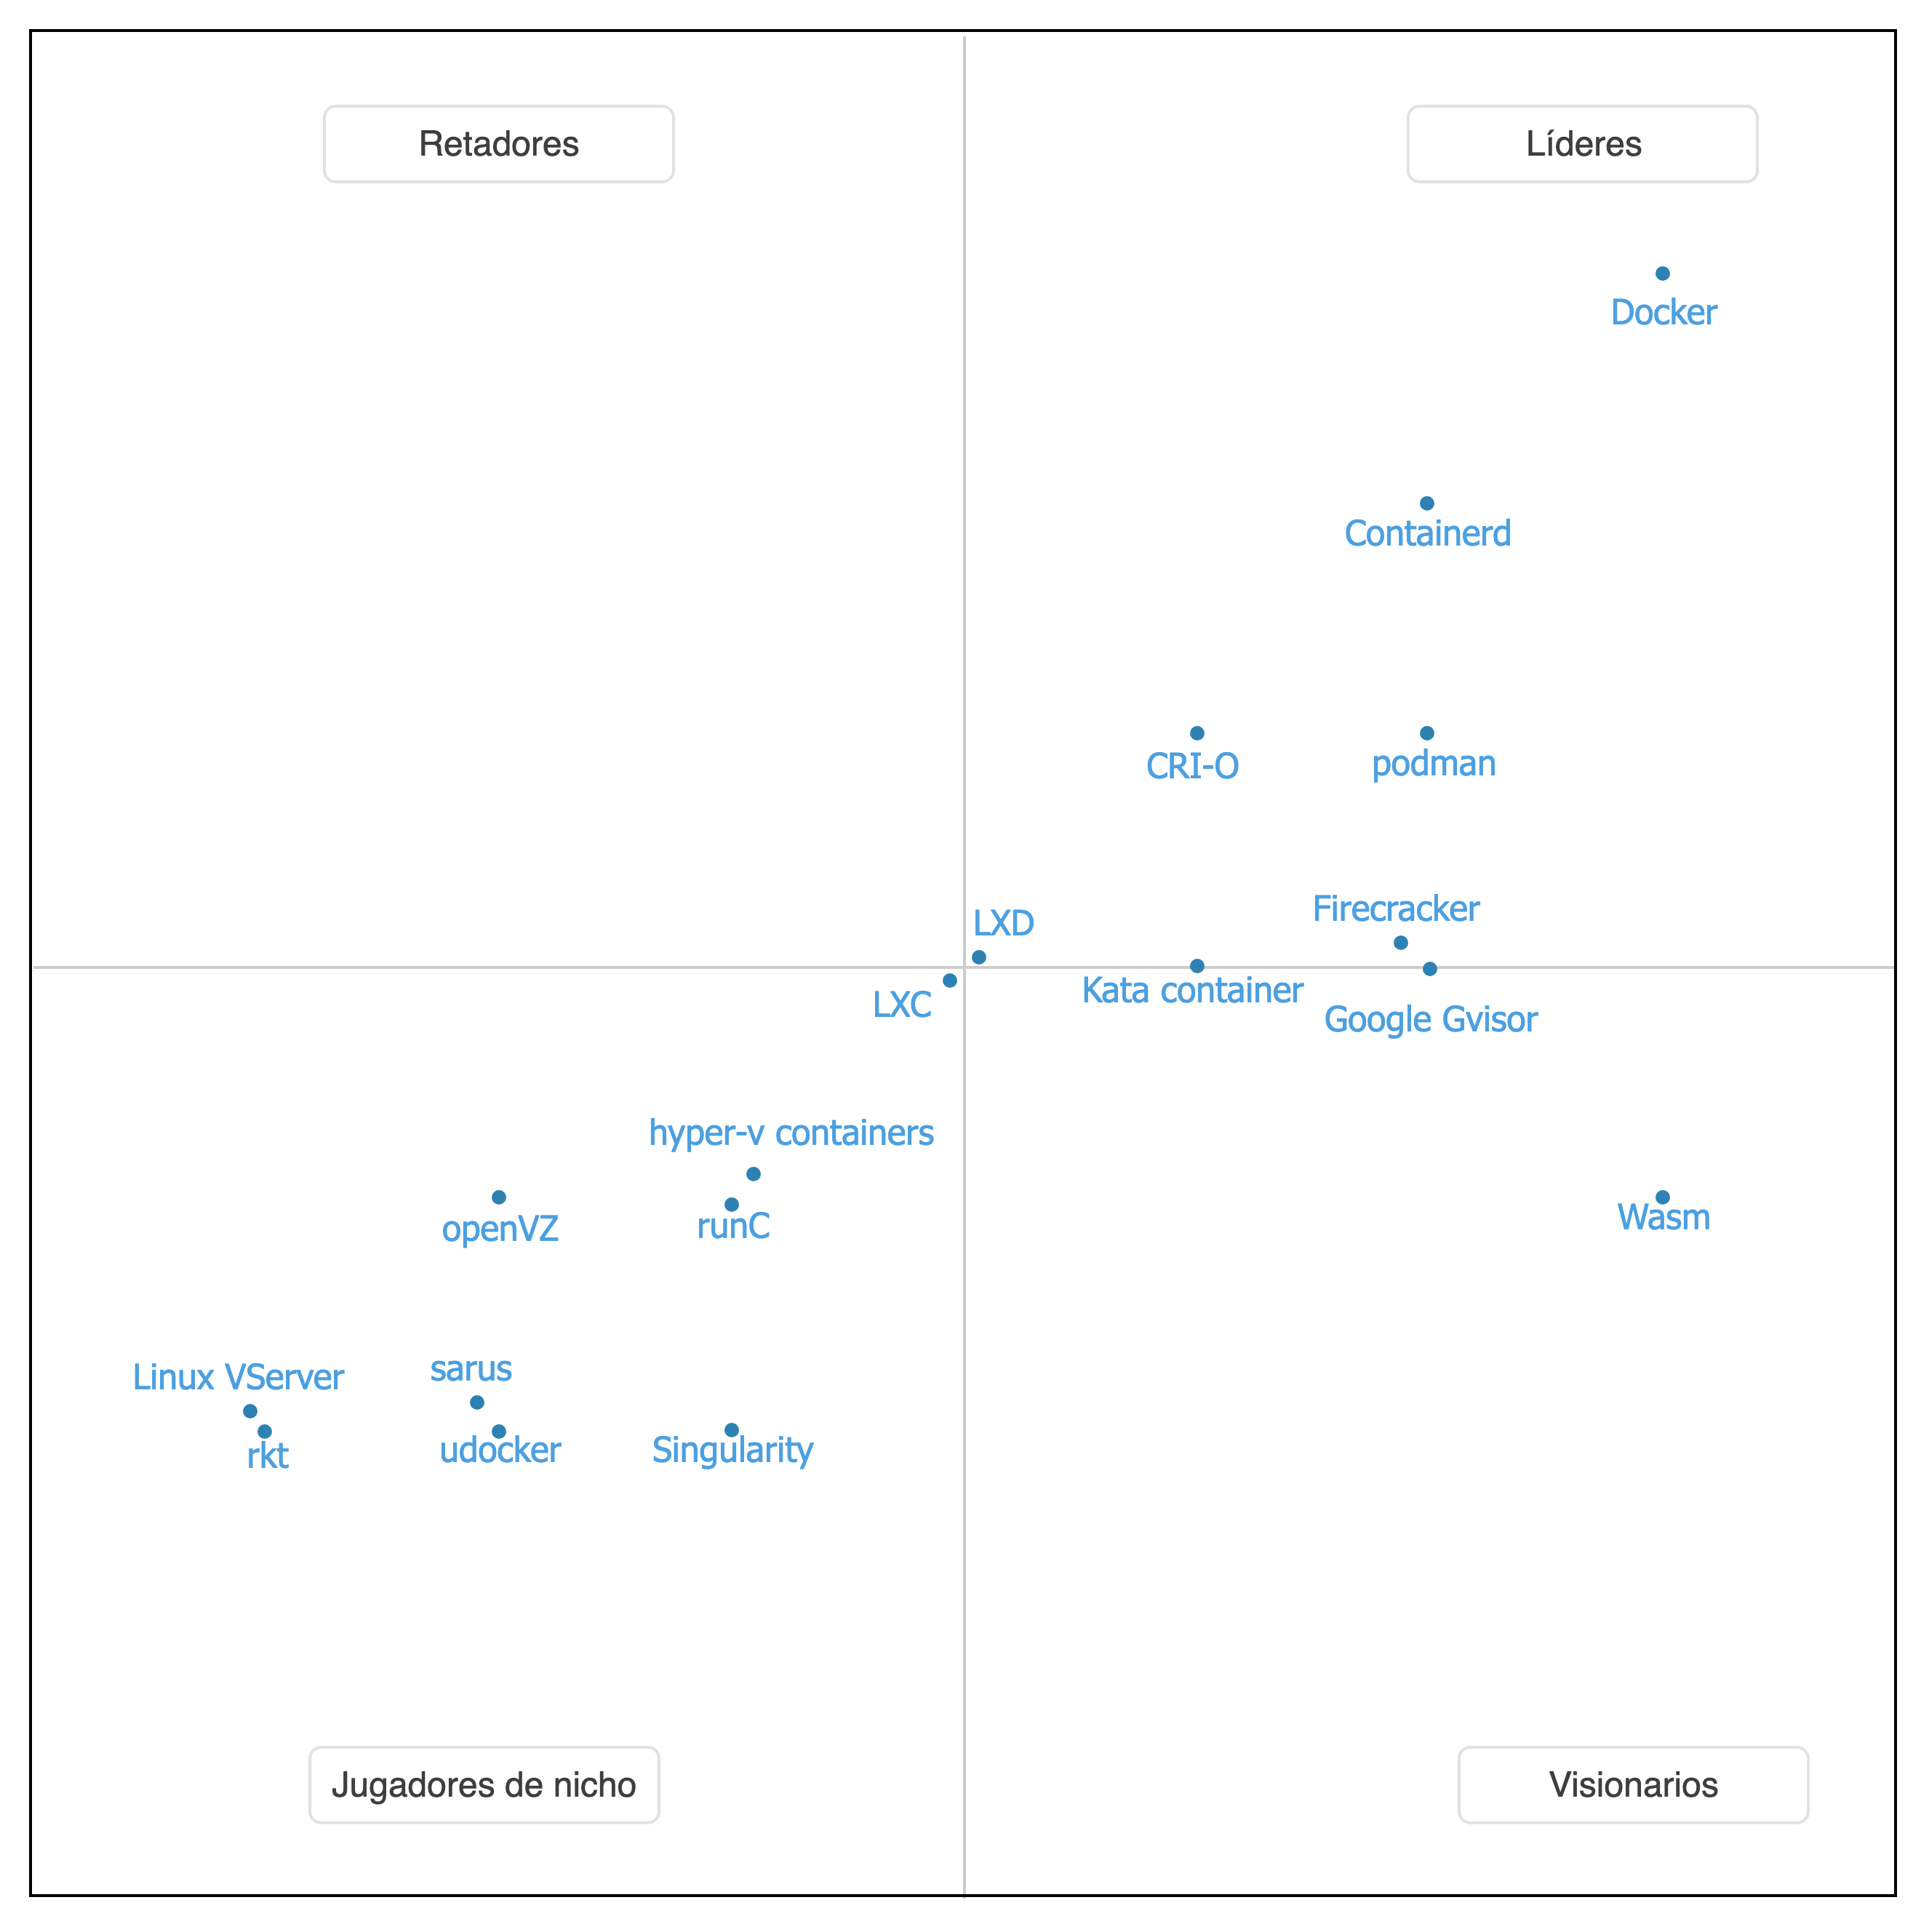
\includegraphics[width=\textwidth] {tablas-images/cp3/cuadrante-gartner.png}
    \caption{Cuadrante de Gartner de cada VBC}\label{fig:tabla-cuadrante-gartner}
\end{figure}

En la tabla~\ref{tab:entornos-ejecucion-vbc} se puede ver los sistemas operativos en los que se ejecutan estas tecnologias, se puede ver que la mayoria de estas estan diseñadas para sistemas linux, seguido de sistemas windows y por ultimo sistemas macOS, en cuyo caso las 2 unicas tecnologias que soportan este SO son ~\textit{Docker} y ~\textit{Podman}.
\begin{table}[H]
\centering
\scriptsize
\setlength{\tabcolsep}{3pt}
\renewcommand{\arraystretch}{1.1}
\begin{tabularx}{\textwidth}{|p{0.2\textwidth}|X|}
\hline
\textbf{Tecnología} & \textbf{Ambiente de Ejecución} \\
\hline
Docker & Sistemas Linux, Windows y macOS. Entornos de desarrollo, pruebas y producción, incluyendo la nube pública (\AWS, Google Cloud, Azure). \\
\hline
Podman & Sistemas Linux y macOS, con soporte experimental en Windows. Usado en entornos de desarrollo y producción sin necesidad de un daemon. \\
\hline
Udocker & Sistemas Linux, en entornos de computación de alto rendimiento (\HPC) y servidores compartidos, permitiendo ejecutar contenedores sin privilegios de root. \\
\hline
Wasm (WebAssembly) & Navegadores web (Chrome, Firefox, Safari, Edge). Ejecución en aplicaciones web y entornos de alto rendimiento sin dependencia del sistema operativo subyacente. \\
\hline
LXC & Sistemas Linux. Utilizado para crear contenedores ligeros que actúan como máquinas virtuales, con aplicaciones aisladas en servidores y plataformas de nube privada. \\
\hline
Containerd & Sistemas Linux y Windows. Usado en plataformas de orquestación como Kubernetes, y en infraestructuras de contenedores a gran escala. \\
\hline
LXD & Sistemas Linux. Virtualización ligera de contenedores como máquinas virtuales completas, ideal para servidores y plataformas de virtualización en la nube privada. \\
\hline
Rkt & Sistemas Linux. Anteriormente usado en entornos de orquestación de contenedores y en infraestructuras de nube privada. (Descontinuado actualmente). \\
\hline
Singularity & Sistemas Linux, especialmente en entornos de computación científica y \HPC\ . Portabilidad de aplicaciones científicas sin necesidad de privilegios de root. \\
\hline
runC & Sistemas Linux. Runtime ligero de contenedores compatible con los estándares de la Open Container Initiative (\OCI), utilizado por plataformas como Docker y Kubernetes. \\
\hline
CRI-O & Sistemas Linux. Integrado con Kubernetes para la gestión eficiente de contenedores en plataformas de orquestación en la nube y servidores locales. \\
\hline
Hyper-V containers & Sistemas Windows (Windows Server y Windows 10 con Hyper-V habilitado). Usado para contenedores con aislamiento mediante micro-VMs, ideal para entornos híbridos. \\
\hline
OpenVZ & Sistemas Linux. Virtualización a nivel de contenedor en proveedores de hosting para ofrecer entornos aislados y eficientes. \\
\hline
Linux VServer & Sistemas Linux. Contenedores que funcionan como servidores virtuales, usados en entornos de hosting y administración de servidores de alta disponibilidad. \\
\hline
Google gVisor & Plataformas de nube, especialmente Google Cloud. Capa adicional de seguridad para contenedores en entornos multitenant. \\
\hline
Kata Containers & Sistemas Linux. Virtualización ligera con aislamiento similar a máquinas virtuales, utilizado en plataformas de contenedores en la nube y servidores donde se requiere seguridad. \\
\hline
Firecracker & Plataformas de computación en la nube, como \AWS\ . Optimizado para micro-VMs ultra ligeras y de alto rendimiento en entornos serverless. \\
\hline
Sarus & Sistemas Linux. Entornos de computación de alto rendimiento (\HPC) y clústeres de supercomputación, proporcionando portabilidad y eficiencia sin privilegios de root. \\
\hline
\end{tabularx}
\caption{Entornos de ejecución de cada VBC}
\label{tab:entornos-ejecucion-vbc}
\end{table}

En el cuadro~\ref{tab:matriz-dofa} se define una matriz DOFA, especificando las debilidades, oportunidades, fortalezas y amenazas de las tecnologías VBC. Esto permite tener varios aspectos en cuenta a la hora de seleccionar una tecnología o realizar una implementación.
\begin{table}[H]
\centering
\scriptsize
\setlength{\tabcolsep}{4pt}
\renewcommand{\arraystretch}{1.2}
\begin{tabularx}{\textwidth}{|X|X|}
\hline
\multicolumn{1}{|c|}{\textbf{Fortalezas}} & \multicolumn{1}{c|}{\textbf{Oportunidades}} \\
\hline
\begin{minipage}[t]{\dimexpr\linewidth-8mm} % Reduced width for padding
\vspace{2pt}
\begin{itemize}
    \setlength\itemsep{0pt}
    \setlength\parskip{0pt}
    \setlength\parsep{0pt}
    \item \hspace{5mm} Herramientas como Kubernetes y Docker se actualizan constantemente, agregando nuevas funcionalidades y mejoras.
    \item \hspace{5mm} La \VBC\ es ampliamente utilizada en plataformas en la nube como AWS, Azure y Google Cloud.
    \item \hspace{5mm} Numerosos foros, grupos y organizaciones están dedicados a mejorar y desarrollar soluciones de contenerización.
    \item \hspace{5mm} Los contenedores pueden ejecutarse en múltiples entornos (local, nube, híbrido).
    \item \hspace{5mm} Permiten una mejor utilización de recursos en comparación con las máquinas virtuales tradicionales.
\end{itemize}
\vspace{2pt}
\end{minipage}
\hspace{4mm} % Right padding
&
\begin{minipage}[t]{\dimexpr\linewidth-8mm} % Reduced width for padding
\vspace{2pt}
\begin{itemize}
    \setlength\itemsep{0pt}
    \setlength\parskip{0pt}
    \setlength\parsep{0pt}
    \item \hspace{5mm} Los contenedores son ligeros y comparten el kernel del sistema operativo, reduciendo el consumo de recursos.
    \item \hspace{5mm} Una aplicación en contenedor puede ejecutarse en cualquier entorno compatible sin modificaciones.
    \item \hspace{5mm} Permiten implementar y gestionar aplicaciones de manera escalable y eficiente.
    \item \hspace{5mm} Los contenedores permiten que las aplicaciones se ejecuten de manera independiente, evitando conflictos entre ellas.
    \item \hspace{5mm} Herramientas como Docker Compose y Kubernetes facilitan la gestión automatizada de contenedores.
\end{itemize}
\vspace{2pt}
\end{minipage}
\hspace{4mm} % Right padding
\\
\hline
\multicolumn{1}{|c|}{\textbf{Debilidades}} & \multicolumn{1}{c|}{\textbf{Amenazas}} \\
\hline
\begin{minipage}[t]{\dimexpr\linewidth-8mm} % Reduced width for padding
\vspace{2pt}
\begin{itemize}
    \setlength\itemsep{0pt}
    \setlength\parskip{0pt}
    \setlength\parsep{0pt}
    \item \hspace{5mm} Los contenedores comparten el mismo núcleo del sistema operativo host, lo que podría permitir que una vulnerabilidad afecte a todos los contenedores.
    \item \hspace{5mm} A medida que crece la infraestructura, gestionar múltiples contenedores y sus redes se vuelve complejo.
    \item \hspace{5mm} A diferencia de las máquinas virtuales tradicionales, los contenedores son efímeros por diseño, lo que complica el manejo de datos persistentes.
    \item \hspace{5mm} No todos los sistemas y aplicaciones son compatibles de manera nativa con contenedores, lo que requiere configuraciones específicas.
    \item \hspace{5mm} La seguridad y rendimiento de los contenedores están directamente relacionados con el sistema operativo subyacente.
\end{itemize}
\vspace{2pt}
\end{minipage}
\hspace{4mm} % Right padding
&
\begin{minipage}[t]{\dimexpr\linewidth-8mm} % Reduced width for padding
\vspace{2pt}
\begin{itemize}
    \setlength\itemsep{0pt}
    \setlength\parskip{0pt}
    \setlength\parsep{0pt}
    \item \hspace{5mm} Si no se aplican buenas prácticas, los contenedores pueden ser vulnerables a ataques.
    \item \hspace{5mm} El uso de soluciones propietarias como \AWS\ o Azure puede generar dependencia tecnológica.
    \item \hspace{5mm} Las tecnologías de contenerización evolucionan rápidamente, lo que puede dejar obsoletas algunas soluciones.
    \item \hspace{5mm} Un mal diseño puede llevar a un consumo ineficiente de recursos.
    \item \hspace{5mm} Aunque existen buenas prácticas, no hay una regulación estándar única para la gestión de contenedores.
\end{itemize}
\vspace{2pt}
\end{minipage}
\hspace{4mm} % Right padding
\\
\hline
\end{tabularx}
\caption{Tabla de matriz DOFA para el cuadrante gartner}\label{tab:matriz-dofa}
\end{table}
\begin{table}[H]
\centering
\scriptsize
\setlength{\tabcolsep}{3pt}
\renewcommand{\arraystretch}{1.1}
\begin{tabular}{|>{\raggedright\arraybackslash}p{4cm}|>{\centering\arraybackslash}p{2.5cm}|}
\hline
\centering\textbf{Tecnología} & \textbf{Documentación} \\
\hline
Docker & \href{https://docs.docker.com/}{link} \\
\hline
Podman & \href{https://podman.io/docs}{link} \\
\hline
Udocker & \href{https://github.com/indigo-dc/udocker}{link} \\
\hline
Wasm & \href{https://webassembly.org/docs/faq/}{link} \\
\hline
LXC & \href{https://linuxcontainers.org/incus/docs/main/}{link} \\
\hline
Containerd & \href{https://containerd.io/docs/}{link} \\
\hline
LXD & \href{https://linuxcontainers.org/incus/docs/main/}{link} \\
\hline
Rkt & \href{https://github.com/rkt/rkt}{link} \\
\hline
Singularity & \href{https://docs.sylabs.io/guides/4.3/user-guide/}{link} \\
\hline
runC & \href{https://github.com/opencontainers/runc}{link} \\
\hline
CRI-O & \href{https://github.com/cri-o/cri-o}{link} \\
\hline
Hyper-V containers & \href{https://docs.microsoft.com/en-us/virtualization/windowscontainers/}{link} \\
\hline
OpenVZ & \href{https://openvz.org/}{link} \\
\hline
Linux VServer & \href{http://linux-vserver.org/Documentation}{link} \\
\hline
Google gVisor & \href{https://gvisor.dev/docs/}{link} \\
\hline
Kata Containers & \href{https://katacontainers.io/docs/}{link} \\
\hline
Firecracker & \href{https://firecracker-microvm.github.io/}{link} \\
\hline
Sarus & \href{https://github.com/eth-cscs/sarus}{link} \\
\hline
\end{tabular}
\caption{Enlaces a la documentación de tecnologías de contenerización}
\label{tab:documentacion-tecnologias}
\end{table}
%\ChapterImageStar[cap:benchmarking]{Benchmarking}{./images/fondo.png}\label{cap:benchmarking}

\mbox{}\\
\section{Definición de las pruebas}

Para evaluar el rendimiento de distintas tecnologías de contenerización —específicamente Docker, Podman, LXC, LXD y Containerd— se diseñó un conjunto de pruebas orientadas a medir aspectos clave del desempeño en entornos controlados. Las pruebas incluyeron el consumo de CPU y memoria RAM, el tiempo de arranque de los contenedores, el \textit{throughput} de red y la latencia de acceso a disco. 

Para garantizar la repetibilidad y objetividad de los resultados, se desarrollaron scripts en \textit{Bash} que automatizan la ejecución de cada métrica en condiciones homogéneas. Estas pruebas permiten comparar las tecnologías evaluadas bajo criterios cuantificables y facilitar un análisis técnico de sus capacidades en escenarios reales de uso.

\section{Construcción de las pruebas}

La construcción de las pruebas se llevó a cabo mediante el desarrollo de scripts automatizados en \textit{Bash}, diseñados para ejecutarse de forma uniforme sobre cada tecnología de contenerización evaluada. Cada script fue responsable de iniciar contenedores, ejecutar cargas de trabajo específicas y recolectar métricas de rendimiento relevantes.

Para medir el consumo de CPU y memoria RAM, se utilizó \texttt{pidstat}, una utilidad que permite la medición del consumo de recursos. El tiempo de arranque se determinó midiendo el intervalo entre la orden de inicio del contenedor y el momento en que estuvo completamente operativo. 

Para evaluar el \textit{throughput} de red se emplearon herramientas como \texttt{iperf}, mientras que la latencia de disco fue medida utilizando \texttt{fio}. Todas las pruebas fueron ejecutadas múltiples veces para reducir el impacto de variaciones puntuales y asegurar la confiabilidad de los resultados. Los scripts fueron programados para ejecutarse 10 veces; al final se extrae un promedio y este constituye el puntaje final de la tecnología de contenerización en cuestión.

En el repositorio \underline{\href{https://github.com/Anubis-1001/benchmark-tecnologias-de-contenerizacion} {\texttt{ GitHub benchmarking}}} se pueden encontrar los scripts resultantes de este proceso.

\section{Resultados de las pruebas}

Los resultados obtenidos a partir de las pruebas evidencian diferencias significativas en el rendimiento entre las tecnologías de contenerización evaluadas. Estos se pueden consultar en el archivo de Excel \underline{\href{https://docs.google.com/spreadsheets/d/1Ce37Sm3Swyfa88Ur1yQbLarq_D86obUIAGGJocgQbUE/edit?usp=sharing} {\texttt{benchmarking\_tecnologias}}}.

En términos de consumo de CPU, Docker y Containerd presentan las mejores métricas; en consumo de memoria RAM, LXC y LXD mostraron un mejor uso de los recursos. En cuanto al tiempo de arranque, Containerd destacó por su velocidad, seguido de cerca por Docker, mientras que LXC presentó un arranque considerablemente más lento en comparación con las demás tecnologías.

Para el \textit{throughput} de red, todas las tecnologías mostraron un desempeño comparable, siendo LXC el más destacado; no obstante, Podman quedó muy por debajo en esta métrica. Finalmente, en la medición de latencia de disco, LXD y Containerd obtuvieron los mejores resultados, lo que sugiere una gestión de E/S más directa y liviana.

Estos resultados permiten establecer un panorama claro de fortalezas y debilidades de cada solución, según el tipo de carga o entorno de ejecución esperado.

\section{Métricas de rendimiento}

De la ejecución de las pruebas se obtuvieron las siguientes métricas de rendimiento:

\begin{figure}[H]
    \centering
    \includegraphics[scale=0.5] {tablas-images/cp4/cpu.png}
    \caption{Métricas de uso de CPU}\label{fig:tabla-metricas-cpu}
\end{figure}
\begin{figure}[H]
    \centering
    \includegraphics[width=\textwidth] {tablas-images/cp4/ram.png}
    \caption{Métricas de uso de RAM}\label{fig:tabla-metricas-ram}
\end{figure}
\begin{figure}[H]
    \centering
    \includegraphics[width=\textwidth] {tablas-images/cp4/io.png}
    \caption{Métricas de entrada/salida}\label{fig:tabla-metricas-io}
\end{figure}
\begin{figure}[H]
    \centering
    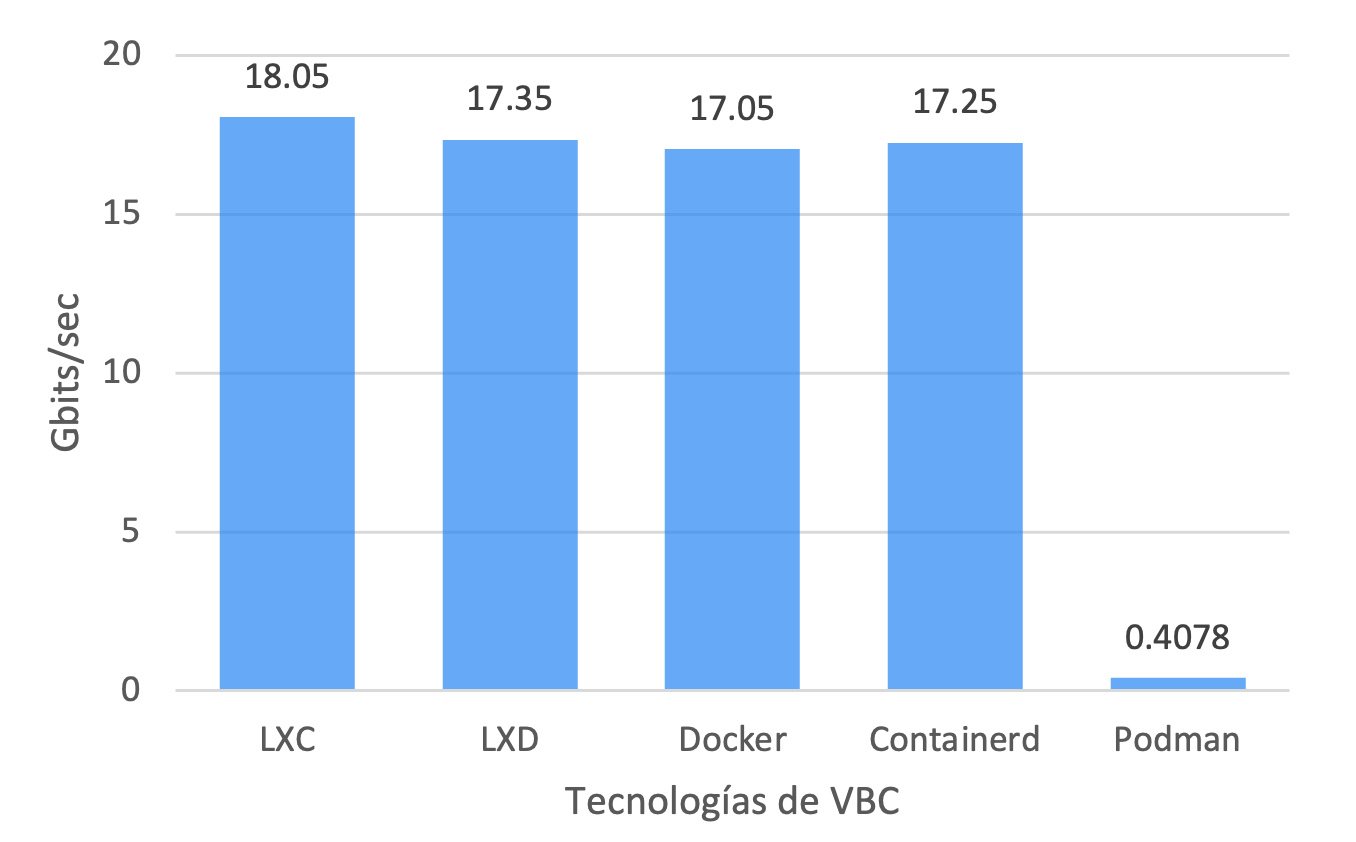
\includegraphics[width=\textwidth] {tablas-images/cp4/THROUGHTPUT.png}
    \caption{Métricas de throughput}\label{fig:tabla-metricas-throughput}
\end{figure}

\section{Análisis de los resultados}

Los resultados obtenidos a partir de las pruebas permiten identificar comportamientos diferenciados entre las tecnologías de contenerización evaluadas. \textbf{Containerd} se posiciona como una de las soluciones más equilibradas, con excelente tiempo de arranque, bajo uso de CPU y buena latencia de disco, lo que lo hace ideal para entornos donde la eficiencia es prioritaria.

\textbf{LXC} mostró consistentemente el menor consumo de recursos y alto rendimiento en red, lo que lo convierte en una opción sólida para sistemas embebidos o despliegues que requieren un uso mínimo de \textit{overhead}. 

Por otro lado, \textbf{Docker} ofreció un rendimiento aceptable, pero con mayores niveles de consumo de CPU y latencia de disco, compensados por su madurez y ecosistema. 

\textbf{LXD}, al estar basado en LXC, heredó parte de sus beneficios, especialmente en uso de red, aunque con un ligero incremento en el tiempo de arranque. 

En contraste, \textbf{Podman}, si bien eficiente en uso de CPU y memoria, presentó resultados considerablemente bajos en el \textit{throughput} de red y alta latencia de disco, lo cual podría limitar su aplicación en cargas sensibles a E/S o comunicación intensiva.

\vspace{0.5em}

\noindent En resumen, la elección de la tecnología de contenerización debe considerar el caso de uso específico: \textbf{Containerd} y \textbf{LXC} sobresalen en eficiencia general; \textbf{Docker} y \textbf{LXD} ofrecen robustez y facilidad de integración; mientras que \textbf{Podman} puede ser más adecuado para entornos que prioricen la seguridad y compatibilidad con el modelo sin \textit{daemon}, siempre que el rendimiento de red o disco no sea crítico.

%\ChapterImageStar[cap:dar]{Análisis de Decisiones y Resolución}{./images/fondo.png}\label{cap:dar}
\mbox{}\\
\section{Metodología de evaluación}

La metodología de evaluación que se aplicó para la elección de la tecnología de Virtualización Basada en Contenedores (VBC) fue DAR (Decision, analysis and resolution) de CMMI \citep{CMMIInstitute2010}. Esta metodología permitió evaluar las necesidades del grupo GRID a través de un proceso estructurado que consideró múltiples alternativas, criterios de evaluación bien definidos y un análisis comparativo. En este caso, se identificaron y analizaron diversas tecnologías VBC —como Docker, Podman, LXC o Kata Containers— aplicando criterios como el tipo de licencia, la compatibilidad con herramientas de orquestación, el rendimiento entre otros. Mediante el uso de matrices DOFA, se logró visualizar las fortalezas y debilidades de cada opción, facilitando una selección alineada con los objetivos estratégicos del sistema. Así, el uso de DAR no solo aportó transparencia al proceso, sino también trazabilidad y justificación técnica frente a una decisión para la arquitectura de infraestructura basada en contenedores.

El proceso de evaluación quedó registrado en un vídeo explicativo disponible en \href{https://youtu.be/xOmuQs2RX2c}{link}.

\section{Resultados de la evaluación}

\begin{table}[H]
    \centering
    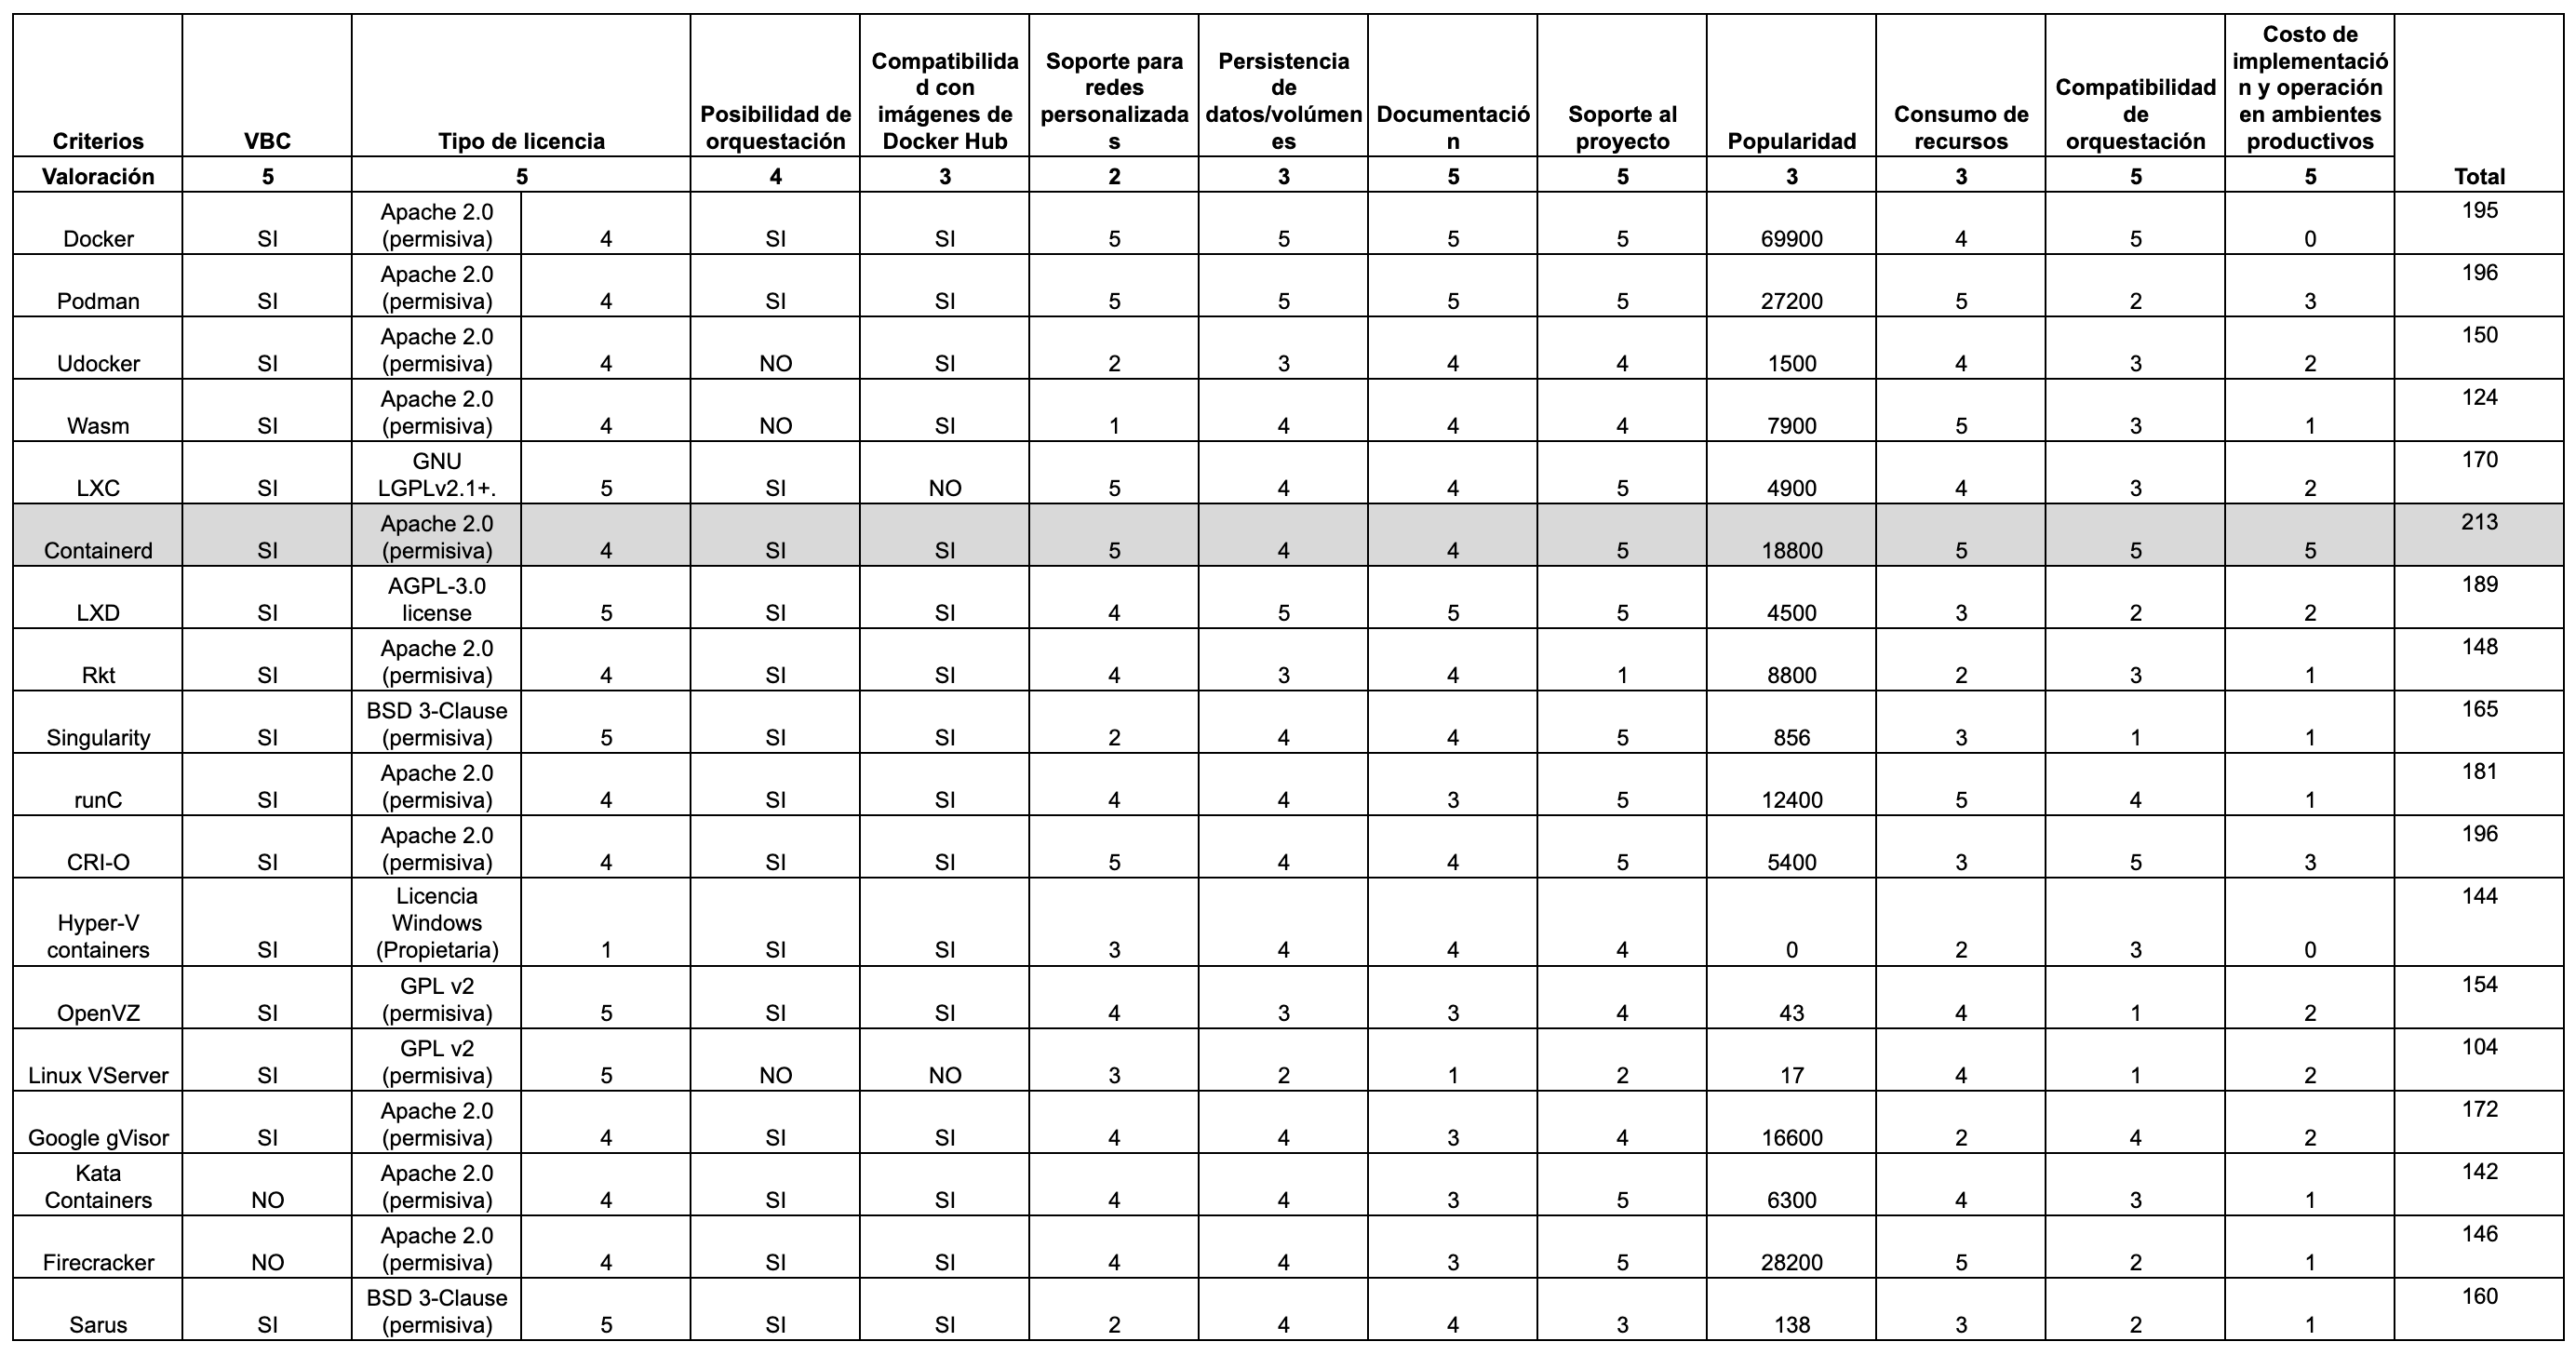
\includegraphics[width=\textwidth] {tablas-images/cp5/DAR.png}
    \caption{Análisis de Decisiones y Resolución (DAR) aplicado a la selección de VBC}\label{tab:tabla-dar}
\end{table}

\section{Criterios de evaluación}

\subsection{VBC (¿Es una tecnología basada en contenedores?)}
Este criterio define si la tecnología analizada entra dentro de la categoría de virtualización basada en contenedores, lo cual es el punto de partida para que pueda ser considerada en el análisis. Se evalúa como Sí (SI) o No (NO).

\subsection{Tipo de licencia}
Se analiza el tipo de licencia bajo la cual se distribuye la tecnología, ya que esto afecta su adopción en proyectos académicos o comerciales. Las licencias permisivas (como Apache 2.0 o BSD) permiten mayor libertad de uso y modificación, mientras que licencias restrictivas (como AGPL o licencias propietarias) imponen ciertas limitaciones legales o técnicas.

\subsection{Posibilidad de orquestación}
Se refiere a la capacidad de la tecnología para integrarse con herramientas de orquestación como Kubernetes, Docker Swarm o Nomad, lo cual es clave para la gestión automatizada de contenedores a gran escala. Una mayor puntuación indica mejor compatibilidad y soporte para estas herramientas.

\subsection{Compatibilidad con imágenes de Docker Hub}
Evalúa si la tecnología puede ejecutar imágenes obtenidas directamente desde Docker Hub, el repositorio más utilizado para contenedores. Esto facilita la reutilización de contenedores existentes y la integración con flujos de trabajo ya establecidos.

\subsection{Soporte para redes personalizadas}
Determina si la tecnología permite la creación y gestión de redes personalizadas entre contenedores. Este aspecto es fundamental en arquitecturas distribuidas, donde la comunicación entre servicios debe configurarse de forma segura.

\subsection{Persistencia de datos / volúmenes}
Analiza si la solución permite la persistencia de datos, es decir, que los datos generados dentro de un contenedor puedan mantenerse incluso después de reiniciarlo o eliminarlo. Esto se logra mediante el uso de volúmenes o sistemas de almacenamiento externos.

\subsection{Documentación}
Se valora la calidad, profundidad y accesibilidad de la documentación oficial. Una buena documentación facilita el aprendizaje, la resolución de problemas y la implementación efectiva de la tecnología.

\subsection{Soporte al proyecto}
Considera el respaldo que tiene la tecnología por parte de la comunidad, empresas o fundaciones (como CNCF o Red Hat). Esto incluye mantenimiento activo, actualizaciones regulares, y foros o canales de ayuda disponibles.

\subsection{Popularidad}
Este criterio mide la adopción y visibilidad de la tecnología, lo cual puede reflejar su madurez, confianza del mercado y disponibilidad de talento capacitado. Se puede estimar por métricas como el número de estrellas en GitHub.

\subsection{Consumo de recursos}
Evalúa el nivel de consumo de recursos respecto al uso de CPU, memoria y almacenamiento. Se valora según lo que mencionan las organizaciones en este aspecto.

\subsection{Compatibilidad de orquestación}
Difiere levemente del punto 4.3, ya que aquí se mide qué tan bien se integra con los orquestadores, considerando estabilidad, plugins nativos y experiencia de uso. Un puntaje alto indica integración fluida y confiable.

\subsection{Costo de implementación y operación en ambientes productivos}
Este criterio analiza los costos asociados a poner en marcha la tecnología en un entorno real. Incluye licencias, infraestructura, tiempo de configuración y mantenimiento. Una puntuación alta significa bajo costo o costo nulo, lo cual es ideal para instituciones académicas o proyectos con presupuesto limitado.

\section{Tecnología VBC ganadora}

Del análisis comparativo realizado, Containerd se posiciona como la tecnología de virtualización basada en contenedores con mejor desempeño general. Destaca por su alta compatibilidad con Docker Hub, soporte para redes y volúmenes, excelente integración con orquestadores como Kubernetes, y una licencia permisiva que facilita su adopción. Además, cuenta con una sólida documentación y un respaldo activo de la comunidad. Estas características hacen de Containerd la opción adecuada para ser implementada en ambientes productivos del grupo de investigación GRID, combinando los diferentes criterios definidos desde el grupo de investigación.

\section{Análisis DAR del motor de Kubernetes}

\begin{table}[H]
    \centering
    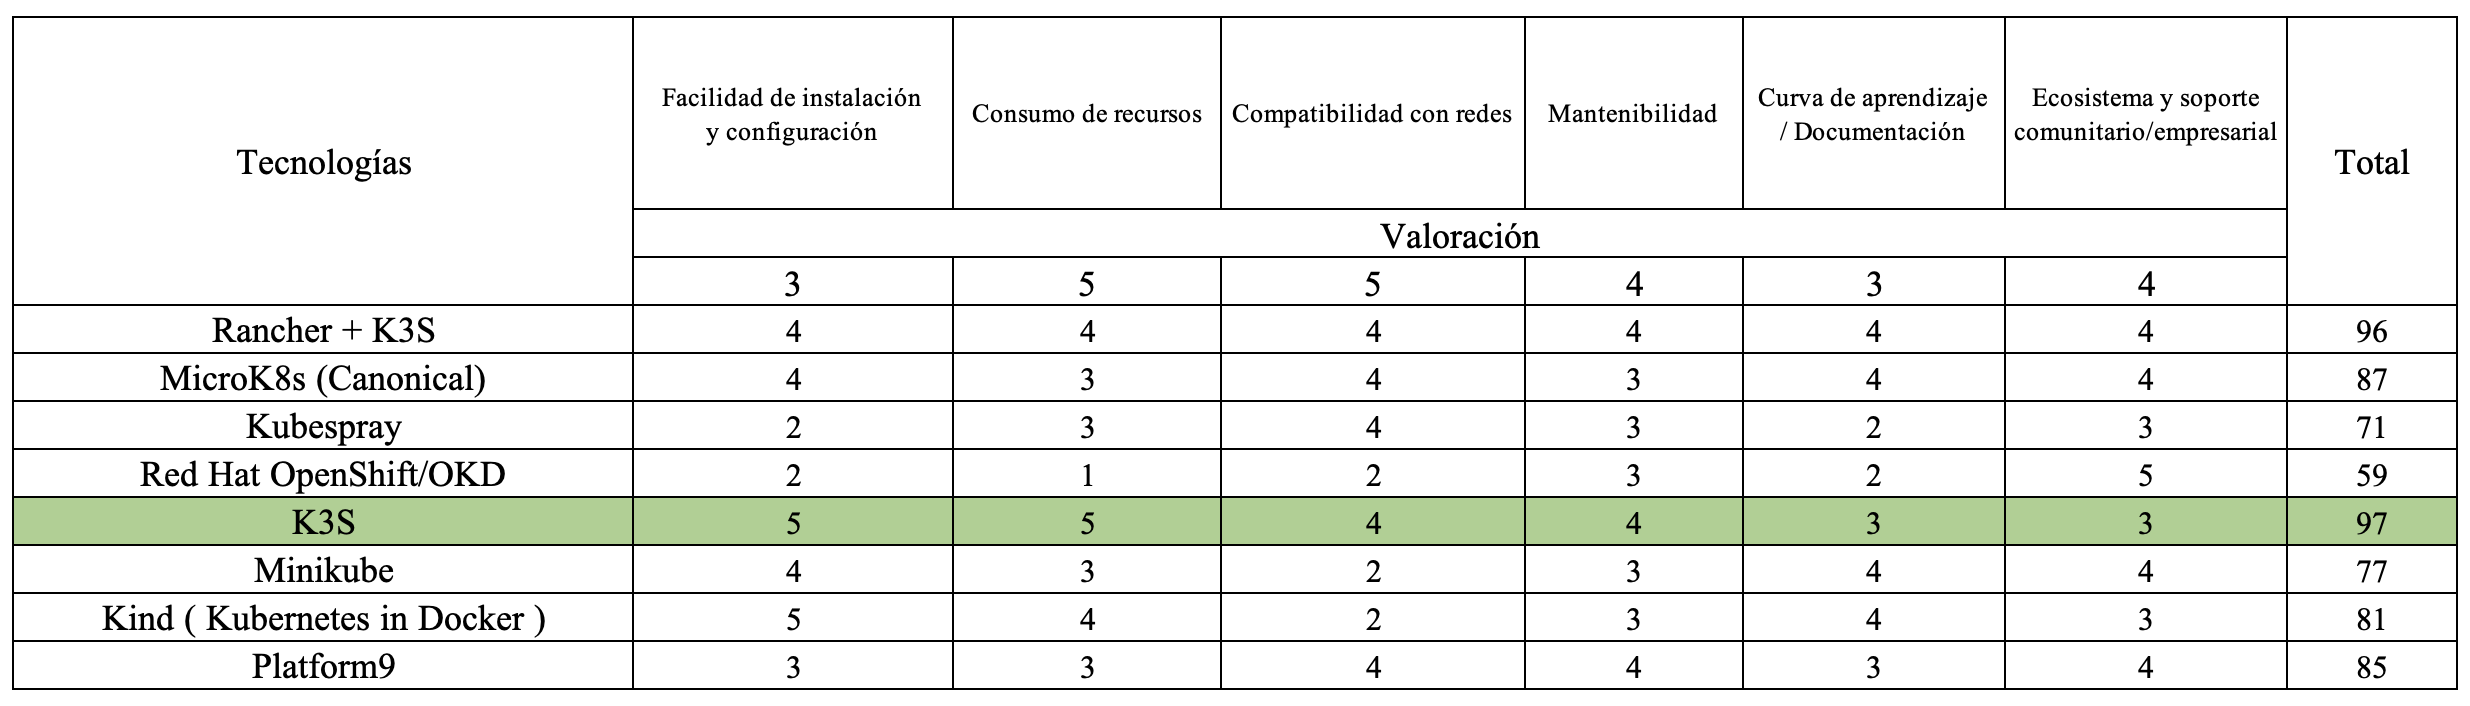
\includegraphics[width=\textwidth] {tablas-images/cp5/dar-k8s.png}
    \caption{Análisis de Decisiones y Resolución aplicado a la selección del motor de Kubernetes}\label{tab:tabla-dar}
\end{table}
%\ChapterImageStar[cap:disenio]{Diseño de la solución}{./images/fondo.png}\label{cap:disenio}
\mbox{}\\

El presente capítulo tiene como objetivo fundamental traducir la decisión estratégica —la implementación de los Universos Grid y Parallel— en un diseño técnico y estratégico concreto y ejecutable. Aquí se especifica la arquitectura de la solución, detallando los componentes de HTCondor que serán configurados o modificados, los flujos de trabajo establecidos para cada universo y los criterios de interoperabilidad con el Universo Vanilla preexistente. Este diseño busca establecer las bases técnicas y metodológicas para la fase de implementación, propendiendo por la robustez, escalabilidad e integridad de la infraestructura de computación distribuida resultante. Además, busca ayudar al Grupo \GRID con el cumplimiento de sus objetivos estratégicos y el cierre de la brecha identificada en la caracterización.

\section{Definición de estrategia}
La definición de la estrategia de diseño se fundamenta en una filosofía de desarrollo guiado por pruebas (\TDD), que es una disciplina de diseño y programación donde cada línea de código está escrita en respuesta a una prueba que el programador escribe justo antes de escribir el código \parencite{4163024}. Antes de especificar los componentes arquitectónicos, se establece un conjunto de casos de prueba estructurados que definen de manera formal y verificable el comportamiento esperado de los Universos \textit{Grid} y \textit{Parallel}. Estos casos, que funcionan como criterios de aceptación guiarán de manera iterativa el diseño de la solución, asegurando que cada decisión de implementación esté directamente alineada con la validación funcional del sistema.

Por último, se considera necesario establecer un nombre para el sistema. Esto con el fin de dar mayor claridad al lector y hacer más visibles los momentos en los que se habla del sistema resultado de este proyecto. Se opta por el "Grid App" haciendo referencia al Grupo \GRID, que es el sujeto nuclear de este proyecto; al Universo Grid, que es uno de los Universos que se decidió implementar para este proyecto de aplicación después de la toma de decisiones estructurada mediante el análisis \DAR y el modelo computacional Grid que es básicamente una infraestructura que provee gran capacidad computacional a un sistema distribuido haciendo uso de recursos geográficamente distribuidos \parencite{8974490}.

\section{Casos de prueba}

\subsection{Definición de requisitos}
\noindent
Para iniciar con la definición de casos de prueba, se establecen los requisitos que debe cumplir \textit{Grid App} que están fundamentados en el análisis preliminar hecho anteriormente, principalmente en la descripción de la oportunidad para el Grupo \GRID.

\subsubsection{Requisitos funcionales}
\noindent
Según \textcite{159342} un requisito funcional especifica una función que el sistema o que un componente del sistema es capaz de hacer. A continuación se definen los requisitos funcionales para \textit{Grid App}.
\begin{table}[H]
	\centering
	\sffamily\scriptsize
	\setlength{\tabcolsep}{4pt}
	\renewcommand{\arraystretch}{1.3}
	\caption{Requisitos funcionales para \textit{Grid App}}
	\label{table:requisitosFuncionales}
	\begin{tabular}{|p{0.1\textwidth}|p{0.2\textwidth}|p{0.7\textwidth}|}
		\toprule
		\textbf{ID}                              & \textbf{Título}                               & \textbf{Descripción} \\
		\midrule
		RF1 & Soporte para Universos adicionales & El sistema debe permitir la ejecución de trabajos en al menos dos Universos adicionales a Vanilla (Grid y Parallel) \\
		\midrule
		RF2 & Orquestación de múltiples clústeres & El sistema debe permitir enviar trabajos hacia diferentes clústeres (Parallel, Vanilla) a través del Universo Grid. \\
		\midrule
		RF3 & Selección de destino & El sistema debe permitir que el usuario especifique el clúster de destino. \\
		\midrule
		RF4 & Monitoreo de trabajos & El sistema debe permitir el monitoreo de los trabajos enviados a los clústeres, mostrando su estado al usuario. \\
		\midrule
		RF5 & Ejecución MPI en Parallel & Un clúster debe soportar ejecución de trabajos basados en MPI en múltiples nodos (≥ N nodos configurados). \\
		\midrule
		RF6 & Redirección Grid-Parallel & El Grid Manager debe aceptar trabajos enviados al Universo Grid y, si la naturaleza del trabajo es paralelo, redirigirlos correctamente al Universo Parallel. \\
        \midrule
		RF7 & Redirección Grid-Vanilla & El Grid Manager debe aceptar trabajos enviados al Universo Grid y, si la naturaleza del trabajo es distribuido, redirigirlos correctamente al Universo Vanilla. \\
        \midrule
		RF8 & Registro centralizado de errores & El Grid Manager debe centralizar \textit{logs} de fallos de ejecución provenientes de cada clúster. \\
		\bottomrule
	\end{tabular}
\end{table}

\subsubsection{Requisitos no-funcionales}
\noindent
Según \textcite{4384163} un requisito no-funcional es un atributo o una restricción de un sistema. A continuación se definen los requisitos no-funcionales para \textit{Grid App}.
\begin{table}[H]
	\centering
	\sffamily\scriptsize
	\setlength{\tabcolsep}{4pt}
	\renewcommand{\arraystretch}{1.3}
	\caption{Requisitos no-funcionales para \textit{Grid App}}
	\label{table:requisitosNoFuncionales}
	\begin{tabular}{|p{0.1\textwidth}|p{0.2\textwidth}|p{0.7\textwidth}|}
		\toprule
		\textbf{ID}                              & \textbf{Título}                               & \textbf{Descripción} \\
		\midrule
		RNF1 & Transparencia de uso & El usuario no debe preocuparse por las configuraciones internas de cada clúster; el Grid Manager abstrae el destino mediante una interfaz más amigable. \\
		\midrule
		RNF2 & Usabilidad & La configuración de los nuevos Universos debe estar documentada y ser accesible mediante manual de despliegue para los usuarios del Grupo GRID. \\
		\midrule
		RNF3 & Disponibilidad & En caso de que un clúster esté inactivo, el Grid Manager debe registrar el error y permitir redirección a otro clúster disponible si el Universo es compatible. \\
		\bottomrule
	\end{tabular}
\end{table}

\subsection{Pruebas}
\noindent
Para esta sección, se definen las pruebas y los pasos de cada prueba a ejecutar 

\section{Modelado del sistema en Archimate}
ArchiMate es un lenguaje de modelado estandarizado por~\textit{The Open Group} que permite representar de manera estructurada y clara las diferentes capas de una arquitectura empresarial: negocio, aplicación y tecnología. Su propósito es brindar una visión integrada que facilite la comunicación entre los distintos actores de un proyecto y que muestre cómo los procesos de negocio, los sistemas de información y la infraestructura tecnológica se relacionan entre sí.
En particular, ArchiMate se organiza en vistas que permiten enfocarse en aspectos específicos: la vista de negocio describe los procesos y actores implicados, la vista de aplicación se centra en los sistemas de software que apoyan esos procesos, y la vista de tecnología aborda la infraestructura que soporta todo el ecosistema. Gracias a este enfoque por capas, los diagramas ayudan a identificar dependencias, puntos de optimización y la coherencia general de la solución arquitectónica.

\subsection{Vista de negocio}
El diagrama~\ref{fig:vista-cooperacion-actores} representa a los distintos actores involucrados en el sistema, como estudiantes, administrativos, docentes y el propio grupo de investigación GRID. El diagrama muestra cómo se comunican entre sí y cómo intercambian información, destacando elementos como cursos, programas, relaciones contractuales y archivos. En esencia, este diagrama ilustra las interacciones humanas y organizacionales necesarias para el funcionamiento del sistema.

\begin{figure}[H]
    \centering
    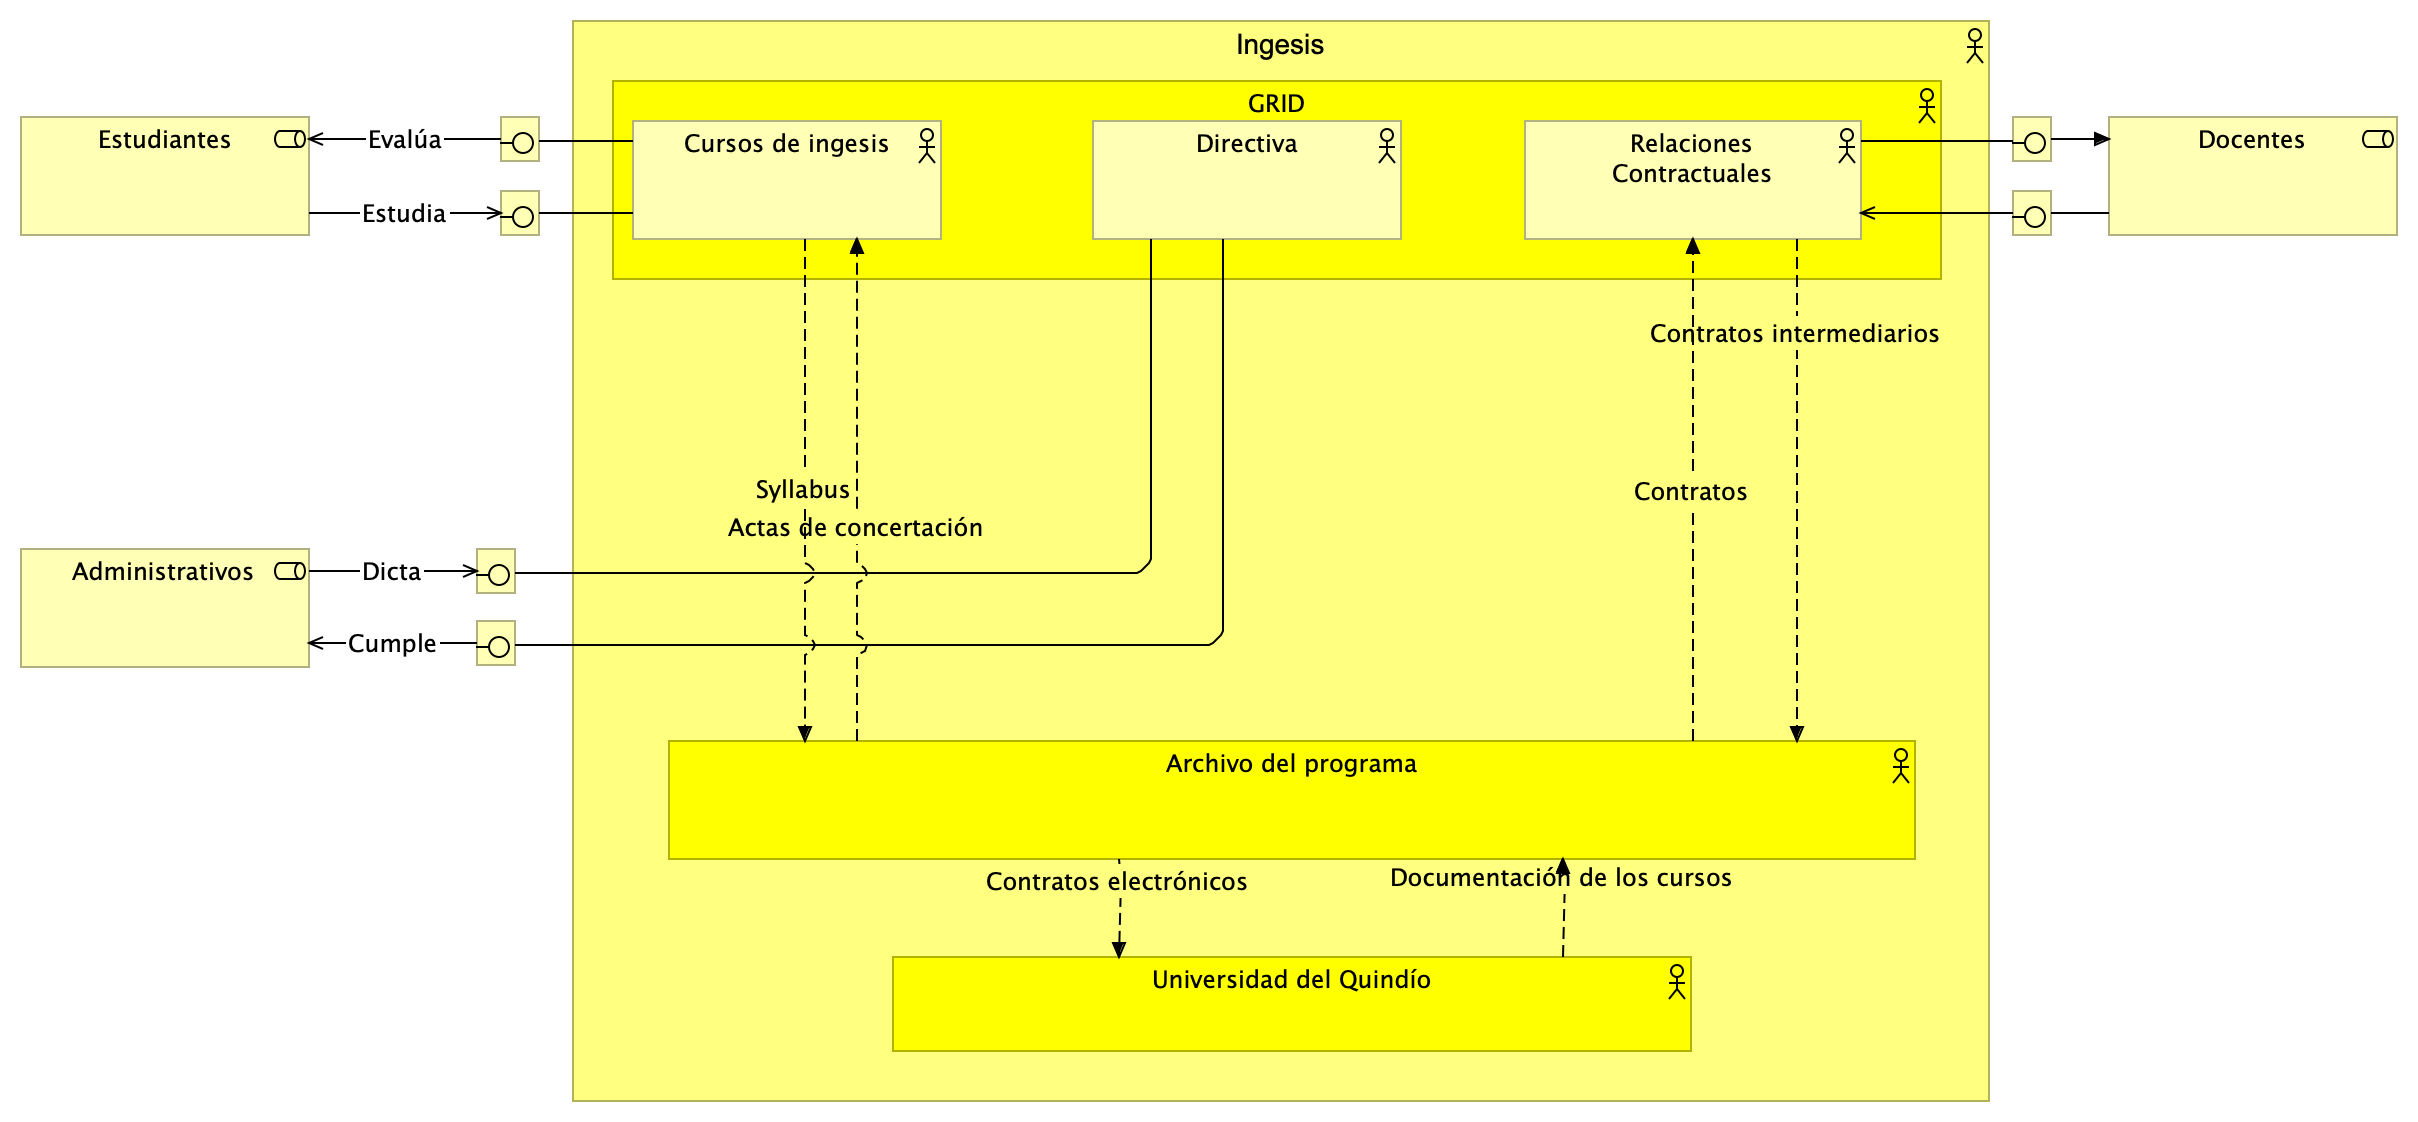
\includegraphics[width=\textwidth]{tablas-images/cp6/Actor-Cooperation-view.png}
    \caption{Vista de Cooperación de Actores}\label{fig:vista-cooperacion-actores}
\end{figure}

La figura~\ref{fig:vista-cooperacion-negocio} describe los procesos que permiten atender solicitudes de recursos tecnológicos, como contenedores, datasets o entornos virtualizados. Se observa cómo el investigador o grupo GRID registra una solicitud, pasa por validaciones, asignación de recursos (CPU, RAM, GPU, almacenamiento) y finalmente se despliega el contenedor. También se contempla la liberación de recursos cuando dejan de usarse. El diagrama integra servicios como autenticación, orquestación de contenedores y repositorios de imágenes, evidenciando cómo se coordinan los distintos procesos de negocio para garantizar disponibilidad y eficiencia en el uso de la infraestructura.

\begin{figure}[H]
    \centering
    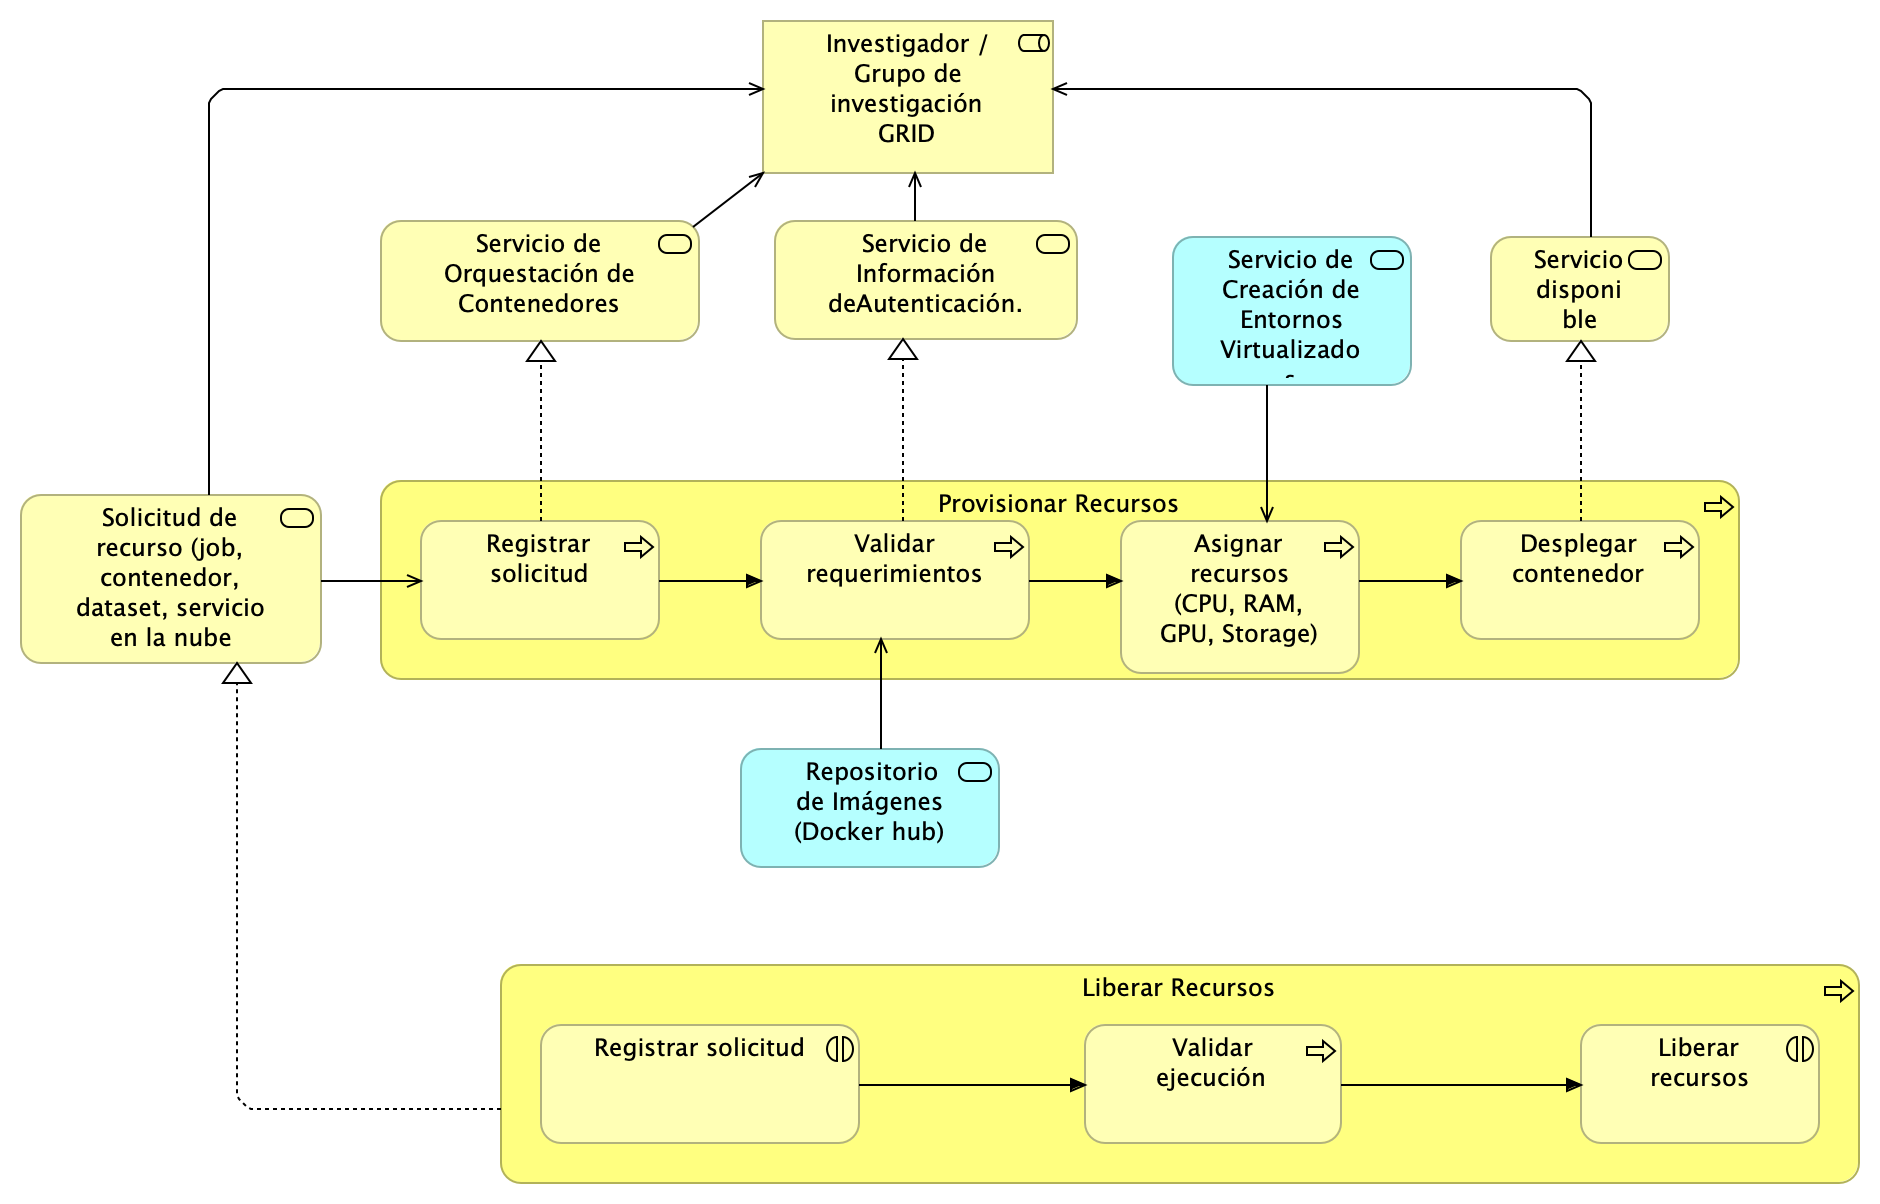
\includegraphics[width=\textwidth]{tablas-images/cp6/Business-Cooperation-View.png}
    \caption{Vista de Cooperación de Negocio}\label{fig:vista-cooperacion-negocio}
\end{figure}

El diagrama~\ref{fig:vista-productos-negocio} ilustra cómo los investigadores y estudiantes acceden a los recursos de cómputo bajo un marco regulado por políticas de uso y respaldado por un SLA. Muestra el flujo desde la solicitud hasta la ejecución de los contenedores, buscando la trazabilidad y control en el consumo de infraestructura.

\begin{figure}[H]
    \centering
    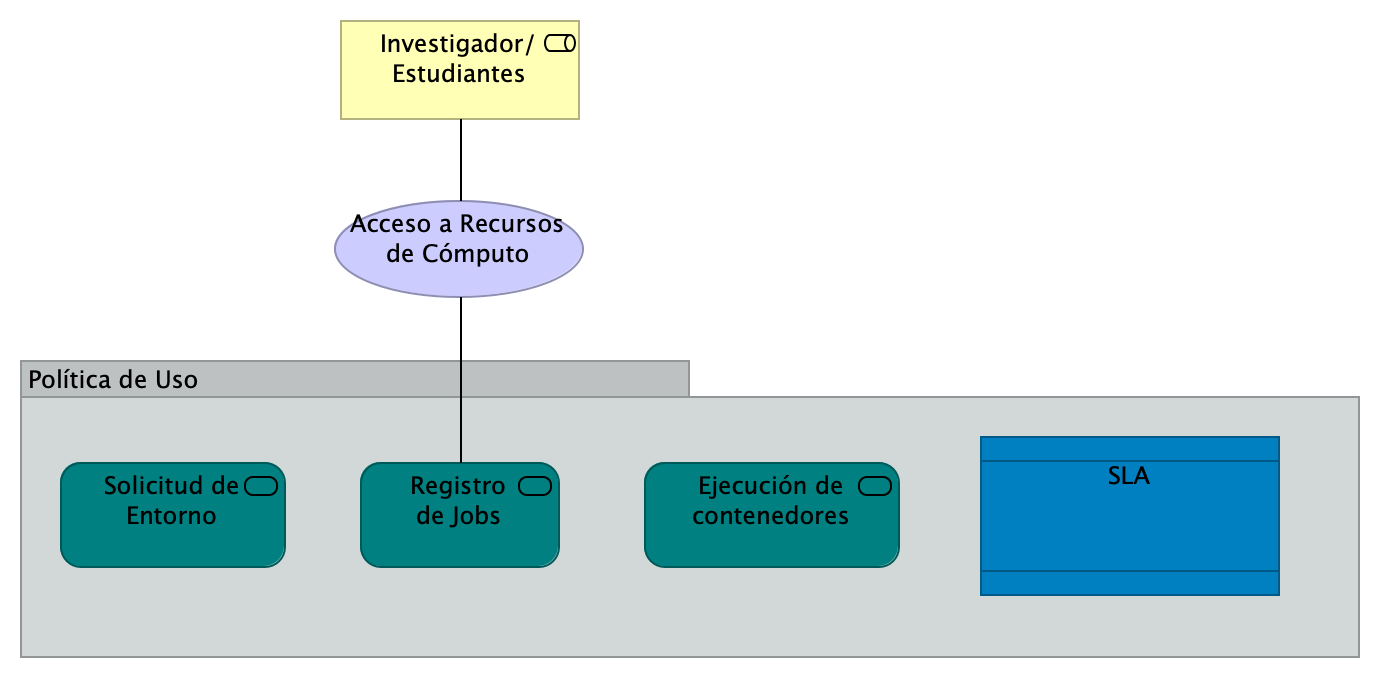
\includegraphics[width=\textwidth]{tablas-images/cp6/Business-Product-View.png}
    \caption{Vista de Producto de Negocio}\label{fig:vista-productos-negocio}
\end{figure}


La imagen~\ref{fig:vista-proceso-negocio} muestra el ciclo de vida completo de los entornos de cómputo: desde la solicitud de ejecución por parte de investigadores o estudiantes, pasando por el registro, validación, planificación de recursos y despliegue, hasta la liberación de los recursos una vez usados. En este flujo intervienen componentes clave como descriptores de jobs en Kubernetes, credenciales de clúster, registros de usuario, acuerdos de recursos, autenticación, orquestador y scheduler de prioridad. En conjunto, el modelo refleja cómo se gestionan de manera controlada y auditable los recursos computacionales dentro del sistema.
\begin{figure}[H]
    \centering
    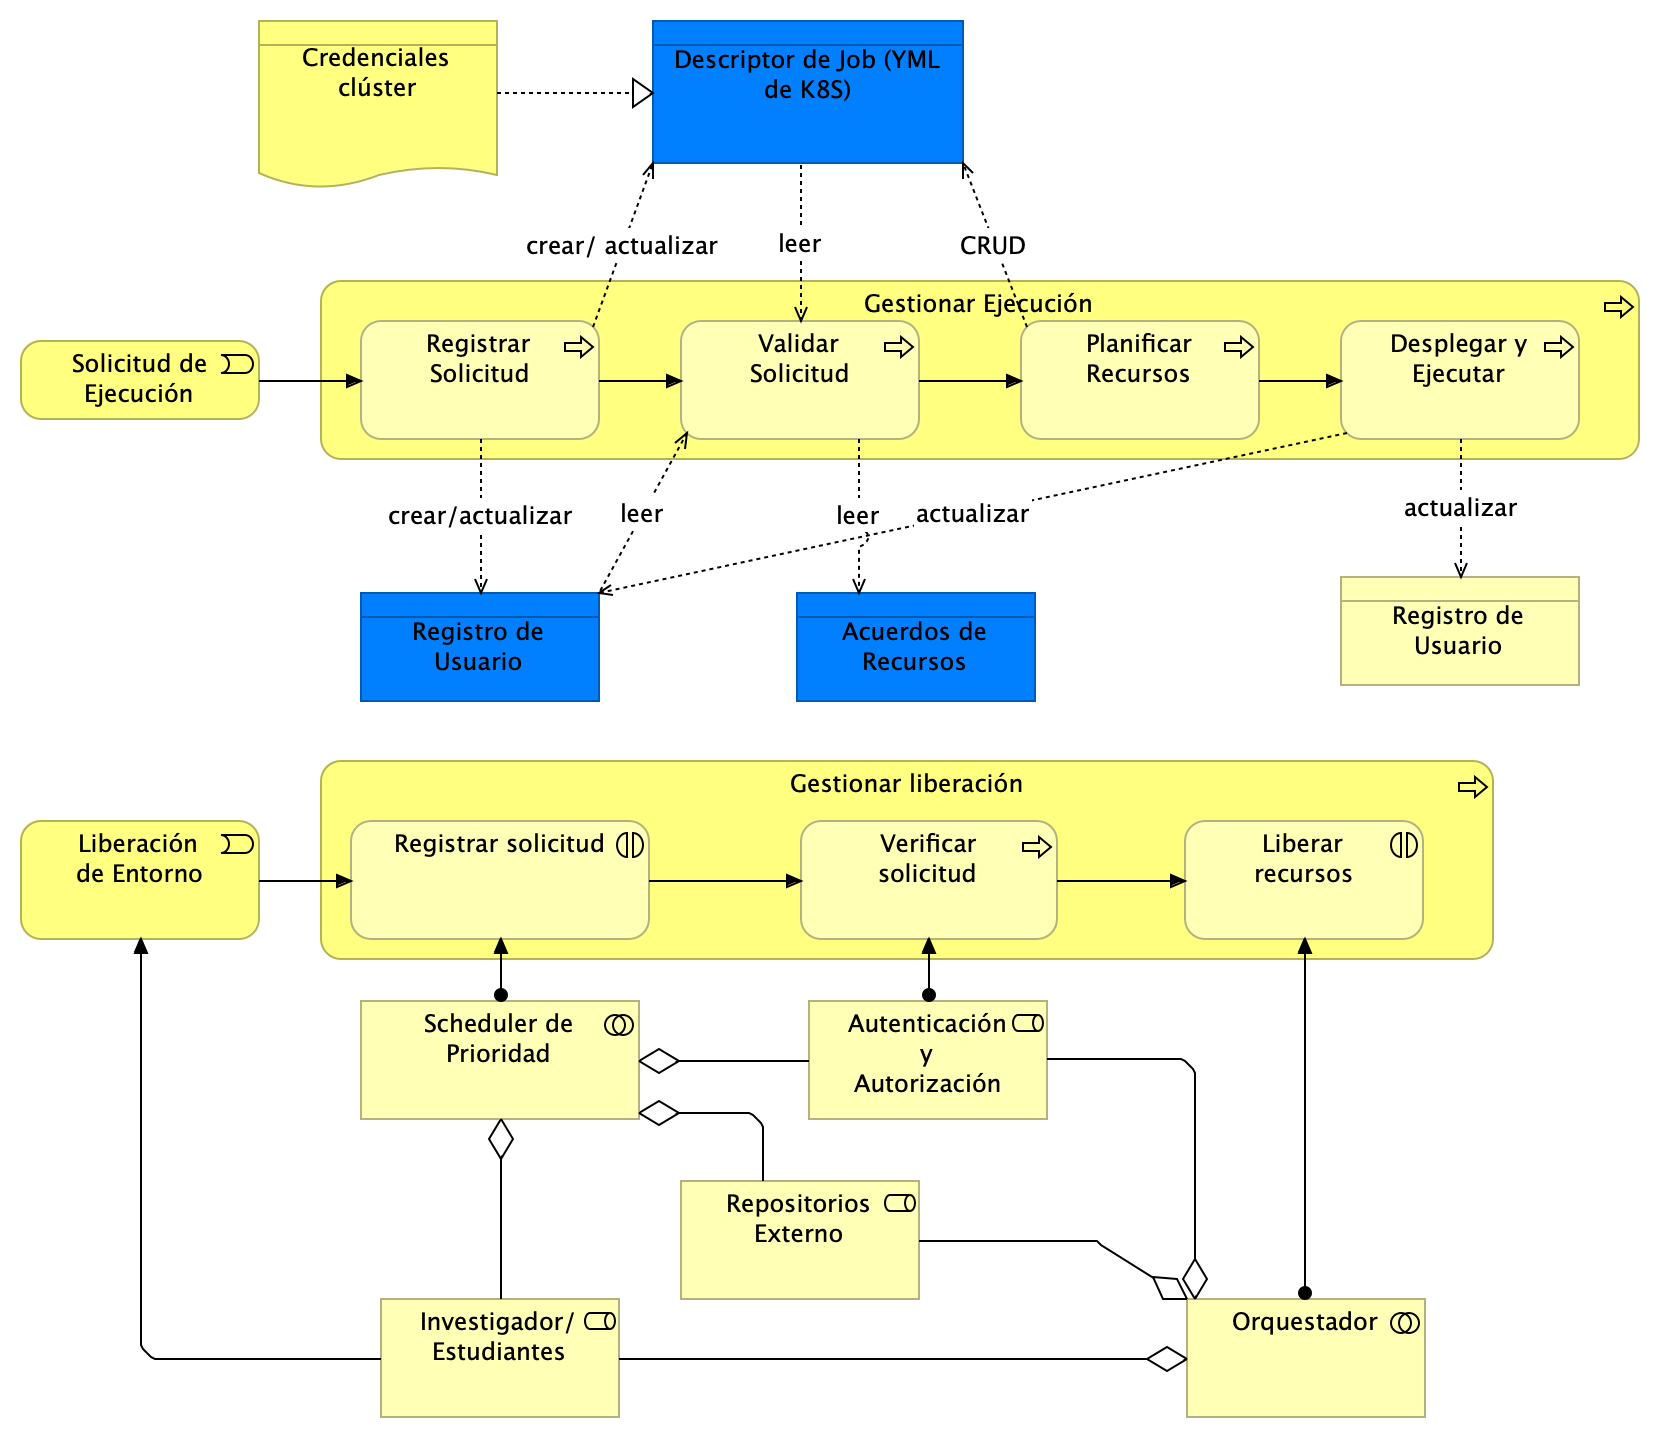
\includegraphics[width=\textwidth]{tablas-images/cp6/Business-Process-View.png}
    \caption{Vista de Proceso de Negocio}\label{fig:vista-proceso-negocio}
\end{figure}

El diagrama ~\ref{fig:vista-funcion-negocio}  muestra cómo la solución de virtualización basada en contenedores del GRID organiza sus principales funciones para dar soporte a estudiantes e investigadores. Entre ellas destacan la gestión de colaboraciones externas, la orquestación de recursos, la gestión de infraestructura virtualizada, la gestión de recursos de cómputo y consumo, la gestión de ejecuciones y la gestión de estudiantes e investigadores. El diagrama refleja la interacción entre actores clave (GRID, estudiantes/investigadores y datacenter Ingesis), señalando el flujo de información, el uso de infraestructura y los resultados de proyectos, lo que permite una administración integral  y alineada con los objetivos académicos y de investigación.

\begin{figure}[H]
    \centering
    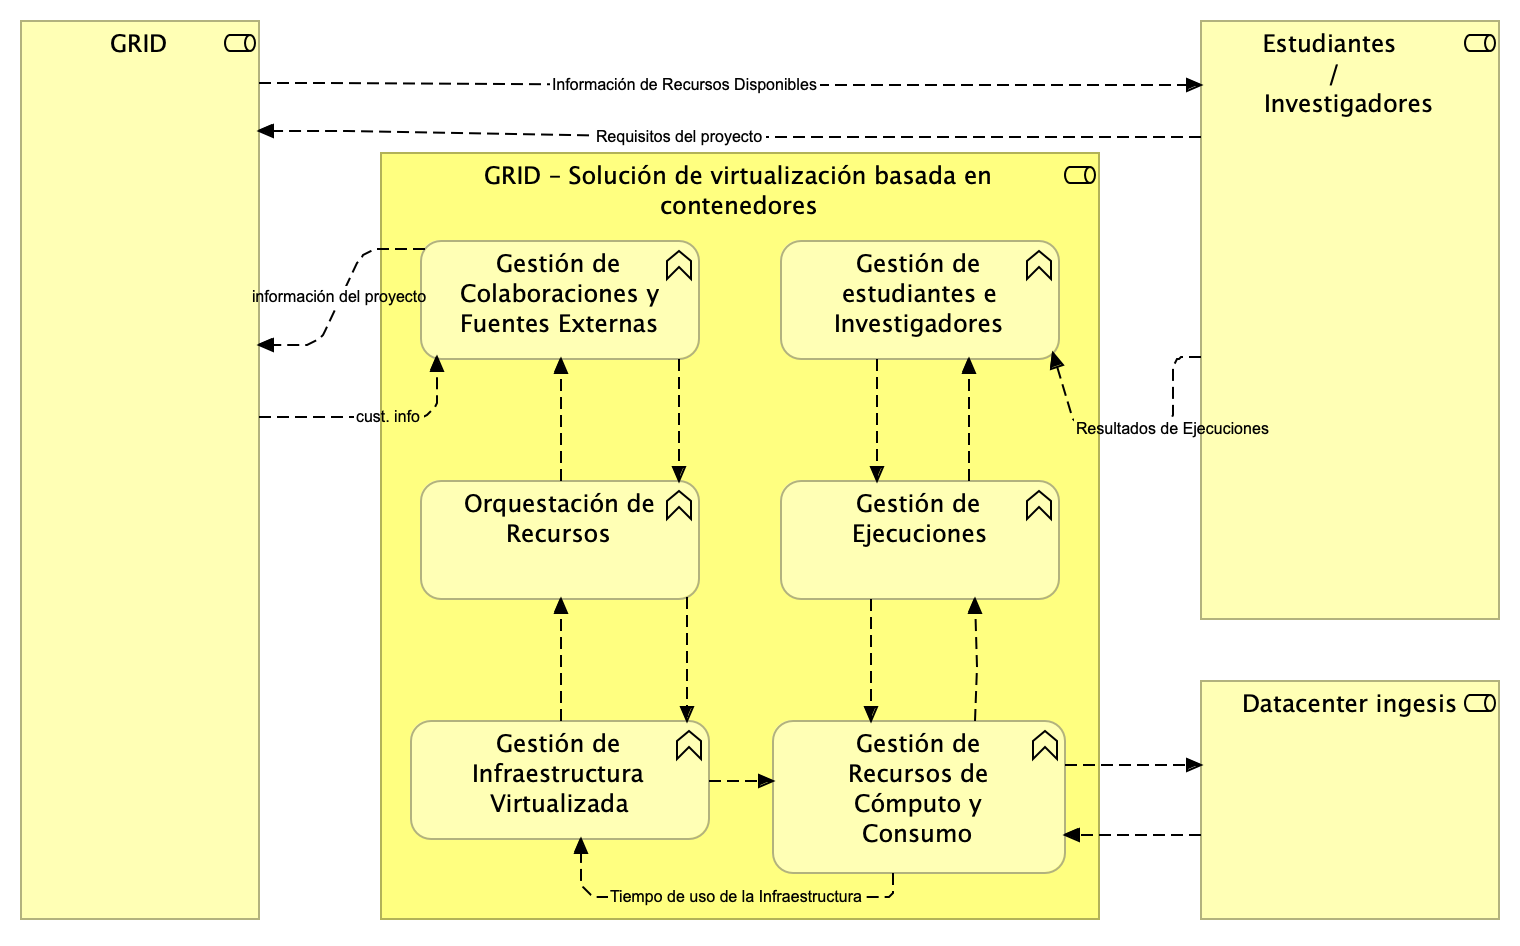
\includegraphics[width=\textwidth]{tablas-images/cp6/Business-Function-View.png}
    \caption{Vista de Función de Negocio}\label{fig:vista-funcion-negocio}
\end{figure}

\subsection{Vista de aplicación}
\begin{figure}[H]
    \centering
    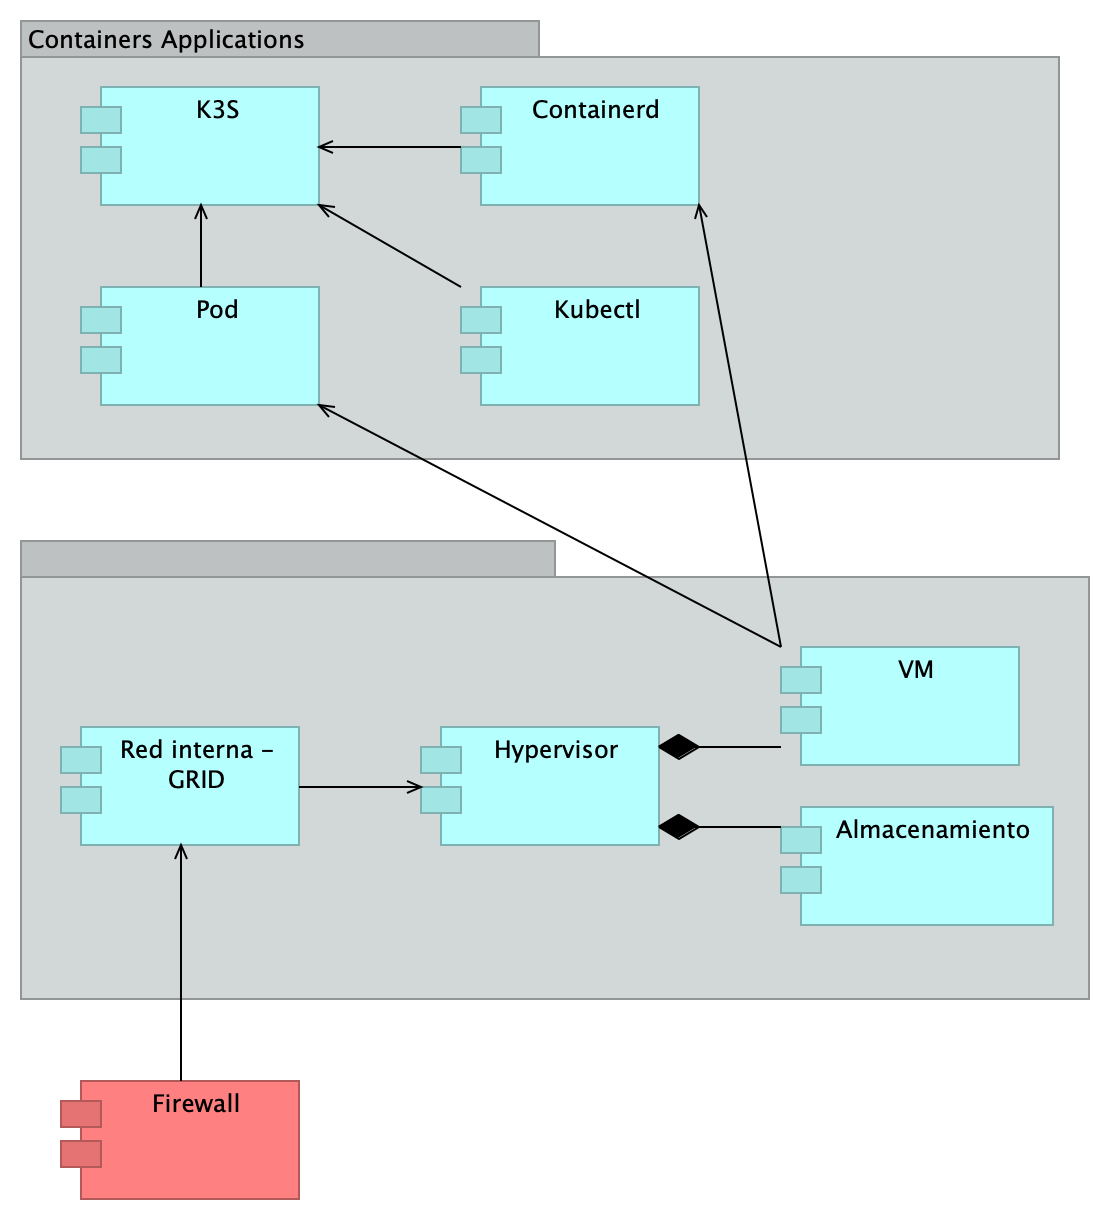
\includegraphics[width=\textwidth]{tablas-images/cp6/Application-Cooperation-View.png}
    \caption{Vista de Cooperación de Aplicaciones}
\end{figure}
\begin{figure}[H]
    \centering
    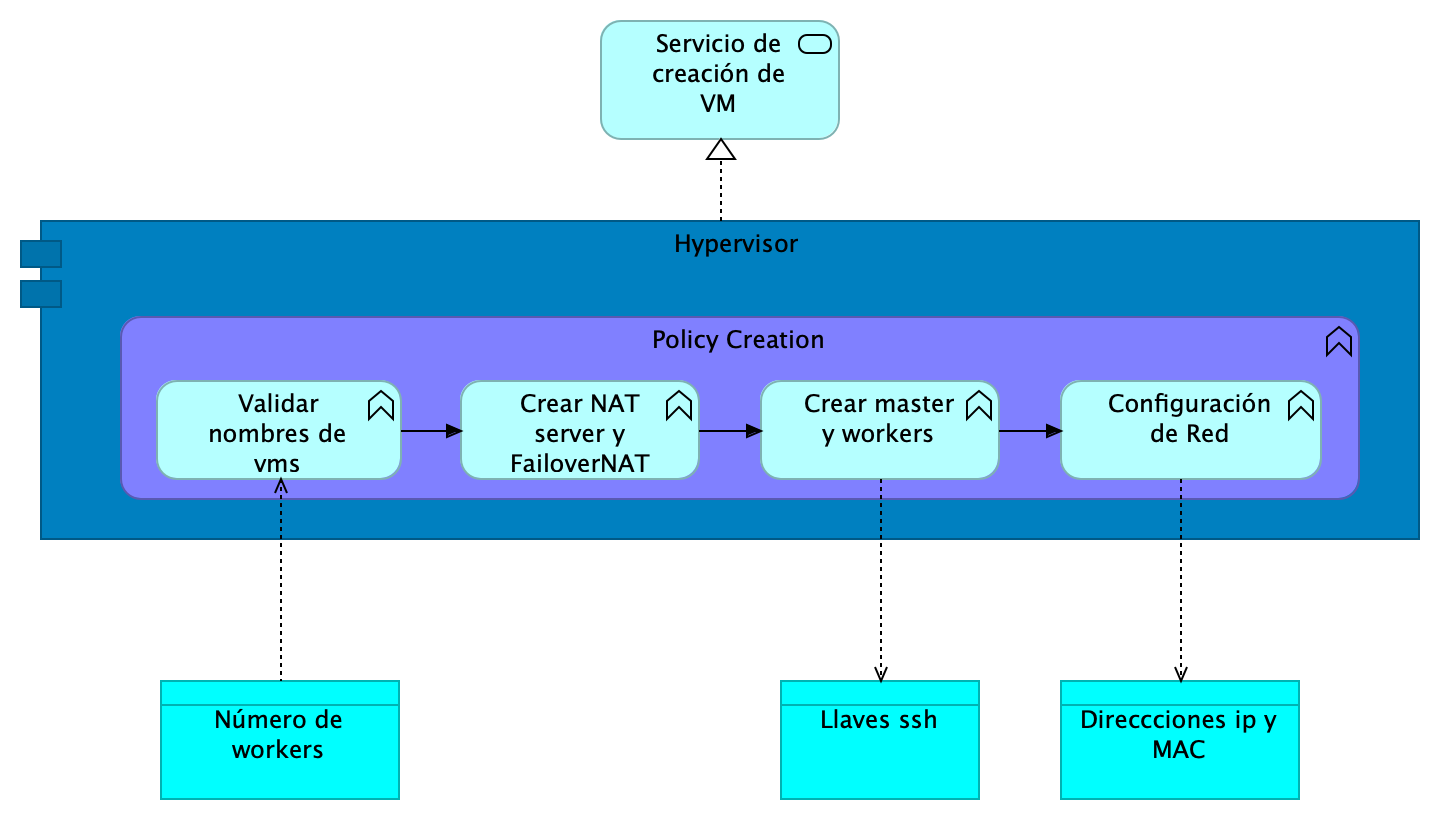
\includegraphics[width=\textwidth]{tablas-images/cp6/Application-Behaviour-view.png}
    \caption{Vista de Comportamiento de Aplicaciones}
\end{figure}
\begin{figure}[H]
    \centering
    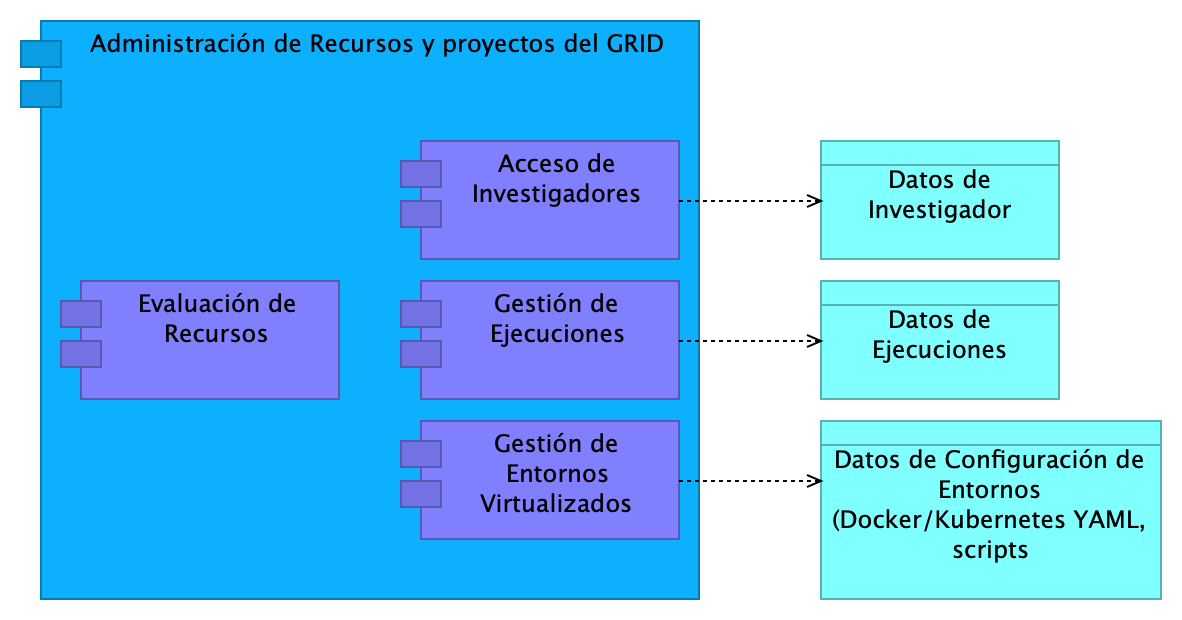
\includegraphics[width=\textwidth]{tablas-images/cp6/Application-Structure-View.png}
    \caption{Vista de Estructura de Aplicaciones}
\end{figure}

\subsection{Vista de tecnología}
\begin{figure}[H]
    \centering
    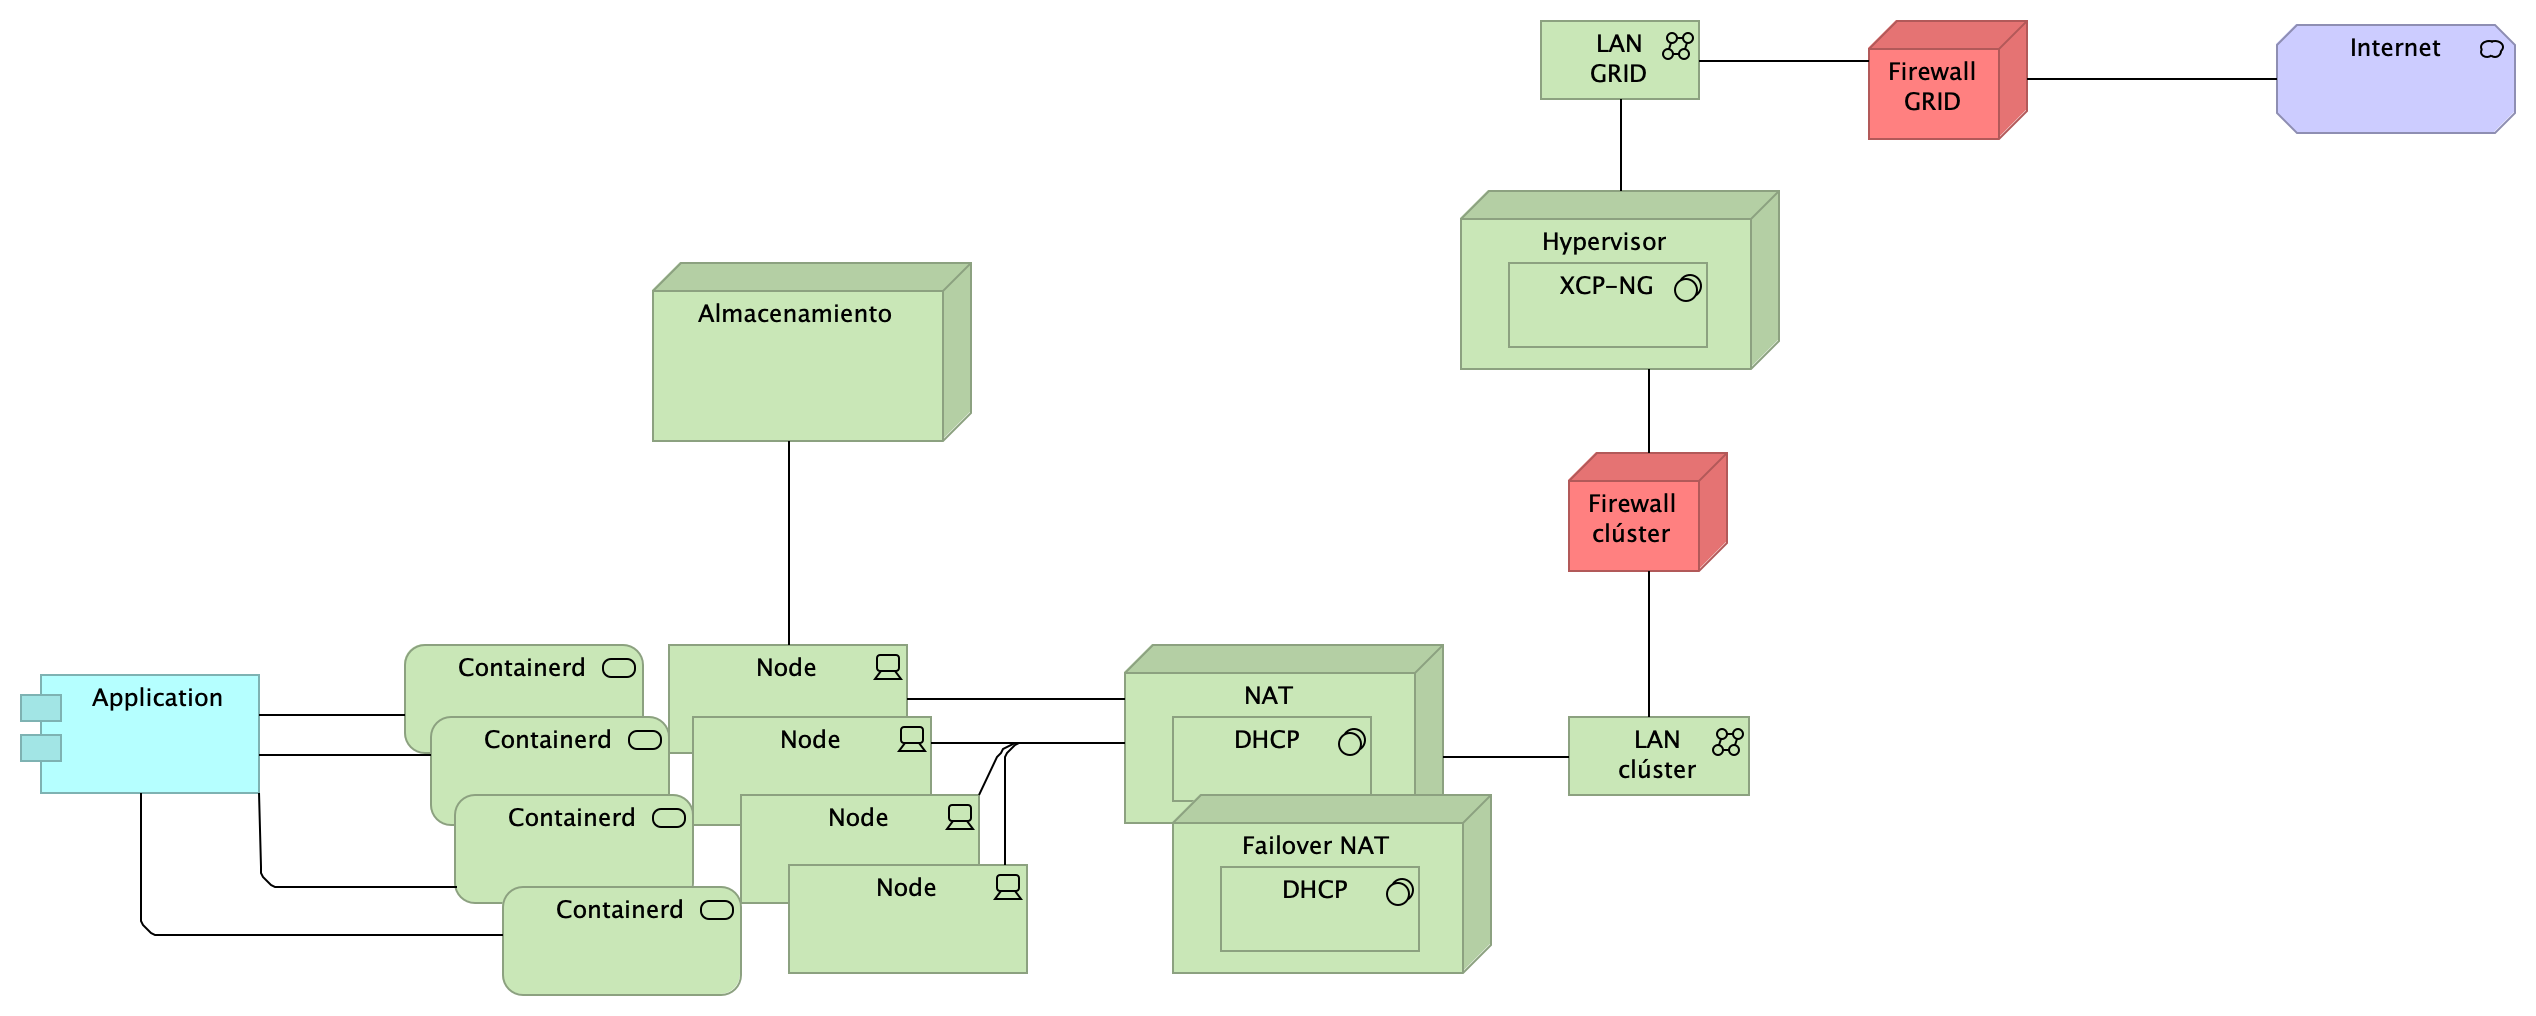
\includegraphics[width=\textwidth]{tablas-images/cp6/Implementation-and-Installation-View.png}
    \caption{Vista de Implementación e Instalación}
\end{figure}
\begin{figure}[H]
    \centering
    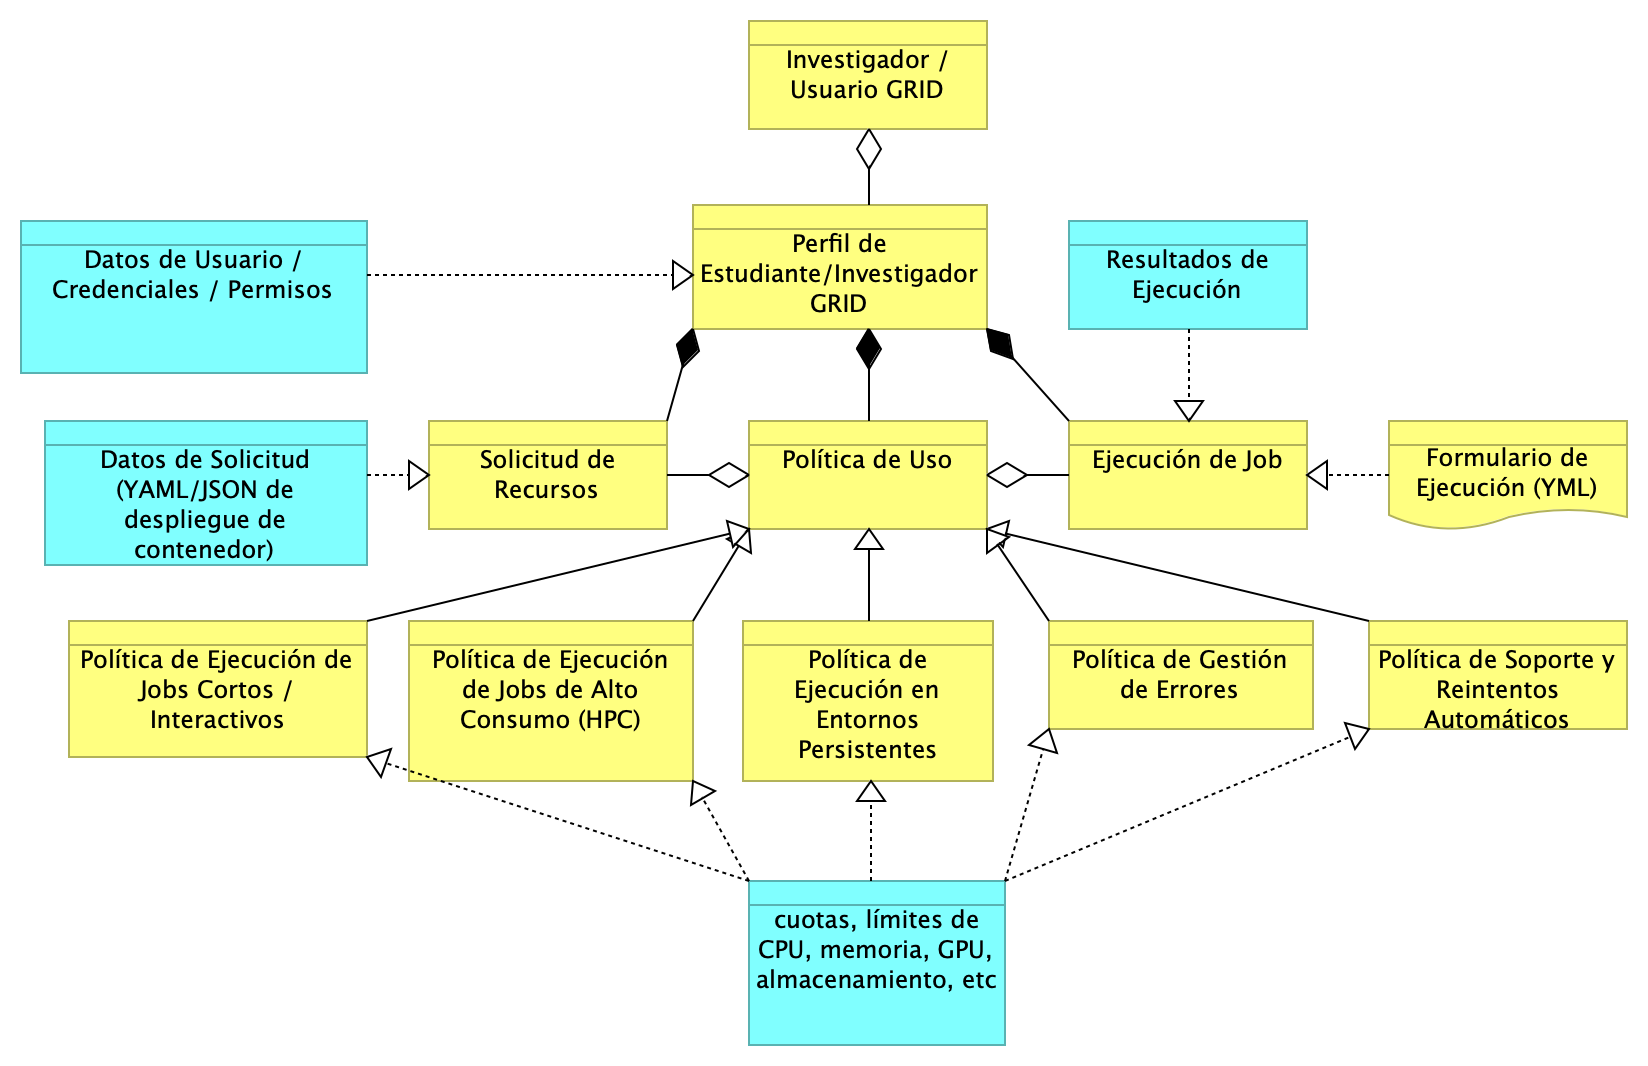
\includegraphics[width=\textwidth]{tablas-images/cp6/Information-Structure-View.png}
    \caption{Vista de Estructura de Información}
\end{figure}x


\subsection{Vista general}
% Vista general - Placeholder
% Este archivo contiene la vista general del modelo ArchiMate

\begin{figure}[H]
	\centering
	
\includegraphics[width=\textwidth]{images/placeholder.png}
	\caption{Vista general del sistema}
	\label{fig:vista-general}
\end{figure}

% Descripción de la vista general
La vista general integra las tres capas del modelo ArchiMate (negocio, aplicación y tecnología) para proporcionar una perspectiva completa de la arquitectura de la solución. Esta vista permite visualizar las relaciones y dependencias entre los diferentes elementos del sistema HTCondor, desde los procesos de negocio hasta la infraestructura tecnológica que los soporta.

Esta vista consolidada facilita la comprensión del sistema en su totalidad y sirve como herramienta de comunicación entre los diferentes stakeholders del proyecto, permitiendo identificar puntos de integración críticos y oportunidades de optimización en toda la arquitectura.


\section{Diseño por capas de la solución}

\section{Capa de infraestructura}

\begin{figure}[H]
    \centering
    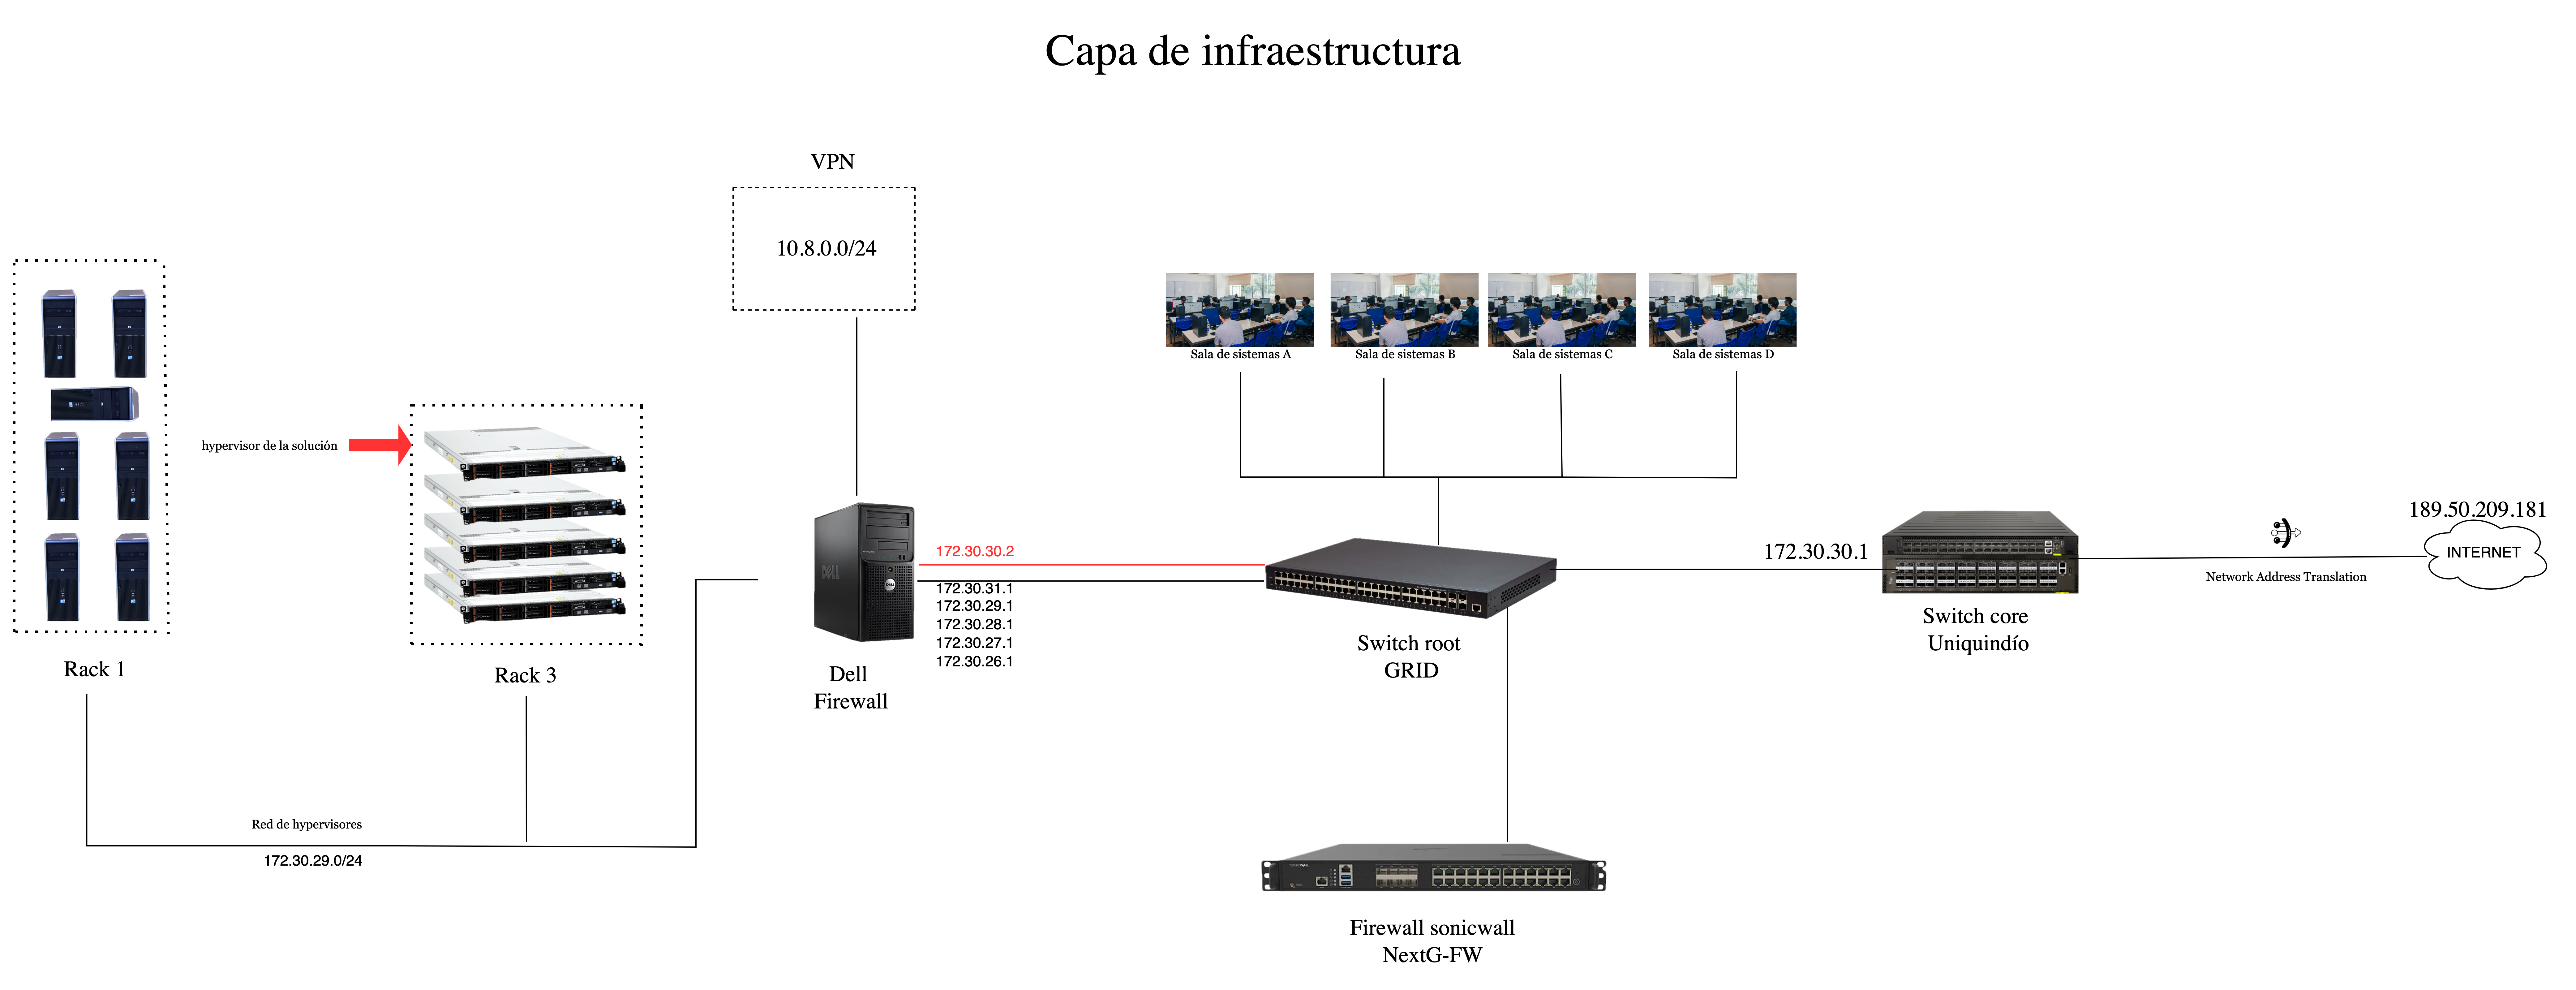
\includegraphics[width=\textwidth]{tablas-images/cp6/disenio-N1.png}
    \caption{Capa de Infraestructura}
\end{figure}

\section{Capa de virtualización}

\begin{figure}[H]
    \centering
    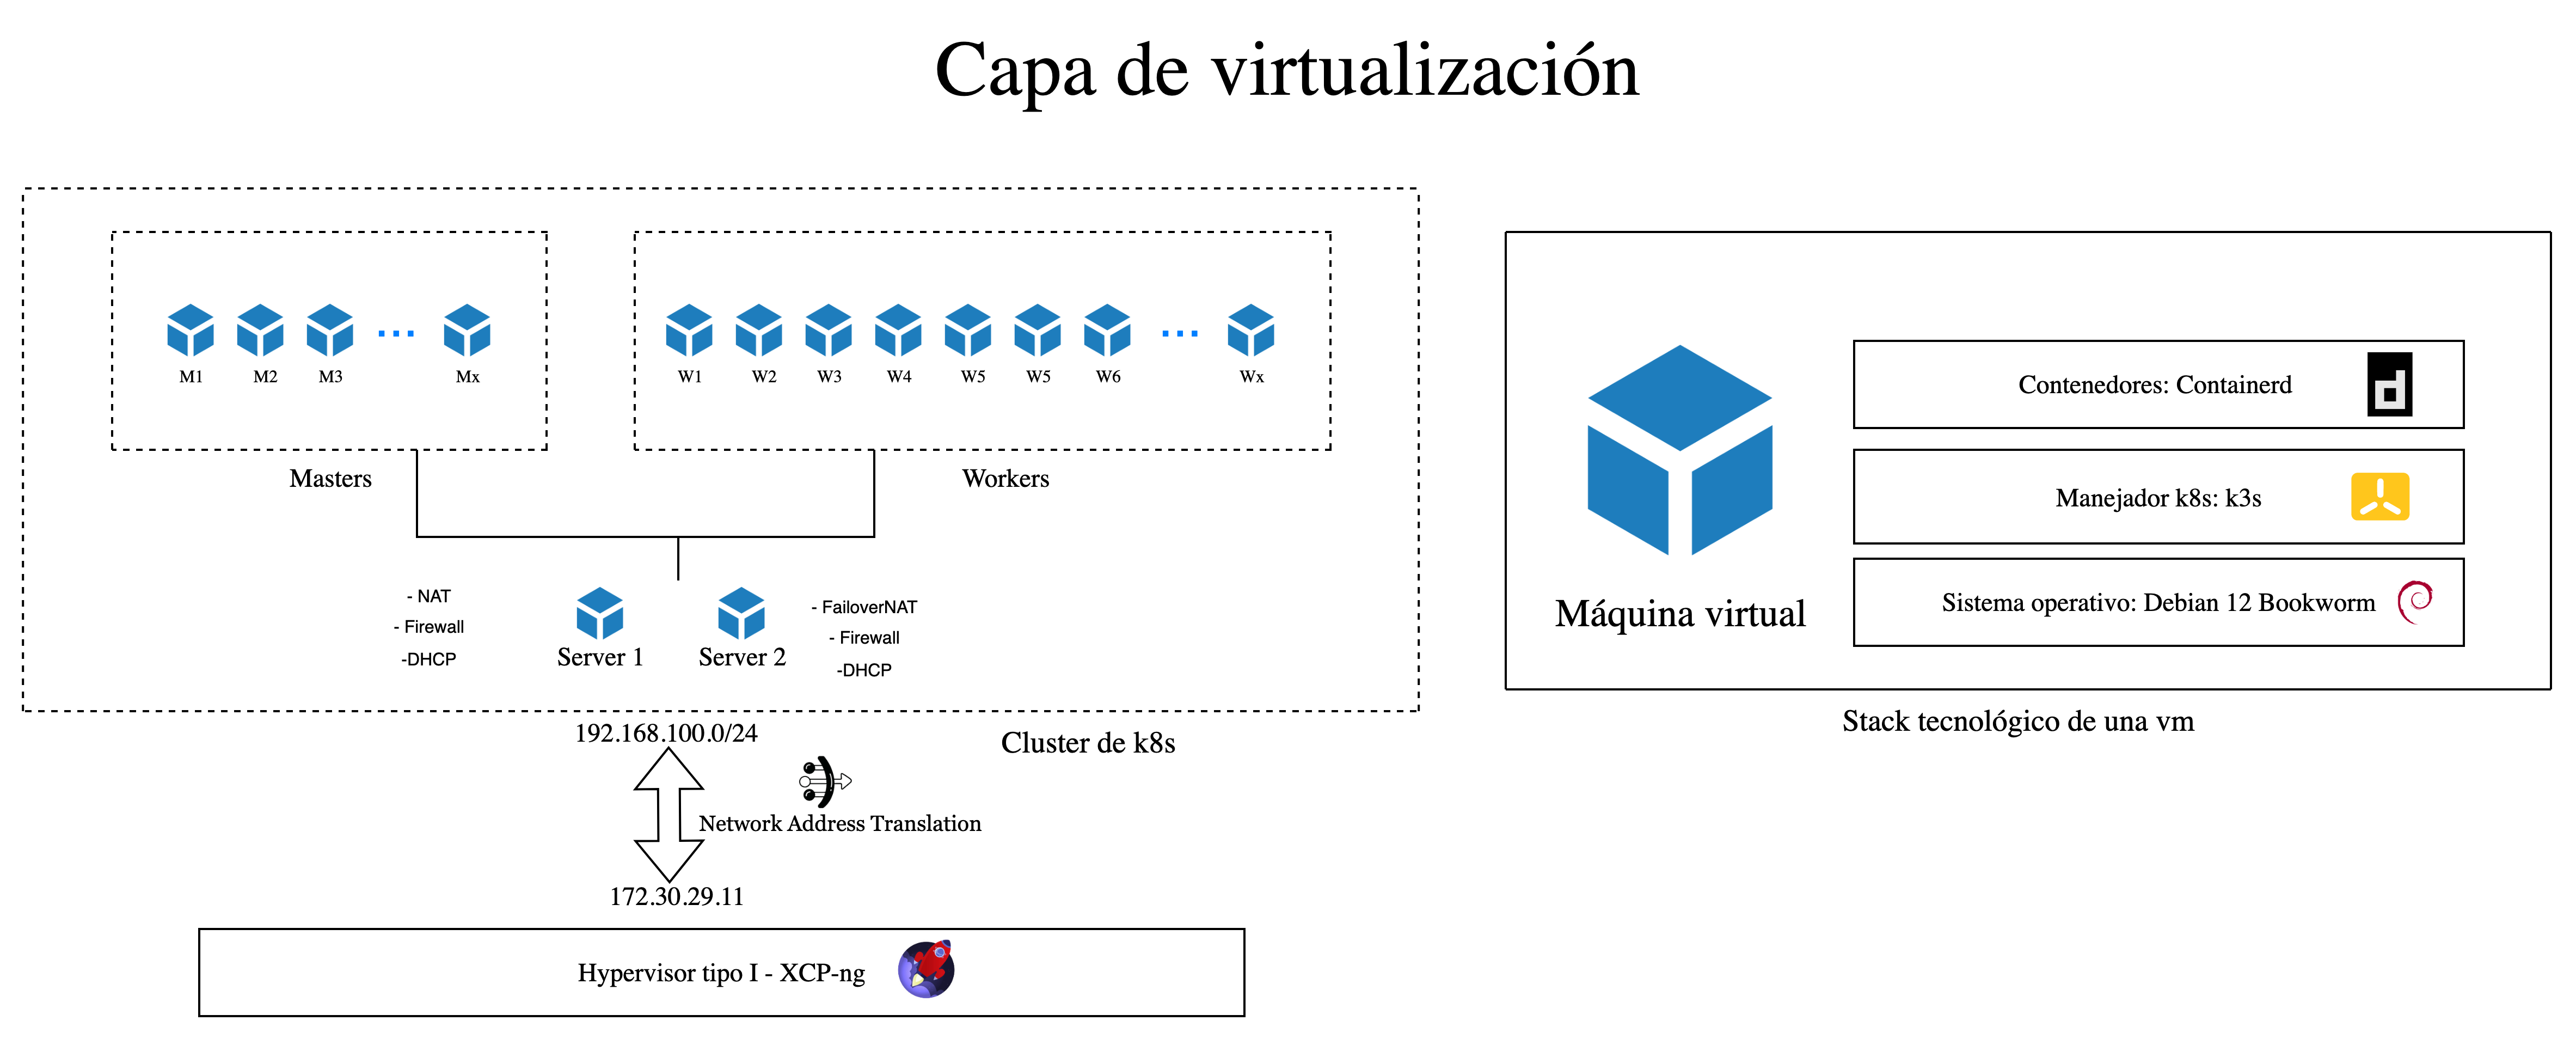
\includegraphics[width=\textwidth]{tablas-images/cp6/disenio-N2.png}
    \caption{Capa de Virtualización}
\end{figure}

\section{Capa de aplicación}


%\ChapterImageStar[cap:resultados]{Resultados}{./images/fondo.png}\label{cap:resultados}
\mbox{}\\
El desarrollo de esta investigación permitió obtener una serie de resultados tangibles y analíticos que responden a los objetivos planteados y contribuyen a la especificación de una solución arquitectónica basada en tecnologías de virtualización por contenedores (VBC) para el Grupo de Investigación en Redes, Información y Distribución (GRID) de la Universidad del Quindío. A continuación, se presentan los hallazgos más relevantes organizados según las fases metodológicas ejecutadas. En primer lugar, la caracterización del GRID permitió identificar sus capacidades tecnológicas actuales, su misión institucional y las necesidades específicas de sus stakeholders. Se determinó que el grupo cuenta con una infraestructura de virtualización basada en el hipervisor XCP-ng, compuesta por servidores tipo torre y rack, con especificaciones técnicas heterogéneas pero suficientes para soportar servicios educativos y de investigación. No obstante, se evidenció la necesidad de incorporar instancias computacionales más ligeras y eficientes que complementen la infraestructura existente y amplíen la oferta de servicios hacia la comunidad académica, en particular para los estudiantes de Ingeniería de Sistemas y Computación. El análisis de stakeholders permitió priorizar a los integrantes del GRID, docentes y estudiantes como actores clave, lo cual orientó el diseño de la solución hacia sus necesidades reales. La revisión sistemática de la literatura (SMS) arrojó como resultado la identificación y clasificación de 18 tecnologías VBC relevantes en el ámbito académico y profesional. Mediante una estrategia de búsqueda en bases de datos académicas y la técnica de bola de nieve, se seleccionaron y analizaron 116 estudios que permitieron construir un panorama actualizado del estado del arte. Tecnologías como Docker, Podman, LXC, Containerd, LXD, Singularity, Wasm, entre otras, fueron caracterizadas en términos de licencias, interfaces de uso, integración con nubes públicas, entornos de ejecución y adopción en la industria. La aplicación de un cuadrante Gartner permitió visualizar la posición relativa de cada tecnología, situando a Docker y Containerd en el cuadrante de líderes, mientras que otras como Udocker o Sarus se ubicaron como jugadores de nicho, orientados a entornos específicos como HPC. El benchmarking técnico realizado sobre un subconjunto de tecnologías preseleccionadas —Docker, Podman, LXC, LXD y Containerd— proporcionó mediciones objetivas de rendimiento en condiciones controladas. Los resultados mostraron diferencias significativas en el consumo de recursos, tiempo de arranque, throughput de red y latencia de E/S. Containerd destacó por su eficiencia general, con un bajo consumo de CPU (99.71\% de tiempo en idle), un tiempo de arranque rápido y una latencia de disco reducida. LXC, por su parte, mostró el menor consumo de memoria RAM (2.835\%) y el mejor desempeño en throughput de red, aunque con un tiempo de arranque superior. Podman, si bien eficiente en recursos, presentó limitaciones en el rendimiento de red y E/S. Estos resultados proporcionaron una base cuantitativa para la toma de decisiones subsiguiente. El Análisis de Decisiones y Resolución (DAR), aplicado conforme al modelo CMMI, permitió evaluar las tecnologías VBC con base en 12 criterios técnicos y organizacionales, entre los que se incluyeron: tipo de licencia, posibilidad de orquestación, compatibilidad con Docker Hub, soporte para redes personalizadas, persistencia de datos, documentación, soporte comunitario, popularidad, consumo de recursos, compatibilidad con orquestadores y costos de implementación. Containerd obtuvo la puntuación más alta (233/300), destacando por su licencia Apache 2.0, integración nativa con Kubernetes, amplia documentación, bajo consumo de recursos y compatibilidad total con el ecosistema Docker. Adicionalmente, se evaluaron distintas alternativas de motores de orquestación para Kubernetes, donde K3S resultó seleccionado por su facilidad de instalación, bajo consumo de recursos y compatibilidad con entornos limitados en hardware. Con base en lo anterior, se diseñó una solución arquitectónica modelada en Archimate, que integra la infraestructura existente del GRID con una capa de virtualización basada en Containerd y K3S. El modelo incluye vistas de negocio, aplicación y tecnología, articulando procesos como la solicitud de entornos virtualizados, la provisión de recursos y la gestión de ejecuciones. Se propuso un modelo por capas que separa claramente la infraestructura física, la capa de virtualización (contenedores y orquestación) y la capa de aplicación, facilitando así el mantenimiento, la escalabilidad y la gestión de servicios. Finalmente, se implementó y validó un producto mínimo viable (PMV) que materializó la arquitectura propuesta. El PMV fue desplegado en un entorno controlado dentro de la infraestructura del GRID, permitiendo la ejecución de contenedores OCI gestionados mediante K3S y Containerd. La validación incluyó pruebas de funcionalidad, rendimiento y usabilidad, realizadas en colaboración con usuarios potenciales (investigadores y estudiantes). Los resultados de estas pruebas confirmaron que la solución es estable, reproducible y adecuada para su uso en escenarios académicos y de investigación, cumpliendo con los requerimientos identificados durante la caracterización inicial. En conjunto, estos resultados demuestran que la incorporación de Containerd y K3S en la infraestructura del GRID representa una alternativa viable y eficiente para expandir su portafolio de servicios mediante contenedores, sin desestimar la inversión previa en virtualización tradicional. La metodología aplicada —que combinó caracterización contextual, revisión sistemática, evaluación técnica y diseño arquitectónico— provee un marco reproducible para la selección e implementación de tecnologías VBC en contextos académicos con restricciones de recursos y alineados con misiones institucionales de docencia, investigación y extensión.
%\ChapterImageStar[cap:conclusiones]{Conclusiones}{./images/fondo.png}\label{cap:conclusiones}
\mbox{}\\
%\ChapterImageStar[cap:trabajos-futuros]{Trabajos Futuros}{./images/fondo.png}\label{cap:trabajos-futuros}
\mbox{}\\

%\ChapterImageStar[cap:cumplimiento-objetivos]{Cumplimiento de objetivos}{./images/fondo.png}\label{cap:cumplimiento-objetivos}



%% Referencias - con imagen de fondo específica
\cleardoublepage\thispagestyle{empty}
\refstepcounter{chapter}
\phantomsection\addcontentsline{toc}{chapter}{Referencias}\label{cap:referencias}

% Imagen de fondo específica para referencias
\AddToShipoutPicture*{%
	\put(0,0){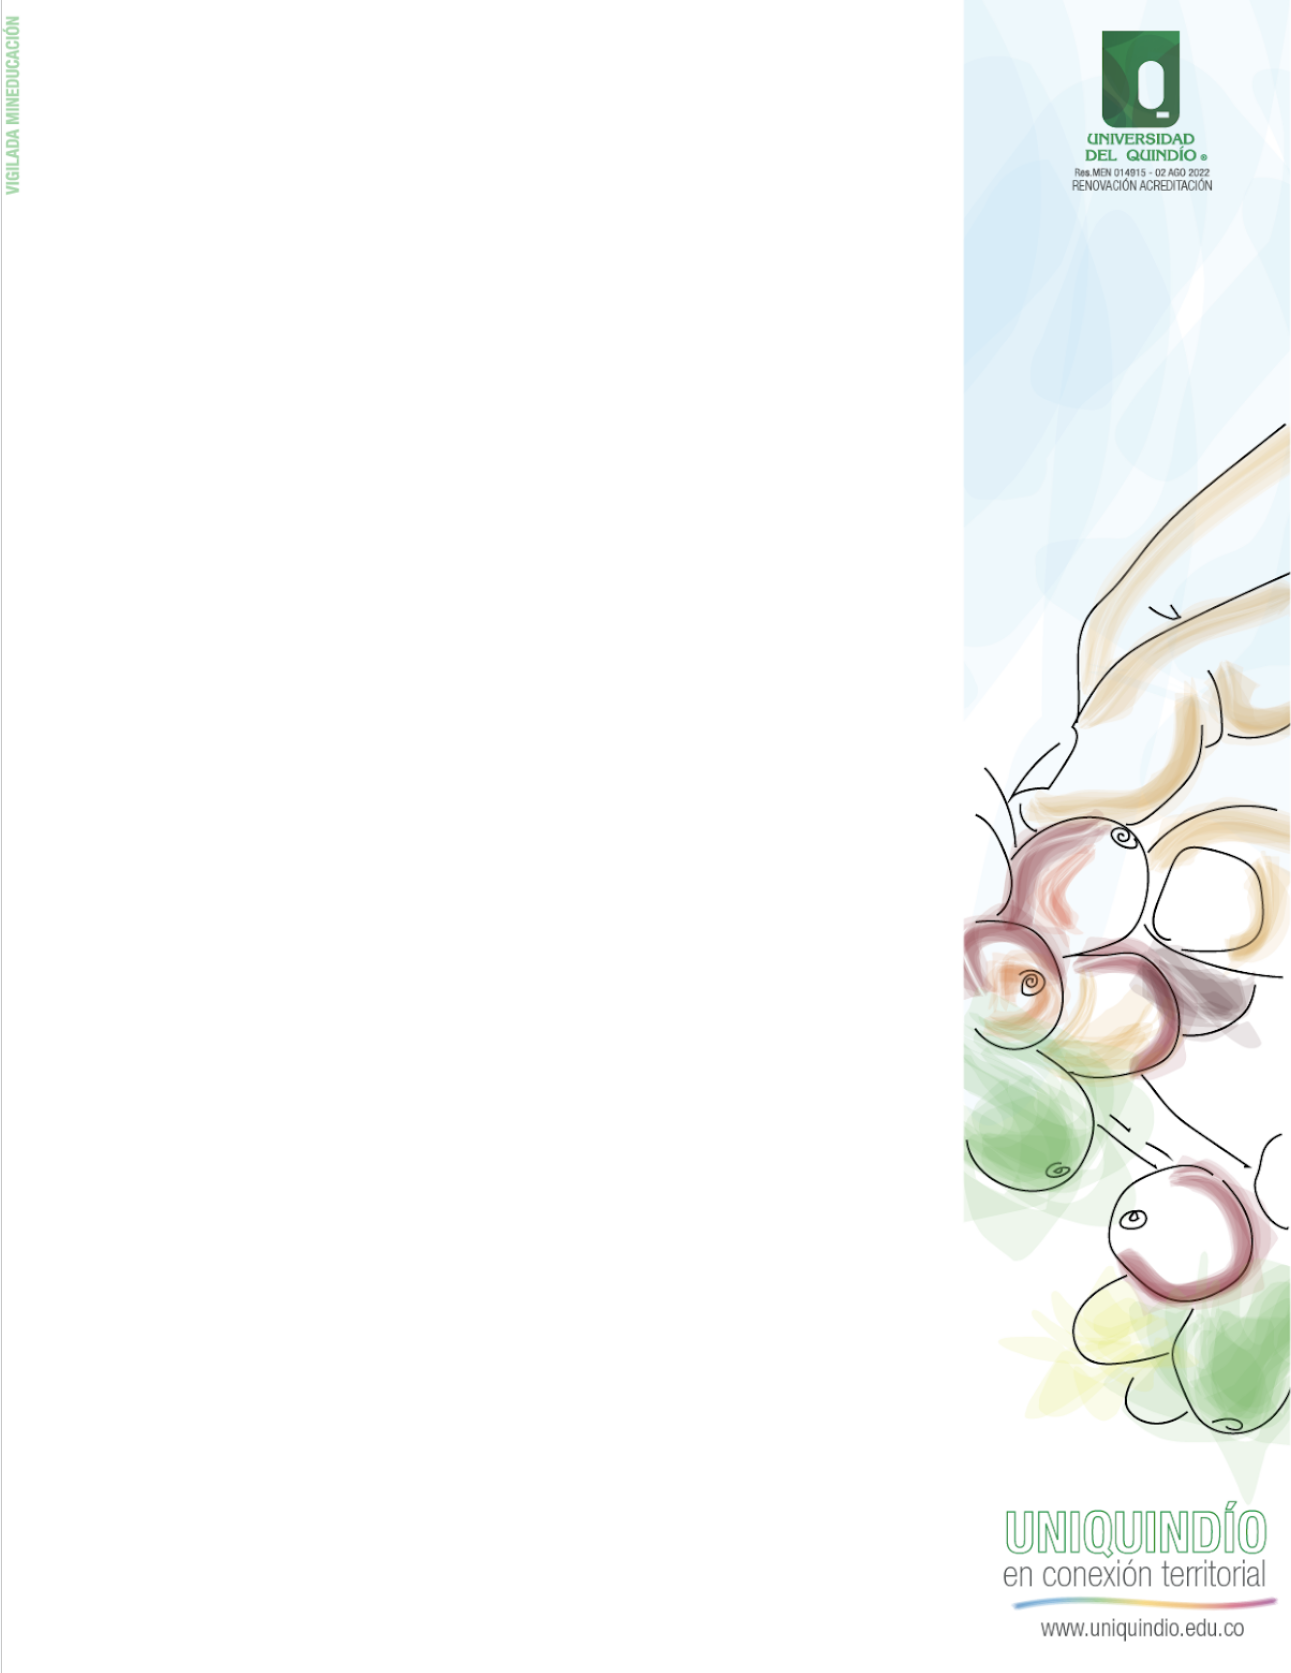
\includegraphics[width=\paperwidth,height=\paperheight]{./images/referencias.png}}%
}

% Título posicionado con coordenadas absolutas (en píxeles desde esquina superior izquierda)
\begin{tikzpicture}[remember picture,overlay]
	\node[anchor=north west] at ([xshift=150pt,yshift=-370pt]current page.north west)
	{\Large\bfseries\textcolor{black}{Referencias}};
\end{tikzpicture}
\vspace{2cm}

% Bibliografía sin título automático
\begingroup
\renewcommand{\bibname}{}
\pagestyle{fancy} % Fuerza el estilo fancy para todas las páginas de bibliografía
\bibliographystyle{apalike}
\bibliography{bibliografia}
\endgroup

%\appendix

% CHAPTER Búsquedas en bases de datos

\phantomsection

% Increment the chapter counter so \thechapter shows the correct number
% and make it referenceable with \ref
\refstepcounter{chapter}

% Manually add this appendix to the Table of Contents
\addcontentsline{toc}{chapter}{Apéndice \thechapter: Búsqueda en bases de datos}

% Add vertical space above the title (mimics standard chapter spacing)
\vspace{40pt}

% Display the actual chapter title (centered, large, bold)
{\centering \normalfont\huge\bfseries Apéndice~\thechapter: Búsqueda en bases de datos~\par}

% Add spacing between title and horizontal rule
\vspace{10pt}

% Draw a horizontal line across the page for visual separation
{\centering \rule{\textwidth}{0.4pt} \par}

% Add vertical space between title section and content
\vspace{40pt}

% Set the running headers for left and right pages
\markboth{Apéndice \thechapter:Búsqueda en bases de datos}{Apéndice \thechapter: Búsqueda en bases de datos}



\FloatBarrier\section{Cadenas de búsqueda}\label{sec:cadenas-busqueda}


\begin{tcolorbox}[
		colback=gray!5,
		colframe=black!60,
		title=Cadena de búsqueda en ACM Full Text Collection,
		fonttitle=\bfseries,
		sharp corners=south
	]
	\scriptsize
	\begin{verbatim}
((HTCondor OR Condor) AND (HTC OR "High Throughput Computing" OR HPC OR "High
Performance Computing") AND (Universe OR "Execution Environment") AND (Project OR
Work) AND (Research OR Teaching OR Industry))
	\end{verbatim}
\end{tcolorbox}

\begin{tcolorbox}[
		colback=gray!5,
		colframe=black!60,
		title=Cadena de búsqueda en IEEE Xplore,
		fonttitle=\bfseries,
		sharp corners=south
	]
	\scriptsize
	\begin{verbatim}
(HTCondor OR Condor) AND (HTC OR (High Throughput Computing)) AND (Universe OR
(Runtime Environment)) AND (Research OR Teaching OR Industry)
	\end{verbatim}
\end{tcolorbox}

\begin{tcolorbox}[
		colback=gray!5,
		colframe=black!60,
		title=Cadena de búsqueda en Springer,
		fonttitle=\bfseries,
		sharp corners=south
	]
	\scriptsize
	\begin{verbatim}
((HTCondor — Condor) + (HTC — "High Throughput Computing" — HPC — "High
Performance Computing") + (Universe — "Execution Environment") + (Project — Work) +
(Research — Teaching — Industry))
	\end{verbatim}
\end{tcolorbox}

\begin{tcolorbox}[
		colback=gray!5,
		colframe=black!60,
		title=Cadena de búsqueda en ScienceDirect,
		fonttitle=\bfseries,
		sharp corners=south
	]
	\scriptsize
	\begin{verbatim}
(HTCondor OR Condor) (HTC OR "High Throughput Computing" OR HPC OR "High Performance Computing") (Universe OR "Execution Environment") (Project OR Work) (Research OR
Teaching OR Industry)
	\end{verbatim}
\end{tcolorbox}

\begin{tcolorbox}[
		colback=gray!5,
		colframe=black!60,
		title=Cadena de búsqueda en Taylor \& Francis,
		fonttitle=\bfseries,
		sharp corners=south
	]
	\scriptsize
	\begin{verbatim}
(HTCondor OR Condor) AND (HTC OR (High Throughput Computing)) AND (Universe OR
(Runtime Environment)) AND (Research OR Teaching OR Industry)
  \end{verbatim}
\end{tcolorbox}


\section{Búsqueda de artículos sin criterios de inclusión/exclusión}\label{sec:busqueda-sin-criterios}

% ##### Imagenes de busqueda ########

\begin{figure}[H]
	\centering
	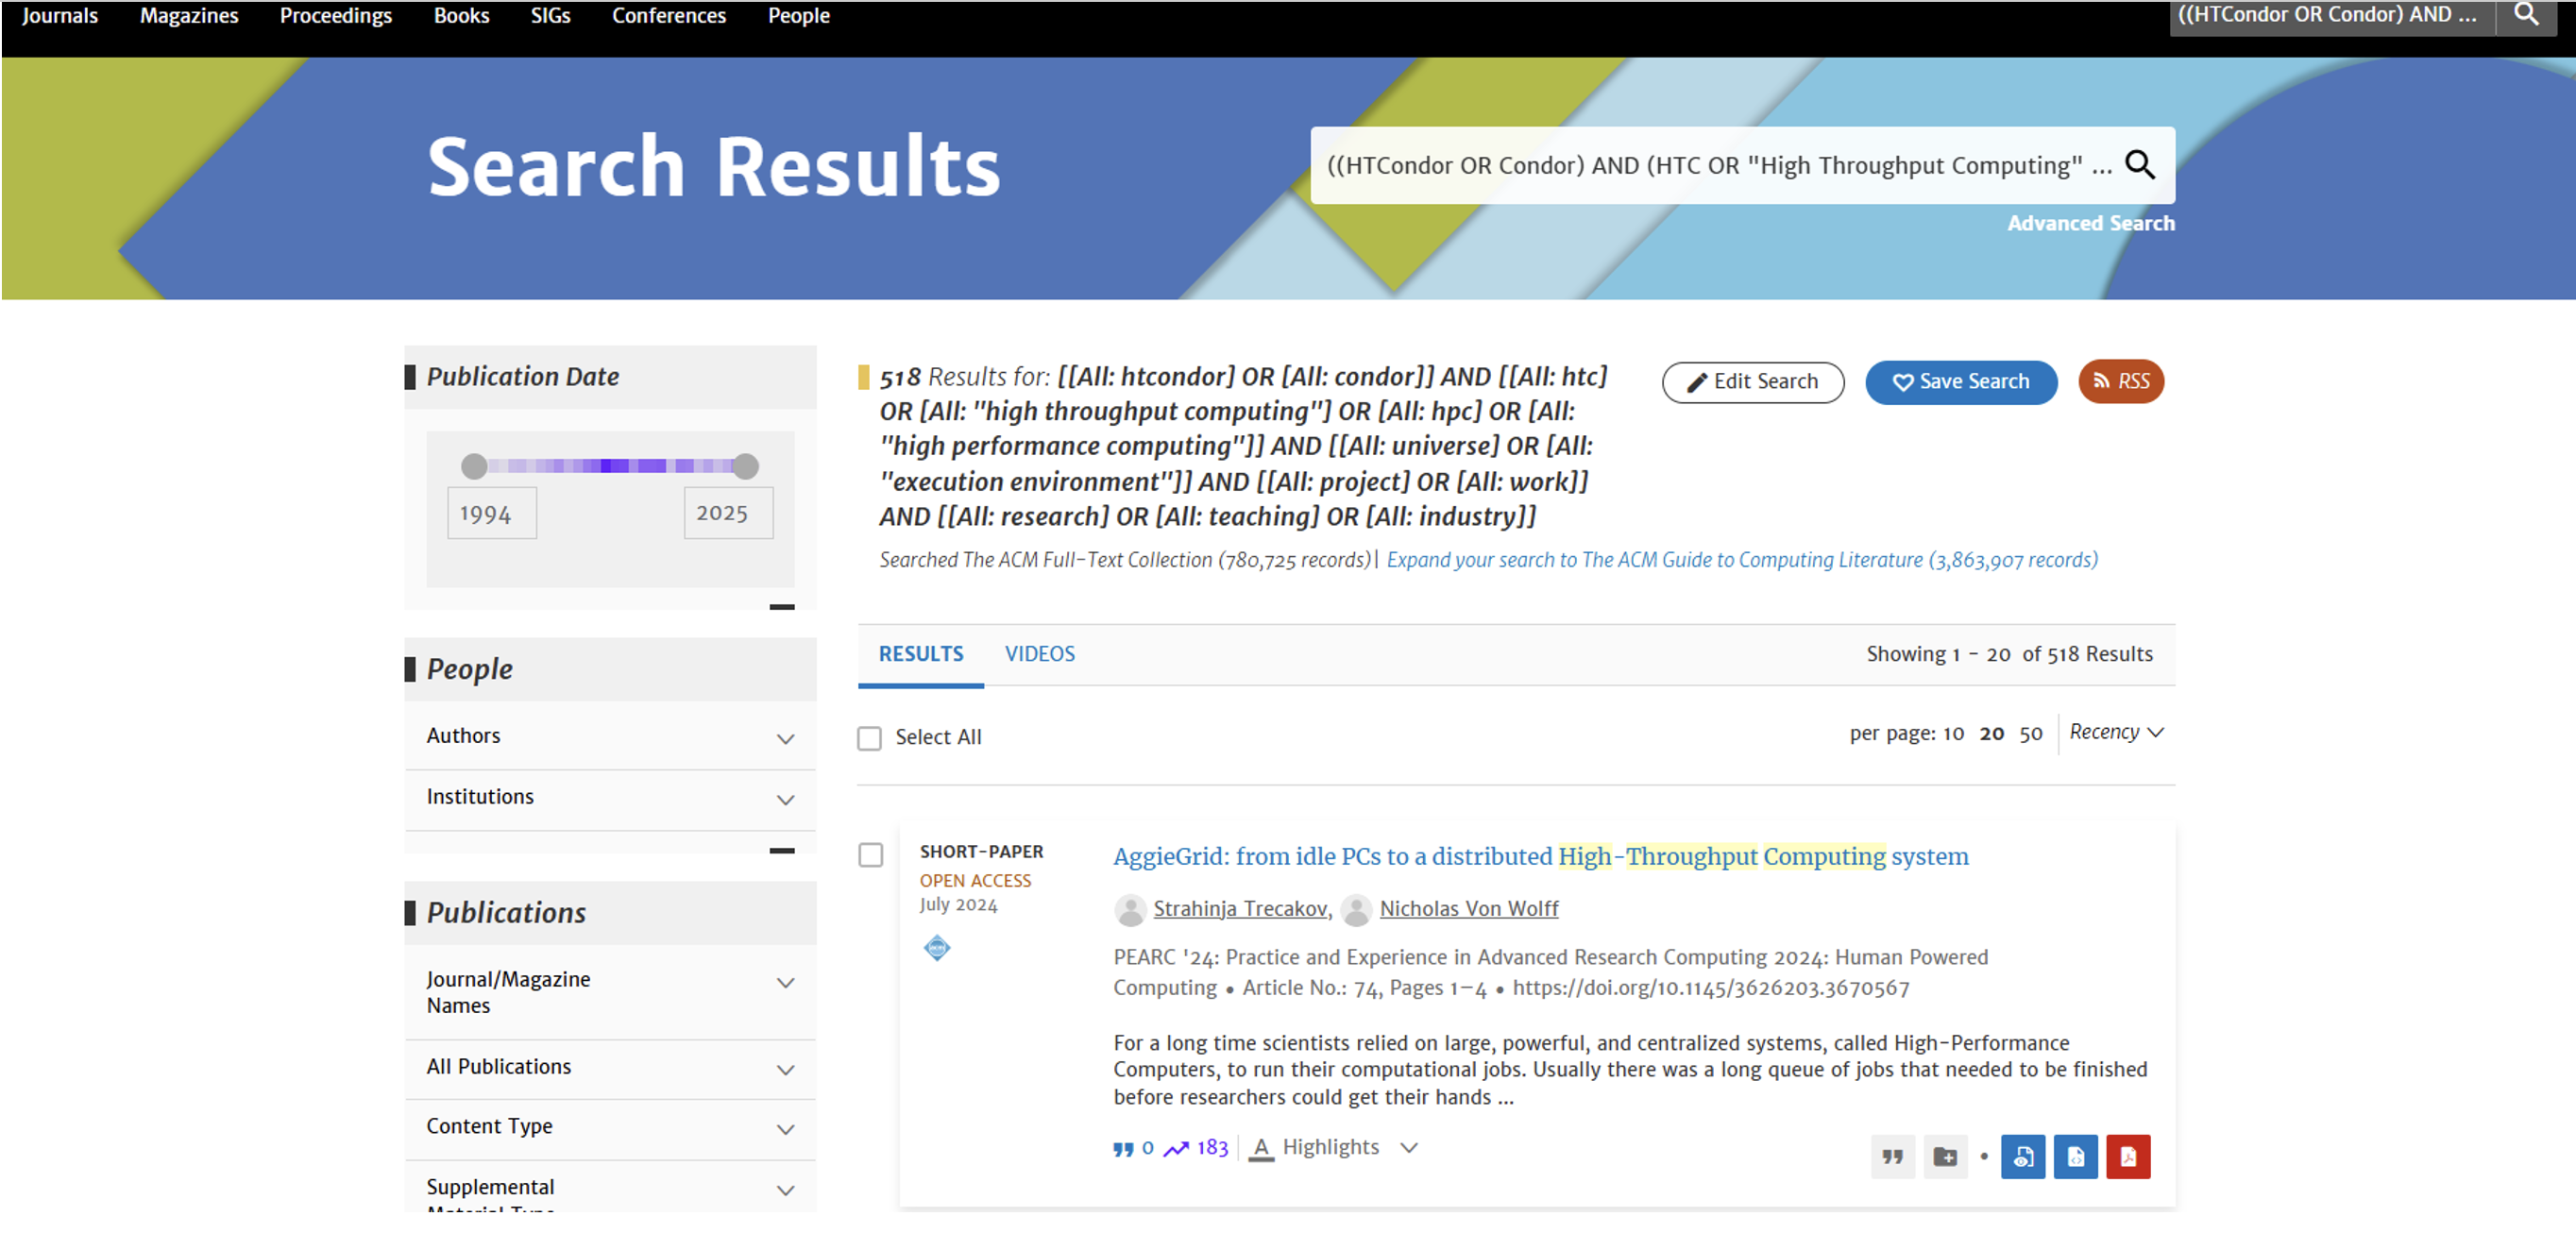
\includegraphics[width=\textwidth,keepaspectratio]{apendices/bases-datos/sin-exclusion/acm.png}
	\caption{Búsqueda de artículos de educación en ACM sin criterios de inclusión/exclusión \\
		Fecha de acceso: 12/03/25 9:13 pm
	}\label{fig:busqueda-acm-no-exclusion}
\end{figure}

\FloatBarrier

\begin{figure}[H]
	\centering
	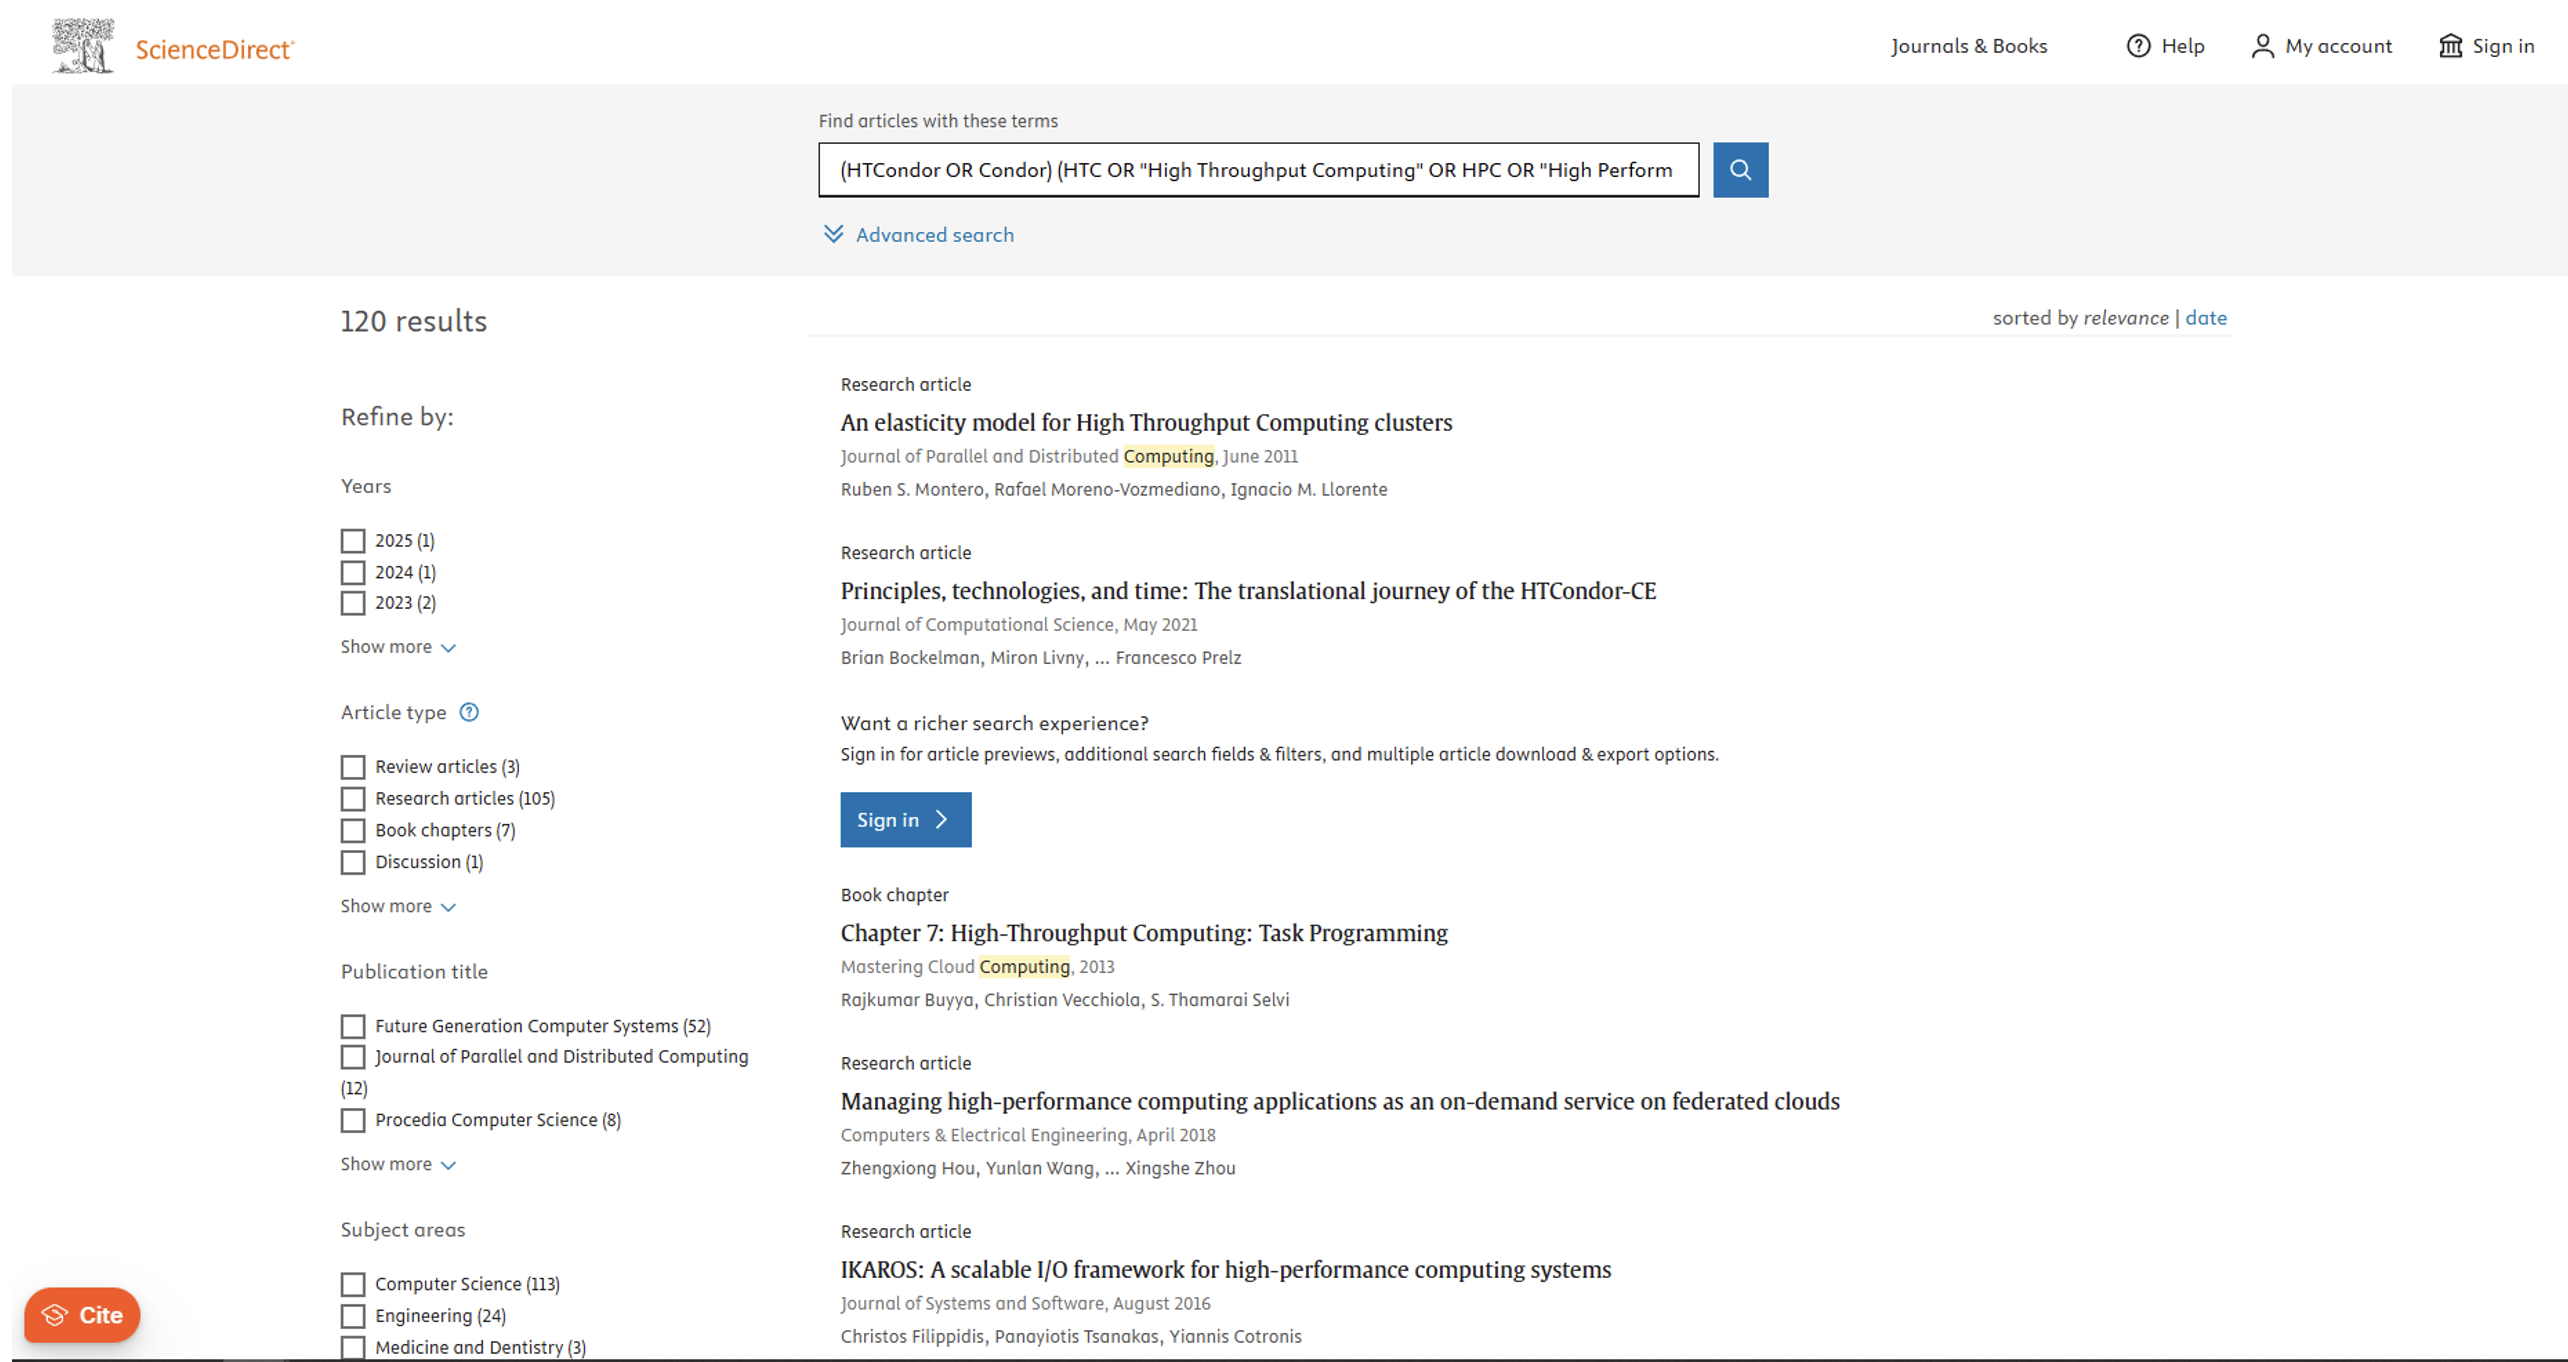
\includegraphics[width=\textwidth,keepaspectratio]{apendices/bases-datos/sin-exclusion/science-direct.png}
	\caption{Búsqueda de artículos de investigación en ACM sin criterios de inclusión/exclusión \\
		Fecha de acceso: 12/03/25 8:23 pm
	}\label{fig:busqueda-science-direct-no-exclusion}
\end{figure}

\begin{figure}[H]
	\centering
	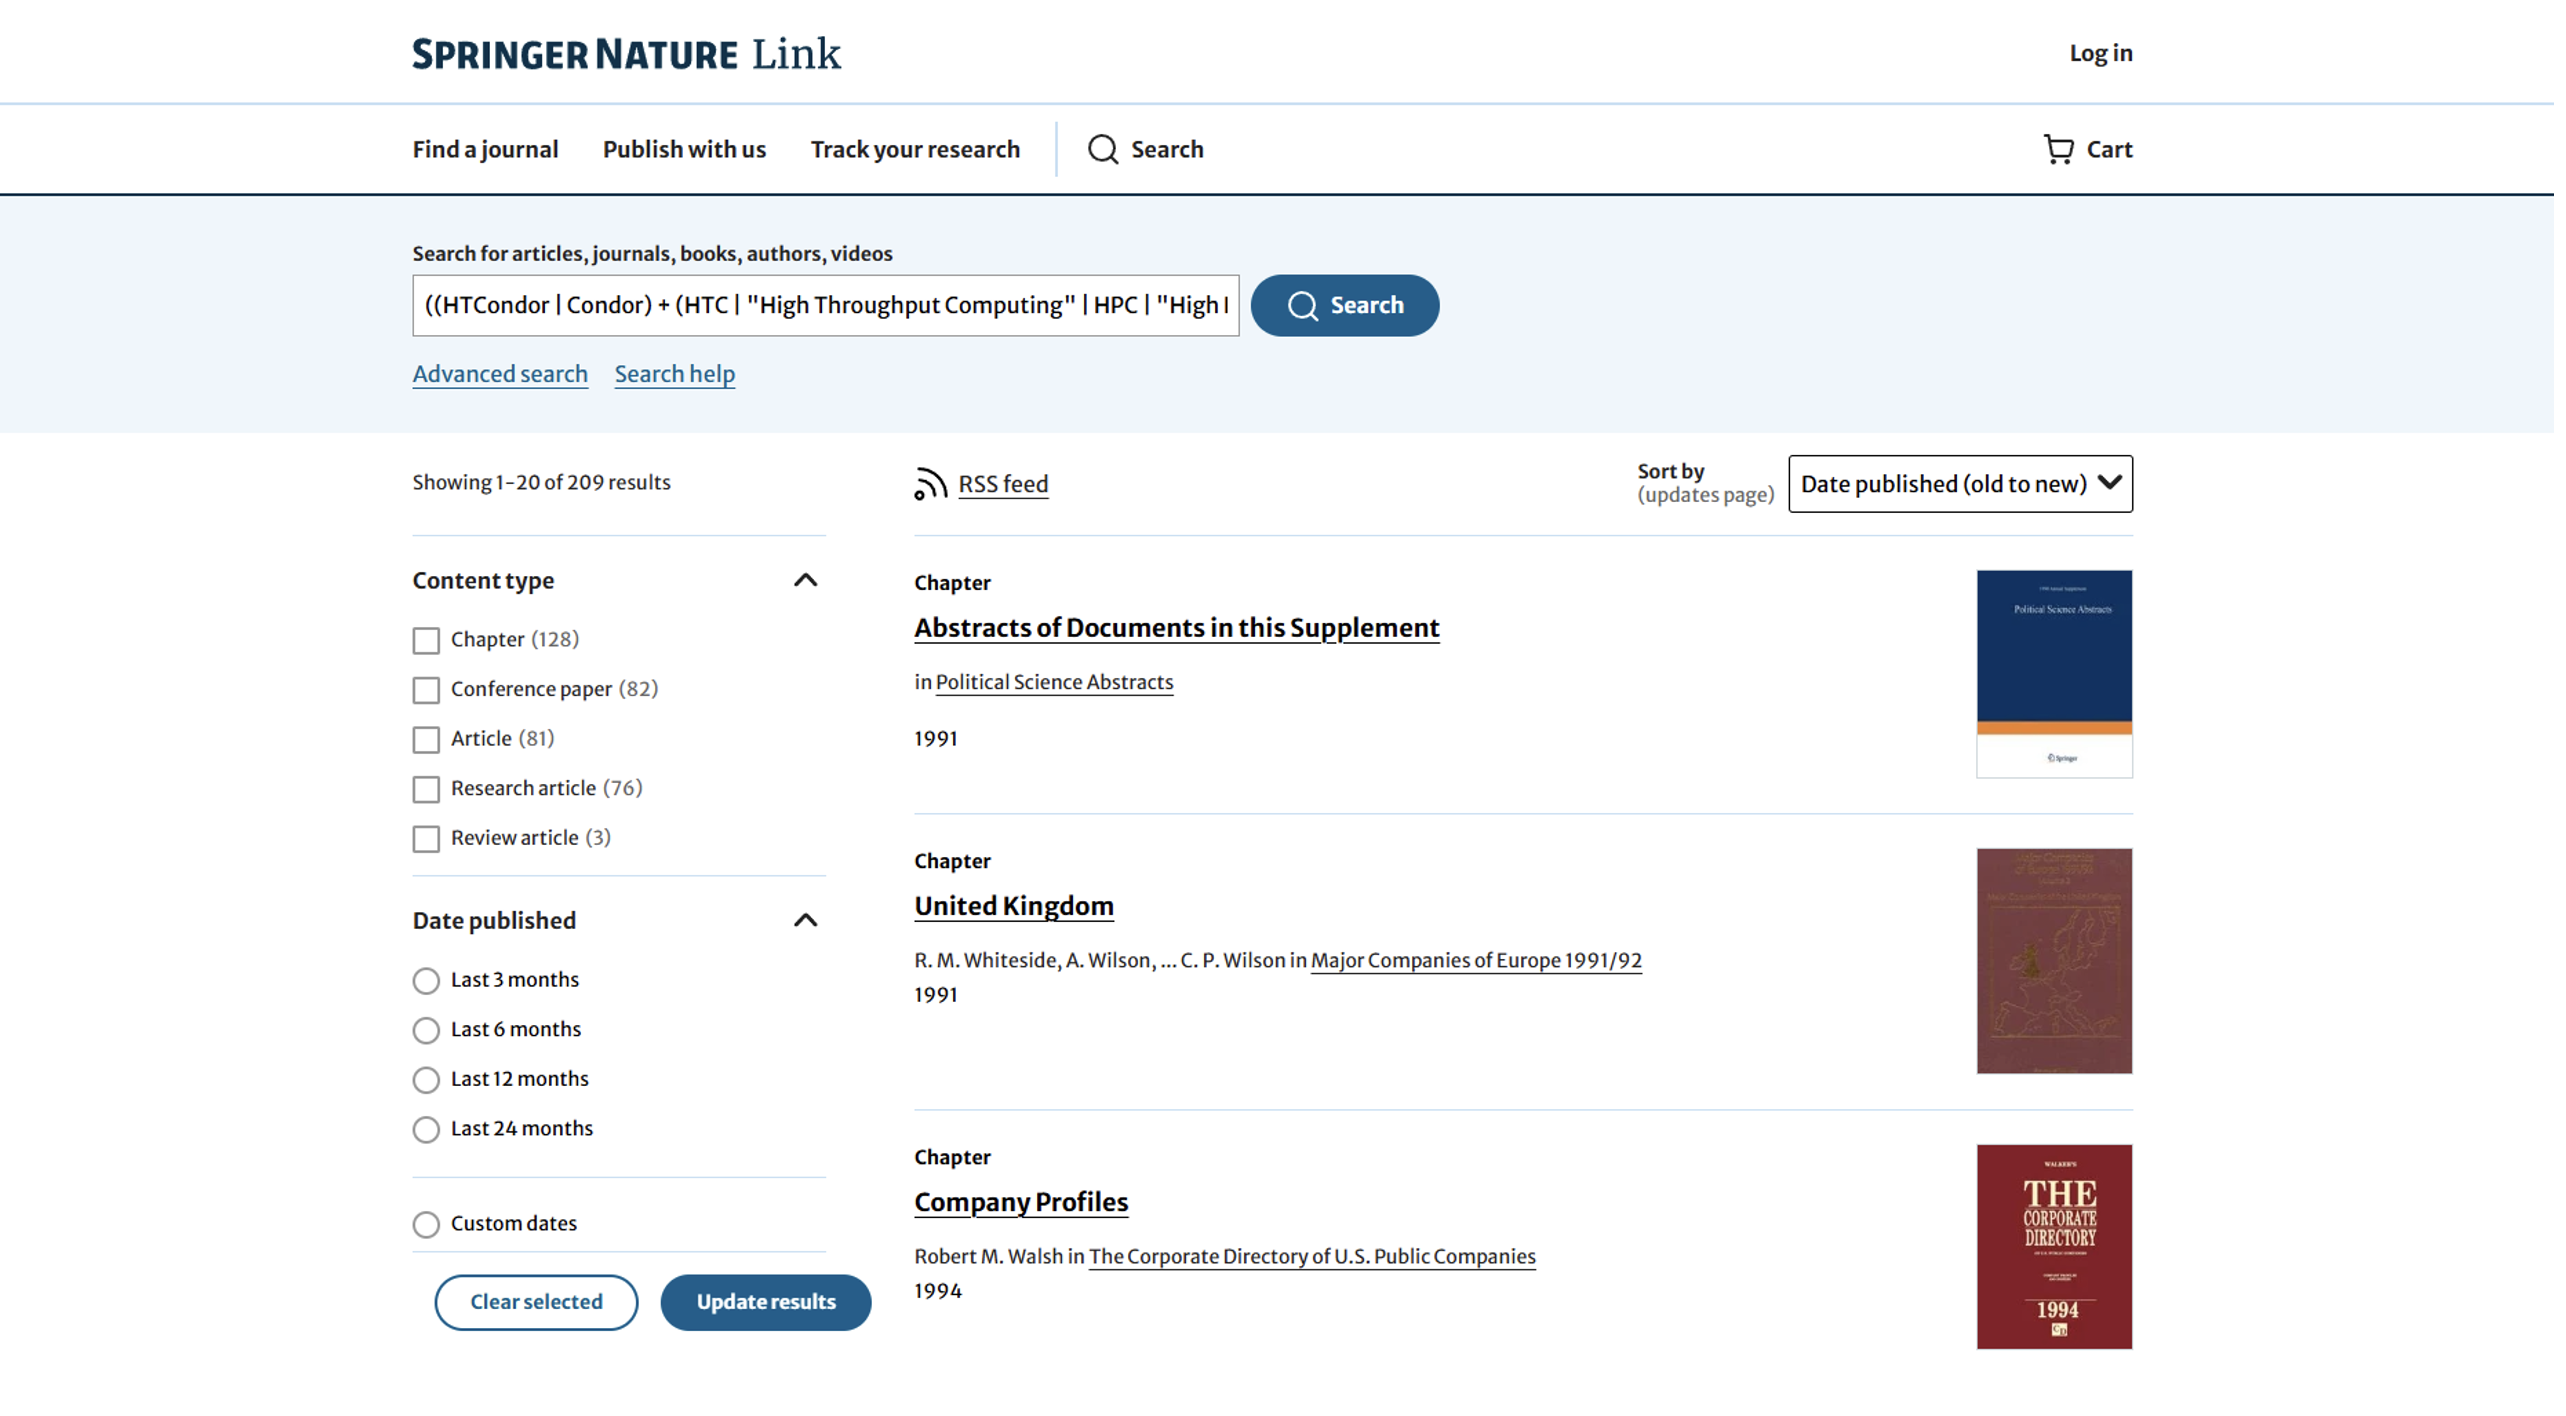
\includegraphics[width=\textwidth,keepaspectratio]{apendices/bases-datos/sin-exclusion/springer.png}
	\caption{Búsqueda de artículos de investigación en ACM sin criterios de inclusión/exclusión \\
		Fecha de acceso: 12/03/25 8:23 pm
	}\label{fig:busqueda-springer-no-exclusion}
\end{figure}


%########## Fin Imagenes %###################


\section{Búsqueda de artículos con criterios de inclusión/exclusión}\label{sec:busqueda-con-criterios}

\begin{figure}[H]
	\centering
	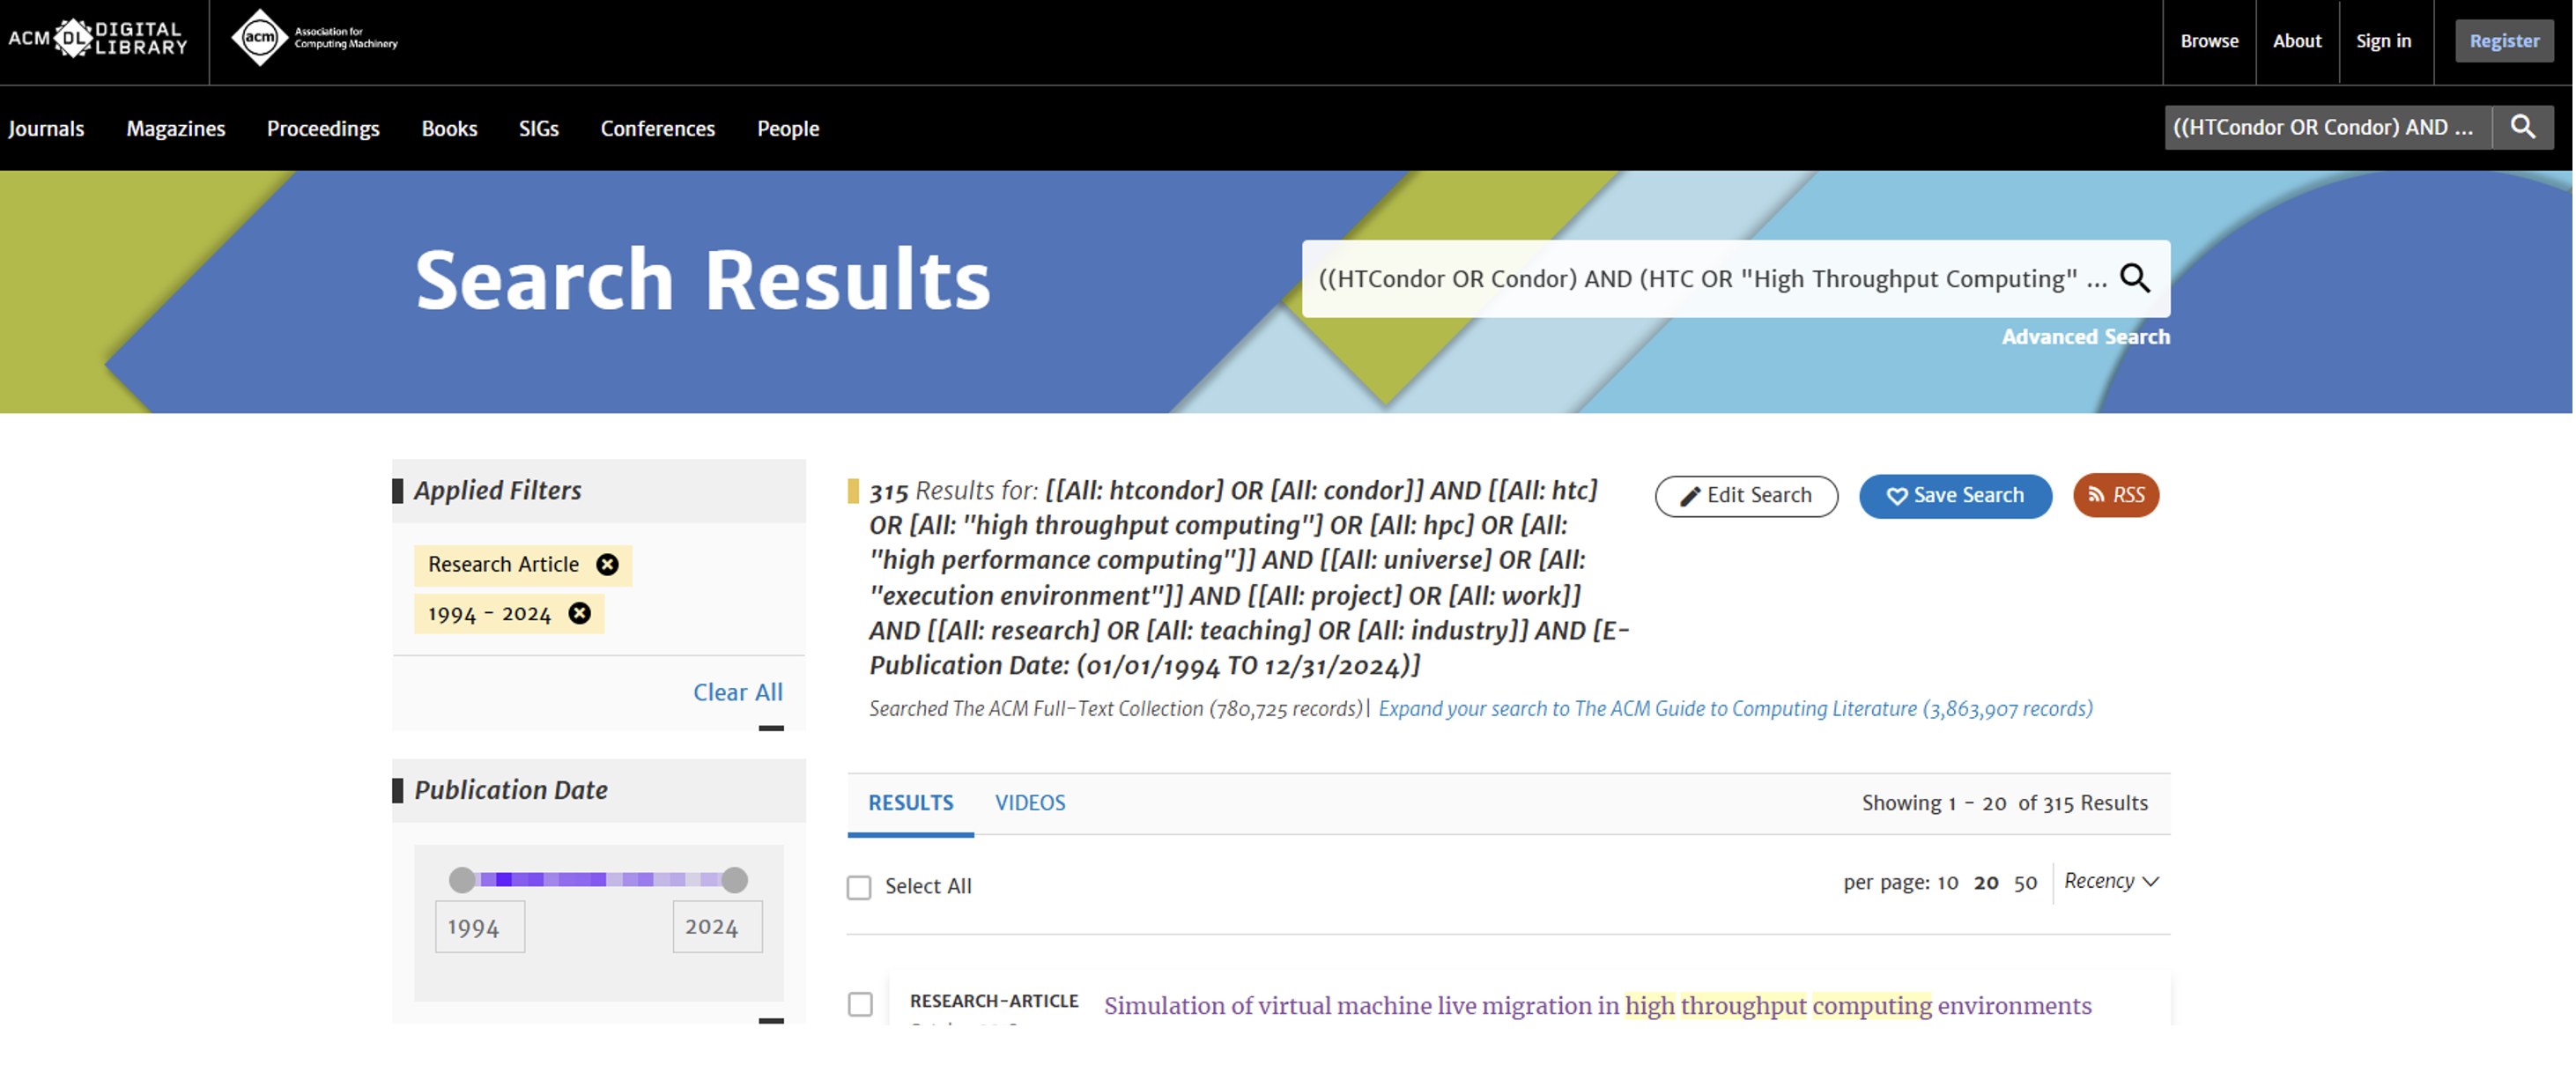
\includegraphics[width=\textwidth,keepaspectratio]{apendices/bases-datos/con-exclusion/acm.png}
	\caption{Búsqueda de artículos de educación en ACM sin criterios de inclusión/exclusión \\
		Fecha de acceso: 12/03/25 9:13 pm
	}\label{fig:busqueda-acm-con-exclusion}
\end{figure}

\FloatBarrier

\begin{figure}[H]
	\centering
	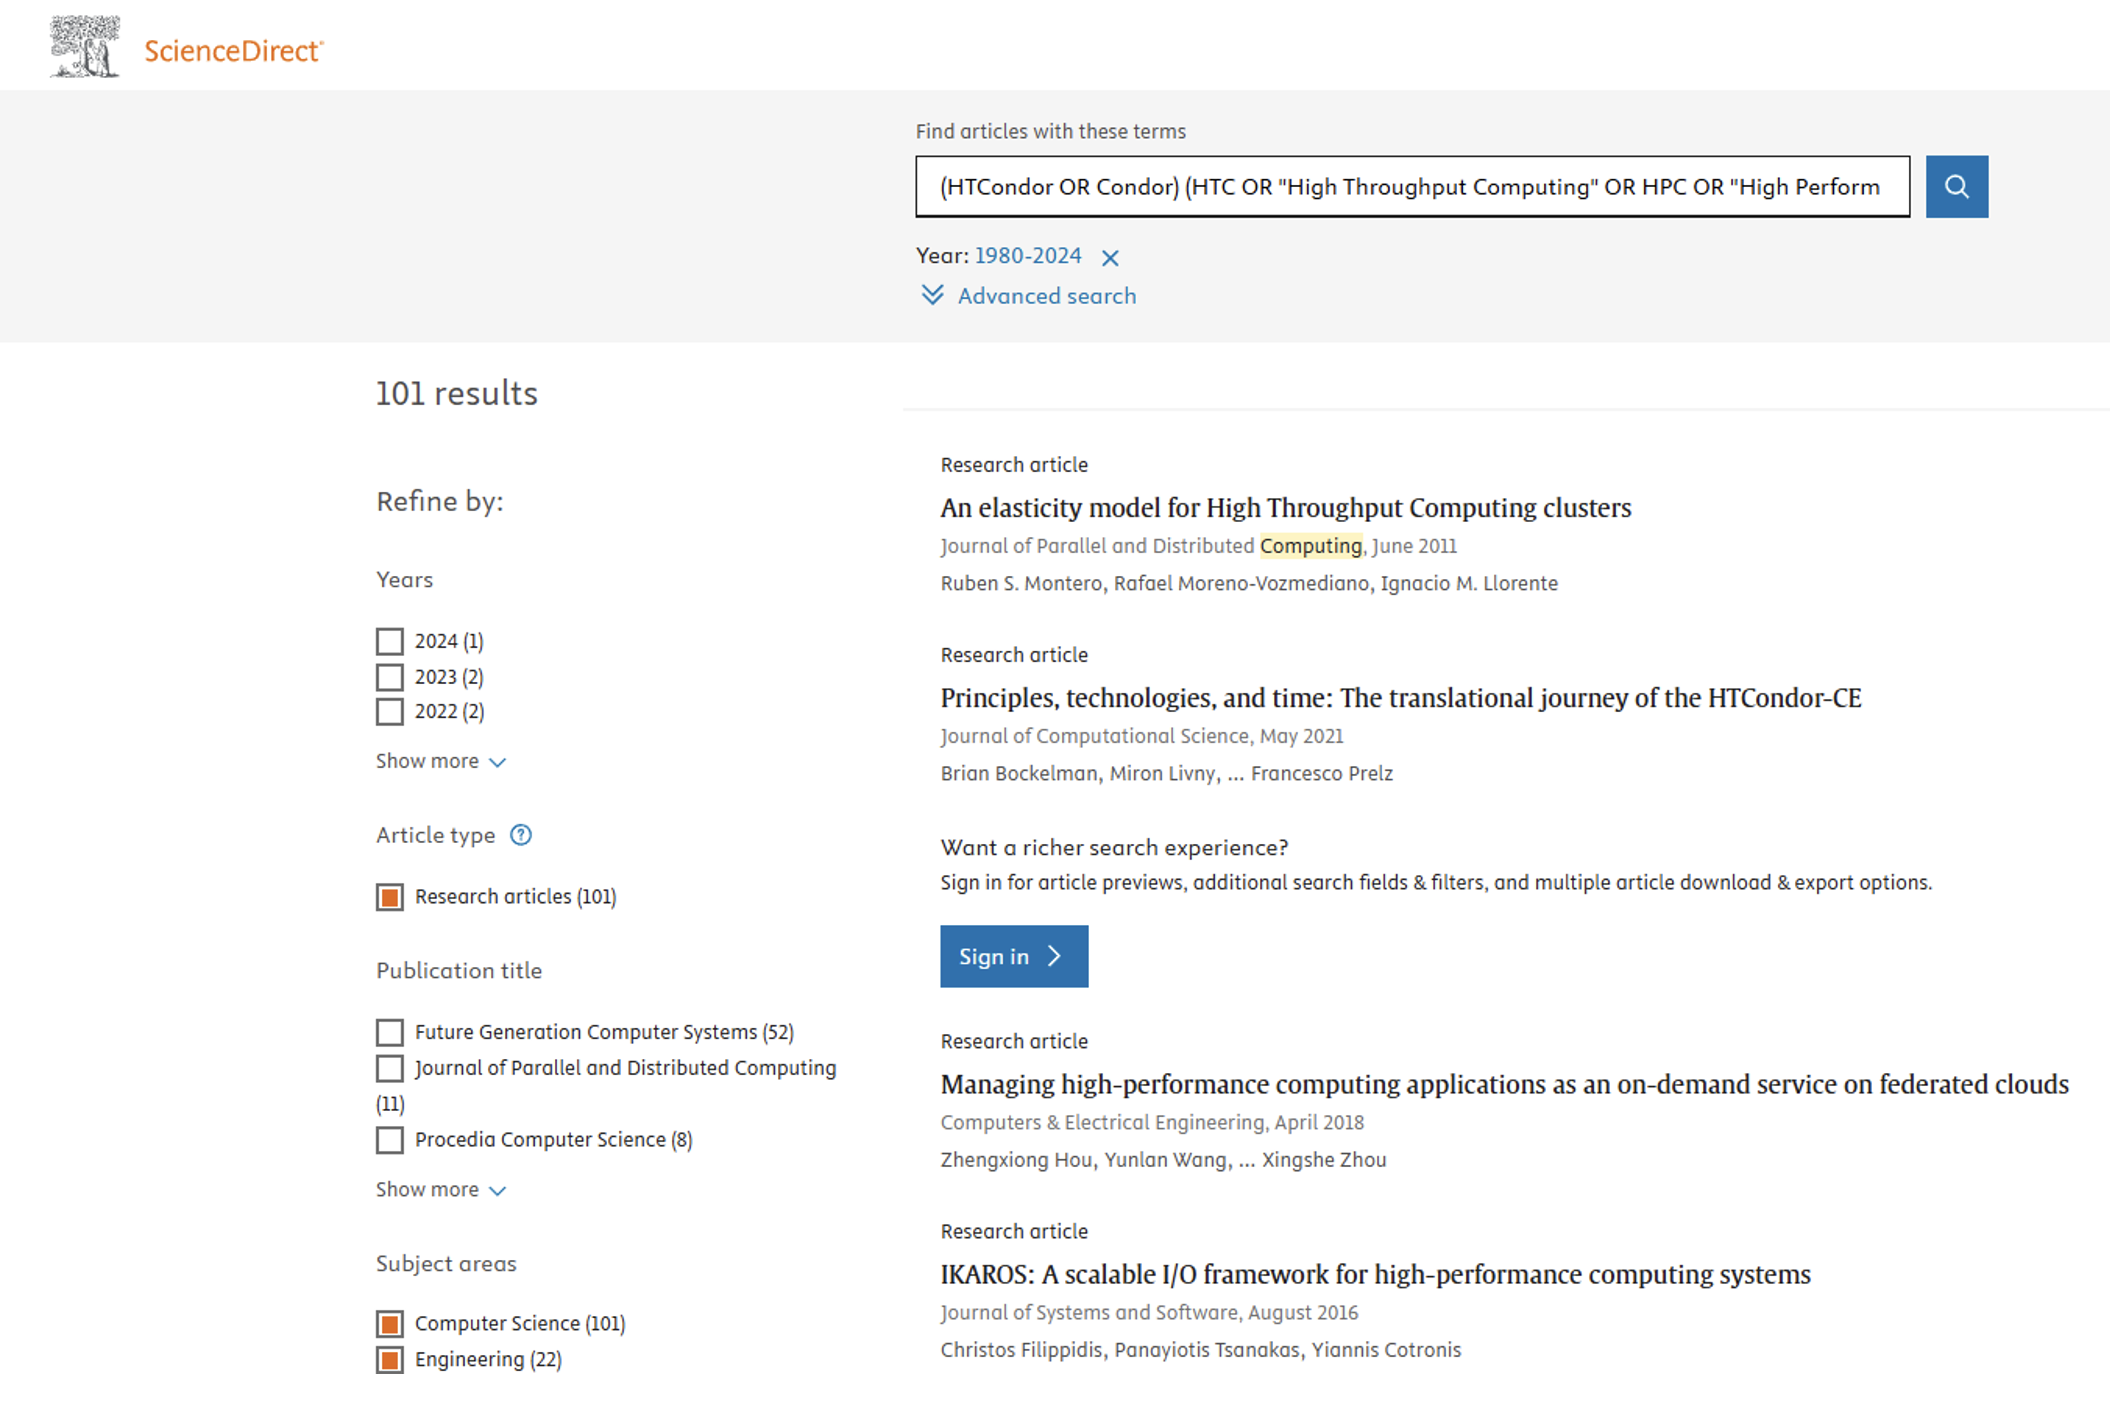
\includegraphics[width=\textwidth,keepaspectratio]{apendices/bases-datos/con-exclusion/science-direct.png}
	\caption{Búsqueda de artículos de investigación en ACM sin criterios de inclusión/exclusión \\
		Fecha de acceso: 12/03/25 8:23 pm
	}\label{fig:busqueda-science-direct-con-exclusion}
\end{figure}

\begin{figure}[H]
	\centering
	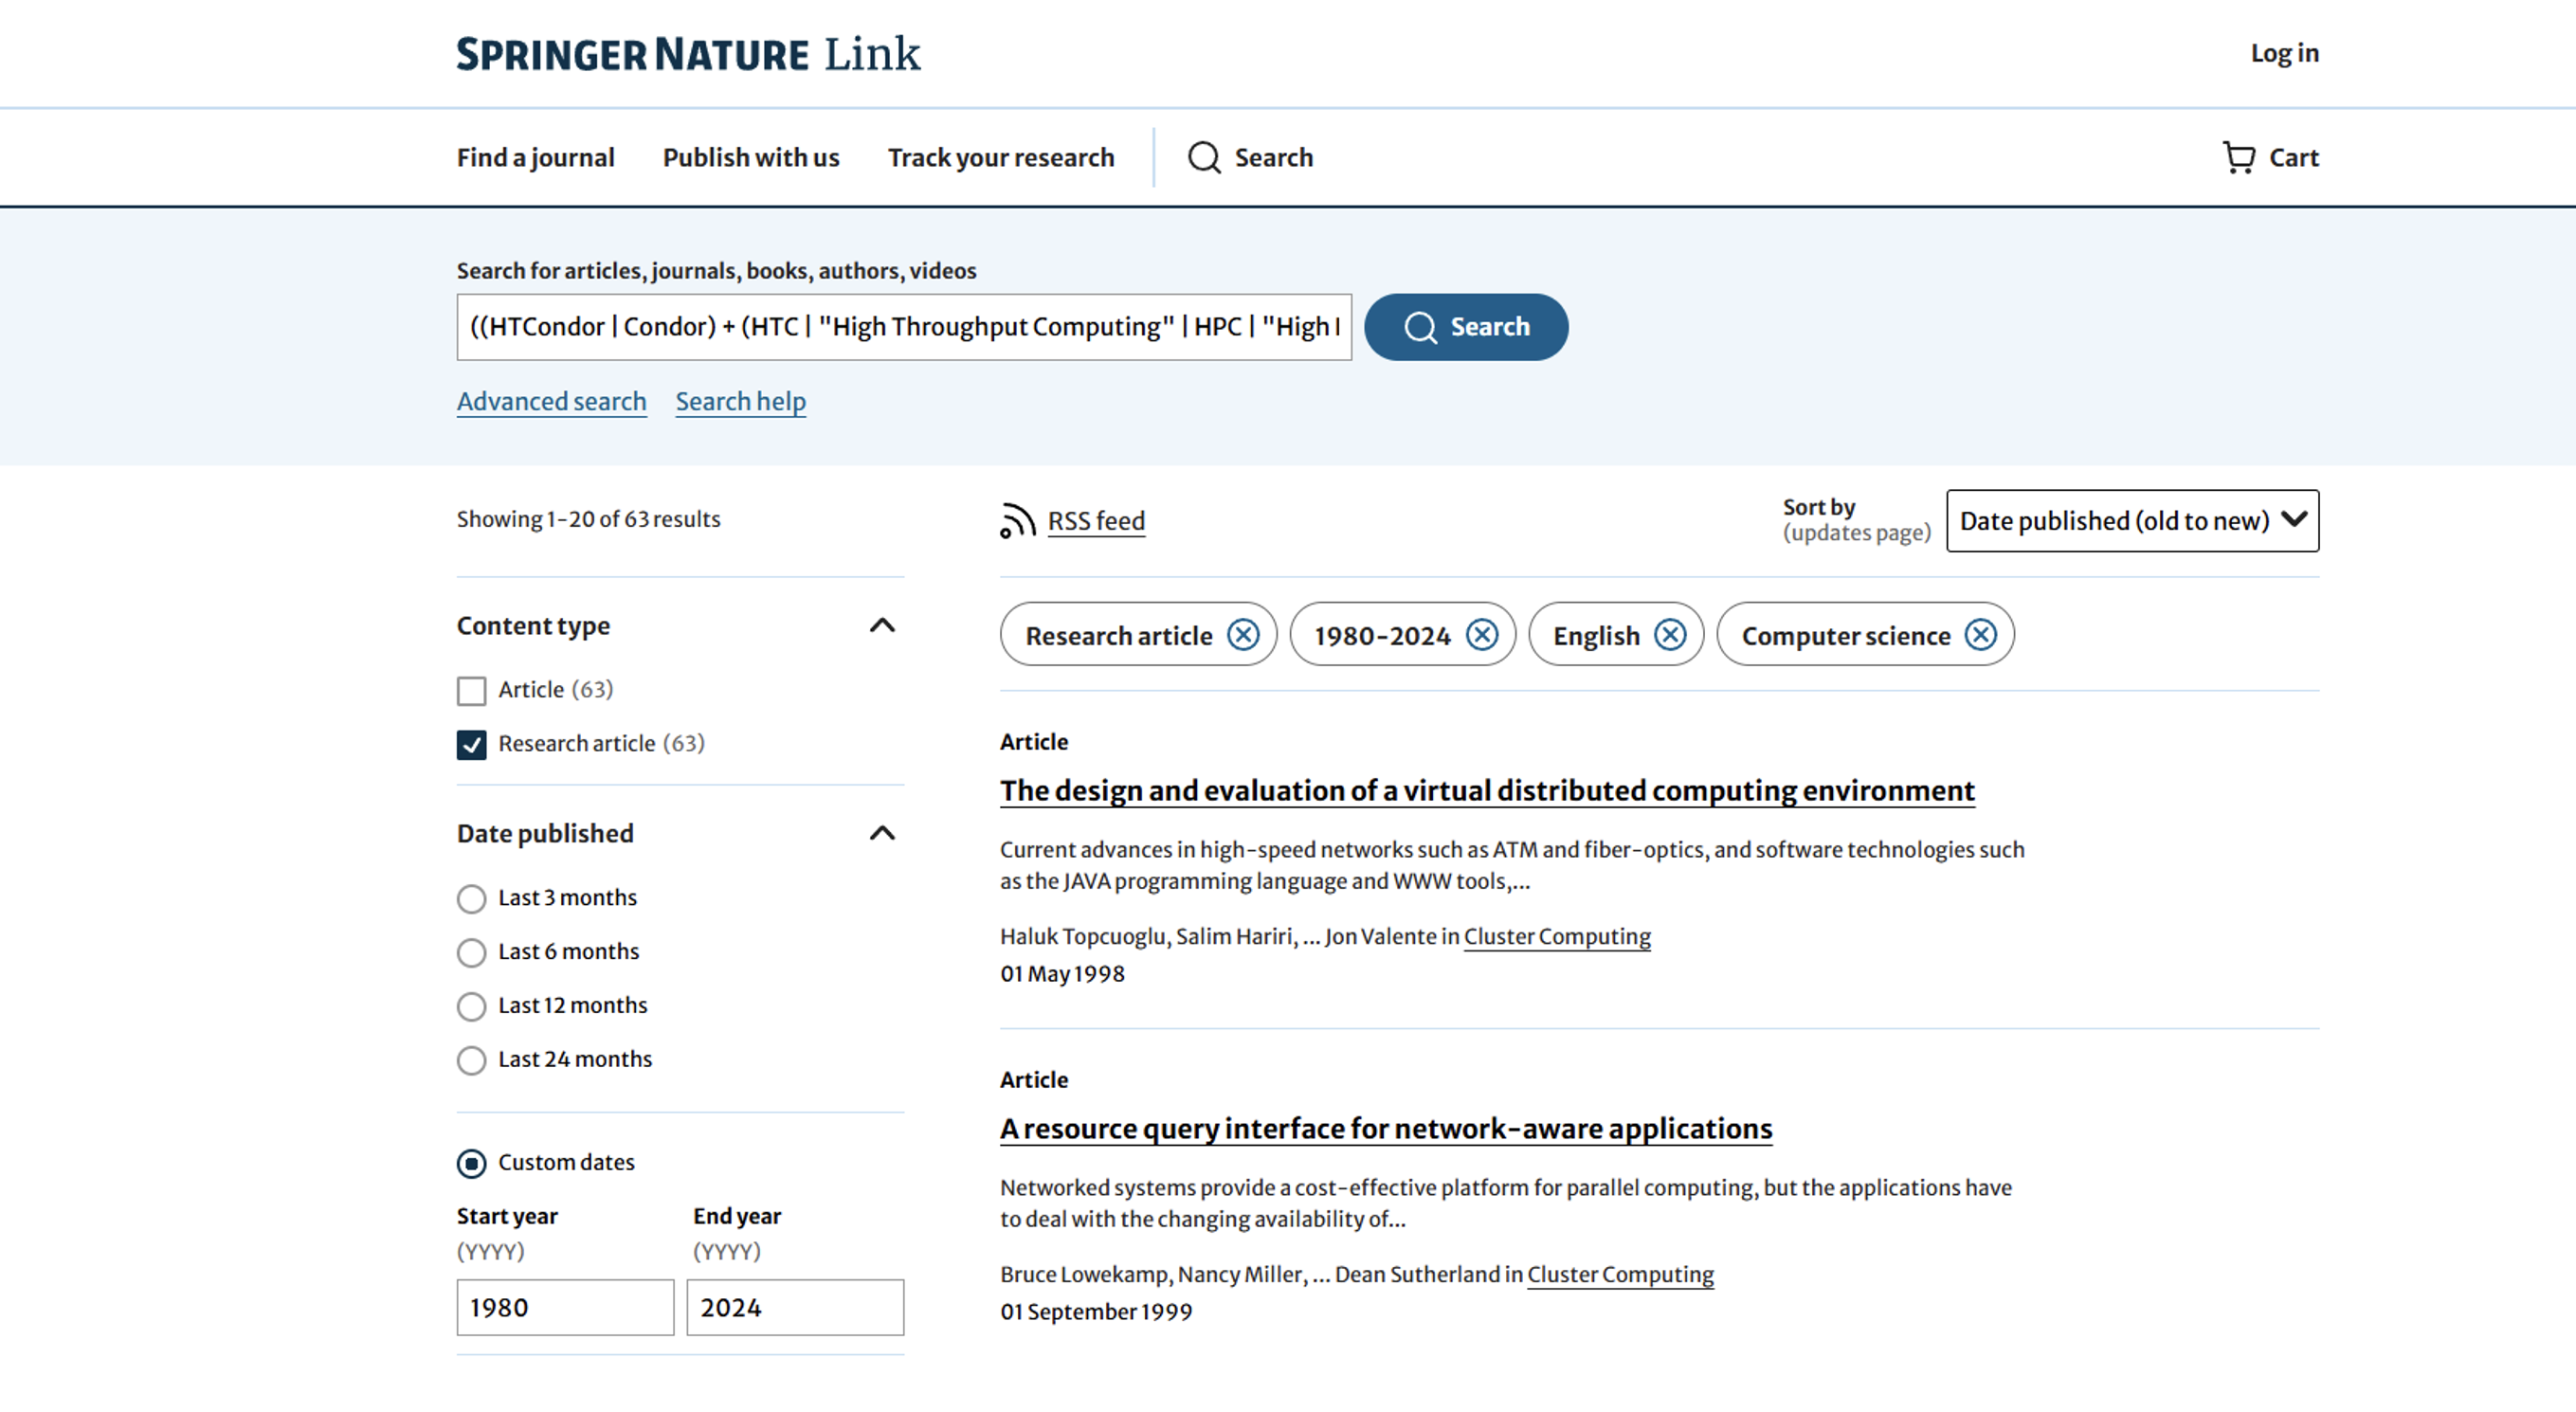
\includegraphics[width=\textwidth,keepaspectratio]{apendices/bases-datos/con-exclusion/springer.png}
	\caption{Búsqueda de artículos de investigación en ACM sin criterios de inclusión/exclusión \\
		Fecha de acceso: 12/03/25 8:23 pm
	}\label{fig:busqueda-springer-con-exclusion}
\end{figure}

\newpage



% CHAPTER Implementación del univeso Parallel
\phantomsection

% Increment the chapter counter so \thechapter shows the correct number
% and make it referenceable with \ref
\refstepcounter{chapter}

% Manually add this appendix to the Table of Contents
\addcontentsline{toc}{chapter}{Apéndice \thechapter: Implementación del clúster virtualizado HTCondor}

% Add vertical space above the title (mimics standard chapter spacing)
\vspace{40pt}

% Display the actual chapter title (centered, large, bold)
{\centering \normalfont\huge\bfseries Apéndice~\thechapter: Implementación del clúster virtualizado HTCondor~\par}

% Add spacing between title and horizontal rule
\vspace{10pt}

% Draw a horizontal line across the page for visual separation
{\centering \rule{\textwidth}{0.4pt} \par}

% Add vertical space between title section and content
\vspace{40pt}

% Set the running headers for left and right pages
\markboth{Apéndice \thechapter: Implementación del clúster virtualizado HTCondor}{Apéndice \thechapter: Implementación del clúster virtualizado HTCondor}


\FloatBarrier\subsection{Instalación en un entorno virtualizado}

El clúster de computación distribuida de HTCondor actualmente soporta la versión \texttt{8.4.11}. A continuación se muestra la salida de uno de los nodos Raspberry-Pi, los cuales tienen una instalación heterogénea:

% HTCondor version output
\begin{minted}[
    frame=lines,
    framesep=2mm,
    baselinestretch=1.2,
    bgcolor=lightgray!10,
    fontsize=\footnotesize,
]{bash}
condor_version
$CondorVersion: 8.4.11 Feb 06 2017 BuildID: Debian-8.4.11~dfsg.1-1 Debian-8.4.11~dfsg.1-1
$$CondorPlatform: ARMV7L-Raspbian_ $
\end{minted}


Si bien esta versión es compatible con el \textbf{universo parallel}, la limitada documentación disponible para la version \texttt{8.4.11} en particular representó un obstáculo para implementar algoritmos que utilizaran OpenMPI. Por esta razón, y siguiendo la recomendación del asesor de este proyecto, se decidió implementar dicho universo en una infraestructura virtualizada.

\FloatBarrier\subsubsection{Infraestrutura virtualizada}

El primer paso hacia la implementación de la nueva infraestructura HTCondor fue desplegar máquinas virtuales en la infraestructura del \GRID. Para ello se utilizó un servidor dedicado que ejecuta el hipervisor \cite{xcpng_intro}, en el cual se configuraron 5 máquinas virtuales con el sistema operativo~\texttt{AlmaLinux 9.6 (Sage Margay) x86\_64}. Las máquinas pueden verse, mediante la interfaz Xen-Orchestra en la figura \ref{fig:xen-vms}. Esta configuración difiere significativamente de la arquitectura armv7l de 32 bits que utiliza el clúster de Raspberry Pi actual. La elección de este sistema operativo no fue trivial, se fundamentó en varios criterios: según la documentación oficial, AlmaLinux es uno de los sistemas operativos oficialmente soportados por HTCondor~\cite{HTCondor_install}, además de haber sido implementado exitosamente por instituciones como el CERN \citep{Bunsic2025}.

\begin{figure}
	\centering
	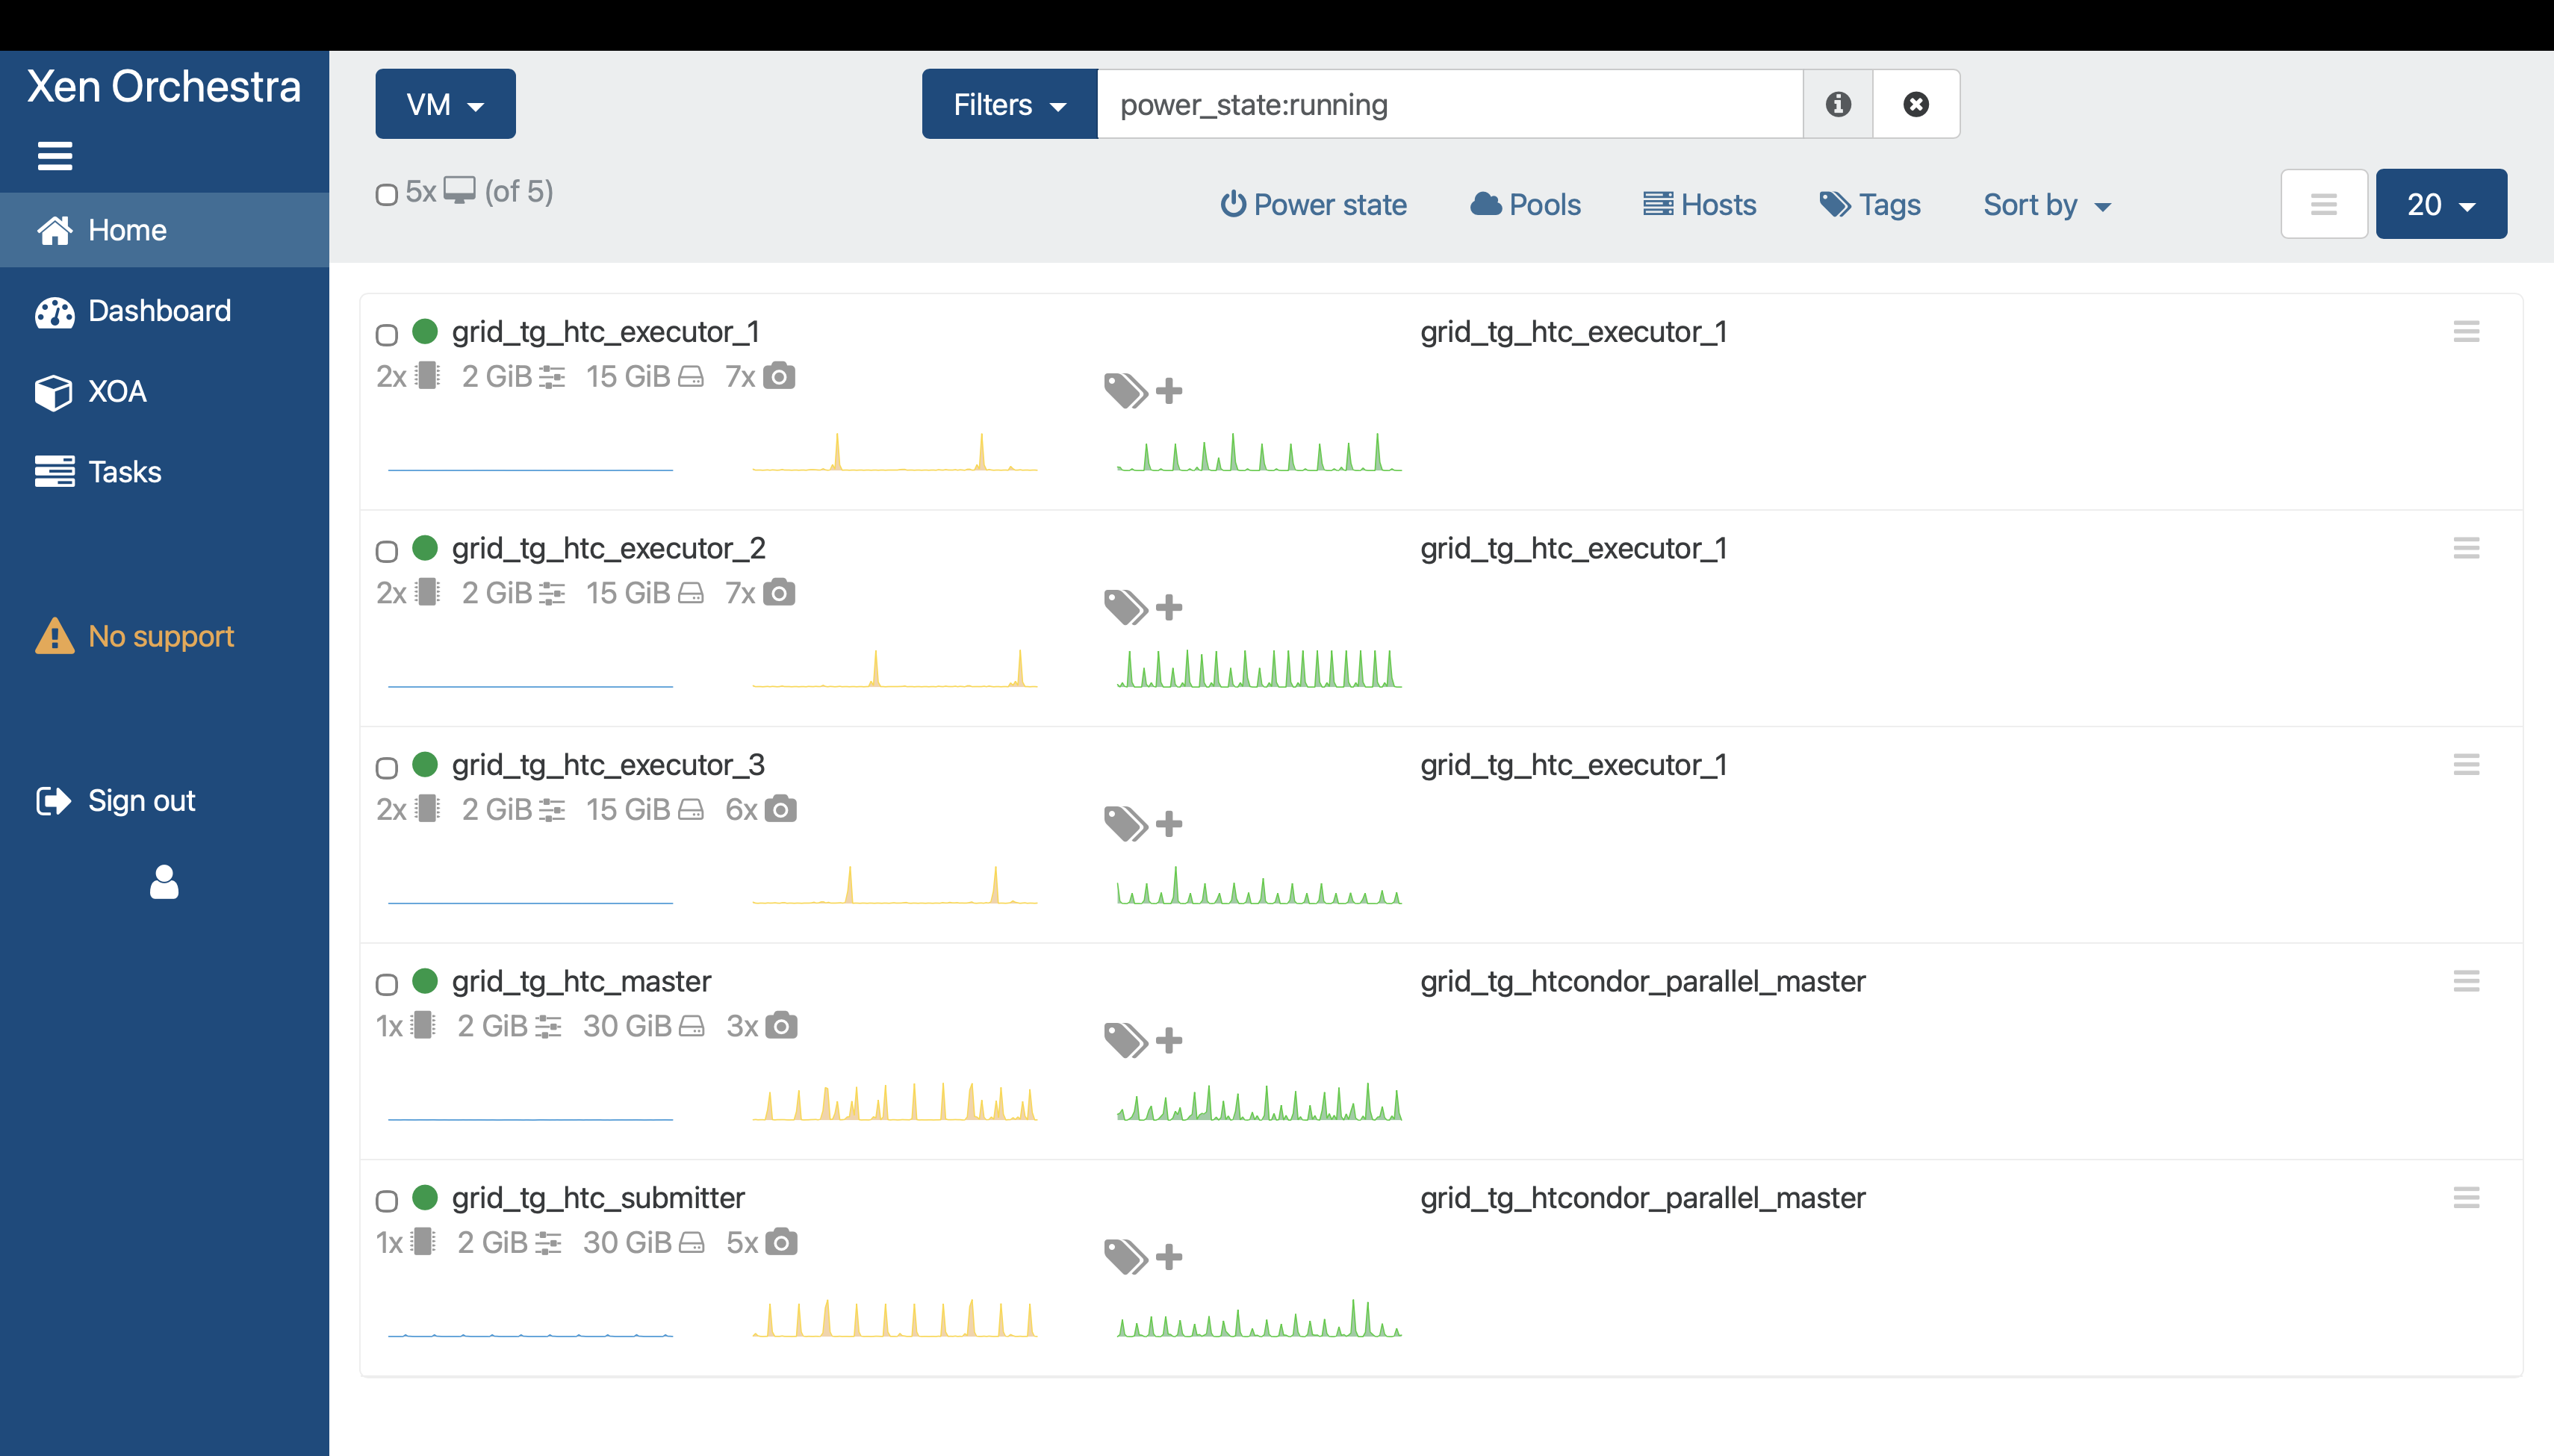
\includegraphics[scale=0.25]{apendices/infra-virtual/xen-vms.png}
	\caption{Vista de las máquinas virtuales para la nueva infraestructura HTCondor virtualizada de \GRID}
	\label{fig:xen-vms}
\end{figure}

A cada máquina se le asignó, al momento de instalación, una dirección IP dentro de la red \texttt{172.30.28.0/24} como se muestra en la Tabla~\ref{tab:nodos-htcondor}:

\begin{table}[H]
	\centering
	\renewcommand{\arraystretch}{1.2} % Espaciado reducido
	\fontsize{9pt}{10pt}\selectfont % Tamaño de fuente 9pt
	\begin{tabular}{|p{3cm}|p{3cm}|p{4.5cm}|p{2.5cm}|}  % Total: 14cm (incluyendo bordes)
		\hline
		\textbf{Rol del nodo} & \textbf{Dirección IP} & \textbf{Nombre de usuario} & \textbf{Usuario} \\ \hline
		Grid Manager          & 172.30.28.29          & gridmanager                & alma             \\ \hline
		Master                & 172.30.28.30          & master                     & alma             \\ \hline
		Submit                & 172.30.28.31          & submit                     & alma             \\ \hline
		Ejecutor 1            & 172.30.28.32          & exec01                     & alma             \\ \hline
		Ejecutor 2            & 172.30.28.33          & exec02                     & alma             \\ \hline
		Ejecutor 3            & 172.30.28.34          & exec03                     & alma             \\ \hline
	\end{tabular}
	\caption{Configuración de nodos del clúster HTCondor virtualizado}
	\label{tab:nodos-htcondor}
\end{table}


\FloatBarrier\subsubsection{Instalación de HTCondor}

Para la instalación de HTCondor se diseño el siguiente script, el cual emplea otro script que puede encontrarse en la documentación oficial \cite{HTCondor-linux-install}.



% HTCondor Install script
\begin{minted}[
    frame=lines,
    framesep=2mm,
    baselinestretch=1.2,
    bgcolor=lightgray!10,
    fontsize=\footnotesize,
]{bash}
#!/bin/bash

# Script de instalación de HTCondor para Alma Linux 9.6
# Uso: ./install-condor.sh <tipo_nodo> <hostname_master> <contraseña>
# Tipos de nodo: master, submit, worker

if [ "$#" -ne 3 ]; then
    echo "Uso: $0 <tipo_nodo> <hostname_master> <contraseña>"
    echo "Tipos de nodo: master, submit, worker"
    echo "Ejemplo: $0 master master.example.com micontraseña"
    exit 1
fi

NODE_TYPE=$1 #Tipo de nodo, hay tres opciones: {'master', 'submit' y 'worker;}
MASTER_FQN=$2 # Fully Qualified Name del nodo maestro.
PASSWORD=$3 #Deberá ser igual para todos los nodos de manera que puedan comunicarse entre sí

sudo dnf update -y

case $NODE_TYPE in
    master)
        echo "Instalando nodo MASTER..."
        curl -fsSL https://get.htcondor.org | sudo /bin/bash -s -- --no-dry-run --cm $MASTER_FQN --password $PASSWORD --channel lts
        ;;
    submit)
        echo "Instalando nodo SUBMIT (access point)..."
        curl -fsSL https://get.htcondor.org | sudo /bin/bash -s -- --no-dry-run --ap $MASTER_FQN --password $PASSWORD --channel lts
        ;;
    worker)
        echo "Instalando nodo WORKER (execution point)..."
        curl -fsSL https://get.htcondor.org | sudo /bin/bash -s -- --no-dry-run --ep $MASTER_FQN --password $PASSWORD --channel lts
        ;;
    *)
        echo "Error: Tipo de nodo inválido. Use: master, submit o worker"
        exit 1
        ;;
esac

echo "Instalación completada exitosamente!"
\end{minted}


Aparte del script anterior, también se creó una guía en formato .md la cual puede ser encontrada en el siguiente \href{https://github.com/Parritap/HTcondor/blob/master/alma-linux-cluster/README-ES.md}{https://github.com/Parritap/HTcondor/blob/master/alma-linux-cluster/README-ES.md}.



Para HTcondor es muy importante que los nodos puedan comunicarse entre sí, para lograr esto, se editaron los archivos \texttt{/etc/hosts} en cada uno de los nodos. Dicha edición puede verse en a continuación:

% HTCondor Install script
\begin{minted}[
    frame=lines,
    framesep=2mm,
    baselinestretch=1.2,
    bgcolor=lightgray!10,
    fontsize=\footnotesize,
]{bash}
#Parallel config
172.30.28.30 master
172.30.28.31 submit
172.30.28.32 exec01
172.30.28.33 exec02
172.30.28.34 exec03
172.30.28.35 exec04
\end{minted}

Después de dicha configuración podremos ejecutar el comando \texttt{condor\_status} y ver lo siguiente impreso en consola:

\begin{minted}[
    frame=lines,
    framesep=2mm,
    baselinestretch=1.2,
    bgcolor=lightgray!10,
    fontsize=\footnotesize,
]{bash}
Name         OpSys      Arch   State     Activity LoadAv Mem   ActvtyTime

slot1@exec01 LINUX      X86_64 Unclaimed Idle      0.000 1763  6+02:39:58
slot1@exec02 LINUX      X86_64 Unclaimed Idle      0.000 1763  6+02:34:51
slot1@exec03 LINUX      X86_64 Unclaimed Idle      0.000 1763  6+02:34:43

               Total Owner Claimed Unclaimed Matched Preempting  Drain Backfill BkIdle

  X86_64/LINUX     3     0       0         3       0          0      0        0      0

         Total     3     0       0         3       0          0      0        0      0

\end{minted}

%!TODO
\FloatBarrier\subsection{Instalación de un implementación \MPI}

Para permitir la comunicación entre trabajos distribuidos fuertemente acoplados en un pool HTCondor, es necesario implementar una tecnología basada en el estándar~\MPI. En este contexto, se seleccionó OpenMPI debido a que, según la documentación oficial de HTCondor \cite{HTCondor_Parallel}, esta implementación particular del estándar MPI cuenta con soporte nativo, lo que facilita su integración con el sistema de gestión de trabajos. El script de instalación de OpenMPI para el sistema operativo Alma Linux se presenta a continuación:

% HTCondor Install script
\begin{minted}[
    frame=lines,
    framesep=2mm,
    baselinestretch=1.2,
    bgcolor=lightgray!10,
    fontsize=\footnotesize,
]{bash}
sudo dnf update -y
sudo dnf install openmpi openmpi-devel -y

echo "module load mpi/openmpi-x86_64" >> ~/.bashrc
source ~/.bashrc
\end{minted}

\newpage


% CHAPTER Implementación del univeso Parallel
\phantomsection

% Increment the chapter counter so \thechapter shows the correct number
% and make it referenceable with \ref
\refstepcounter{chapter}

% Manually add this appendix to the Table of Contents
\addcontentsline{toc}{chapter}{Apéndice \thechapter: Configuración del universo Grid en la infraestructura HTCondor del Grupo GRID}

% Add vertical space above the title (mimics standard chapter spacing)
\vspace{40pt}

% Display the actual chapter title (centered, large, bold)
{\centering \normalfont\huge\bfseries Apéndice~\thechapter: Configuración del universo Grid en la infraestructura HTCondor del Grupo GRID~\par}

% Add spacing between title and horizontal rule
\vspace{10pt}

% Draw a horizontal line across the page for visual separation
{\centering \rule{\textwidth}{0.4pt} \par}

% Add vertical space between title section and content
\vspace{40pt}

% Set the running headers for left and right pages
\markboth{Apéndice \thechapter: Configuración del universo Grid}{Apéndice \thechapter: Configuración del universo Grid}

\FloatBarrier\subsection{Configuración del universo Grid}

El universo Grid de HTCondor permite la ejecución de trabajos a través de múltiples clústeres distribuidos geográficamente, facilitando el aprovechamiento de recursos computacionales heterogéneos. La infraestructura del Grupo \GRID implementa este universo mediante un nodo coordinador (\textit{grid manager}) que gestiona la distribución de trabajos hacia clústeres remotos con el universo Vanilla.

La configuración actual soporta la versión \texttt{8.4.11} de HTCondor en arquitectura \texttt{armv7l} sobre sistema operativo Raspbian GNU/Linux 9 (stretch). A continuación se muestra la salida del comando de versión en el nodo \textit{grid manager}:

% HTCondor version output
\begin{minted}[
    frame=lines,
    framesep=2mm,
    baselinestretch=1.2,
    bgcolor=lightgray!10,
    fontsize=\footnotesize,
]{bash}
$CondorVersion: 8.4.11 Feb 06 2017 BuildID: Debian-8.4.11~dfsg.1-1 Debian-8.4.11~dfsg.1-1 $
$CondorPlatform: ARMV7L-Raspbian_ $
\end{minted}

\FloatBarrier\subsubsection{Arquitectura del universo Grid}

El universo Grid en la infraestructura del Grupo~\GRID implementa una arquitectura federada donde un nodo coordinador central gestiona la distribución de trabajos hacia múltiples clústeres Vanilla independientes. Esta arquitectura permite la utilización de recursos distribuidos y proporciona tolerancia a fallos mediante la capacidad de redirigir trabajos entre diferentes clústeres.

\textbf{Componentes principales:}

\begin{itemize}
	\item \textbf{grid manager (172.30.27.11)}: Nodo coordinador que ejecuta los \textit{daemons} \texttt{SCHEDD}, \texttt{MASTER}, \texttt{GRIDMANAGER} y \texttt{COLLECTOR}, responsable de recibir trabajos desde la aplicación \textit{Grid App} y distribuirlos hacia los clústeres Vanilla disponibles.
	
	\item \textbf{Clúster Vanilla B}: Infraestructura computacional compuesta por un \textit{master/central manager} (172.30.27.34), un nodo \textit{submit} (172.30.27.35) y múltiples nodos \textit{Execute} (172.30.27.36-48).

	\item \textbf{Clúster Vanilla C}: Segunda infraestructura computacional con \textit{master/central manager} (172.30.27.66), nodo \textit{submit} (172.30.27.67) y nodos \textit{Execute} (172.30.27.68-80).
\end{itemize}

\begin{figure}
	\centering
	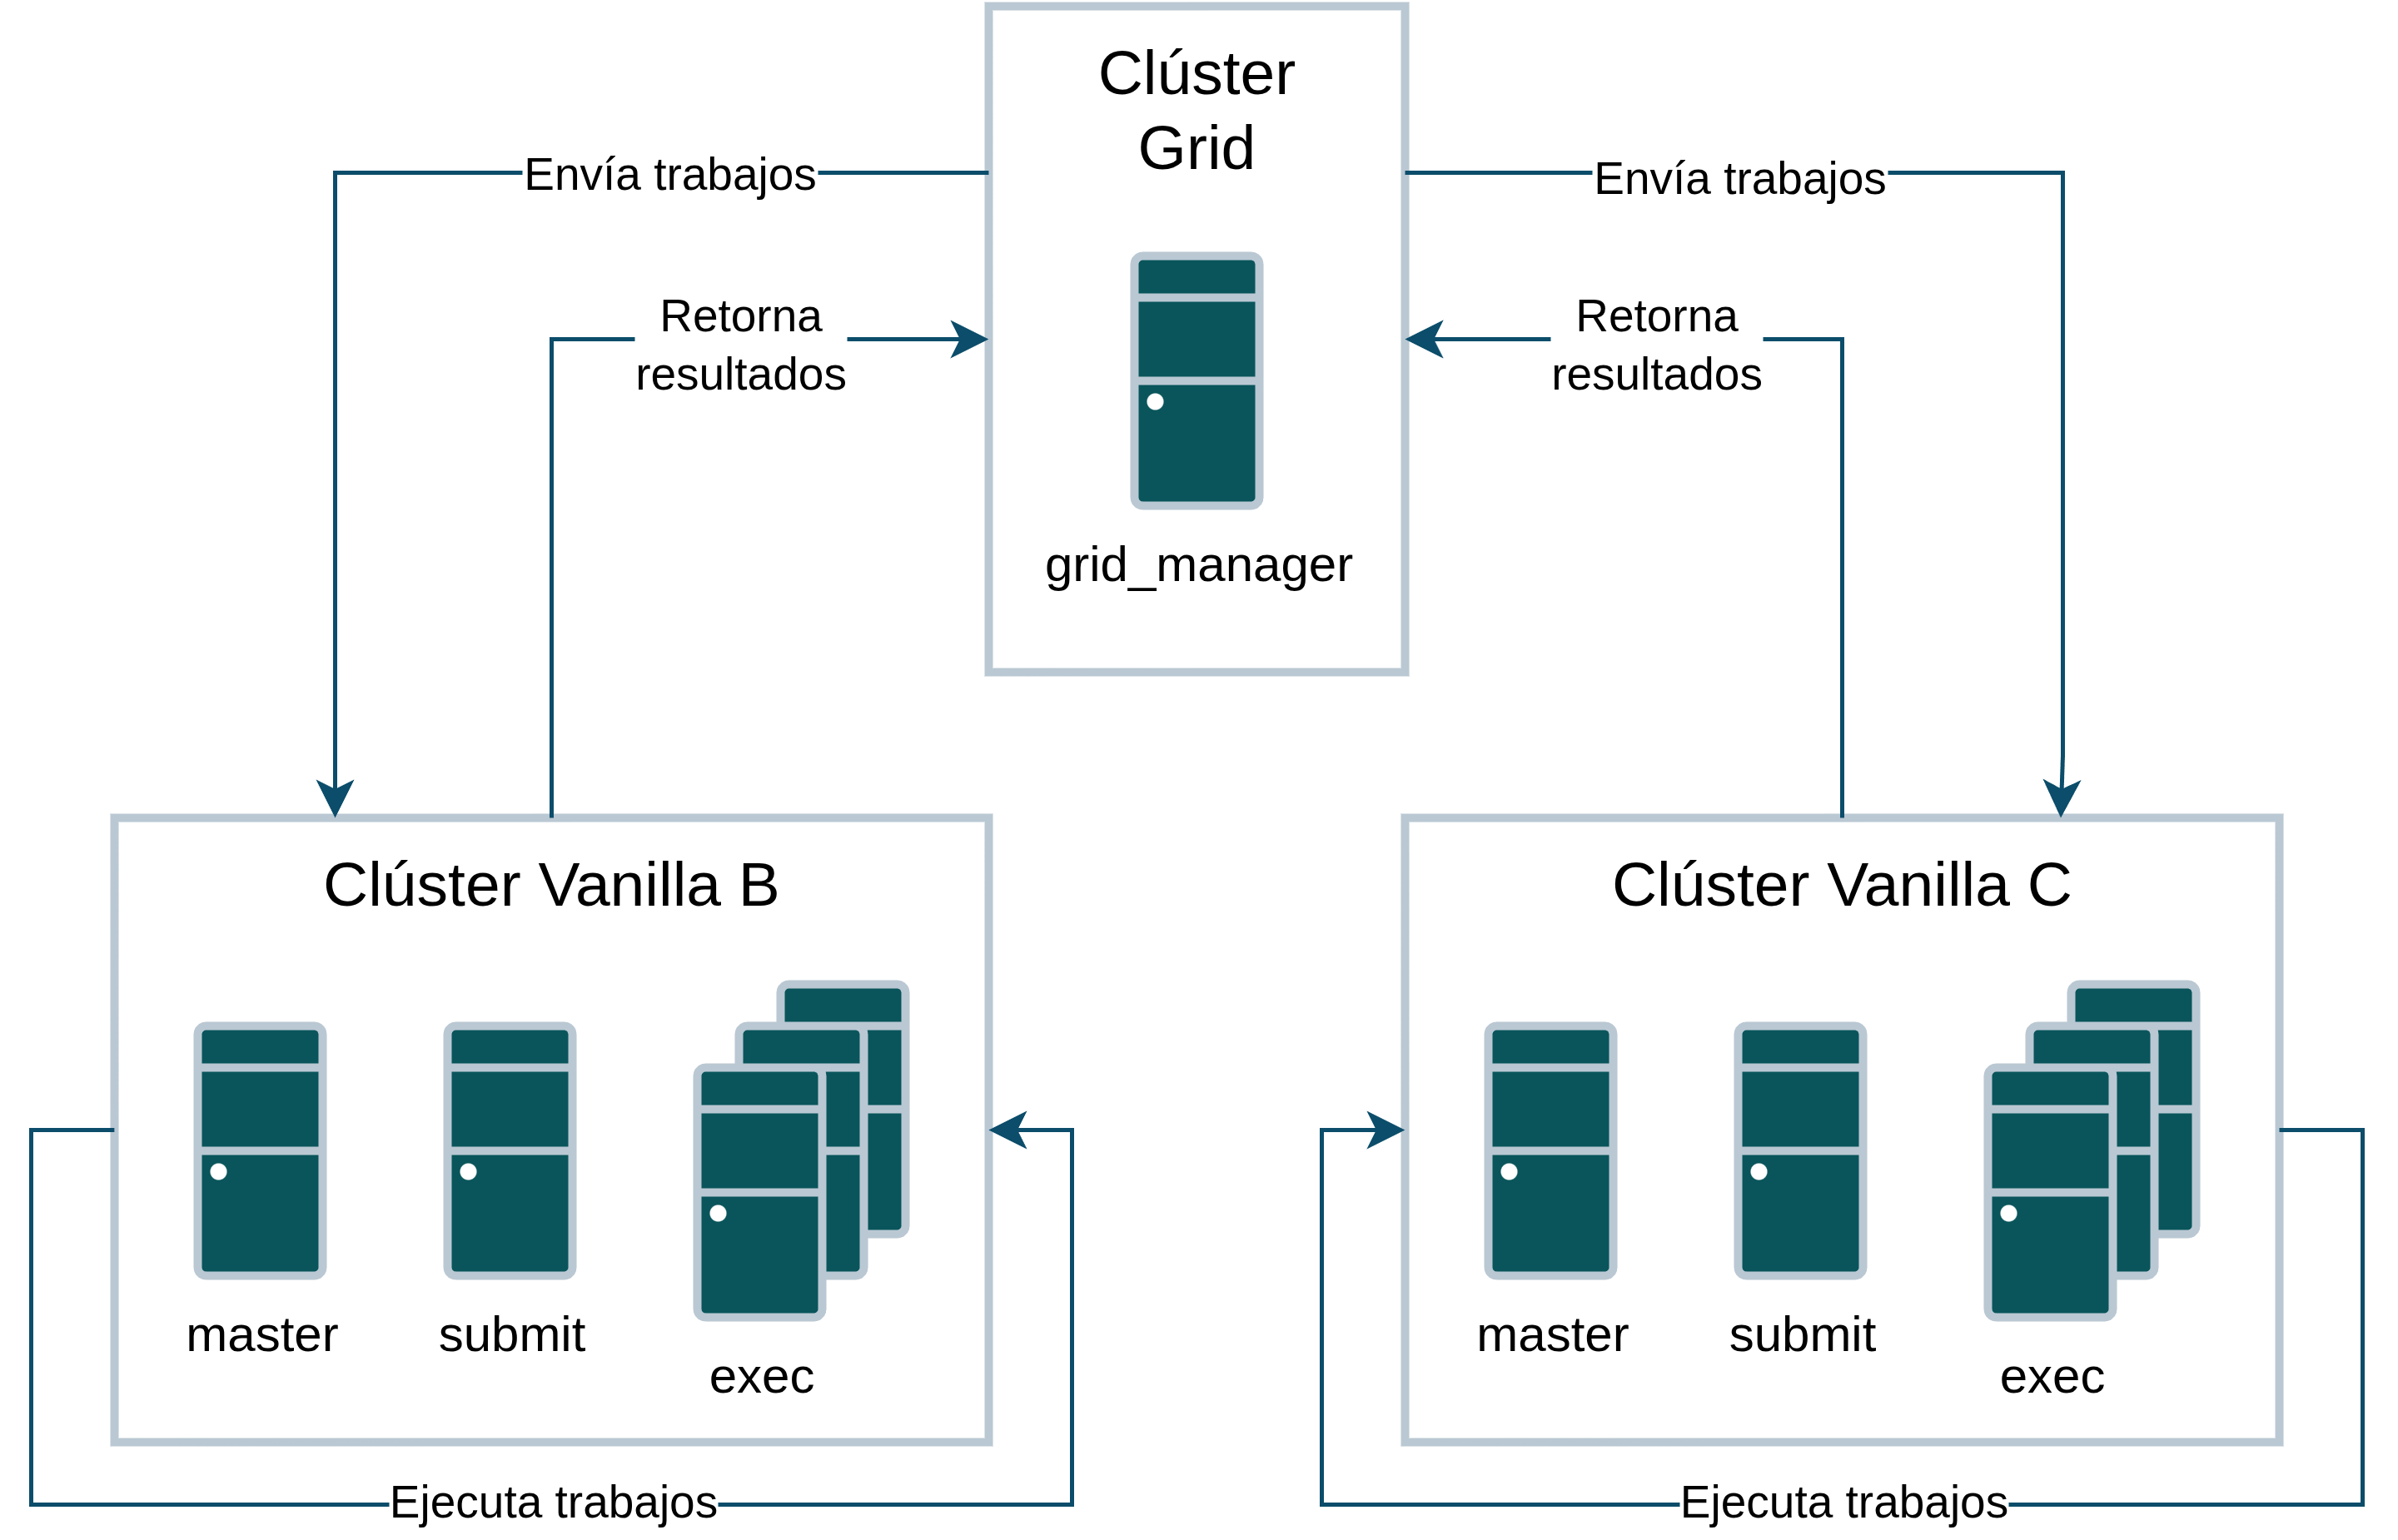
\includegraphics[scale=0.11]{apendices/infra-virtual/Diagramas HTCondor-Grid-flow.drawio.png}
	\caption{Arquitectura del universo Grid en la infraestructura HTCondor del~\GRID}
	\label{fig:grid-architecture}
\end{figure}

\FloatBarrier\subsubsection{Configuración del \textit{grid manager}}

El \textit{grid manager} constituye el componente central del universo Grid, implementando la lógica de distribución de trabajos y coordinación con clústeres remotos. Su configuración se basa en el archivo \texttt{/etc/condor/condor\_config.local} que define los parámetros específicos para su rol.

\textbf{Configuración de \textit{daemons}:}

La configuración especifica los \textit{daemons} que se ejecutan en el \textit{grid manager}:

\begin{minted}[
    frame=lines,
    framesep=2mm,
    baselinestretch=1.2,
    bgcolor=lightgray!10,
    fontsize=\footnotesize,
]{bash}
# Daemons ejecutados en el grid manager
DAEMON_LIST = SCHEDD, MASTER, GRIDMANAGER, COLLECTOR
\end{minted}

\textbf{Configuración específica del universo Grid:}

\begin{minted}[
    frame=lines,
    framesep=2mm,
    baselinestretch=1.2,
    bgcolor=lightgray!10,
    fontsize=\footnotesize,
]{bash}
# Variables específicas para el universo Grid
CONDOR_GAHP = $(SBIN)/condor_c-gahp
C_GAHP_LOG = /tmp/CGAHPLog.$(USERNAME)
C_GAHP_WORKER_THREAD_LOG = /tmp/CGAHPWorkerLog.$(USERNAME)
C_GAHP_WORKER_THREAD_LOCK = /tmp/CGAHPWorkerLock.$(USERNAME)
\end{minted}

\textbf{Configuración de seguridad:}

La configuración de seguridad implementa autenticación opcional para facilitar la comunicación entre nodos en una red confiable:

\begin{minted}[
    frame=lines,
    framesep=2mm,
    baselinestretch=1.2,
    bgcolor=lightgray!10,
    fontsize=\footnotesize,
]{bash}
# Configuración de seguridad minima para cluster en red confiable
SEC_DEFAULT_AUTHENTICATION = OPTIONAL
SEC_DEFAULT_AUTHENTICATION_METHODS = CLAIMTOBE,FS
SEC_DEFAULT_ENCRYPTION = OPTIONAL
SEC_DEFAULT_INTEGRITY = OPTIONAL
\end{minted}

\textbf{Permisos de acceso:}

\begin{minted}[
    frame=lines,
    framesep=2mm,
    baselinestretch=1.2,
    bgcolor=lightgray!10,
    fontsize=\footnotesize,
]{bash}
# Permisos para el daemon SCHEDD
ALLOW_READ_SCHEDD = 172.30.27.43, 127.0.0.1, rb3-*
ALLOW_WRITE_SCHEDD = 172.30.27.43, 127.0.0.1, rb3-*

# Permisos generales de red
ALLOW_READ  = 172.30.*
ALLOW_WRITE = 172.30.*
\end{minted}

\textbf{Configuración de red:}

\begin{minted}[
    frame=lines,
    framesep=2mm,
    baselinestretch=1.2,
    bgcolor=lightgray!10,
    fontsize=\footnotesize,
]{bash}
# Configuración de interfaz de red específica
BIND_ALL_INTERFACES = FALSE
NETWORK_INTERFACE = 172.30.27.11

# Configuración de dominio
FILESYSTEM_DOMAIN = $(FULL_HOSTNAME)
UID_DOMAIN = uniquindio.edu.co
CONDOR_HOST = rb3-t01-1
\end{minted}

\FloatBarrier\subsection{Configuración de clústeres Vanilla}

Los clústeres Vanilla constituyen los recursos computacionales donde se ejecutan finalmente los trabajos distribuidos desde el clúster Grid. La configuración de estos clústeres fue adaptada durante este proyecto para habilitar la recepción y ejecución de trabajos provenientes del universo Grid.

\FloatBarrier\subsubsection{Configuración del nodo \textit{submit}}

El nodo \textit{submit} de cada clúster Vanilla actúa como punto de entrada para trabajos provenientes del \textit{grid manager}. Su configuración habilita tanto funcionalidades locales como la capacidad de recibir trabajos remotos.

\textbf{Configuración de \textit{daemons}:}

\begin{minted}[
    frame=lines,
    framesep=2mm,
    baselinestretch=1.2,
    bgcolor=lightgray!10,
    fontsize=\footnotesize,
]{bash}
# Daemons ejecutados en el nodo submit
DAEMON_LIST = SCHEDD, MASTER
\end{minted}

\textbf{Habilitación del universo Grid:}

\begin{minted}[
    frame=lines,
    framesep=2mm,
    baselinestretch=1.2,
    bgcolor=lightgray!10,
    fontsize=\footnotesize,
]{bash}
# Habilitación explícita del universo Grid
ENABLE_GRID_UNIVERSE = True

# Configuración específica para SCHEDD
SCHEDD_ADDRESS_FILE = $(LOG)/.schedd_address
BIND_ALL_INTERFACES = FALSE
\end{minted}

\textbf{Permisos para grid manager:}

\begin{minted}[
    frame=lines,
    framesep=2mm,
    baselinestretch=1.2,
    bgcolor=lightgray!10,
    fontsize=\footnotesize,
]{bash}
# Permisos específicos para grid manager
ALLOW_WRITE_SCHEDD = 172.30.27.43, 127.0.0.1
ALLOW_READ_SCHEDD = 172.30.27.43, 127.0.0.1
HOSTALLOW_WRITE = 172.30.27.43, 127.0.0.1
\end{minted}

\textbf{Configuración de usuarios y autenticación:}

Una configuración crítica para el funcionamiento del universo Grid es la gestión de usuarios y autenticación entre nodos:

\begin{minted}[
    frame=lines,
    framesep=2mm,
    baselinestretch=1.2,
    bgcolor=lightgray!10,
    fontsize=\footnotesize,
]{bash}
# Usuarios con privilegios especiales
QUEUE_SUPER_USERS = root, condor, CONDOR_ANONYMOUS_USER, alma
UID_DOMAIN = gridmanager

# Habilitación de usuarios anónimos
ALLOW_WRITE = *, anonymous@*
ALLOW_READ = *, anonymous@*
ALLOW_ADMINISTRATOR = *, $(FULL_HOSTNAME), $(IP_ADDRESS)
ALLOW_OWNER = *

# Usuario anónimo para condor
CONDOR_ANONYMOUS_USER = nobody

# Configuración de autenticación
SEC_READ_AUTHENTICATION = OPTIONAL
SEC_WRITE_AUTHENTICATION = OPTIONAL
SEC_ADMINISTRATOR_AUTHENTICATION = OPTIONAL

SCHEDD.ALLOW_ANONYMOUS_USER = TRUE
\end{minted}

\FloatBarrier\subsubsection{Configuración del nodo \textit{master/central manager}}

El nodo \textit{master/central manager} de cada clúster Vanilla coordina los recursos locales y facilita la comunicación con el \textit{grid manager}:

\textbf{Configuración de \textit{daemons}:}

\begin{minted}[
    frame=lines,
    framesep=2mm,
    baselinestretch=1.2,
    bgcolor=lightgray!10,
    fontsize=\footnotesize,
]{bash}
# Daemons ejecutados en el central manager
DAEMON_LIST = COLLECTOR, NEGOTIATOR, MASTER
\end{minted}

\textbf{Configuración de red y permisos:}

\begin{minted}[
    frame=lines,
    framesep=2mm,
    baselinestretch=1.2,
    bgcolor=lightgray!10,
    fontsize=\footnotesize,
]{bash}
# Configuración de red específica para Clúster B
NETWORK_INTERFACE = 172.30.27.34  # Para central manager del Clúster B
# NETWORK_INTERFACE = 172.30.27.66  # Para central manager del Clúster C

# Nodo coordinador del clúster
CONDOR_HOST = rb3-t06-1  # Para Clúster B
# CONDOR_HOST = rb3-t06-4  # Para Clúster C

# Permisos de red amplios para comunicación Grid
ALLOW_READ  = 172.30.*
ALLOW_WRITE = 172.30.*
\end{minted}

\FloatBarrier\subsubsection{Configuración de nodos \textit{Execute}}

Los nodos \textit{Execute} proporcionan los recursos computacionales donde se ejecutan los trabajos. Su configuración permite recibir trabajos tanto locales como provenientes del \textit{grid manager}:

\textbf{Configuración de \textit{daemons}:}

\begin{minted}[
    frame=lines,
    framesep=2mm,
    baselinestretch=1.2,
    bgcolor=lightgray!10,
    fontsize=\footnotesize,
]{bash}
# Daemons ejecutados en nodos Execute
DAEMON_LIST = STARTD, MASTER
\end{minted}

\FloatBarrier\subsection{Configuración de red y resolución de nombres}

Una configuración crítica para el funcionamiento del universo Grid es la resolución de nombres entre todos los nodos participantes. El archivo \texttt{/etc/hosts} en cada nodo debe contener las entradas correspondientes a todos los nodos de la infraestructura.

\textbf{Configuración completa del archivo \texttt{/etc/hosts}:}

\begin{minted}[
    frame=lines,
    framesep=2mm,
    baselinestretch=1.2,
    bgcolor=lightgray!10,
    fontsize=\footnotesize,
]{bash}
127.0.0.1       localhost

# grid manager
172.30.27.11    rb3-t01-1

# Clúster B - Vanilla
# master
172.30.27.34    rb3-t06-1
# submit
172.30.27.35    rb3-t06-2
# Execute nodes
172.30.27.36    rb3-t02-1
172.30.27.37    rb3-t02-2
172.30.27.38    rb3-t02-3
172.30.27.39    rb3-t02-4
172.30.27.40    rb3-t02-5
172.30.27.41    rb3-t02-6
172.30.27.42    rb3-t02-7
172.30.27.43    rb3-t03-2
172.30.27.44    rb3-t03-3
172.30.27.45    rb3-t03-4
172.30.27.46    rb3-t03-5
172.30.27.47    rb3-t03-6
172.30.27.48    rb3-t03-7

# Clúster C - Vanilla
# master
172.30.27.66    rb3-t06-4
# submit
172.30.27.67    rb3-t06-5
# Execute nodes
172.30.27.68    rb3-t04-1
172.30.27.69    rb3-t04-2
172.30.27.70    rb3-t04-3
172.30.27.71    rb3-t04-4
172.30.27.72    rb3-t04-6
172.30.27.73    rb3-t04-7
172.30.27.74    rb3-t05-1
172.30.27.75    rb3-t05-2
172.30.27.76    rb3-t05-3
172.30.27.77    rb3-t05-4
172.30.27.78    rb3-t05-5
172.30.27.79    rb3-t05-6
172.30.27.80    rb3-t05-7
\end{minted}

\FloatBarrier\subsection{Expansión de la infraestructura Vanilla}

Durante el desarrollo de este proyecto se realizó la expansión de la infraestructura Vanilla existente, pasando de un único clúster a dos clústeres independientes (Clúster B y Clúster C). Esta expansión fue necesaria para demostrar la capacidad de distribución de trabajos del universo Grid y proporcionar redundancia en la infraestructura.

\textbf{Beneficios de la expansión:}

\begin{itemize}
	\item \textbf{Mayor capacidad computacional}: Duplicación de los recursos disponibles para ejecución de trabajos.
	
	\item \textbf{Redundancia}: Capacidad de continuar operaciones en caso de falla de un clúster completo.
	
	\item \textbf{Balanceo de carga}: Distribución automática de trabajos según disponibilidad de recursos.
	
	\item \textbf{Escalabilidad}: Demostración de que la arquitectura puede expandirse a múltiples clústeres adicionales.
\end{itemize}

\FloatBarrier\subsection{Verificación de la configuración}

Una vez completada la configuración, es posible verificar el correcto funcionamiento del universo Grid mediante varios comandos de diagnóstico:

\textbf{Verificación desde el universo Grid:}

\begin{minted}[
    frame=lines,
    framesep=2mm,
    baselinestretch=1.2,
    bgcolor=lightgray!10,
    fontsize=\footnotesize,
]{bash}
# Verificar conectividad con clústeres remotos
condor_status -pool rb3-t06-1

# Verificar configuración local del SCHEDD
condor_config_val -schedd DAEMON_LIST

# Verificar logs del grid manager
tail -f /var/log/condor/GridmanagerLog
\end{minted}

\textbf{Verificación desde clústeres Vanilla:}

\begin{minted}[
    frame=lines,
    framesep=2mm,
    baselinestretch=1.2,
    bgcolor=lightgray!10,
    fontsize=\footnotesize,
]{bash}
# Verificar disponibilidad de recursos
condor_status

# Verificar permisos de grid manager
condor_config_val ALLOW_WRITE_SCHEDD
\end{minted}

\FloatBarrier\subsection{Consideraciones importantes}

\textbf{Limitaciones del alcance:}

Es importante destacar que este proyecto se enfocó específicamente en la adaptación de la infraestructura Vanilla existente para soportar trabajos provenientes del universo Grid. La instalación inicial de HTCondor en los dispositivos Raspberry Pi fue realizada previamente y no formó parte del alcance de este trabajo.

\textbf{Configuración específica del entorno:}

Las configuraciones presentadas están diseñadas para el entorno específico del Grupo \GRID, incluyendo:

\begin{itemize}
	\item Arquitectura ARM de 32 bits (armv7l)
	\item Sistema operativo Raspbian GNU/Linux 9 (stretch)
	\item HTCondor versión 8.4.11
	\item Red interna confiable (172.30.27.0/24)
\end{itemize}

\textbf{Escalabilidad de la solución:}

La configuración implementada permite la adición de clústeres Vanilla adicionales mediante la replicación de la configuración base y la actualización de las tablas de enrutamiento de red. Esta característica facilita el crecimiento futuro de la infraestructura según las necesidades computacionales del grupo de investigación.

\textbf{Seguridad y confiabilidad:}

La configuración de seguridad mínima (autenticación opcional) está justificada por el entorno de red confiable y controlado donde opera la infraestructura. En entornos de producción o redes menos confiables, sería necesario implementar políticas de seguridad más estrictas, incluyendo autenticación obligatoria y cifrado de comunicaciones.

\newpage


\phantomsection

% Increment the chapter counter so \thechapter shows the correct number
% and make it referenceable with \ref
\refstepcounter{chapter}
\label{chap:plantilla-dar}


% Manually add this appendix to the Table of Contents
\addcontentsline{toc}{chapter}{Apéndice \thechapter: Plantilla análisis DAR}

% Add vertical space above the title (mimics standard chapter spacing)
\vspace{40pt}

% Display the actual chapter title (centered, large, bold)
{\centering \normalfont\huge\bfseries Apéndice~\thechapter: Plantilla análisis DAR~\par}

% Add spacing between title and horizontal rule
\vspace{10pt}

% Draw a horizontal line across the page for visual separation
{\centering \rule{\textwidth}{0.4pt} \par}

% Add vertical space between title section and content
\vspace{40pt}

% Set the running headers for left and right pages
\markboth{Apéndice \thechapter: Plantilla análisis DAR}{Apéndice \thechapter: Plantilla análisis DAR}



\begin{table}[H]
	\centering
	\renewcommand{\arraystretch}{1.2} % Espaciado reducido
	\fontsize{9pt}{10pt}\selectfont % Tamaño de fuente 8pt
	\caption{Plantilla análisis \DAR.}
	\label{tab:plantilla-analisis_dar}
	\begin{tabular}{|>{\centering\arraybackslash}p{1.8cm}|>{\centering\arraybackslash}p{1.8cm}|>{\centering\arraybackslash}p{2.5cm}|>{\centering\arraybackslash}p{2.2cm}|>{\centering\arraybackslash}p{0.7cm}|>{\centering\arraybackslash}p{1.4cm}|>{\centering\arraybackslash}p{1.5cm}|}
		\hline
		{\scriptsize\textbf{Criterio}}                         & {\tiny\textbf{PARALLEL}}                                                   & {\tiny\textbf{CHECKPOINTING}}                          & {\tiny\textbf{POPULARITY}} & {\tiny\textbf{DOC}} & {\tiny\textbf{ROLE DIV}} & {\tiny\textbf{}} \\
		\hline
		{\cellcolor[HTML]{E6E6E6}\scriptsize\textbf{Universo}} & \multicolumn{5}{c|}{\cellcolor[HTML]{E6E6E6}{\scriptsize\textbf{Puntaje}}} & \cellcolor[HTML]{E6E6E6}{\scriptsize\textbf{Promedio}}                                                                                                  \\
		\hline
		Vanilla                                                &                                                                            &                                                        &                            &                     &                          &                  \\
		\hline
		Grid                                                   &                                                                            &                                                        &                            &                     &                          &                  \\
		\hline
		Java                                                   &                                                                            &                                                        &                            &                     &                          &                  \\
		\hline
		Scheduler                                              &                                                                            &                                                        &                            &                     &                          &                  \\
		\hline
		Local                                                  &                                                                            &                                                        &                            &                     &                          &                  \\
		\hline
		Parallel                                               &                                                                            &                                                        &                            &                     &                          &                  \\
		\hline
		VM                                                     &                                                                            &                                                        &                            &                     &                          &                  \\
		\hline
		Container                                              &                                                                            &                                                        &                            &                     &                          &                  \\
		\hline
		Docker                                                 &                                                                            &                                                        &                            &                     &                          &                  \\
		\hline
	\end{tabular}
	\vspace{5pt}
\end{table}

\newpage


\FloatBarrier\section{ACOFI 2024}
% SECCION DE ACOFI

En esta sección se presenta la ponencia presentada en el congreso ACOFI 2025 como
resultado de la investigación desarrollada en este trabajo.

\shadowfig{tablas-images/difusion/acofi/1.png}{Ponencia ACOFI --- Página 1}
\shadowfig{tablas-images/difusion/acofi/2.png}{Ponencia ACOFI --- Página 2}
\shadowfig{tablas-images/difusion/acofi/3.png}{Ponencia ACOFI --- Página 3}
\shadowfig{tablas-images/difusion/acofi/4.png}{Ponencia ACOFI --- Página 4}
\shadowfig{tablas-images/difusion/acofi/5.png}{Ponencia ACOFI --- Página 5}
\shadowfig{tablas-images/difusion/acofi/6.png}{Ponencia ACOFI --- Página 6}
\shadowfig{tablas-images/difusion/acofi/7.png}{Ponencia ACOFI --- Página 7}
\shadowfig{tablas-images/difusion/acofi/8.png}{Ponencia ACOFI --- Página 8}
\shadowfig{tablas-images/difusion/acofi/9.png}{Ponencia ACOFI --- Página 9}
\shadowfig{tablas-images/difusion/acofi/10.png}{Ponencia ACOFI --- Página 10}


\FloatBarrier\section{Artículo de investigación para \textbf{\textit{Computación y Sistemas}} --- 2025}

A continuación se muestra el Articulo para la revista \href{https://www.cys.cic.ipn.mx/ojs/index.php/CyS}{Computación y Sistemas}


\shadowfig{tablas-images/difusion/computacion-y-sistemas/portada.png}{Portada del articulo para revista \textit{Computación y Sistemas}

\shadowfig{tablas-images/difusion/computacion-y-sistemas/1.png}{Articulo para revista \textit{Computación y Sistemas} --- Página 1}
\shadowfig{tablas-images/difusion/computacion-y-sistemas/2.png}{Articulo para revista \textit{Computación y Sistemas} --- Página 2}
\shadowfig{tablas-images/difusion/computacion-y-sistemas/3.png}{Articulo para revista \textit{Computación y Sistemas} --- Página 3}
\shadowfig{tablas-images/difusion/computacion-y-sistemas/4.png}{Articulo para revista \textit{Computación y Sistemas} --- Página 4}
\shadowfig{tablas-images/difusion/computacion-y-sistemas/5.png}{Articulo para revista \textit{Computación y Sistemas} --- Página 5}
\shadowfig{tablas-images/difusion/computacion-y-sistemas/6.png}{Articulo para revista \textit{Computación y Sistemas} --- Página 6}
\shadowfig{tablas-images/difusion/computacion-y-sistemas/7.png}{Articulo para revista \textit{Computación y Sistemas} --- Página 7}
\shadowfig{tablas-images/difusion/computacion-y-sistemas/8.png}{Articulo para revista \textit{Computación y Sistemas} --- Página 8}
\shadowfig{tablas-images/difusion/computacion-y-sistemas/9.png}{Articulo para revista \textit{Computación y Sistemas} --- Página 9}
\shadowfig{tablas-images/difusion/computacion-y-sistemas/10.png}{Articulo para revista \textit{Computación y Sistemas} --- Página 10}
\shadowfig{tablas-images/difusion/computacion-y-sistemas/11.png}{Articulo para revista \textit{Computación y Sistemas} --- Página 11}
\shadowfig{tablas-images/difusion/computacion-y-sistemas/12.png}{Articulo para revista \textit{Computación y Sistemas} --- Página 12}
\shadowfig{tablas-images/difusion/computacion-y-sistemas/13.png}{Articulo para revista \textit{Computación y Sistemas} --- Página 13}
\shadowfig{tablas-images/difusion/computacion-y-sistemas/14.png}{Articulo para revista \textit{Computación y Sistemas} --- Página 14}
\shadowfig{tablas-images/difusion/computacion-y-sistemas/15.png}{Articulo para revista \textit{Computación y Sistemas} --- Página 15}
\shadowfig{tablas-images/difusion/computacion-y-sistemas/16.png}{Articulo para revista \textit{Computación y Sistemas} --- Página 16}
\shadowfig{tablas-images/difusion/computacion-y-sistemas/17.png}{Articulo para revista \textit{Computación y Sistemas} --- Página 17}
\shadowfig{tablas-images/difusion/computacion-y-sistemas/18.png}{Articulo para revista \textit{Computación y Sistemas} --- Página 18}
\shadowfig{tablas-images/difusion/computacion-y-sistemas/19.png}{Articulo para revista \textit{Computación y Sistemas} --- Página 19}
\shadowfig{tablas-images/difusion/computacion-y-sistemas/20.png}{Articulo para revista \textit{Computación y Sistemas} --- Página 20}
\shadowfig{tablas-images/difusion/computacion-y-sistemas/21.png}{Articulo para revista \textit{Computación y Sistemas} --- Página 21}
\shadowfig{tablas-images/difusion/computacion-y-sistemas/22.png}{Articulo para revista \textit{Computación y Sistemas} --- Página 22}
\shadowfig{tablas-images/difusion/computacion-y-sistemas/23.png}{Articulo para revista \textit{Computación y Sistemas} --- Página 23}
\shadowfig{tablas-images/difusion/computacion-y-sistemas/24.png}{Articulo para revista \textit{Computación y Sistemas} --- Página 24}
\shadowfig{tablas-images/difusion/computacion-y-sistemas/25.png}{Articulo para revista \textit{Computación y Sistemas} --- Página 25}
\shadowfig{tablas-images/difusion/computacion-y-sistemas/26.png}{Articulo para revista \textit{Computación y Sistemas} --- Página 26}
\shadowfig{tablas-images/difusion/computacion-y-sistemas/27.png}{Articulo para revista \textit{Computación y Sistemas} --- Página 27}
\shadowfig{tablas-images/difusion/computacion-y-sistemas/28.png}{Articulo para revista \textit{Computación y Sistemas} --- Página 28}
\shadowfig{tablas-images/difusion/computacion-y-sistemas/29.png}{Articulo para revista \textit{Computación y Sistemas} --- Página 29}
\shadowfig{tablas-images/difusion/computacion-y-sistemas/30.png}{Articulo para revista \textit{Computación y Sistemas} --- Página 30}


% !TODO, aquí va el segúndo articulo
%\FloatBarrier\section{EDUTEC 2024}
%\input{apendices/difusion/edutec.tex}
%
\FloatBarrier\section{CEIFI 2025}
A continuación se muestran las diapositivas elaboradas para las ponencias del CEIFI 2025-02.

\shadowfig{tablas-images/difusion/CEIFI-2025-02/1.png}{Ponencia para CEIFI 2025-02 ---  Diapositiva 1}
\shadowfig{tablas-images/difusion/CEIFI-2025-02/2.png}{Ponencia para CEIFI 2025-02 ---  Diapositiva 2}
\shadowfig{tablas-images/difusion/CEIFI-2025-02/3.png}{Ponencia para CEIFI 2025-02 ---  Diapositiva 3}
\shadowfig{tablas-images/difusion/CEIFI-2025-02/4.png}{Ponencia para CEIFI 2025-02 ---  Diapositiva 4}
\shadowfig{tablas-images/difusion/CEIFI-2025-02/5.png}{Ponencia para CEIFI 2025-02 ---  Diapositiva 5}
\shadowfig{tablas-images/difusion/CEIFI-2025-02/6.png}{Ponencia para CEIFI 2025-02 ---  Diapositiva 6}
\shadowfig{tablas-images/difusion/CEIFI-2025-02/7.png}{Ponencia para CEIFI 2025-02 ---  Diapositiva 7}
\shadowfig{tablas-images/difusion/CEIFI-2025-02/8.png}{Ponencia para CEIFI 2025-02 ---  Diapositiva 8}
\shadowfig{tablas-images/difusion/CEIFI-2025-02/9.png}{Ponencia para CEIFI 2025-02 ---  Diapositiva 9}
\shadowfig{tablas-images/difusion/CEIFI-2025-02/10.png}{Ponencia para CEIFI 2025-02 ---  Diapositiva 10}
\shadowfig{tablas-images/difusion/CEIFI-2025-02/11.png}{Ponencia para CEIFI 2025-02 ---  Diapositiva 11}
\shadowfig{tablas-images/difusion/CEIFI-2025-02/12.png}{Ponencia para CEIFI 2025-02 ---  Diapositiva 12}
\shadowfig{tablas-images/difusion/CEIFI-2025-02/13.png}{Ponencia para CEIFI 2025-02 ---  Diapositiva 13}
\shadowfig{tablas-images/difusion/CEIFI-2025-02/14.png}{Ponencia para CEIFI 2025-02 ---  Diapositiva 14}
\shadowfig{tablas-images/difusion/CEIFI-2025-02/15.png}{Ponencia para CEIFI 2025-02 ---  Diapositiva 15}
\shadowfig{tablas-images/difusion/CEIFI-2025-02/16.png}{Ponencia para CEIFI 2025-02 ---  Diapositiva 16}
\shadowfig{tablas-images/difusion/CEIFI-2025-02/17.png}{Ponencia para CEIFI 2025-02 ---  Diapositiva 17}
\shadowfig{tablas-images/difusion/CEIFI-2025-02/18.png}{Ponencia para CEIFI 2025-02 ---  Diapositiva 18}
\shadowfig{tablas-images/difusion/CEIFI-2025-02/19.png}{Ponencia para CEIFI 2025-02 ---  Diapositiva 19}
\shadowfig{tablas-images/difusion/CEIFI-2025-02/20.png}{Ponencia para CEIFI 2025-02 ---  Diapositiva 20}
\shadowfig{tablas-images/difusion/CEIFI-2025-02/21.png}{Ponencia para CEIFI 2025-02 ---  Diapositiva 21}
\shadowfig{tablas-images/difusion/CEIFI-2025-02/22.png}{Ponencia para CEIFI 2025-02 ---  Diapositiva 22}
\shadowfig{tablas-images/difusion/CEIFI-2025-02/23.png}{Ponencia para CEIFI 2025-02 ---  Diapositiva 23}
\shadowfig{tablas-images/difusion/CEIFI-2025-02/24.png}{Ponencia para CEIFI 2025-02 ---  Diapositiva 24}
\shadowfig{tablas-images/difusion/CEIFI-2025-02/25.png}{Ponencia para CEIFI 2025-02 ---  Diapositiva 25}
\shadowfig{tablas-images/difusion/CEIFI-2025-02/26.png}{Ponencia para CEIFI 2025-02 ---  Diapositiva 26}
\shadowfig{tablas-images/difusion/CEIFI-2025-02/27.png}{Ponencia para CEIFI 2025-02 ---  Diapositiva 27}
\shadowfig{tablas-images/difusion/CEIFI-2025-02/28.png}{Ponencia para CEIFI 2025-02 ---  Diapositiva 28}

%
\FloatBarrier\section{GRID 2025-I }
A continuación la ponencia del grupo GRID presentada en el primer semestre del año 2025

%
\FloatBarrier\section{Póster GRID 2024-II}

\shadowfig{tablas-images/difusion/GRID-2024-02/poster.png}{Póster para ponencia de GRID 2024-02}









\end{document}
